%% GENERATED by scripts/paper/build_paper.py from docs/analysis/register/findings.yaml -- do not edit by hand;
%% rewrite the prose in main.tex or change the register / scripts/paper/paper_text.json and rebuild.

\subsection{Each operator has a personal style --- individual, not a type}\label{sec:res:personal-style}

\regtext{\textbf{Summary.} Operators differ a great deal in how they use the assistants, and the differences are personal. We describe each session by ten habits (how often a strategy card is taken, how often Suggest is pressed, how long a decision takes, and so on). From those habits alone, a person's second session resembles their own first (median profile r = .48) and essentially nobody else's (r = $-$.01): their own session is in the closest three of 33 four times as often as chance (41\% vs 9\%), although the second session is a different scenario, and who the operator is explains about six times more of card-taking than the mission does. Six of the ten habits carry over clearly; one (topping up drones on single-type missions) does not at all. Between people, use of the two assistants is only loosely linked ($\rho$ $\approx$ .35), so leaning on one is not a fixed part of one overall ``delegate'' strategy (though within a person the two do rise and fall together from session to session). The styles do not fall into types, and nothing measured beforehand (attitude to AI, views on human authority, experience) predicts them. Strong evidence for a stable personal style; good evidence against types; ``no evidence'' (not ``evidence of no effect'') for disposition.} \par\noindent{\small\textit{Strength of evidence (register rating): strong. Your verdict: core.}}

\subsubsection{The habits we grade them on}\label{sec:res:personal-style:habits}

\noindent \passtag{numbers only}

\noindent \regtext{To compare styles we describe every 8-minute session by ten habits, each something the logs record at every decision. Seven concern the strategic tier (the strategy cards): how often a card is taken as offered; how often cards are previewed before choosing; how long a decision takes; whether, when building by hand, the operator does it before the cards have even appeared; whether a card is edited before committing; and how many drones are committed compared with the cautious Conservative card, on single-type and on multi-type missions. Three concern the tactical tier (Suggest): how often Suggest is pressed on a plan, whether a suggested plan is deployed unchanged, and whether Suggest is pressed when recovering from a failure. The chart shows each habit's spread over all 66 sessions in its own units. Most habits vary enormously between sessions (card uptake runs from 0\% to 100\% of a session's decisions); two are nearly universal (most sessions keep every suggested plan unchanged, and most never edit a card). The right-hand column previews the next results: how strongly each habit carries over from a person's first session to their second.} (Figure~\ref{fig:res:personal-style:habits})

\begin{figure}[H]
\centering
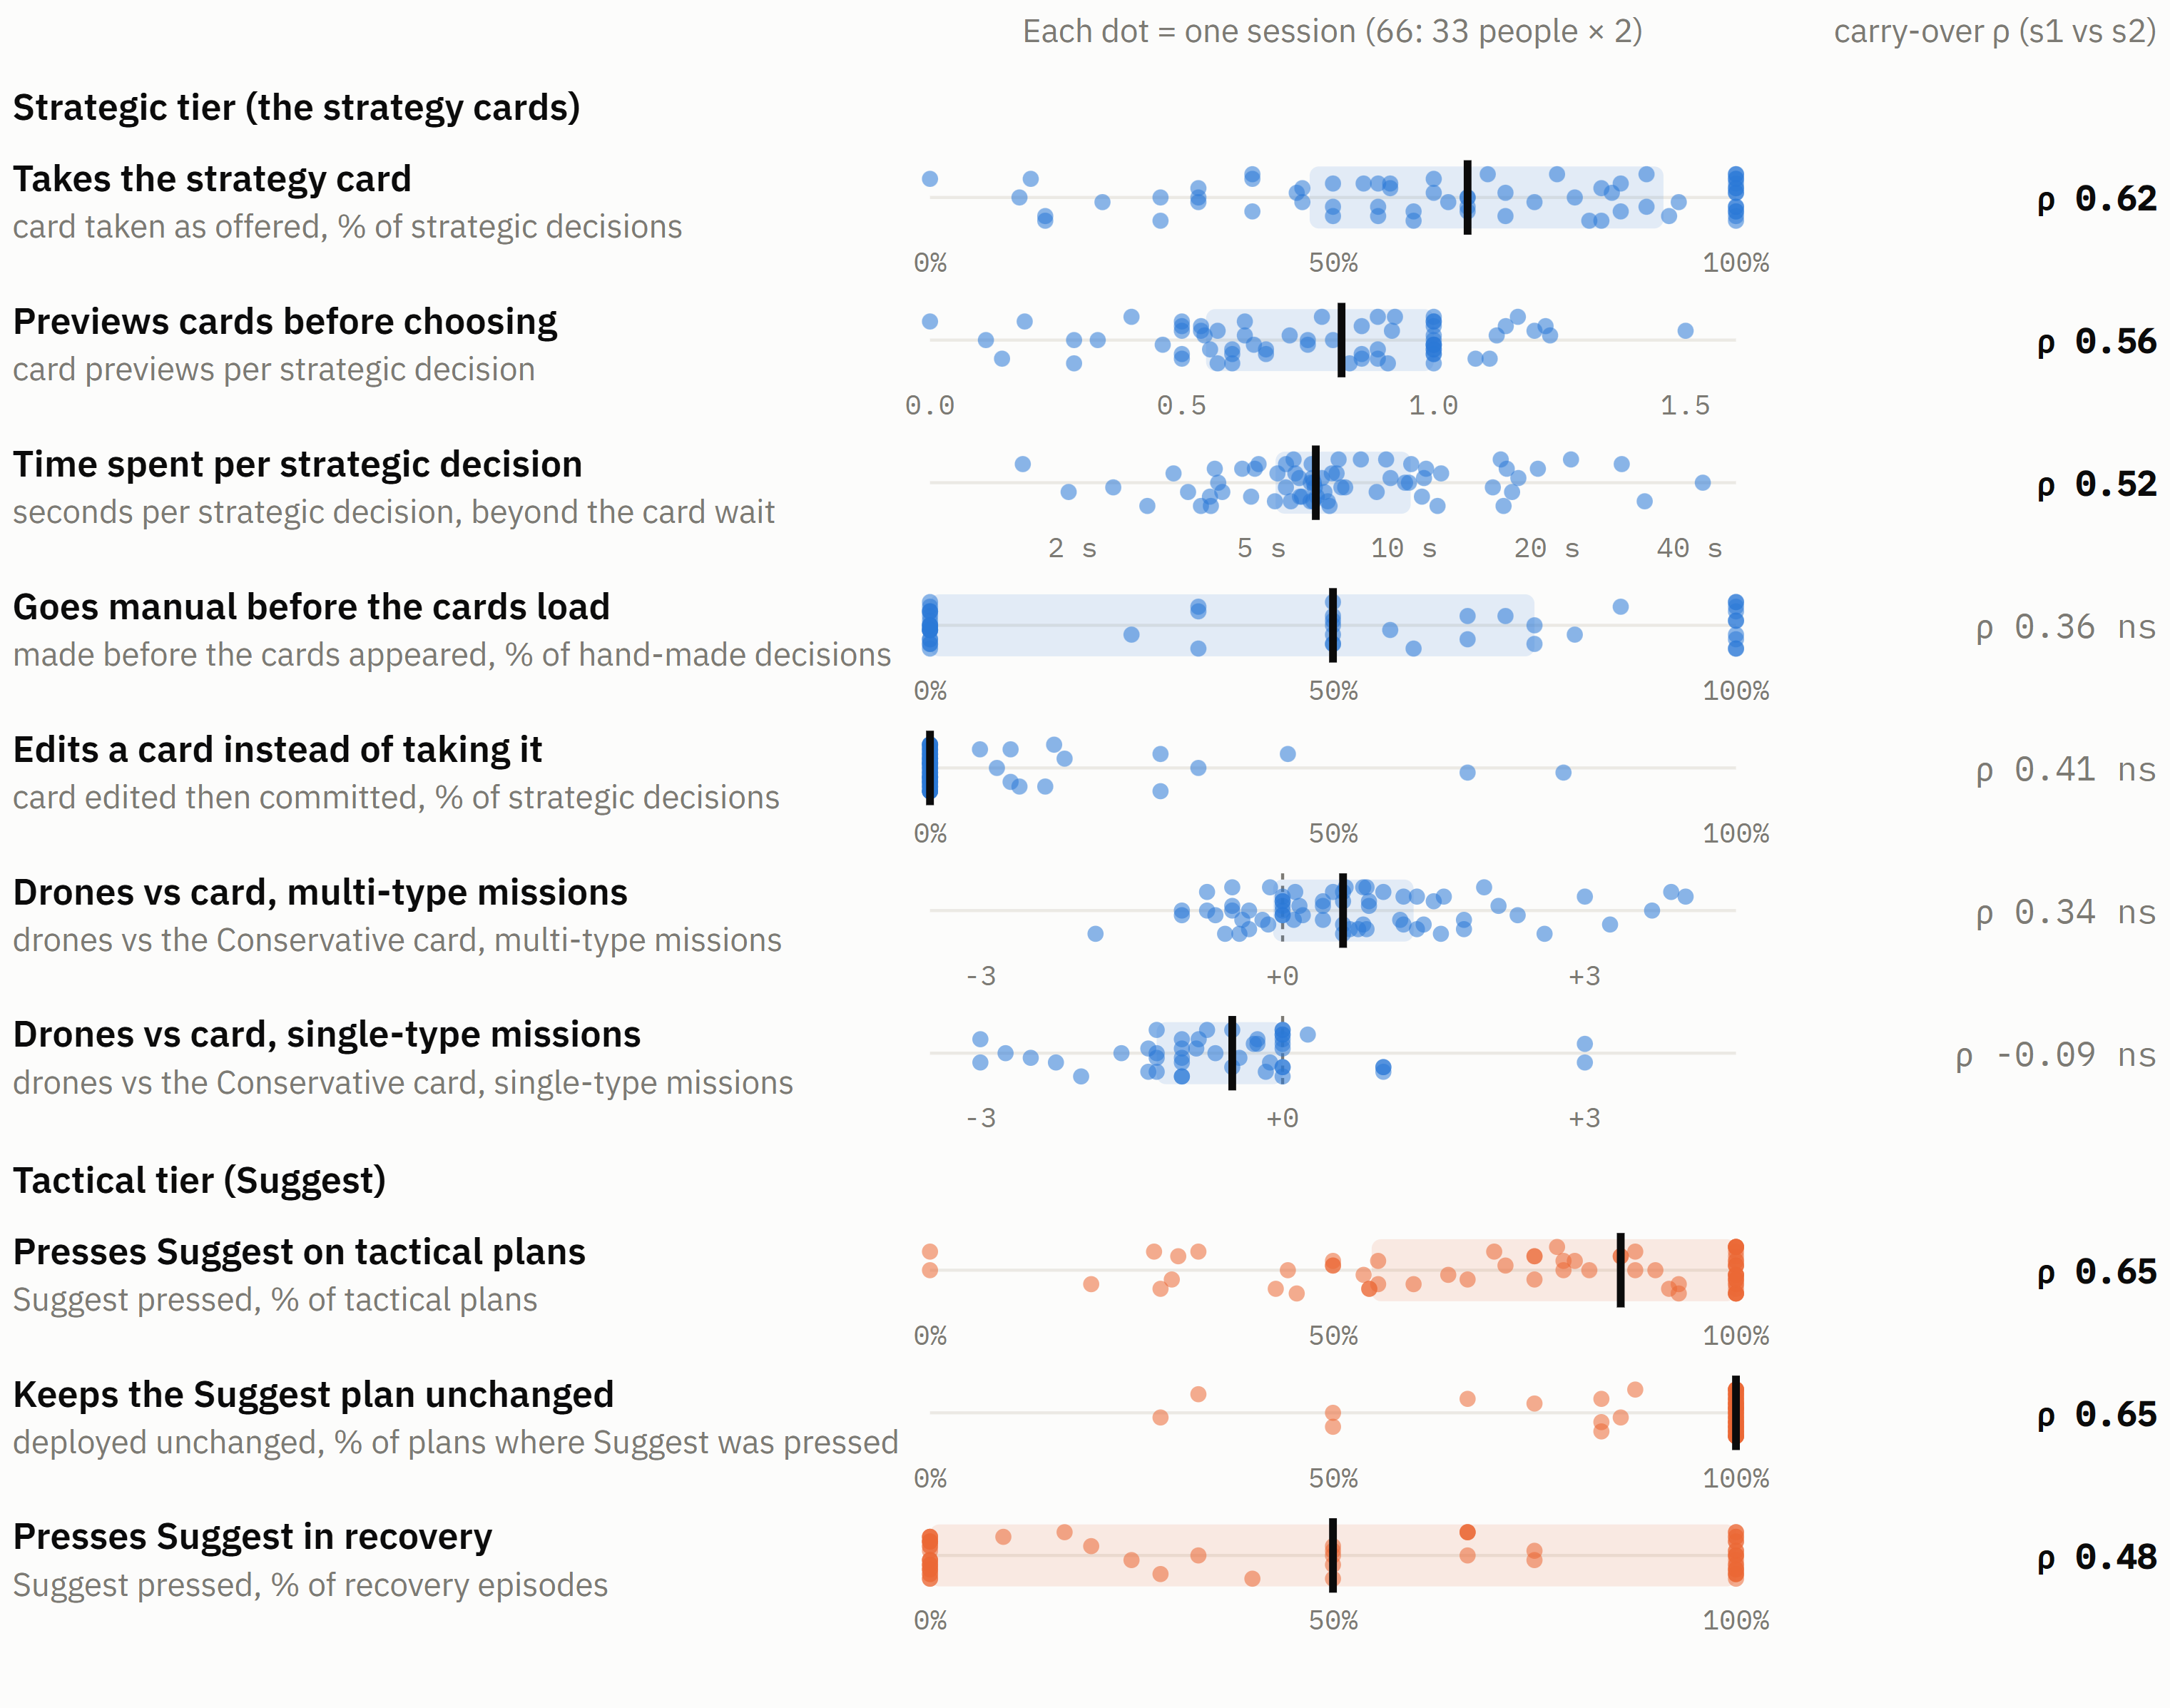
\includegraphics[width=\linewidth,height=0.55\textheight,keepaspectratio]{figs/results/f-personal-style__habits__main.png}
\caption{\textbf{The habits we grade them on}}
\label{fig:res:personal-style:habits}
\end{figure}

\paragraph*{Key numbers.}

\begin{itemize}[leftmargin=1.2em,itemsep=1pt]

\item Card taken as offered: median 67\% of a session's strategic decisions (middle half 47--91\%, range 0--100\%)

\item Suggest pressed: median 86\% of tactical plans (55--100\%); suggested plan kept unchanged: median 100\% (middle half 100--100\%)

\item Decision time beyond the card wait: median 6.5 s (5.4--10.3 s, range 1.6--43 s)

\item Card edited before committing: median 0\% (most sessions never); going manual before the cards appear: median 50\% of hand-made decisions (0--75\%)

\item Drones vs the Conservative card: single-type $-$0.5 ($-$1.25 to 0); multi-type +0.6 ($-$0.1 to +1.3)

\end{itemize}

\paragraph*{Method.} {\small Rows: 66 sessions (33 people $\times$ 2; P09 excluded). Each habit is a share or an average over that session's decisions. A habit with nothing to count in a session is undefined there: going manual before the cards (no hand-made decisions) in 15 sessions, drones on single-type missions (no single-type mission opened) in 19, Suggest in recovery (no failures) in 4, keeping the Suggest plan (Suggest never pressed) in 2. For the profiles these are filled with the median of that game. Decision time is analysed as log(1 + seconds) and shown in seconds. For the comparisons that follow, each habit is turned into a z-score among the sessions of the same game (each of the four fixed games), so a profile says how a person compares with others who faced the same missions. The ten habits were fixed in round 1 (H1) before any grouping was tried; outcomes (score, trust, questionnaires) are never among them. $\rho$ = Spearman correlation between a person's session-1 and session-2 values, game-adjusted (see ``How far each habit holds'').}

\paragraph*{What participants said.} \regtext{Asked to describe their approach, 15 of 33 named a consistent strategy of their own (C01). In their own words it is mostly about the habits graded here: whether they wait for the cards or go manual before they load (P21, P32), whether they trim or edit a card, whether they start from Suggest and touch it up (P31, P21), and how they check (P14, P17). Few described a rule for when to press Suggest. Most said they pressed it on nearly everything.}

\clearpage

\subsubsection{Where each person's own session ranks}\label{sec:res:personal-style:fingerprint-ranks}

\noindent \passtag{for the paper}

\noindent \regtext{Each person's ten-habit profile from session 1 is compared with all 33 session-2 profiles, and the 33 are ranked from most to least alike (and the same the other way round, session 2 among the session 1s). If habits were not personal, a person's own other session would be equally likely to land anywhere in that ranking (dashed line). Instead it is the single closest match 12 times out of 66 (2 expected by chance) and in the closest three 27 times (6 expected), even though the second session is a different scenario.} (Figure~\ref{fig:res:personal-style:fingerprint-ranks})

\begin{figure}[H]
\centering
\begin{subfigure}[t]{\linewidth}
\centering
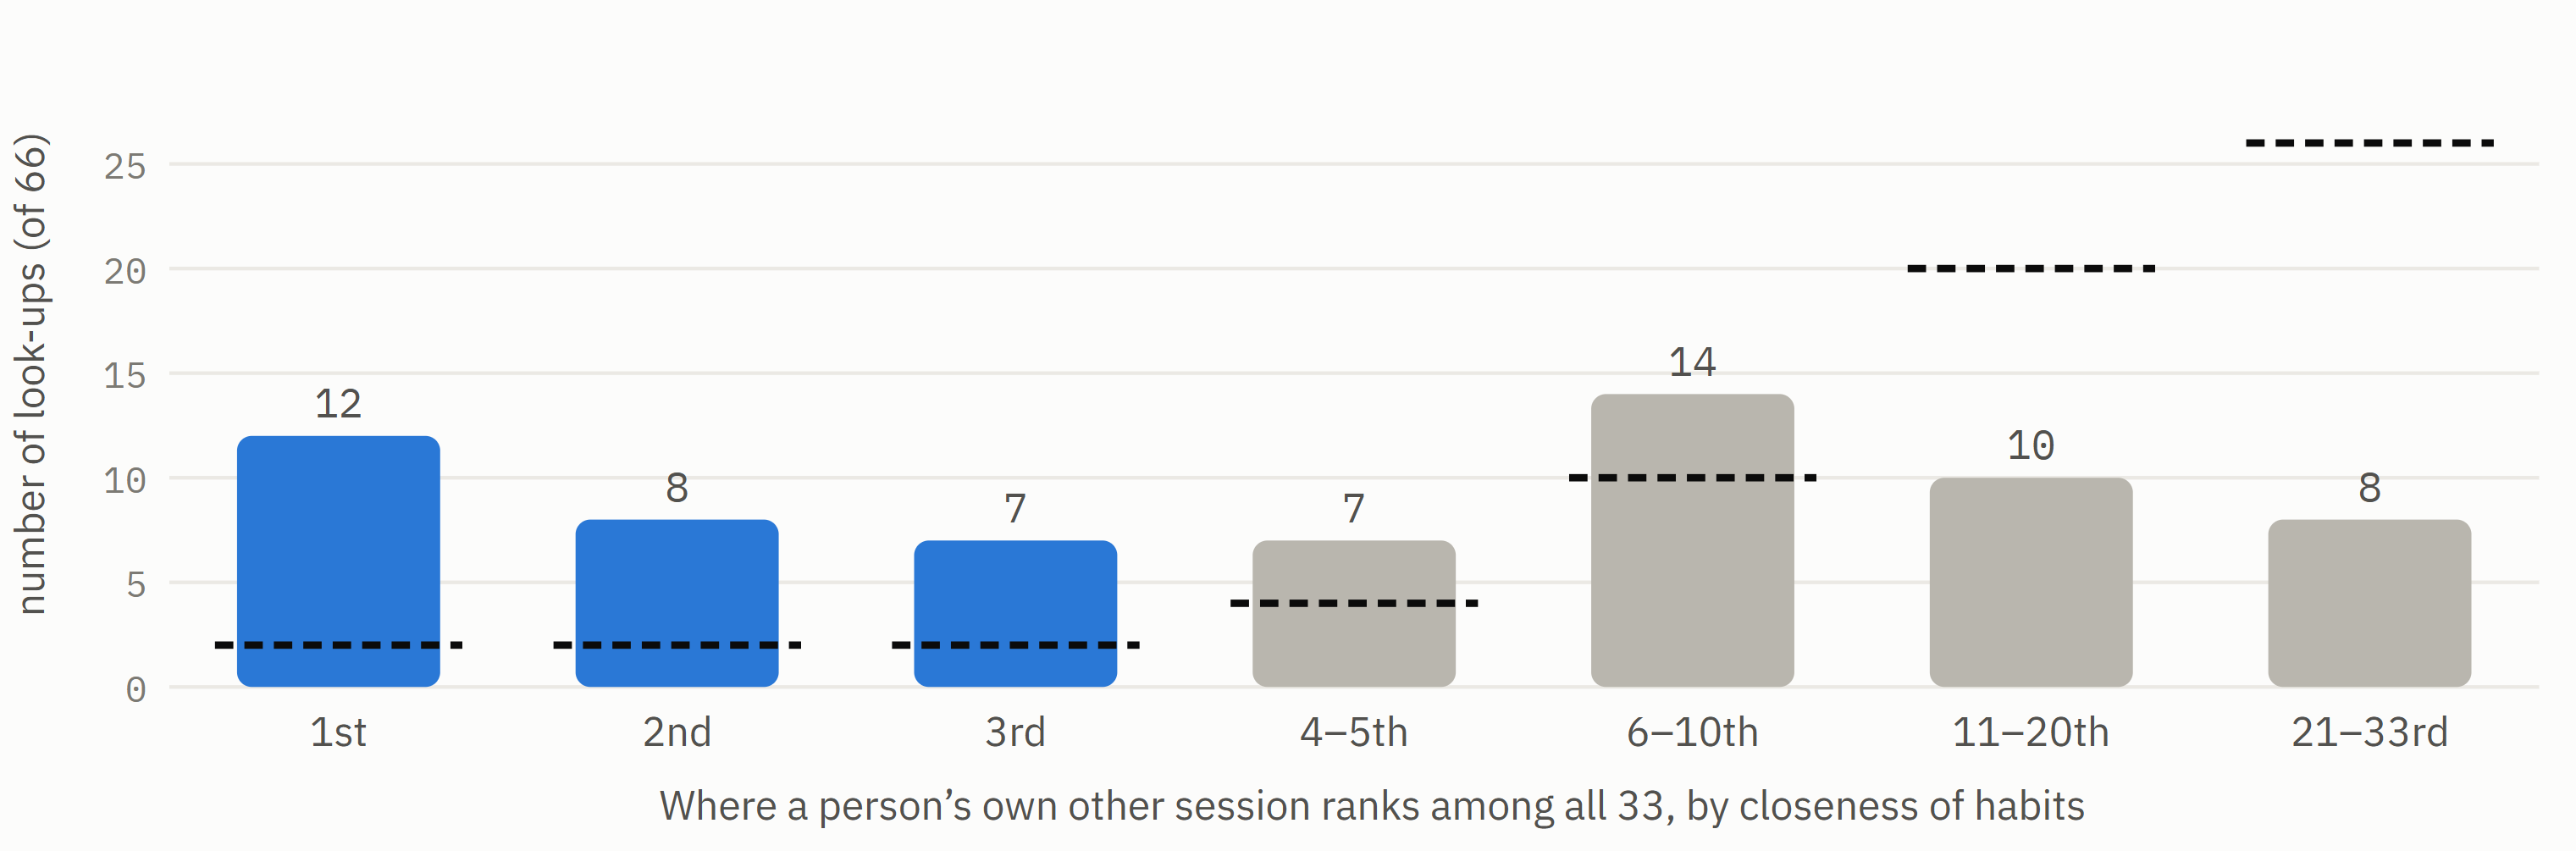
\includegraphics[width=\linewidth,height=0.23\textheight,keepaspectratio]{figs/results/f-personal-style__fingerprint-ranks__all.png}
\caption{All ten habits.}
\label{fig:res:personal-style:fingerprint-ranks:all}
\end{subfigure}
\par\smallskip
\begin{subfigure}[t]{\linewidth}
\centering
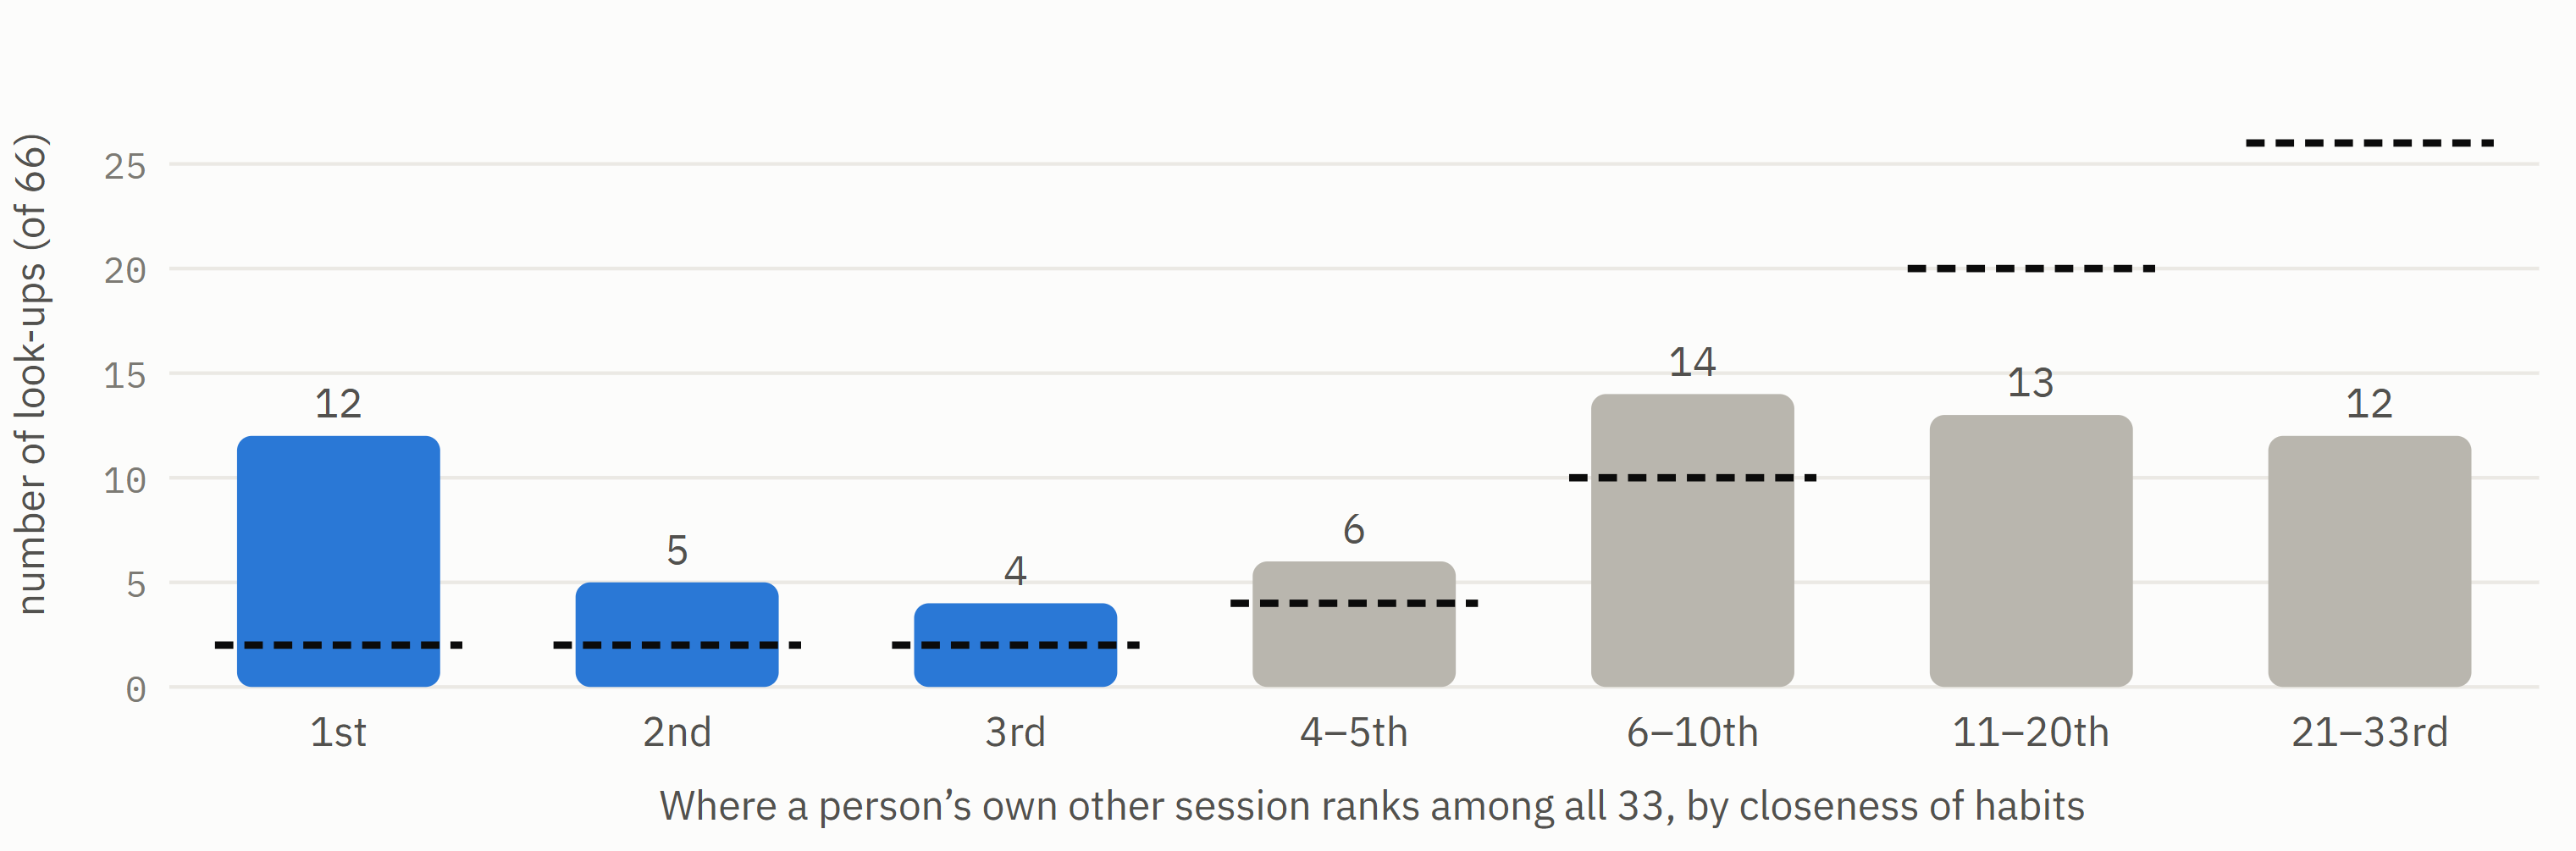
\includegraphics[width=\linewidth,height=0.23\textheight,keepaspectratio]{figs/results/f-personal-style__fingerprint-ranks__noaxis.png}
\caption{With the reliance axis removed.}
\label{fig:res:personal-style:fingerprint-ranks:noaxis}
\end{subfigure}
\par\smallskip
\caption{\textbf{Where each person's own session ranks}}
\label{fig:res:personal-style:fingerprint-ranks}
\end{figure}

\paragraph*{Key numbers.}

\begin{itemize}[leftmargin=1.2em,itemsep=1pt]

\item Own session ranked 1st: 12 of 66 look-ups vs 2 expected; in the closest three: 27 vs 6 (41\% vs 9\%); permutation p < .001

\item Average rank of own session 8.2 of 33 (chance 17.0); with the reliance axis removed 10.1 (p < .001)

\item Profile correlation with own other session: median r = .48; with other people's: median r = $-$.01; own closer for 29 of 33

\end{itemize}

\paragraph*{Method.} {\small Rows: 66 sessions (33 people $\times$ 2). Each session is the ten habits of the first section, each turned into a z-score among the sessions of the same game, so a profile says how this person compares with others who played that game. ``Alike'' = straight-line (Euclidean) distance between two ten-habit profiles. 66 look-ups (33 people, both directions); under chance every rank 1--33 is equally likely, so the dashed line is 66 $\times$ (ranks in the bin) / 33. The p-value shuffles who-is-who among the session-2 profiles 10 000 times. ``Reliance axis removed'' subtracts each profile's score on the first principal component (see the axis numbers) before comparing.}

\paragraph*{What participants said.} \regtext{Nobody was asked to compare their two sessions directly. In the think-aloud, though, several people open session 2 with the same move and say the same thing as in session 1: P29 'start conservative' and does single-colour missions by hand, P11 builds all-blue missions themself, P21 hand-builds in parallel. That fits a recognisable personal style. The people who said they changed are in the retest section.}

\clearpage

\subsubsection{Who decides matters more than what is being decided}\label{sec:res:personal-style:who-vs-what}

\noindent \passtag{for the paper}

\noindent \regtext{Card uptake runs from 8\% to 100\% across people (median 61\%). Knowing \emph{who} is deciding predicts whether a card is taken about six times better than knowing everything about the mission and when it arrived. In plain terms: shown two decisions, one where a card was taken and one where it was not, and told only who made each, you would pick the right one 75\% of the time (a coin: 50\%; knowing only the mission: 63\%). A person's session-1 rate on its own still does it 71\% of the time for their session-2 decisions.} (Figure~\ref{fig:res:personal-style:who-vs-what})

\begin{figure}[H]
\centering
\begin{subfigure}[t]{\linewidth}
\centering
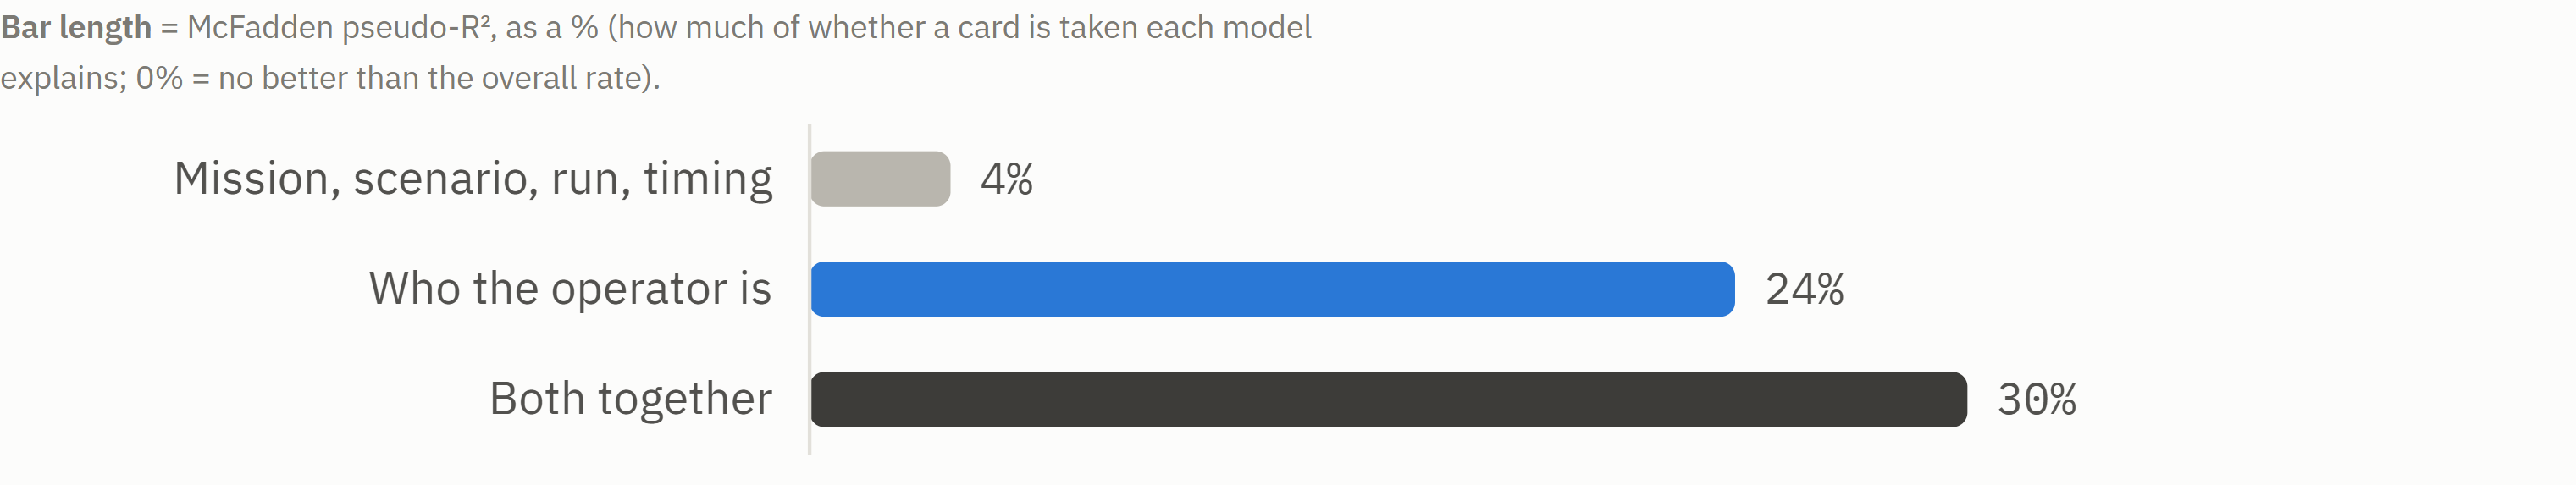
\includegraphics[width=\linewidth,height=0.23\textheight,keepaspectratio]{figs/results/f-personal-style__who-vs-what__r2.png}
\caption{McFadden pseudo-$R^2$.}
\label{fig:res:personal-style:who-vs-what:r2}
\end{subfigure}
\par\smallskip
\begin{subfigure}[t]{\linewidth}
\centering
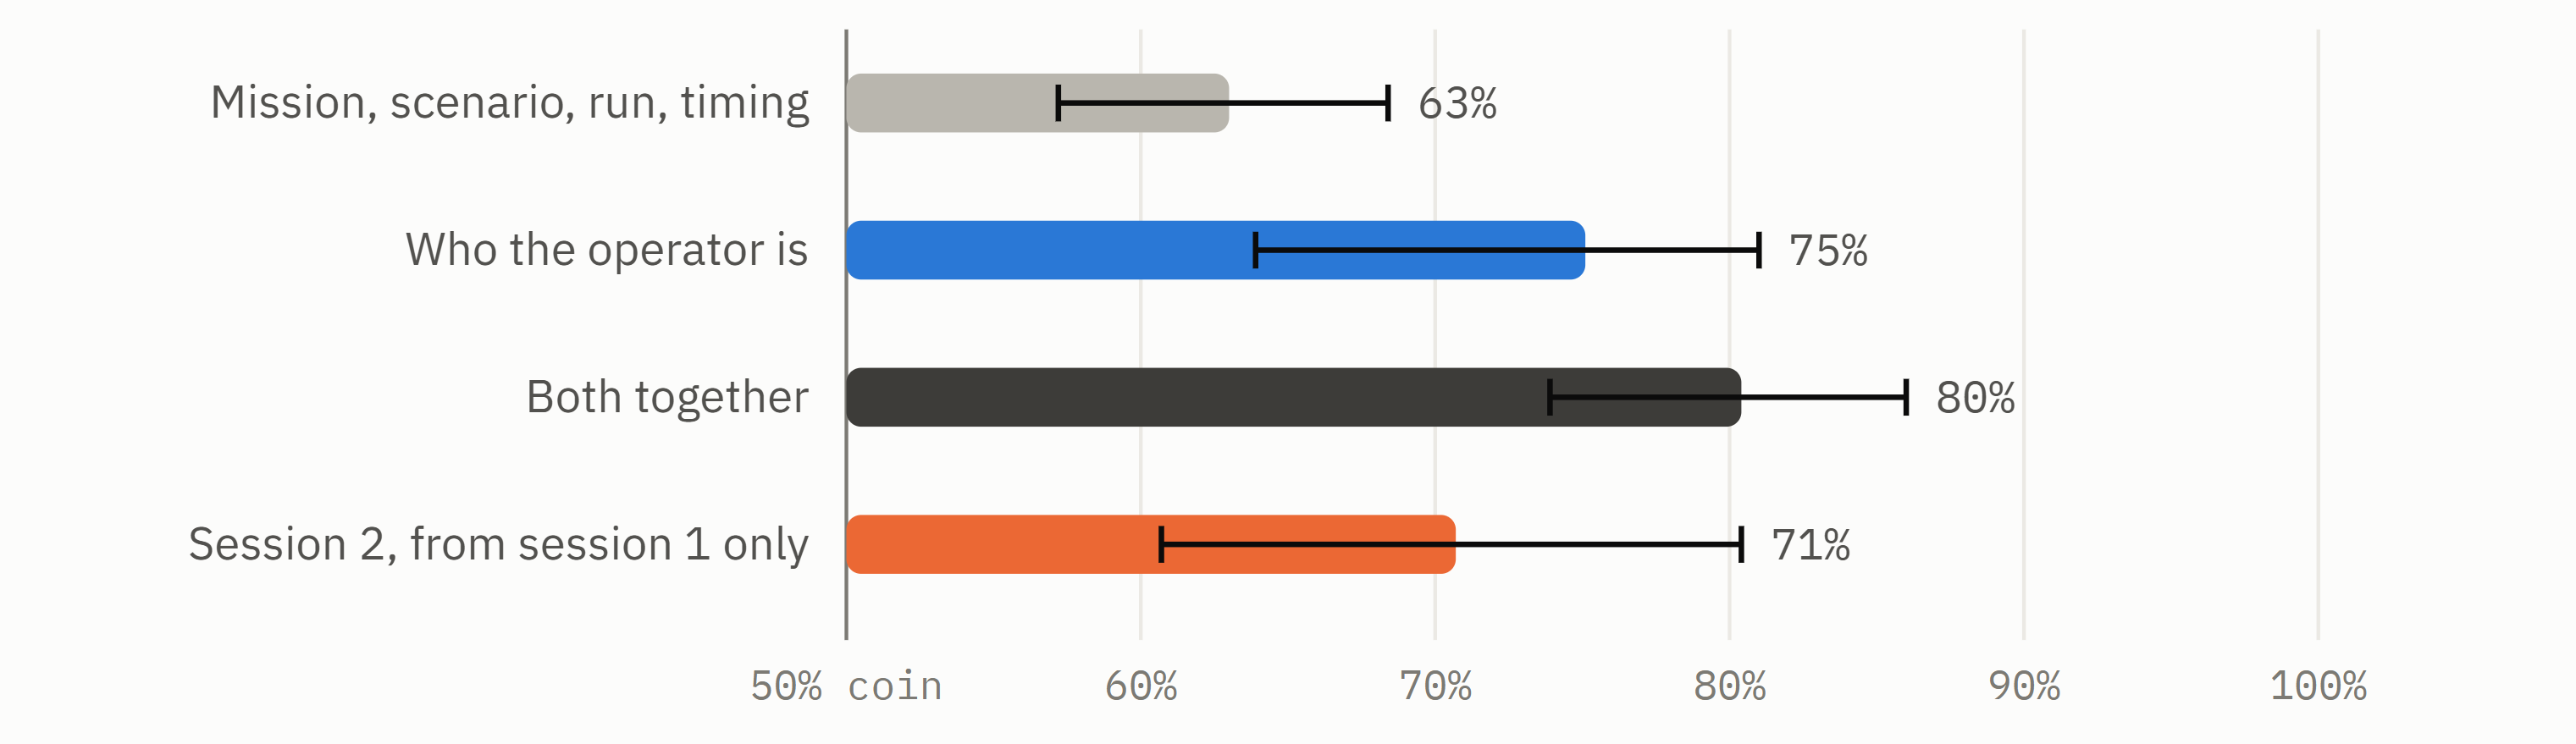
\includegraphics[width=\linewidth,height=0.23\textheight,keepaspectratio]{figs/results/f-personal-style__who-vs-what__auc.png}
\caption{The same comparison as a ranking test (AUC); whiskers are 95\% intervals (people resampled).}
\label{fig:res:personal-style:who-vs-what:auc}
\end{subfigure}
\par\smallskip
\caption{\textbf{Who decides matters more than what is being decided}}
\label{fig:res:personal-style:who-vs-what}
\end{figure}

\paragraph*{Key numbers.}

\begin{itemize}[leftmargin=1.2em,itemsep=1pt]

\item Pseudo-R$^2$: mission + timing 4\%; person 24\%; both 30\%

\item Card uptake per person 8\%--100\%, median 61\%; 6 people $\geq$ 90\%, 3 people $\leq$ 25\%

\item Telling a taken from a not-taken decision (AUC): mission and timing 63\% [57\%, 68\%]; the person, from their other decisions, 75\% [64\%, 81\%]; both 80\% [74\%, 86\%]; session-2 decisions from the session-1 rate alone 71\% [61\%, 80\%] (321 decisions).

\item Right-or-wrong guessing: always 'card' 66\%; mission 65\%; person 70\%; both 77\%.

\item Person-only pseudo-R$^2$ with the person labels shuffled: 4\% on average (95th percentile 6\%), against 24\% observed.

\end{itemize}

\paragraph*{Method.} {\small 606 strategic decisions. Three logistic models of ``card taken'': (a) mission and timing only --- drone types needed, drones needed, scenario, session 1 or 2, decision number; (b) the person only (one term each); (c) both. McFadden pseudo-R$^2$ = how much each improves on predicting the overall rate for everyone (0 = no better, 1 = perfect). Descriptive, not a test: with \textasciitilde{}18 decisions each, the person-only model flatters itself a little; refitted 200 times with the person labels shuffled it scores 4\% on average, so about 20 of its 24 points are real. Retest of raw card uptake session 1 vs 2: $\rho$ = .57 (.62 once game-adjusted, next section). \textbf{In plain terms} (the second view): AUC = the chance a model ranks a random card-taken decision above a random not-taken one. The person enters as their rate on all their OTHER decisions (on the log-odds scale), so no decision predicts itself; 'session 2 from session 1' uses only each person's session-1 rate. Intervals: people resampled 1,000 times, predictions held fixed.}

\paragraph*{What participants said.} \regtext{People often described their use of the assistants as part of who they are: 'naturally conservative' (P32), 'I'm more conservative' (P26), 'I always let the agent do it first' (P13). At the extremes, P14 used the assistants 'for almost every allocation' and P16 'manually overrode most of the time'. Against this, several gave the situation as the reason: workload (P32, 9 of 33 coded C11), being resource-constrained (P22), mission size (C03). P32 calls themself 'naturally conservative' and also says their use was 'very much about workload', so a person's style and the situation are both in play.}

\clearpage

\subsubsection{How far each habit holds from one session to the next}\label{sec:res:personal-style:retest-summary}

\noindent \passtag{for the paper}

\noindent \regtext{One line per habit: how strongly a person's place on that habit in session 1 predicts their place in session 2 ($\rho$; 0 = no carry-over, 1 = same order of people). Six of the ten carry over clearly and survive correction for testing ten (coloured). Editing cards, going manual before the cards load and topping up drones on multi-type missions carry over weakly, and topping up drones on single-type missions does not carry over at all ($\rho$ $-$.09). ``Keeps the Suggest plan'' is high partly because 24 of 33 people kept every Suggest plan in both sessions.} (Figure~\ref{fig:res:personal-style:retest-summary})

\begin{figure}[H]
\centering
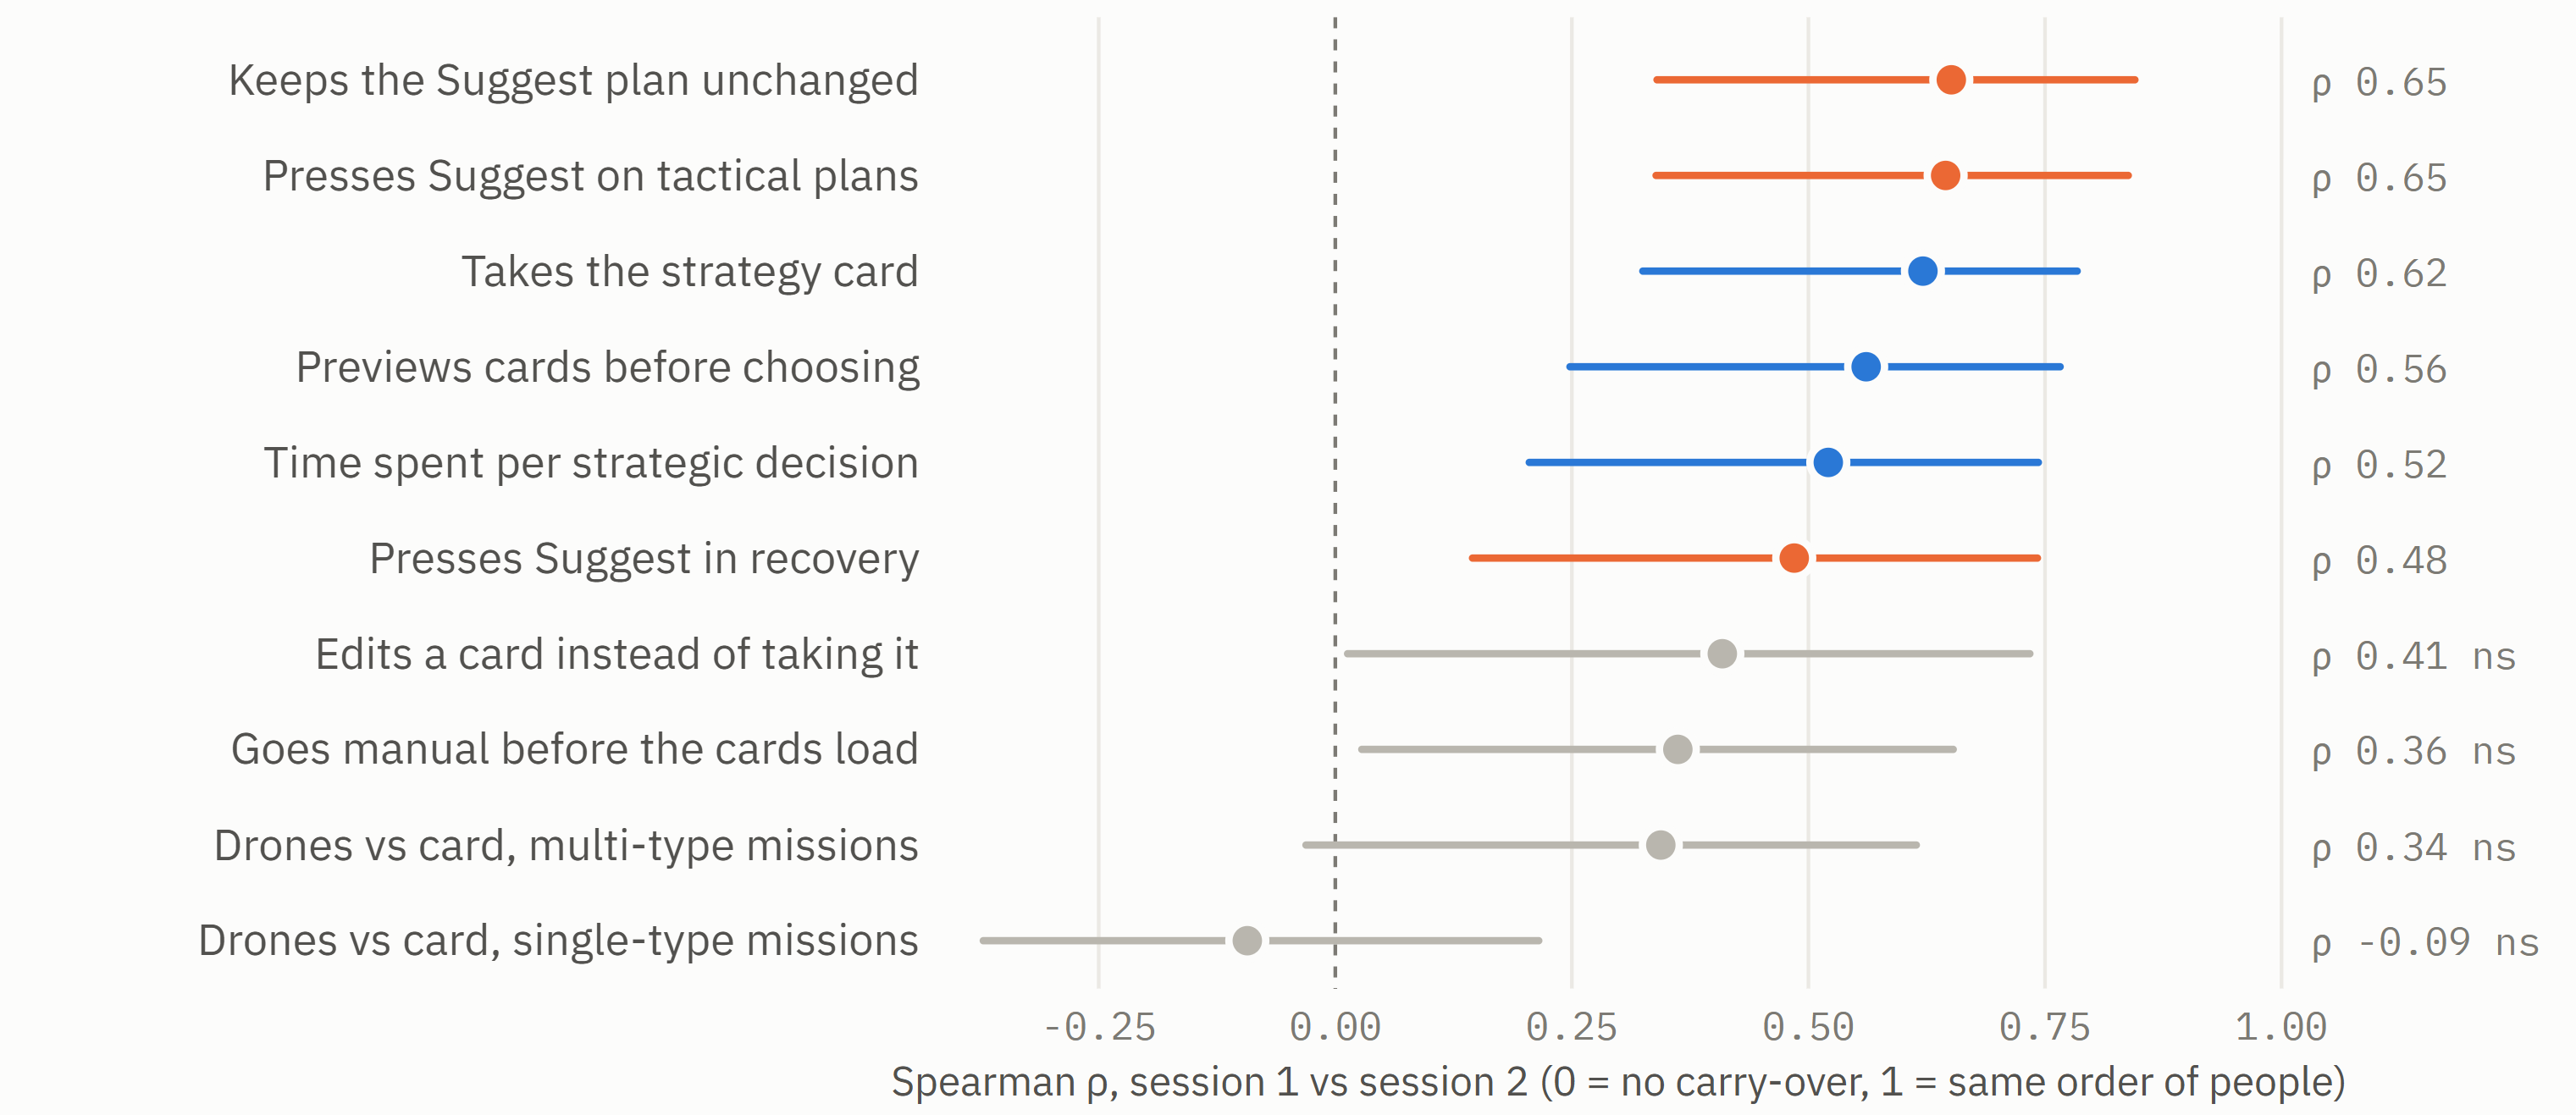
\includegraphics[width=\linewidth,height=0.55\textheight,keepaspectratio]{figs/results/f-personal-style__retest-summary__main.png}
\caption{\textbf{How far each habit holds from one session to the next}}
\label{fig:res:personal-style:retest-summary}
\end{figure}

\paragraph*{Method.} {\small 33 people. For each habit, Spearman $\rho$ between session-1 and session-2 values, each first z-scored within the game played; 95\% intervals from resampling people 2000 times; Holm correction across the ten. The same $\rho$ values are the right-hand column of the habits chart in the first section.}

\paragraph*{What participants said.} \regtext{Some people say they kept their approach and some say they changed it. P18 'sort of changed from the first one' (led) and P30 'used more personalized' in session 2. Four people describe a real shift in the think-aloud: P06 and P31 came to rely on the assistants more and check less, while P35 and P15 went back to deciding for themselves after the strategy cards made errors. That fits habits that carry over clearly but not completely.}

\clearpage

\subsubsection{Strategic and tactical reliance go together only loosely between people}\label{sec:res:personal-style:axis-scatter}

\noindent \passtag{for the paper}

\noindent \regtext{Each dot is a person: x = share of strategy cards taken, y = share of tactical plans where Suggest was pressed. Between people the two are only weakly linked ($\rho$ = .37, and .33 once each is measured against others who played the same game): plenty of people press Suggest on almost every plan while taking only half the cards, so knowing how much someone relies on one assistant tells you little about the other. Part of the reason is a ceiling: Suggest is pressed on a median 86\% of plans. The second view asks a different question: when the \emph{same} person takes more cards in one session than the other, do they also press Suggest more? Yes ($\rho$ = .51). So use of the assistants is not one fixed trait spanning both tiers, but within a person there is a session-level ``leaning on the assistants today'' that moves both together.} (Figure~\ref{fig:res:personal-style:axis-scatter})

\begin{figure}[H]
\centering
\begin{subfigure}[t]{\linewidth}
\centering
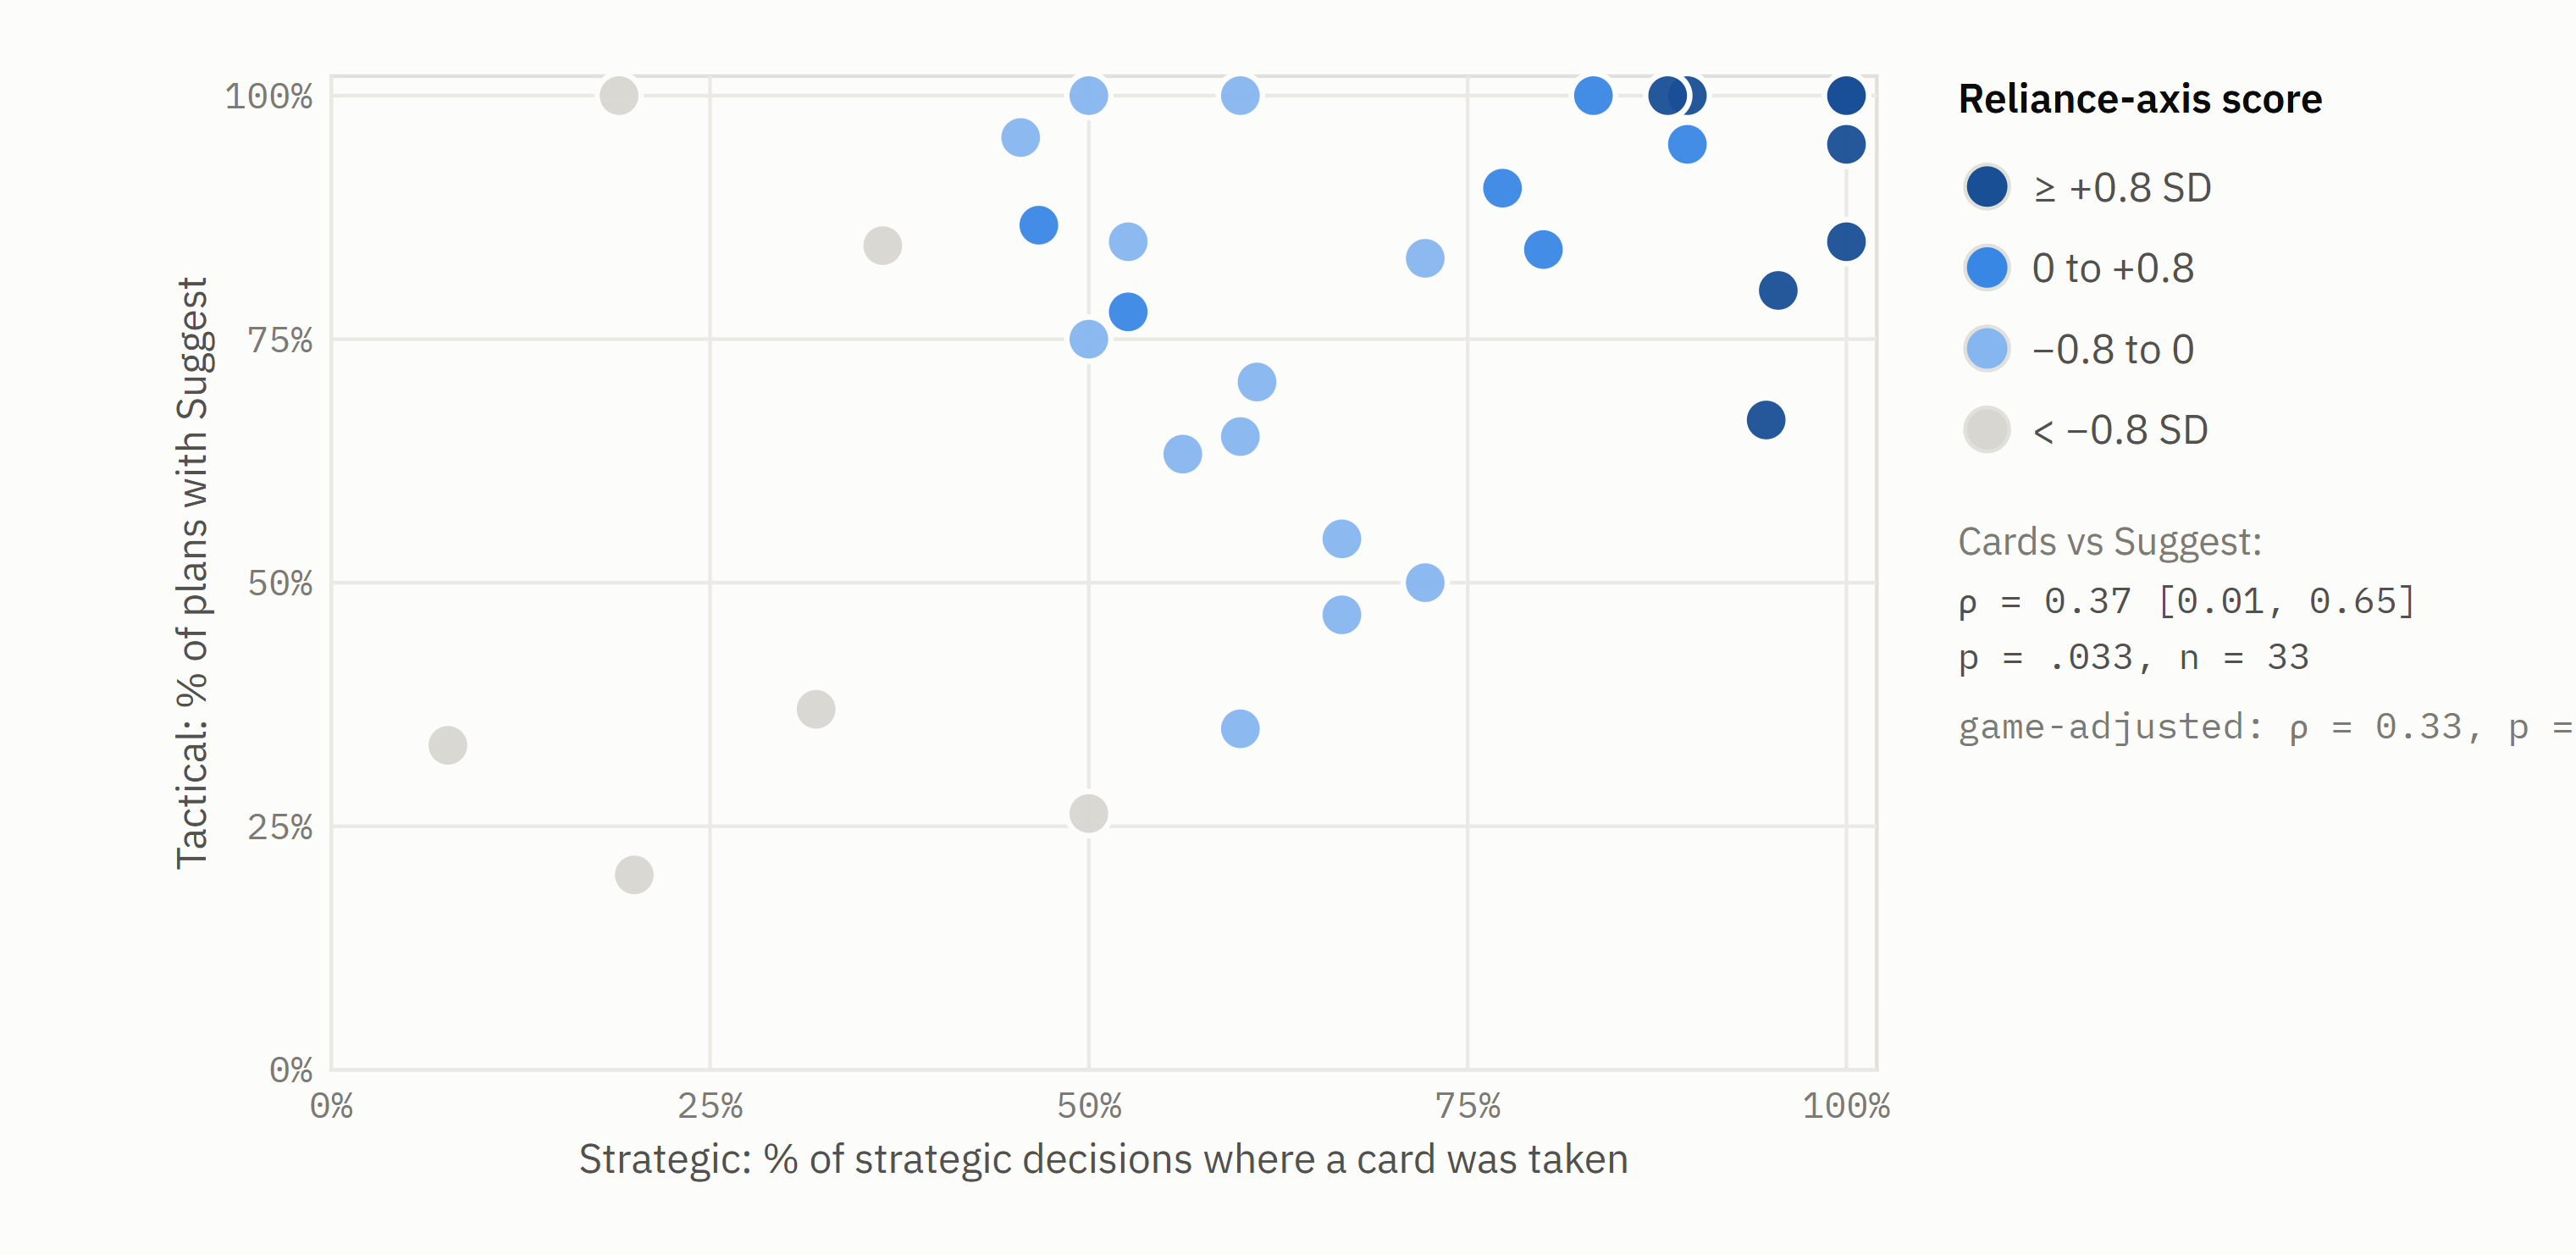
\includegraphics[width=\linewidth,height=0.23\textheight,keepaspectratio]{figs/results/f-personal-style__axis-scatter__between.png}
\caption{Between people.}
\label{fig:res:personal-style:axis-scatter:between}
\end{subfigure}
\par\smallskip
\begin{subfigure}[t]{\linewidth}
\centering
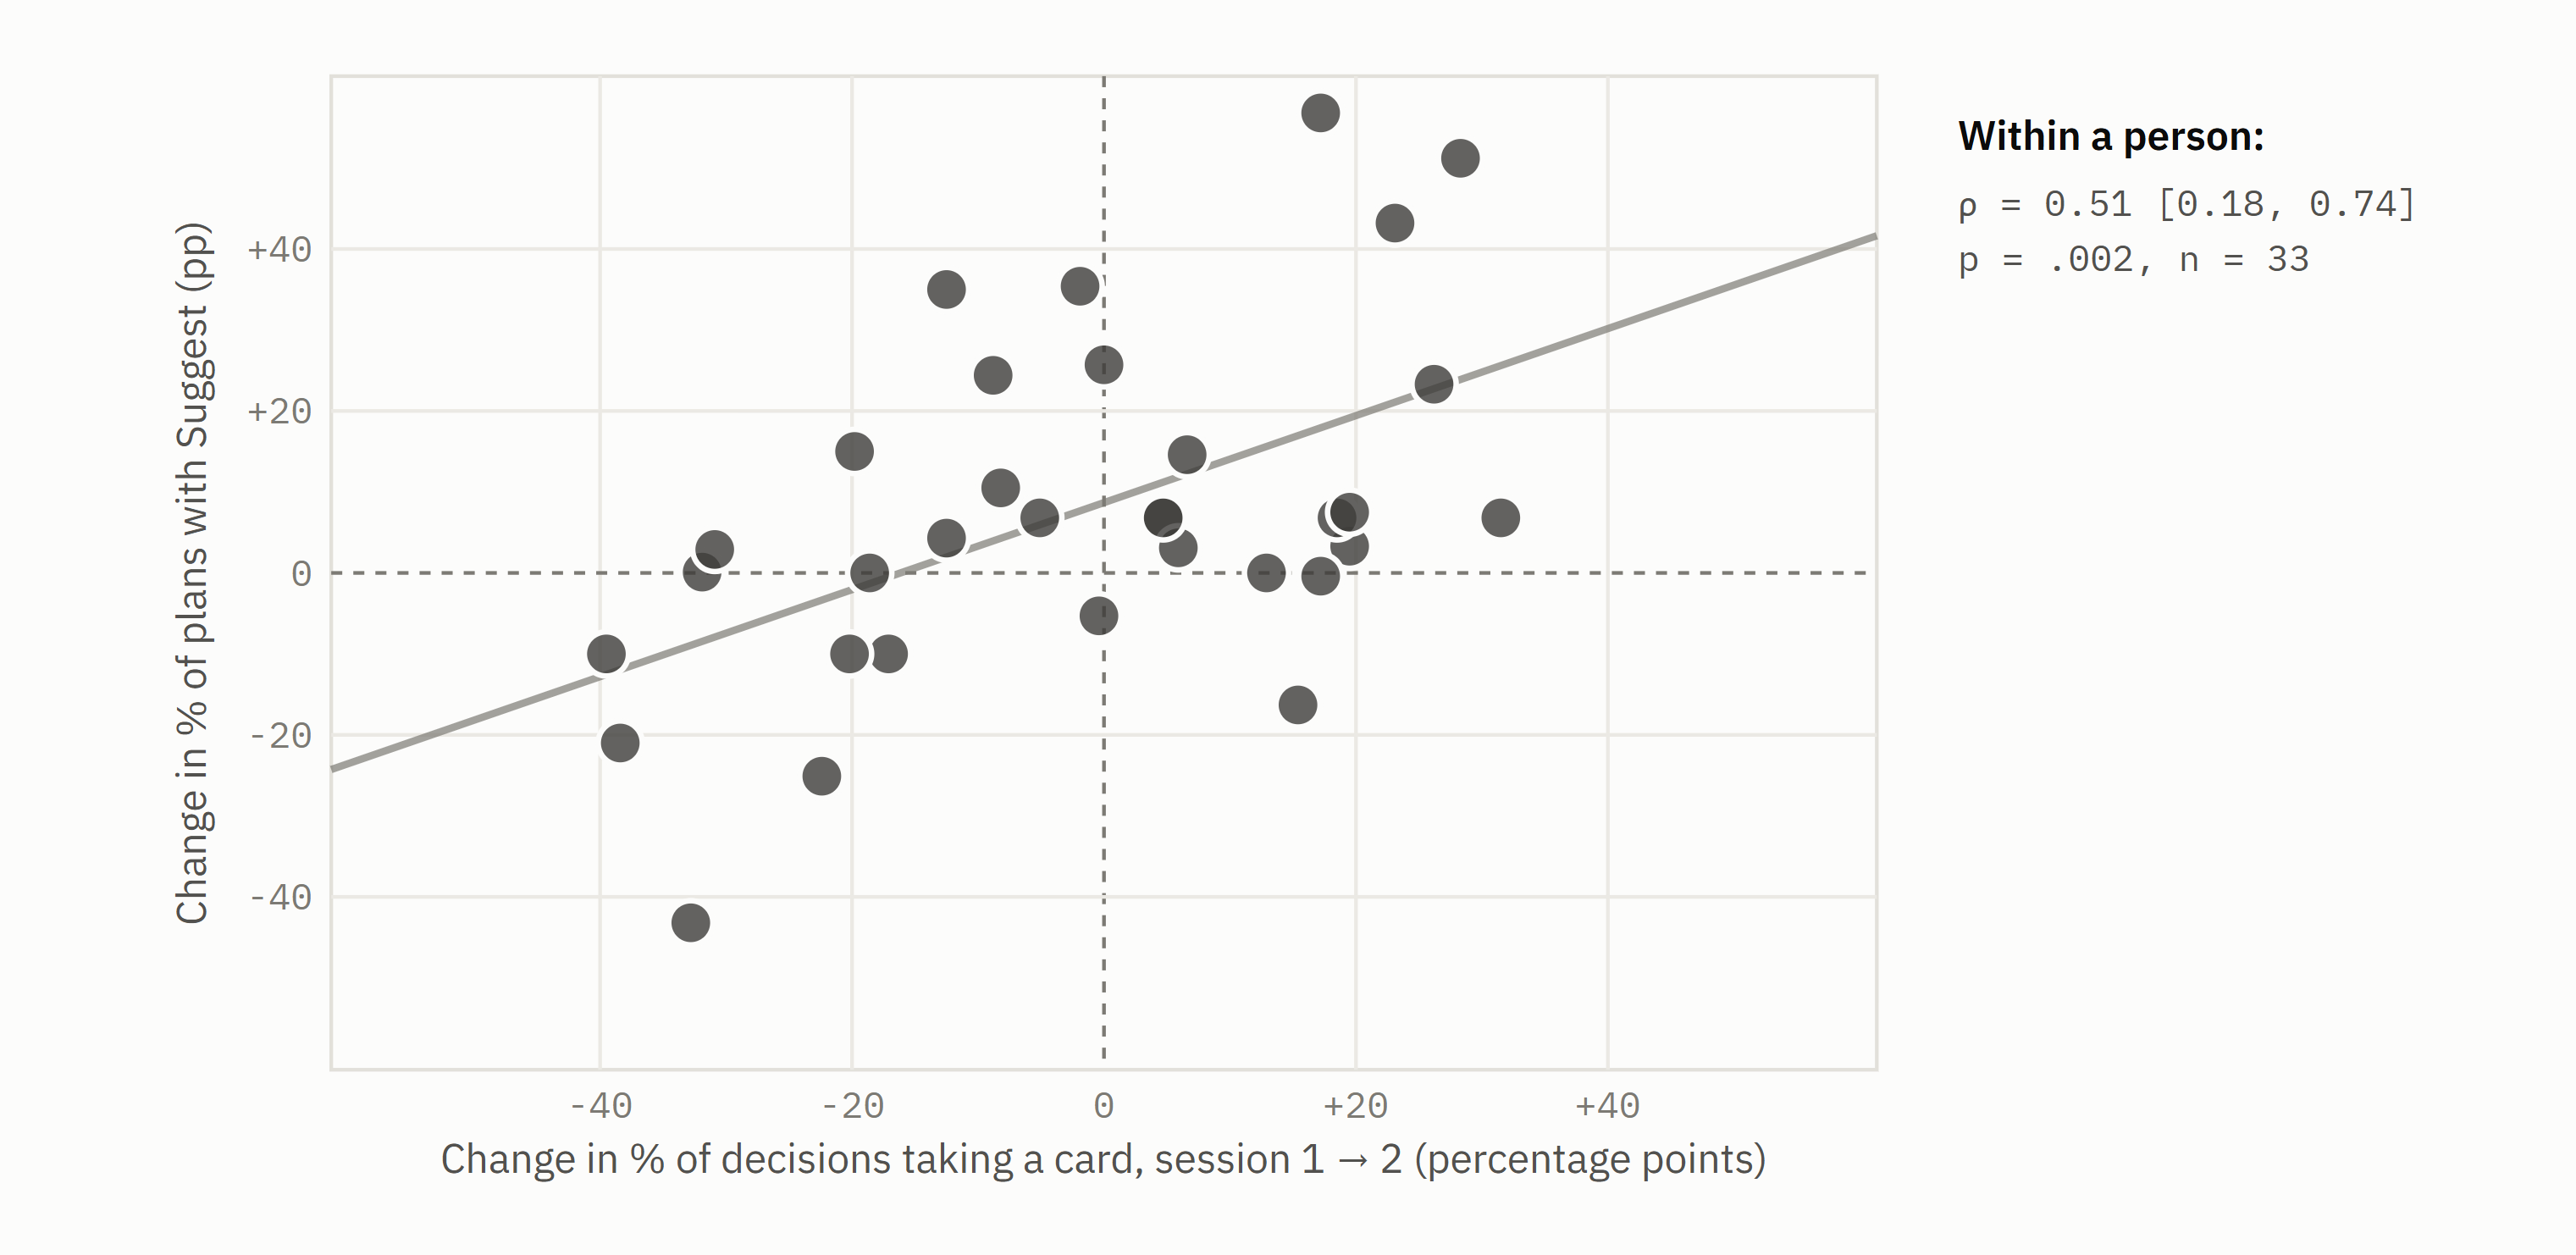
\includegraphics[width=\linewidth,height=0.23\textheight,keepaspectratio]{figs/results/f-personal-style__axis-scatter__within.png}
\caption{Within a person: change from session 1 to session 2.}
\label{fig:res:personal-style:axis-scatter:within}
\end{subfigure}
\par\smallskip
\caption{\textbf{Strategic and tactical reliance go together only loosely between people}}
\label{fig:res:personal-style:axis-scatter}
\end{figure}

\paragraph*{Key numbers.}

\begin{itemize}[leftmargin=1.2em,itemsep=1pt]

\item Between people, card uptake vs Suggest use: $\rho$ = .37 [.01, .65], p = .033 (raw); $\rho$ = .33 [$-$.03, .62], p = .058 (game-adjusted)

\item Within a person, change in card uptake vs change in Suggest use, session 1 $\rightarrow$ 2: $\rho$ = .51 [.18, .74], p = .002

\item Card uptake vs Suggest in recovery: $\rho$ = .42, p = .014; vs keeping the Suggest plan unchanged: $\rho$ = .20, p = .26

\item Card taking and previewing: $\rho$ = .79 (largely mechanical: choosing a card means clicking it)

\end{itemize}

\paragraph*{Method.} {\small Between people: one value per person, both sessions pooled (n = 33), Spearman $\rho$ with a Fisher interval; the game-adjusted version first subtracts the mean of everyone who played the same game from each session, then averages the person's two sessions. Within a person: the session-2 minus session-1 change in card uptake against the change in Suggest use, both game-adjusted (n = 33). Checked: the within-person link holds without game adjustment ($\rho$ = .56), and points the same way whichever scenario came first ($\rho$ = .47, p = .058 with Strategic Heavy first, n = 17; $\rho$ = .63, p = .010 with Tactical Heavy first, n = 16).}

\paragraph*{What participants said.} \regtext{Many describe relying on the two assistants differently, which fits the loose link between people. The most common split is to keep the strategic decision and hand over the tactical one: P22, P28, P30 and P32 say so, and P14 checked the tactical tier harder. A few did the reverse: P11 said they would use the strategic one more and built small plans themself, and P16 overrode the cards but 'more or less fully relied' on Suggest. P10 describes the two moving together: taking the Aggressive card makes Suggest the obvious next step.}

\clearpage

\subsubsection{Individual, not types}\label{sec:res:personal-style:not-types}

\noindent \passtag{numbers only}

\noindent \regtext{Distinct people, but not distinct kinds of people. If there were types (say ``delegators'' and ``hand-builders''), people would sit in clumps with gaps between them, and splitting them into groups would find clean, well-separated groups. Three plain checks say they do not. \textbf{(1) The map:} placed by their two biggest habit dimensions, the 33 operators form one continuous cloud; it looks just like 33 simulated operators that have no types by construction, and the best two-group split simply cuts the cloud in half. \textbf{(2) Separation:} however many groups we ask for (2, 3 or 4), the real people separate no better than the no-types simulations do, and every value is below the usual threshold for real group structure. \textbf{(3) Recurrence:} grouping each session separately, the same people barely end up together twice, no more than in a smooth cloud where people keep their place. The archetype names (Delegator, Deliberate builder, Fast tinkerer) are best kept as labels for the ends of the main dimensions.} (Figure~\ref{fig:res:personal-style:not-types})

\begin{figure}[H]
\centering
\begin{subfigure}[t]{0.495\linewidth}
\centering
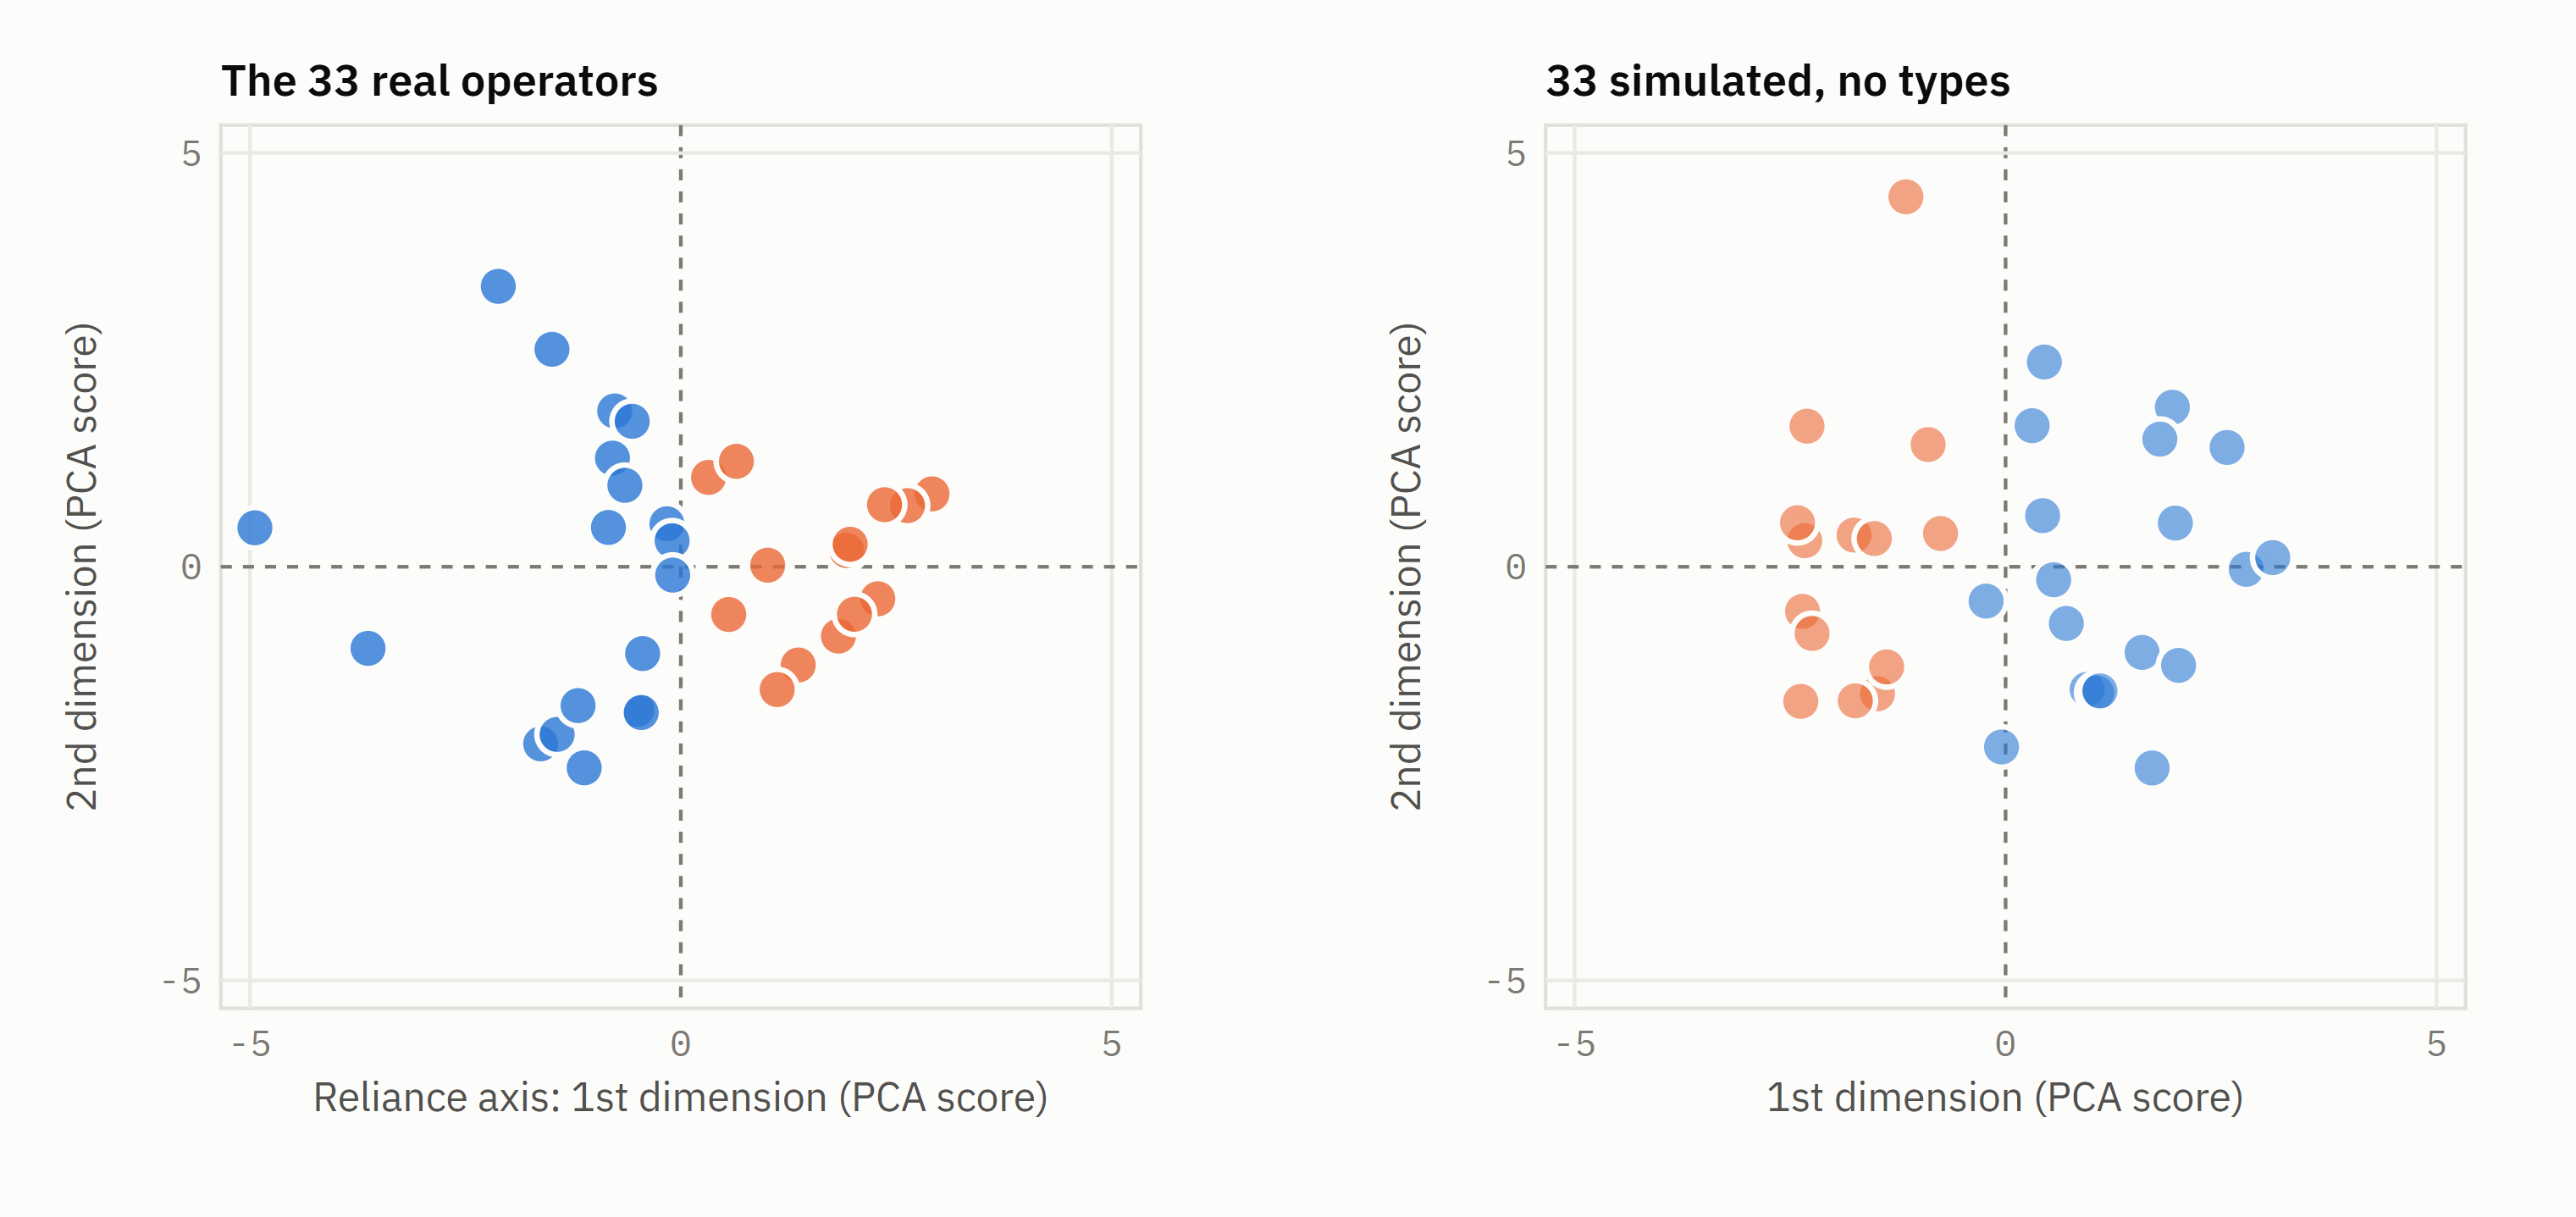
\includegraphics[width=\linewidth,height=0.23\textheight,keepaspectratio]{figs/results/f-personal-style__not-types__map.png}
\caption{The people, mapped on the first two principal components.}
\label{fig:res:personal-style:not-types:map}
\end{subfigure}
\hfill
\begin{subfigure}[t]{0.495\linewidth}
\centering
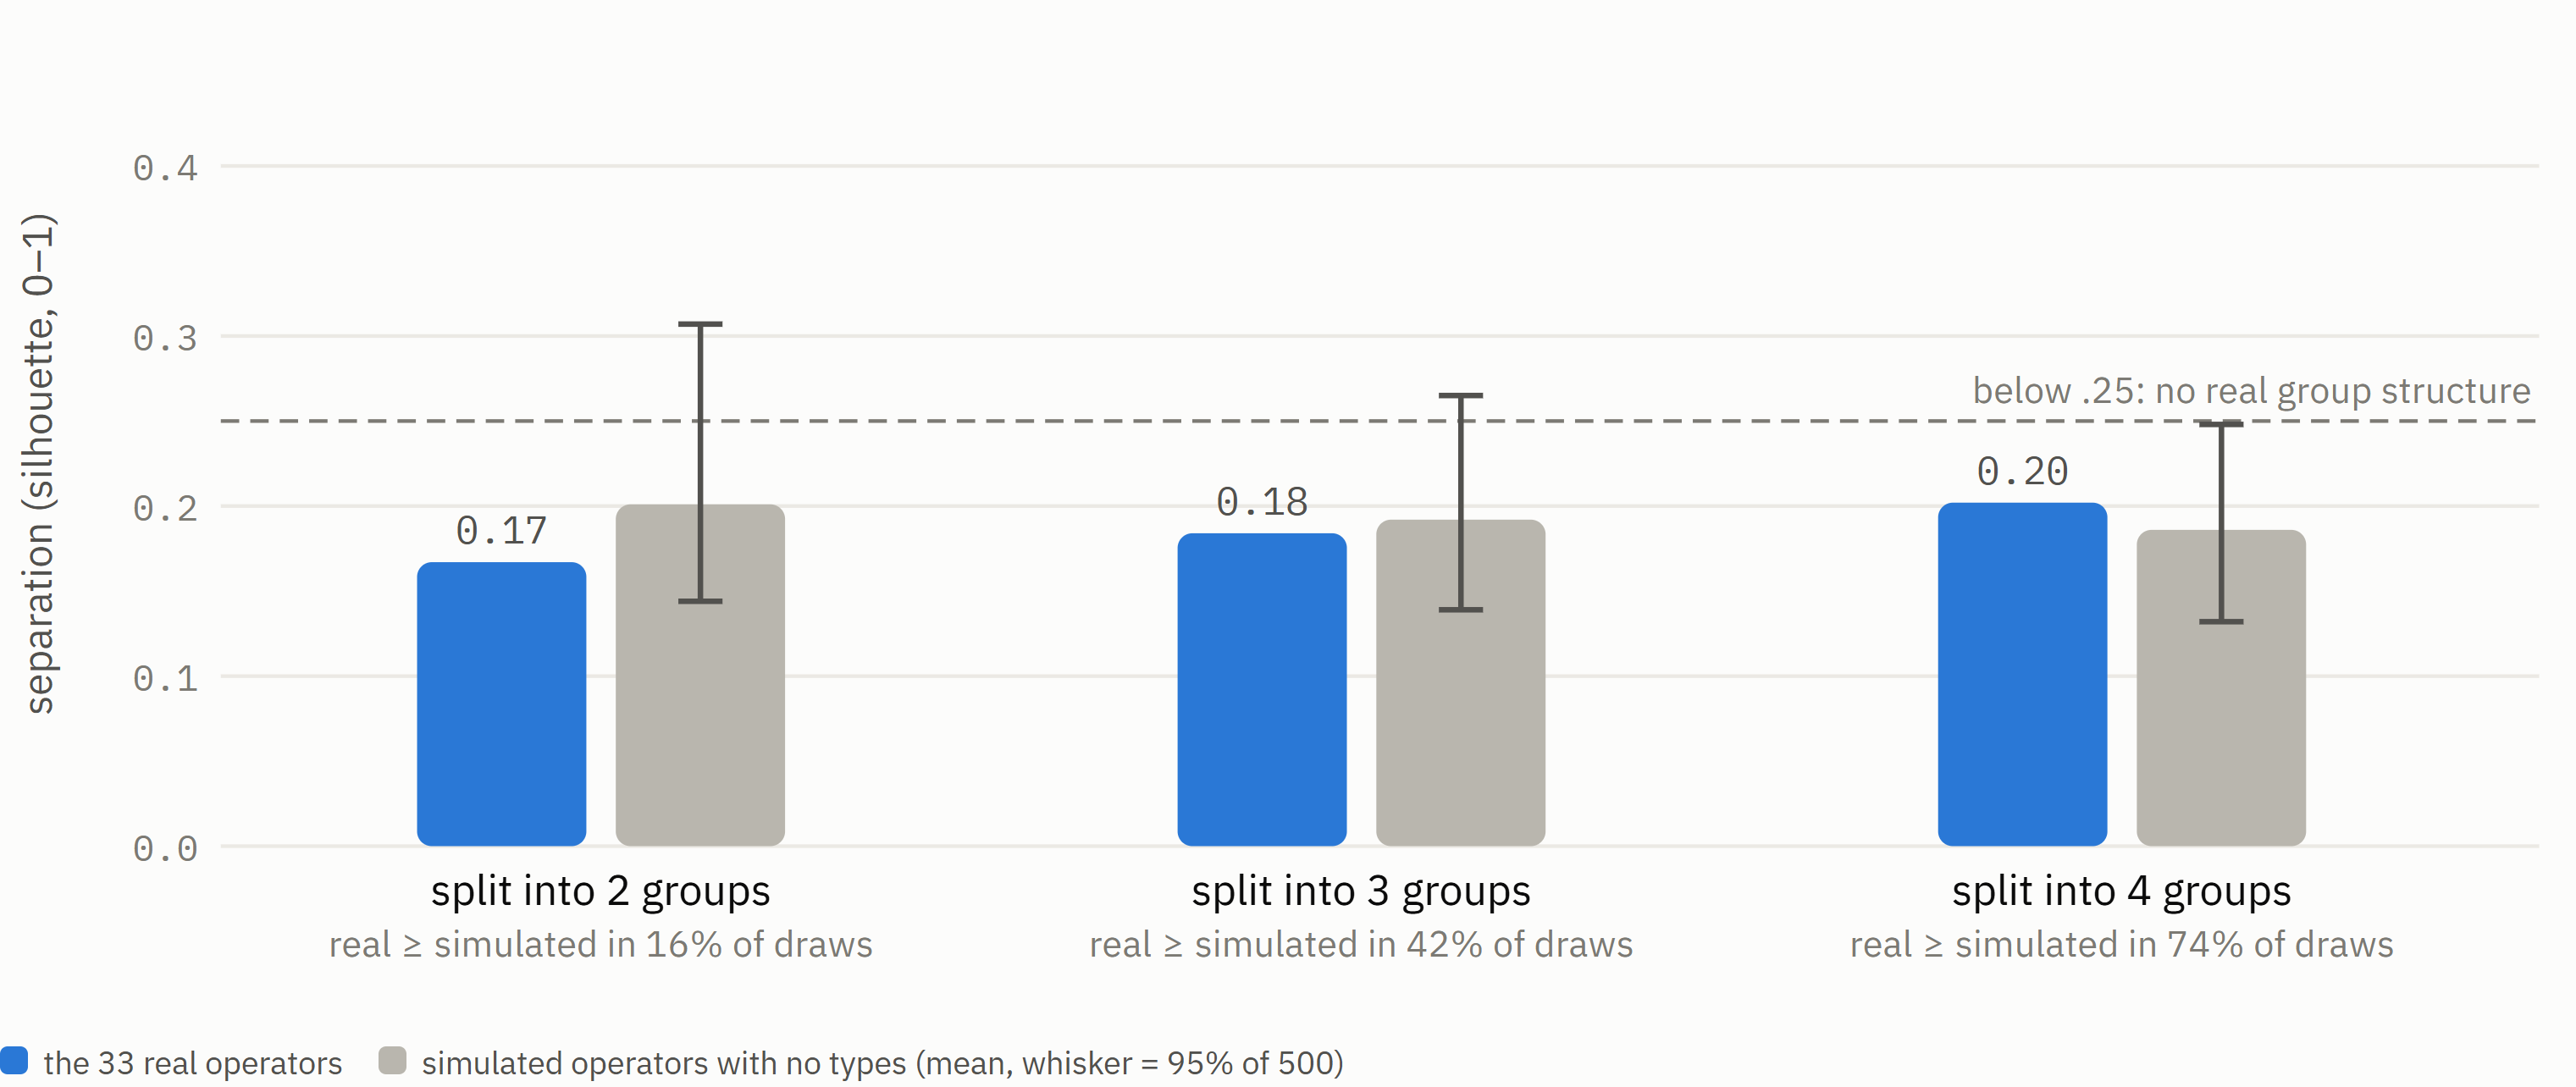
\includegraphics[width=\linewidth,height=0.23\textheight,keepaspectratio]{figs/results/f-personal-style__not-types__separate.png}
\caption{Cluster separation (silhouette) against no-types simulations.}
\label{fig:res:personal-style:not-types:separate}
\end{subfigure}
\par\smallskip
\begin{subfigure}[t]{0.495\linewidth}
\centering
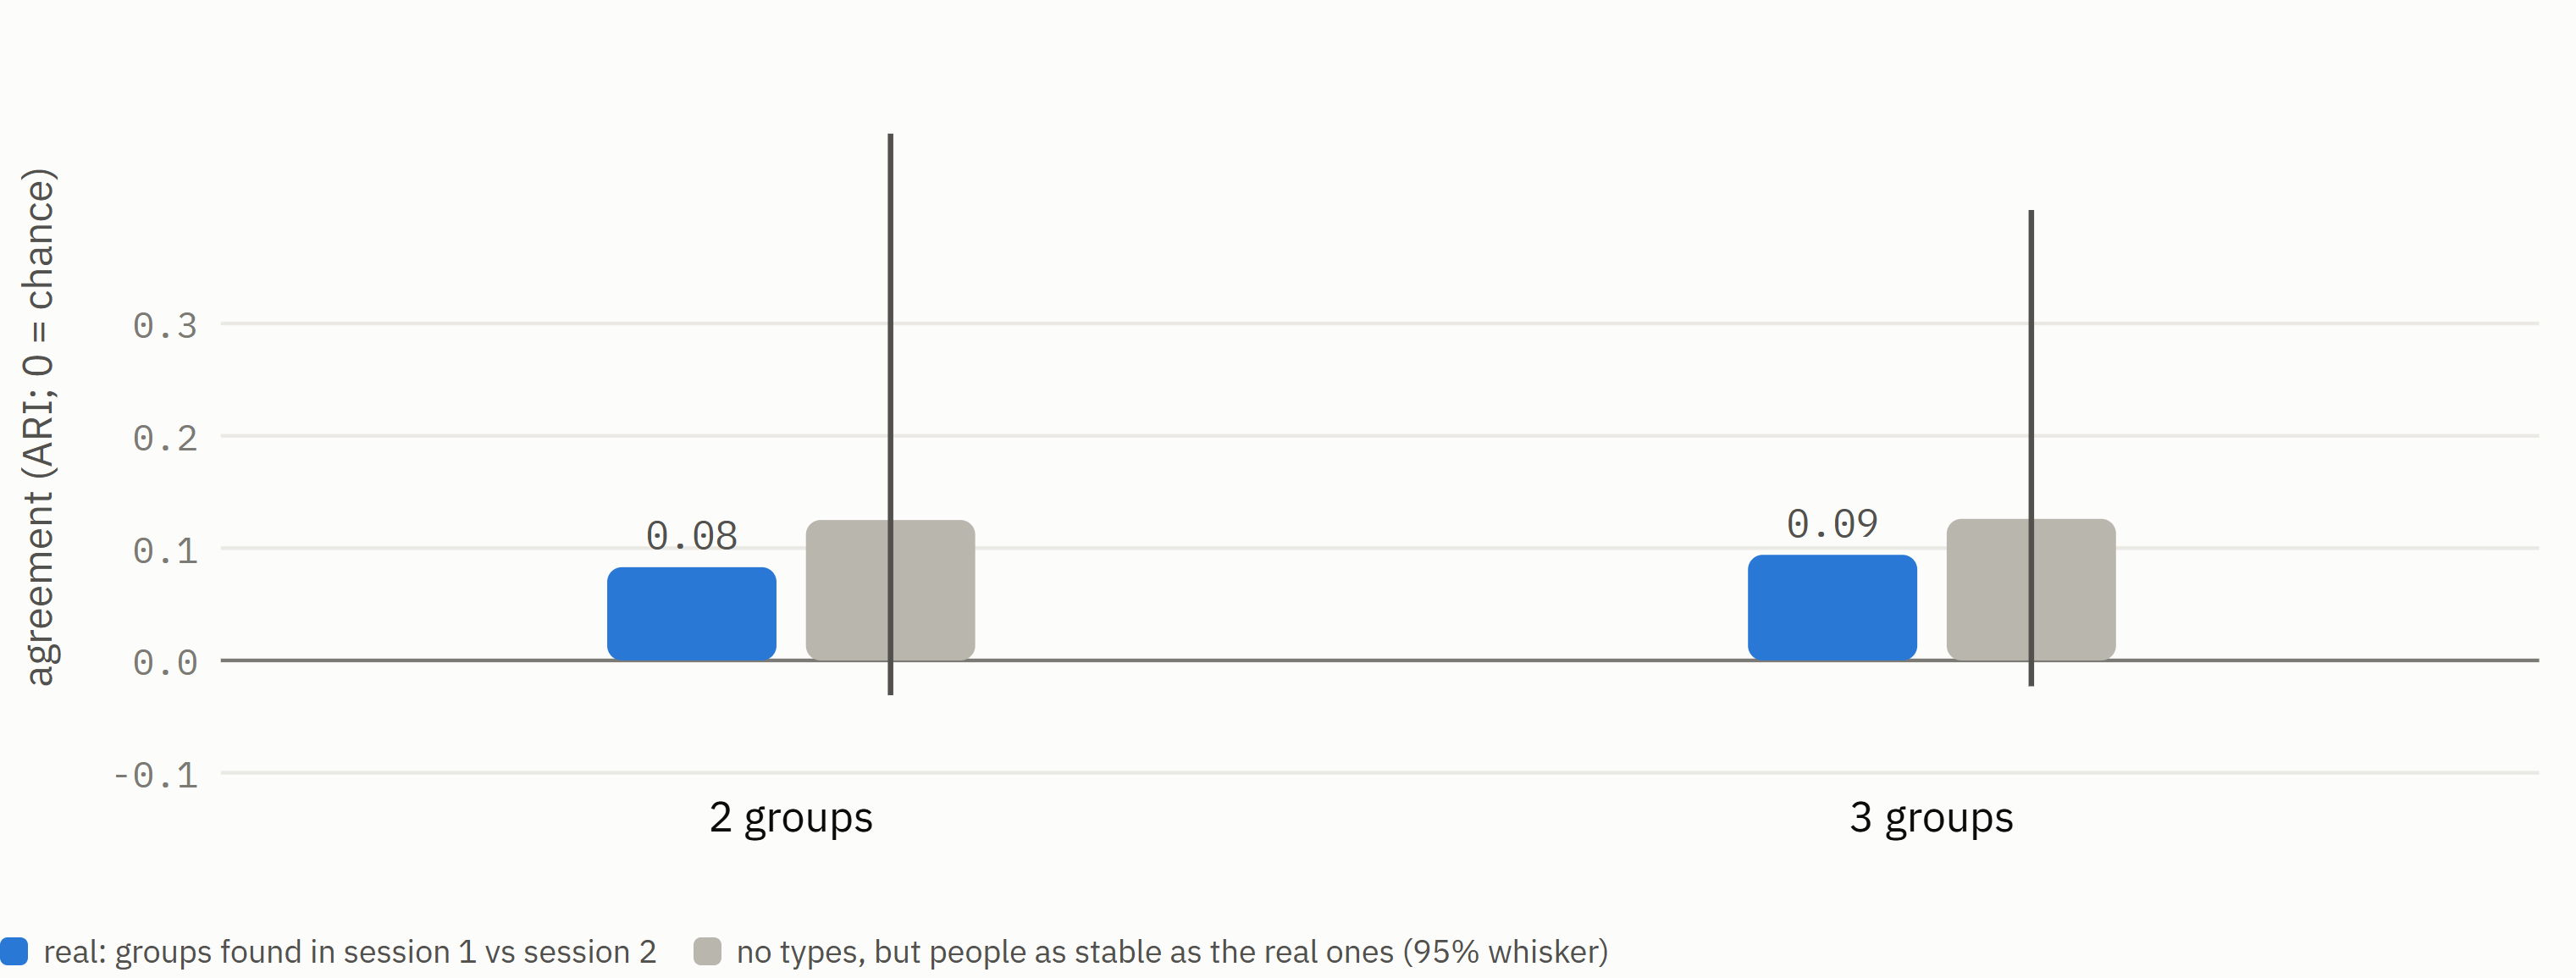
\includegraphics[width=\linewidth,height=0.23\textheight,keepaspectratio]{figs/results/f-personal-style__not-types__recur.png}
\caption{Recurrence of groupings across sessions (adjusted Rand index).}
\label{fig:res:personal-style:not-types:recur}
\end{subfigure}
\hfill
\caption{\textbf{Individual, not types}}
\label{fig:res:personal-style:not-types}
\end{figure}

\paragraph*{Key numbers.}

\begin{itemize}[leftmargin=1.2em,itemsep=1pt]

\item Separation (silhouette), real vs no-types simulations: 2 groups .17 vs .20 [.14, .31]; 3 groups .18 vs .19 [.14, .27]; 4 groups .20 vs .19 [.13, .25]; a no-types sample separates at least as well 84\%, 58\% and 26\% of the time

\item Groups in session 1 vs session 2 (ARI): 2 groups .08, 3 groups .09; a stable no-types cloud gives .13 on average (95\% of simulations $-$.03 to .47 for 2 groups, $-$.02 to .40 for 3), at least as high as the real value about 55\% of the time; shuffled labels give up to .12--.13

\item Round 1: two groups vs one, $\Delta$BIC 1.9 (needed > 10; 42\% of no-type simulations did at least as well)

\item Archetypes (extras2): three explain 46\% vs 43--59\% in the no-types continuum (p = .83); same archetype both sessions 61\% vs 30--79\% (p = .32)

\end{itemize}

\paragraph*{Method.} {\small Rows: the 33 people, each described by the ten habits pooled over both sessions and standardised. Grouping = k-means (the computer splits people into k groups so that each sits as close as possible to its group's centre; best of 20 starts). Separation = silhouette: for each person, how much closer they are to their own group than to the nearest other group, averaged (1 = tight clumps far apart; 0 = boundaries arbitrary; below .25 is conventionally ``no substantial structure'', Kaufman \&amp; Rousseeuw). Benchmark = 500 simulated samples of 33 operators drawn from one smooth cloud with the same distribution of each habit and the same correlations between habits as the real people, so they have no types by construction. (We use these rather than simply shuffling each habit, because shuffling also destroys the links between habits, and a cloud of linked habits separates slightly better than shuffled data without having any types: shuffled data give about .14.) Recurrence: each session's profiles (z-scored within game) are grouped separately and compared with the adjusted Rand index (1 = the same groupings, 0 = chance), against (a) shuffled labels and (b) 500 simulated pairs of sessions with no types but the same session-to-session stability of every habit as the real people. The map uses the first two principal components (50\% of the differences). Round 1's pre-registered test (mixture models compared by BIC) and the archetype simulations (extras2) reach the same conclusion; their numbers are kept below.}

\paragraph*{What participants said.} \regtext{Nobody described themselves or others as a 'type' of operator. People talked about their own rules, and several, such as P29, were still unsure of them partway through a session ('I haven't actually decided ... which ones are best to handle myself').}

\clearpage

\subsubsection{Nothing measured beforehand predicts the style}\label{sec:res:personal-style:not-disposition}

\noindent \passtag{for the paper}

\noindent \regtext{Attitude to AI (AIAS-4), verification propensity, views on human authority over AI (delegation scale and its single items, including ``a human should make the final decision''), and prior experience: 40 tests against five behaviours. Three reach p < .05 before correction, and <b>none survives Holm correction for the 40 tests. Three nominal hits is what chance alone produces: shuffling which person's questionnaire goes with which person's behaviour gives 2.0 such hits on average, and 3 or more in a third of shuffles. This is ``no evidence'', not proof of no link: the sample could only have detected fairly strong correlations (|$\rho$| $\geq$ .48), and it is almost uniformly AI-positive (AIAS-4 averages 8.0 / 10) and from computing or engineering (32 of 33). Within this sample, the large differences in style are not explained by what people say they think about AI.} (Figure~\ref{fig:res:personal-style:not-disposition})

\begin{figure}[H]
\centering
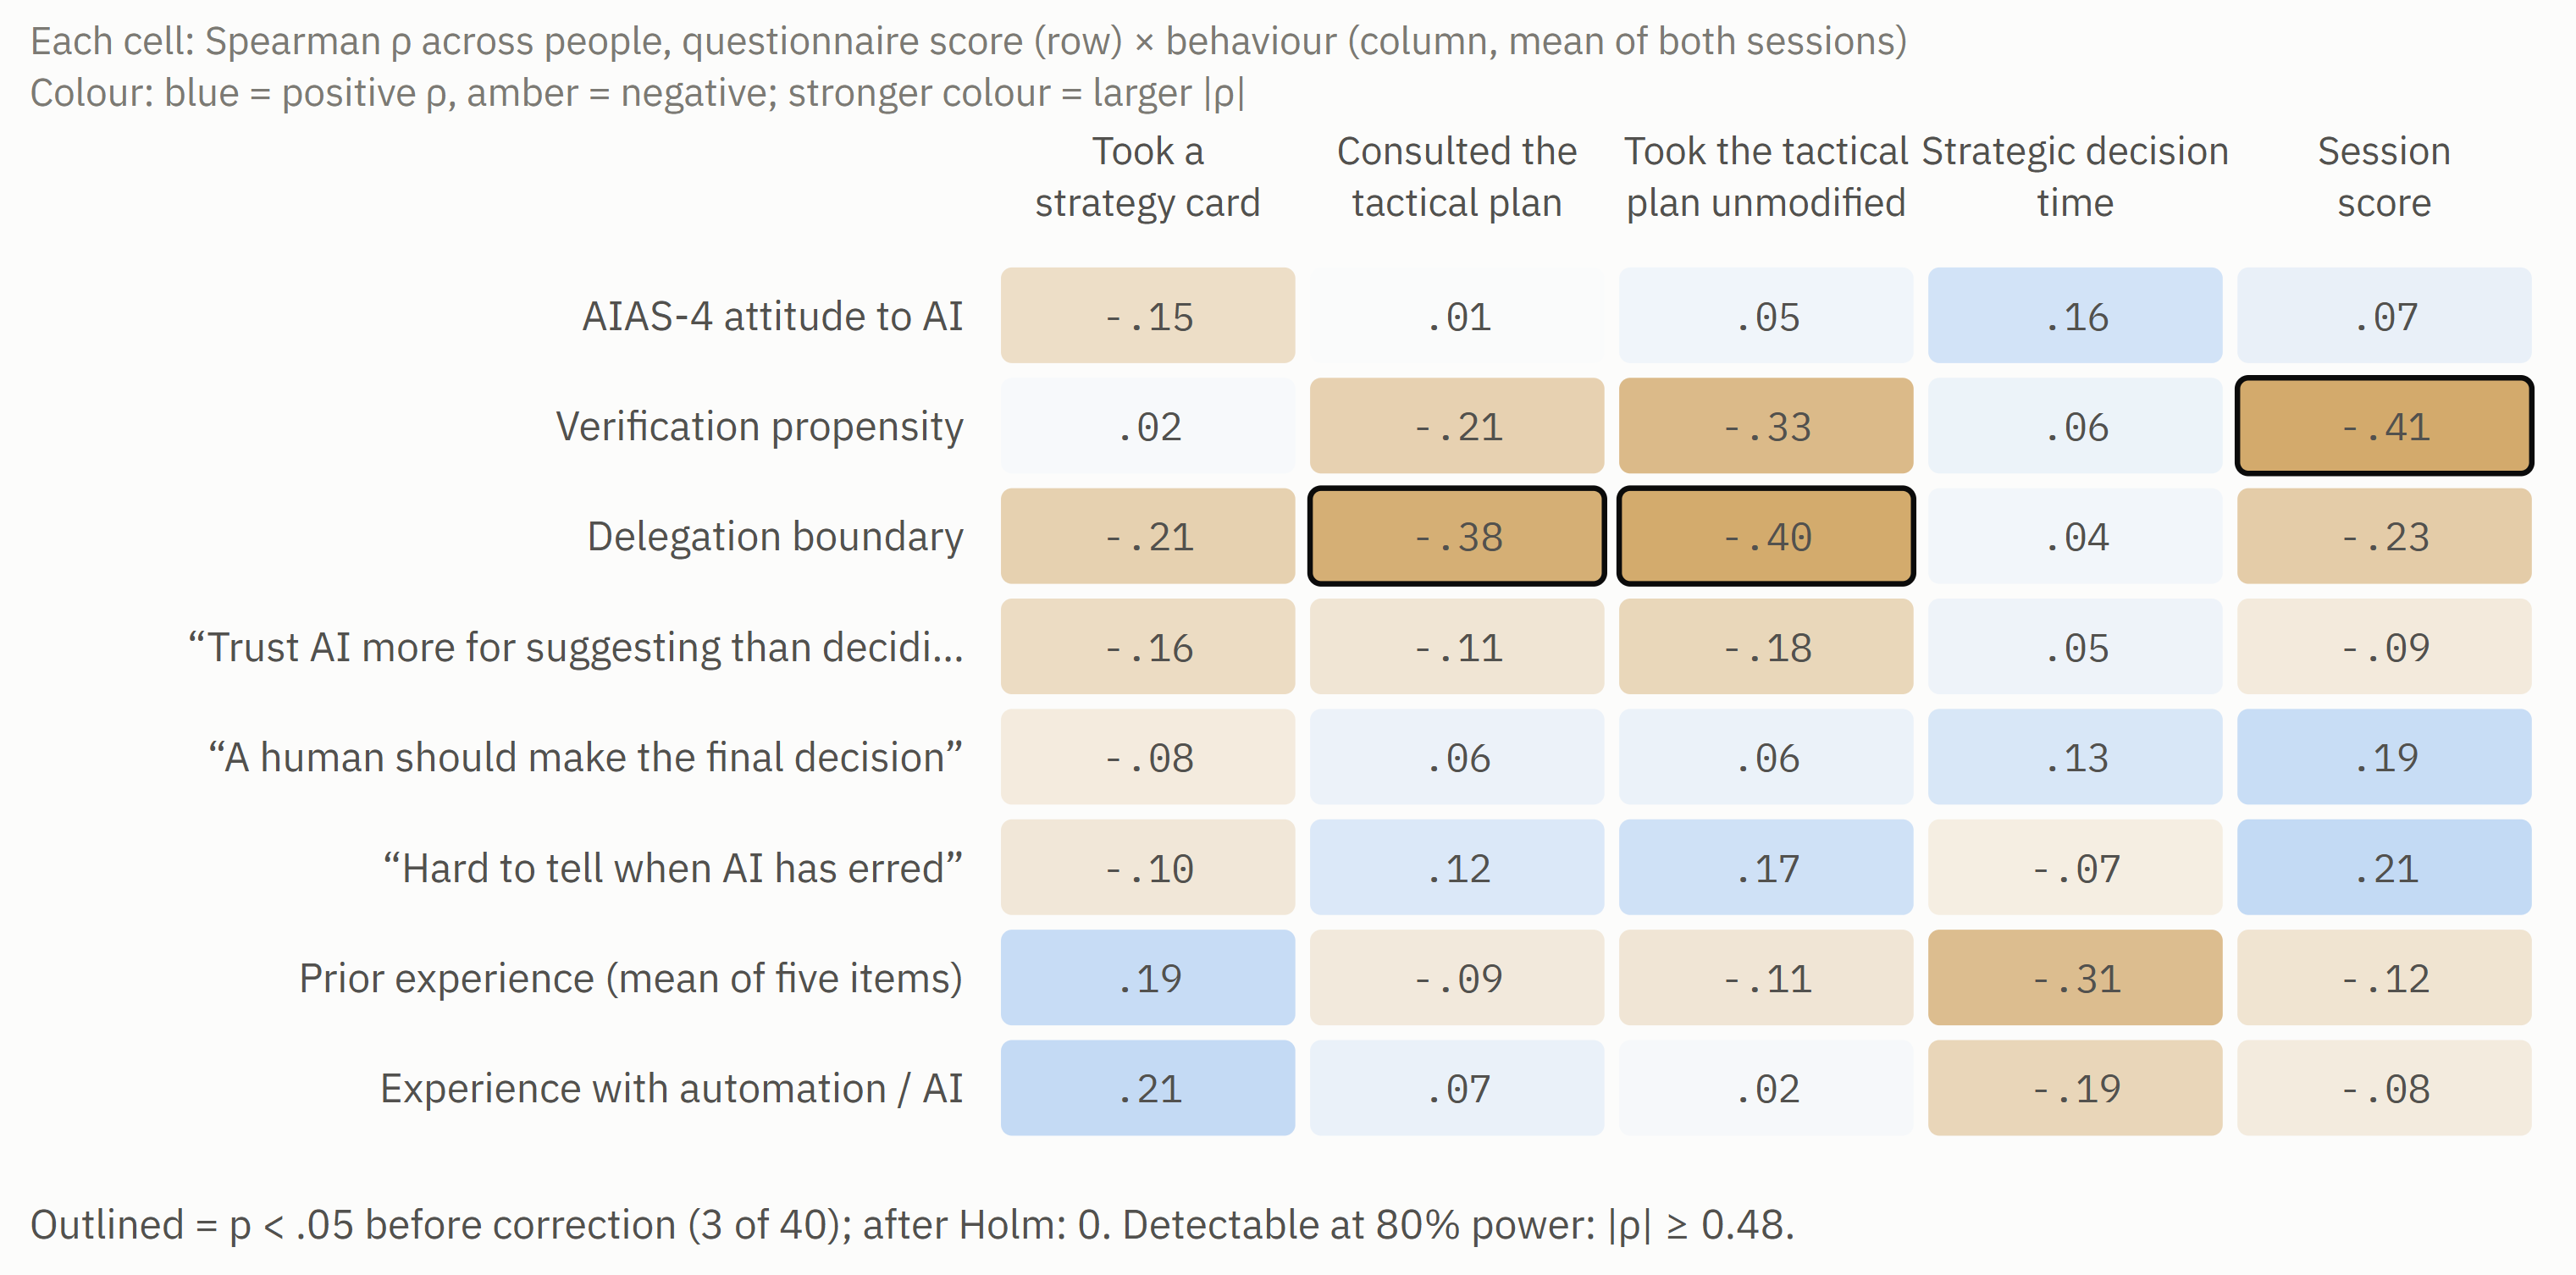
\includegraphics[width=\linewidth,height=0.55\textheight,keepaspectratio]{figs/results/f-personal-style__not-disposition__main.png}
\caption{\textbf{Nothing measured beforehand predicts the style}}
\label{fig:res:personal-style:not-disposition}
\end{figure}

\paragraph*{Key numbers.}

\begin{itemize}[leftmargin=1.2em,itemsep=1pt]

\item 0 of 40 tests survive Holm; 3 nominal (verification $\times$ score $\rho$ $-$.41; delegation $\times$ Suggest consulted $-$.38 and $\times$ plan kept $-$.40)

\item Chance alone gives 2.0 nominal hits on average; 3 or more in 34\% of 2000 shuffles of who-goes-with-whom; a p as small as the smallest one (.021) turns up somewhere in the grid in 51\% of shuffles

\item AIAS-4 $\times$ card uptake $\rho$ $-$.15; ``A human should make the final decision'' $\times$ card uptake $\rho$ $-$.08

\item AIAS-4 odds ratio for card taking 0.80 per SD [0.50, 1.27]; detectable only at about $\times$2

\item AIAS-4 mean 8.0 / 10 (SD 1.2); 32 of 33 from computing / engineering; detectable |$\rho$| $\geq$ .48

\end{itemize}

\paragraph*{Method.} {\small Per person: each questionnaire score (taken before session 1) against the average over both sessions of: card uptake, Suggest consulted, Suggest plan kept unmodified, strategic decision time, session score. Spearman $\rho$ per cell; Holm correction across all 40 together (build\_findings\_synthesis \texttt{analyse\_disposition}). Detectable effect = the correlation the sample had an 80\% chance to find at $\alpha$ = .05 (n = 32 with questionnaires). Round 1 H7's decision-level model gives the same answer for AIAS-4: odds of taking a card $\times$ 0.80 per SD [0.50, 1.27].}

\paragraph*{What participants said.} \regtext{When people talked about AI in general, it did not line up neatly with what they did. P04 does not trust the AI to be better than them but uses it because it is quicker. P24 says they really trust AI yet trims the cards to save drones. P15 calls the AI 'a little bit stupid' but hands it complex plans. P35 relies on it because they are 'not trained'. Most people explained their use by time pressure and job size rather than by a view about AI, which fits the null.}

\clearpage

\subsection{Small jobs by hand, big jobs to the assistant --- on both tiers, and it is where the assistant saves time}\label{sec:res:size-decides}

\regtext{\textbf{Summary.} The bigger the job, the more likely an operator hands it to an assistant, on both tiers. Measured the same way on both (drones the mission needs), the strategy card is taken on 56\% of the smallest missions vs 75\% of the largest, and Suggest is pressed on 54\% vs 91\%. Comparing each person only with themselves, every doubling of the mission multiplies the odds of handing over by about 1.6 (strategic) and 2.9 (tactical); 22 of 33 people hand over more on their biggest missions than their smallest on each tier. It survives every check we tried, including dropping the illogical Conservative cards and allowing for everyone having played the same missions. Three qualifications: on the strategic tier most of the effect is operators deciding small missions before the cards load; the strategic curve is lumpy (a dip at 5 drones, missions that mostly arrived in bursts in the Strategic Heavy games), so the dependable strategic contrast is one-type vs three-type missions; and handing over on one tier goes with handing over on the other (a mission allocated from a card gets Suggest at about twice the odds). The rule is sensible: the card is much quicker than building by hand on three-type missions and no quicker on one-type ones, and a Suggest plan is not slower: compared on missions of the same size it finishes about 15 s sooner, mostly because it is carried out faster.} \par\noindent{\small\textit{Strength of evidence (register rating): strong. Your verdict: core.}}

\subsubsection{Both tiers on one axis: the bigger the mission, the more it is handed over}\label{sec:res:size-decides:both}

\noindent \passtag{for the paper}

\noindent \regtext{For every mission, the share of decisions where the operator handed over (took a strategy card as offered, blue, or pressed Suggest in the tactical planner, orange) by how many drones the mission needs. Both rise. The tactical tier rises more steeply and keeps rising, from 54\% to 91\%. The strategic tier climbs from about half on small missions to about three quarters, with a dip at 5 drones. That dip is seven particular all-Fast missions, all in the two Strategic Heavy games, and six of them arrived in bursts: in one game two of them arrived 11 s apart in a run of seven missions inside one minute (minutes 1.6 to 2.6), in the other four of them arrived within 80 s (minutes 3.7 to 5.0) alongside three other missions. So by the time operators reached them 3--4 other missions were waiting, and they decided fast and often before the cards loaded. Busy arrival is likely part of it, but not all: missions of other sizes in the same bursts got the card more often (a 3-drone and a 6-drone mission in those bursts got it 67\% and 64\% of the time), and holding the queue fixed barely changes the 5-vs-3 comparison (see ``Why the 5-drone missions dip'').} (Figure~\ref{fig:res:size-decides:both})

\begin{figure}[H]
\centering
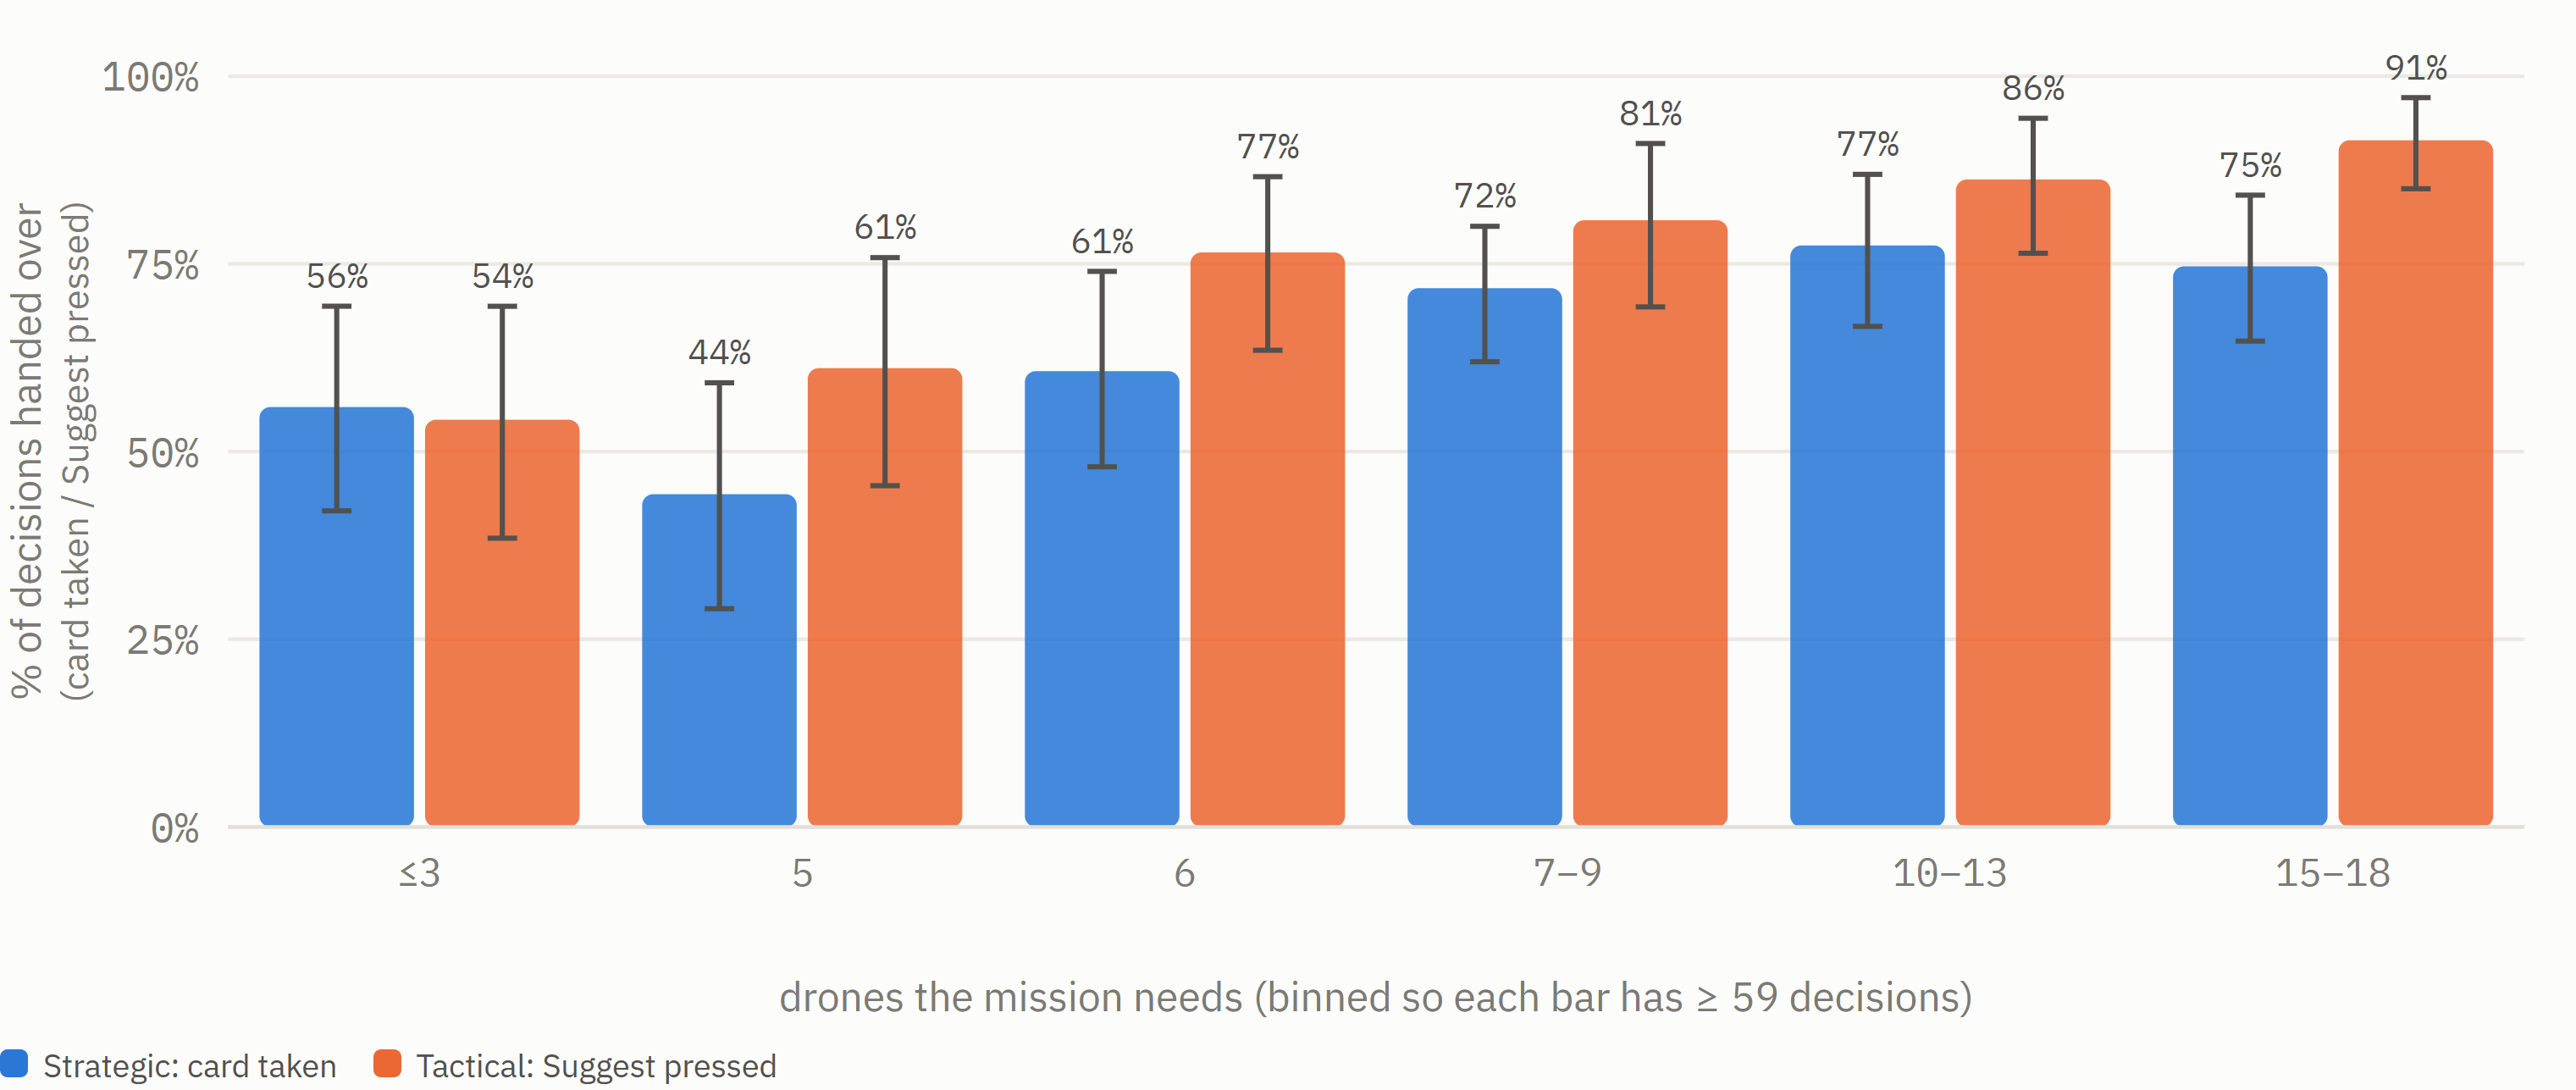
\includegraphics[width=\linewidth,height=0.55\textheight,keepaspectratio]{figs/results/f-size-decides__both__main.png}
\caption{\textbf{Both tiers on one axis: the bigger the mission, the more it is handed over}}
\label{fig:res:size-decides:both}
\end{figure}

\paragraph*{Key numbers.}

\begin{itemize}[leftmargin=1.2em,itemsep=1pt]

\item Strategic, per doubling of drones needed: odds $\times$1.62 [1.23, 2.15], p < .001 (606 decisions, 33 people)

\item Tactical, per doubling of drones needed: odds $\times$2.91 [2.03, 4.17], p < .001 (627 plans)

\item Both tiers, one shared slope: $\times$2.07 [1.64, 2.61], p < .001 (1,233 decisions); the tactical slope is steeper than the strategic one by $\times$1.38 [0.99, 1.91], p = .056 --- suggestive, not shown

\item Raw rates, smallest to largest bin: strategic 56\% $\rightarrow$ 75\%, tactical 54\% $\rightarrow$ 91\%

\item Arrival bursts (Strategic Heavy games, fixed per game): the seven 5-drone missions had on average 4.4 other missions arrive within 60 s of them, against 3.6 for the 3- and 6-drone one-type missions and 3.1 for every other mission; 6 of 7 arrived inside or straight after a burst; the seventh arrived 10 s into a game and got the card 69\% of the time

\end{itemize}

\paragraph*{Method.} {\small \textbf{Rows.} Strategic: all 606 strategy-card decisions (one per strategic choice). Tactical: all 627 non-recovery tactical plans whose mission size is known (630 minus 3 residual missions with no recorded need). \textbf{Size} = drones the mission needs: the sum of the primary requirements over its tasks --- the number an operator reads off the task badges, the same for both tiers. Binned so each bin has $\geq$ 59 decisions. \textbf{Intervals}: we resample whole people (2,000 times) and recompute the rate, so a person's decisions travel together and one heavy user cannot make an interval look tight. \textbf{Model}: a logistic GEE (a regression for yes/no outcomes that allows each person's decisions to be correlated) with size split into two parts --- this decision's size minus the person's own average size (the \emph{within-person} part) and the person's average (the between part); game and session are held fixed. The within-person odds ratio answers: ``when the same person meets a mission twice as big, how much do the odds that they hand it over change?'' Odds $\times$2 means, for example, a 60\% chance becomes 75\%. Both tiers in one model: the two tables stacked, one shared within-person slope plus a tier term; the tier $\times$ size term tests whether the slopes differ.}

\paragraph*{What participants said.} \regtext{10 of 33 state the size rule in debrief or interview (C03). The think-aloud adds at least six more who give the same reason while playing: P04, P06, P12, P20, P32 and P36. They do single-colour or few-drone missions themselves and hand over large, multi-colour, many-chain ones, usually because it is quicker. There is dissent. P30 thinks simple tasks are the ones the AI 'should be able to do even easier'. P29 switched direction mid-session ('if it's easy, then it's hard for it to do it wrong'). P20 kept complex orderings for themself, and P10 hands trivial one-option plans to Suggest.}

\paragraph*{Quotes selected for this section.}

\begin{quotelist}

\item ``I think if it's just one colour, I'm gonna do it, like, assign it myself, but if it's multiple colours, I think I'm gonna let, um, the AI choose for me, for the, the strategic side.''\,---\,P29 (think-aloud s2 0:17:33)

\item ``either it's a really big mission, and it's like, oh, I can trust it with a large mission. [\ldots{}] Or it's a simple mission, and I'll be like, oh, I can just bang it up myself.''\,---\,P11 (debrief 0:28:41)

\item ``I did feel like some of them I should do myself and I trusted it more with the complicated tasks''\,---\,P29 (debrief 0:24:54)

\item ``When they only needed a single colour of drone I tended to do it manually''\,---\,P34 (written interview)

\item ``I'll use the suggest, because there's a lot of drones here, so because there's a lot of drones to allocate''\,---\,P05 (think-aloud s1 0:09:36)

\end{quotelist}

\clearpage

\subsubsection{Person-adjusted: every size measure, both tiers, one picture}\label{sec:res:size-decides:models}

\noindent \passtag{for the paper}

\noindent \regtext{Each row is one within-person estimate: how the odds of handing over change when the same person meets a bigger job. Rows right of the line mean ``bigger $\rightarrow$ hand over more''. All size measures point the same way on both tiers; the two that do not clear the line are strategic tasks and the strategic slope once the cards are on screen. The bottom block holds the artefact checks. Dropping every illogical Conservative card leaves the effect in place. So does allowing for the fact that every operator played the same fixed missions, so one odd mission could otherwise make the interval look tight. With each mission as one point, the share handed over still rises with its size on both tiers.} (Figure~\ref{fig:res:size-decides:models})

\begin{figure}[H]
\centering
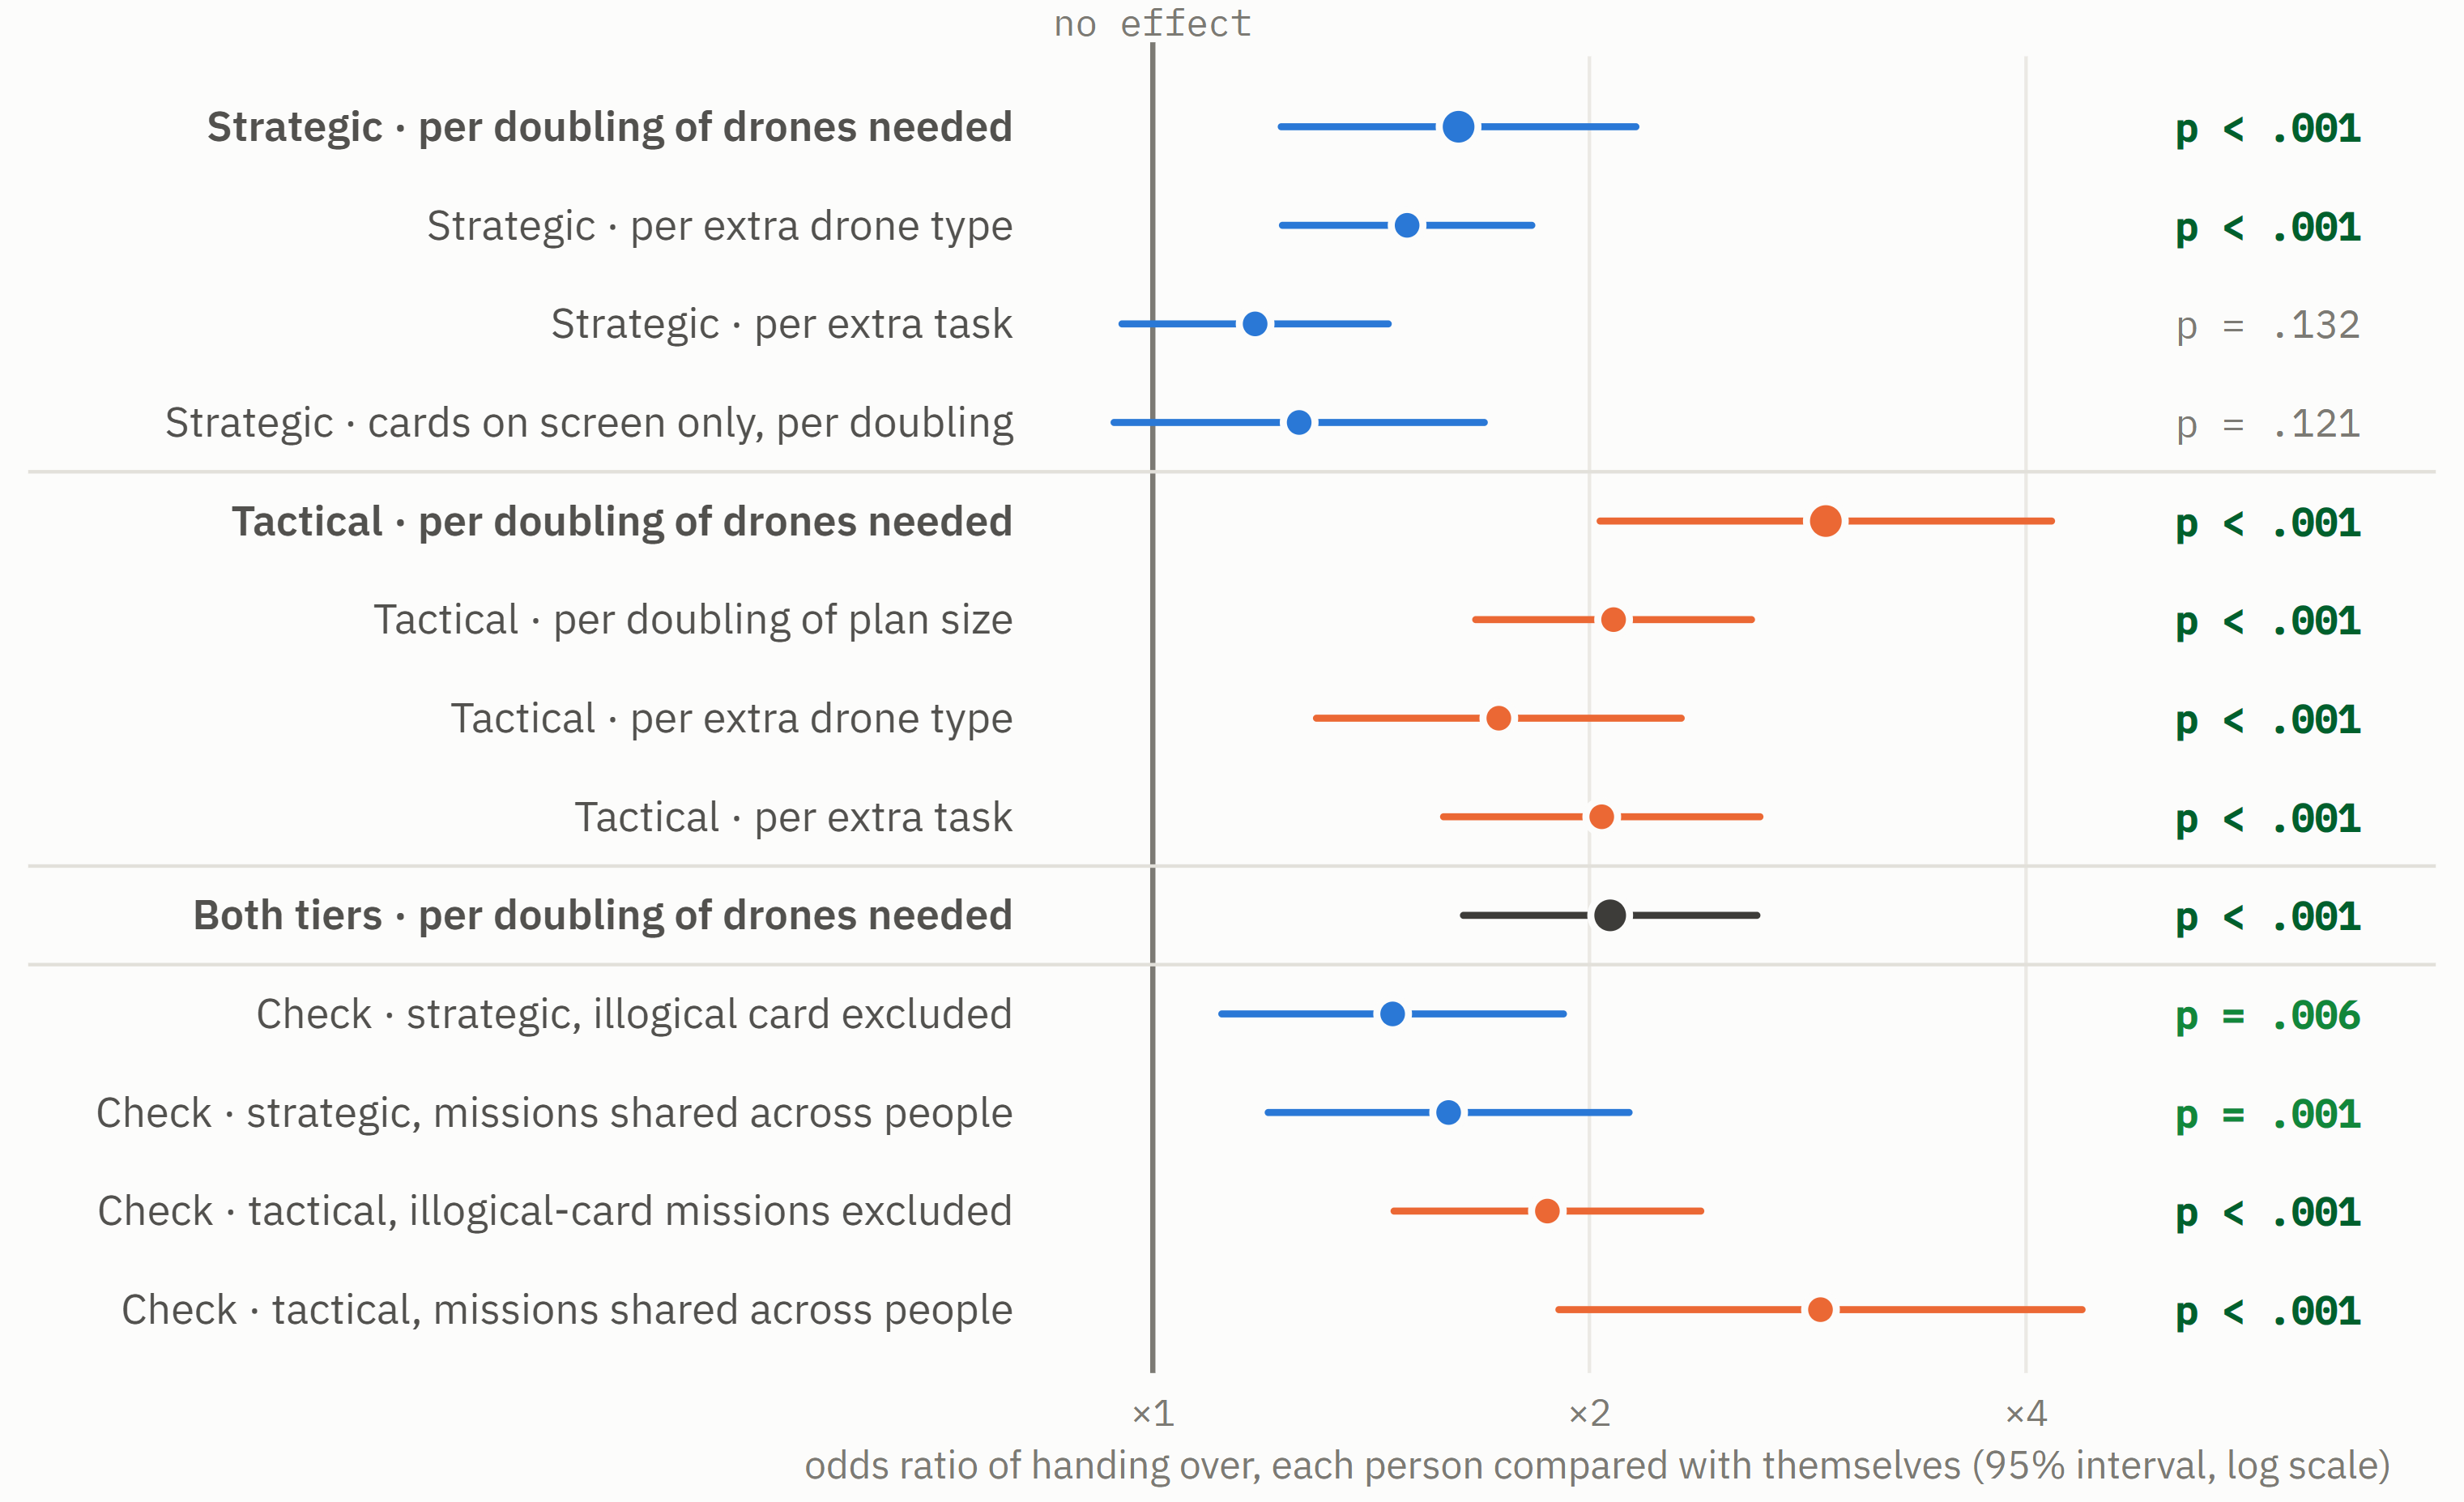
\includegraphics[width=\linewidth,height=0.55\textheight,keepaspectratio]{figs/results/f-size-decides__models__main.png}
\caption{\textbf{Person-adjusted: every size measure, both tiers, one picture}}
\label{fig:res:size-decides:models}
\end{figure}

\paragraph*{Key numbers.}

\begin{itemize}[leftmargin=1.2em,itemsep=1pt]

\item Strategic, illogical Conservative card excluded: $\times$1.46 [1.12, 1.92], p = .006 (474 decisions)

\item Missions shared across people (interval clustered on person and mission): strategic $\times$1.60 [1.20, 2.13], p = .001; tactical $\times$2.89 [1.91, 4.37], p < .001 (65 missions)

\item Each mission as one point (missions with $\geq$ 5 decisions): strategic $\rho$ = .63 over 41 missions, tactical $\rho$ = .69 over 41 (both p < .001)

\end{itemize}

\paragraph*{Method.} {\small GEE logistic models clustered on person (exchangeable correlation, small-sample ``bias-reduced'' standard errors), size split into within- and between-person parts, game and session held fixed. Odds ratio = how many times the odds of handing over multiply per unit of size. Read $\times$1.6 per doubling as: a person who takes the card on 60\% of 6-drone missions would be expected to take it on about 71\% of 12-drone ones.}

\paragraph*{What participants said.} \regtext{No one spoke to the model checks themselves. One check bears on what people said, though. Several said part of their hand-building on one-type missions was to avoid the Conservative card's spare drones of unneeded types (P19, P29, P21, P13). The finding's check that drops those illogical cards is the right control for that stated reason.}

\clearpage

\subsubsection{Tactical tier: Suggest rises with mission size, and goes with the strategic choice}\label{sec:res:size-decides:tactical}

\noindent \passtag{for the paper}

\noindent \regtext{In the tactical planner the dose-response is smooth whichever way size is measured: drones the mission needs, drones committed, tasks, drone types or plan size. The two bar colours split plans by how the mission was allocated strategically. A mission allocated from a strategy card gets Suggest more often than one allocated by hand, at every size and on every measure: \textbf{handing over at one tier goes with handing over at the other}. Comparing the same person's missions of the same size, a card-allocated mission gets Suggest at about twice the odds ($\times$2.10). The gap is wide on small missions (70\% vs 35\% at $\leq$3 drones) and small on the biggest (93\% vs 88\%), but that narrowing is both rates approaching 100\%; tested properly, the gap does not reliably shrink with size. Operators say this too: one participant (P10) described, while playing and again afterwards, that once they had taken the Aggressive card ``anything but Suggest'' made no sense, because a generous allocation leaves only one sensible way to assign the drones; two others (P05, P30) talked through taking a card and then pressing Suggest on the same mission. P10's reason, that it is the generous card that makes Suggest the obvious next step, does not show up across everyone: Suggest follows the Aggressive and the Conservative card at the same rate. The link is card vs hand, not which card. We use drones needed as the main measure: it is fixed by the mission, the same for every operator and what the task badges show. Plan size and team size also contain the operator's own strategic choice: for the same mission, a card commits about 11\% more drones than a hand allocation, so part of the strategic route is built into those x axes.} (Figure~\ref{fig:res:size-decides:tactical})

\begin{figure}[H]
\centering
\begin{subfigure}[t]{\linewidth}
\centering
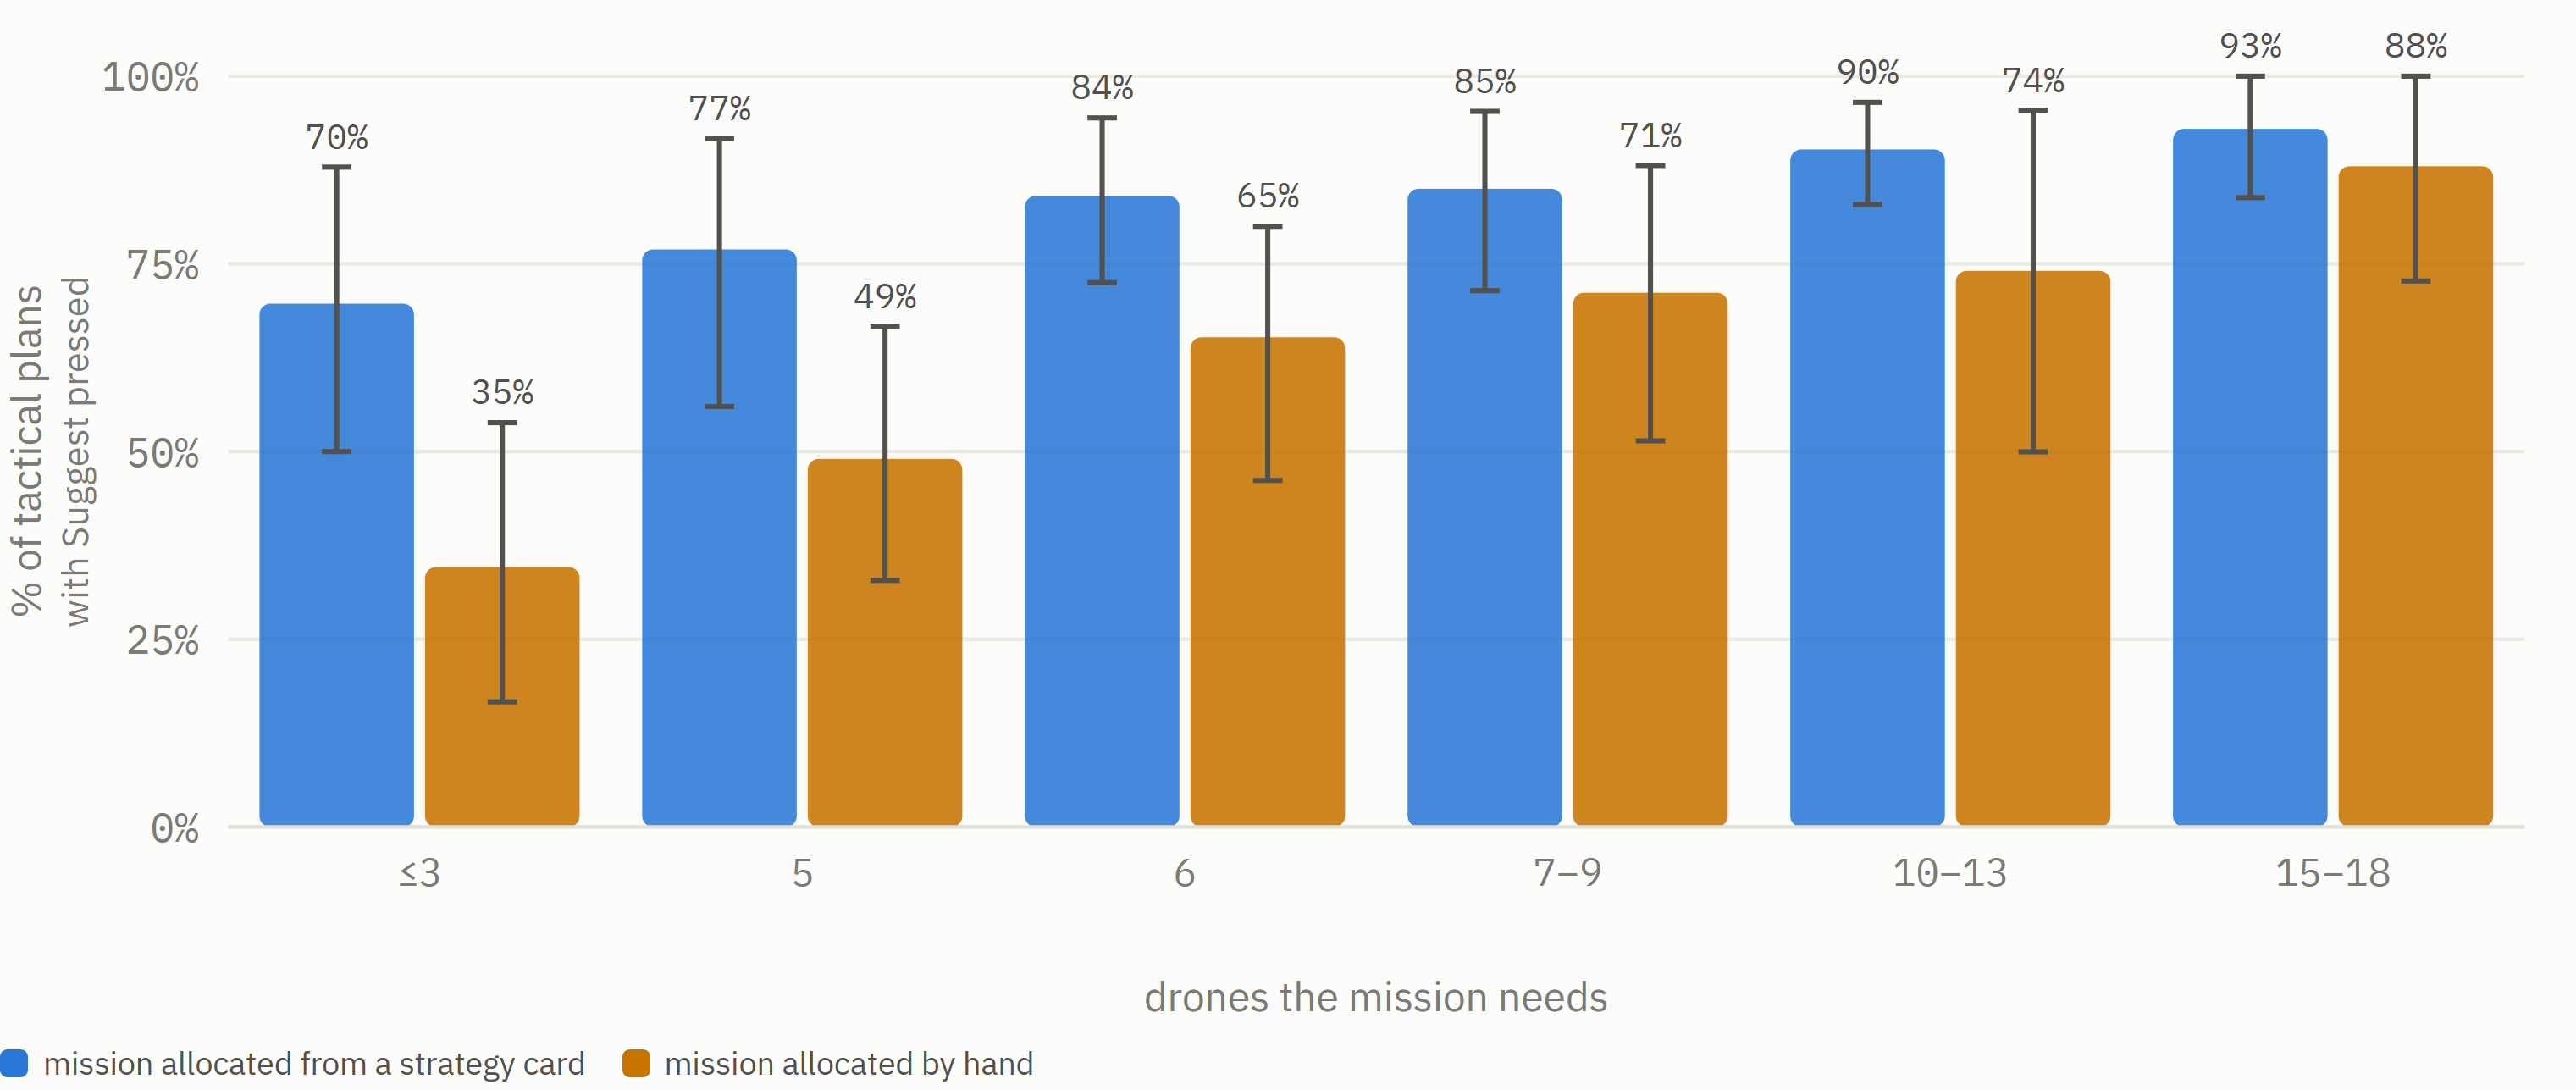
\includegraphics[width=\linewidth,height=0.23\textheight,keepaspectratio]{figs/results/f-size-decides__tactical__needed.png}
\caption{Size measured as drones needed.}
\label{fig:res:size-decides:tactical:needed}
\end{subfigure}
\par\smallskip
\begin{subfigure}[t]{\linewidth}
\centering
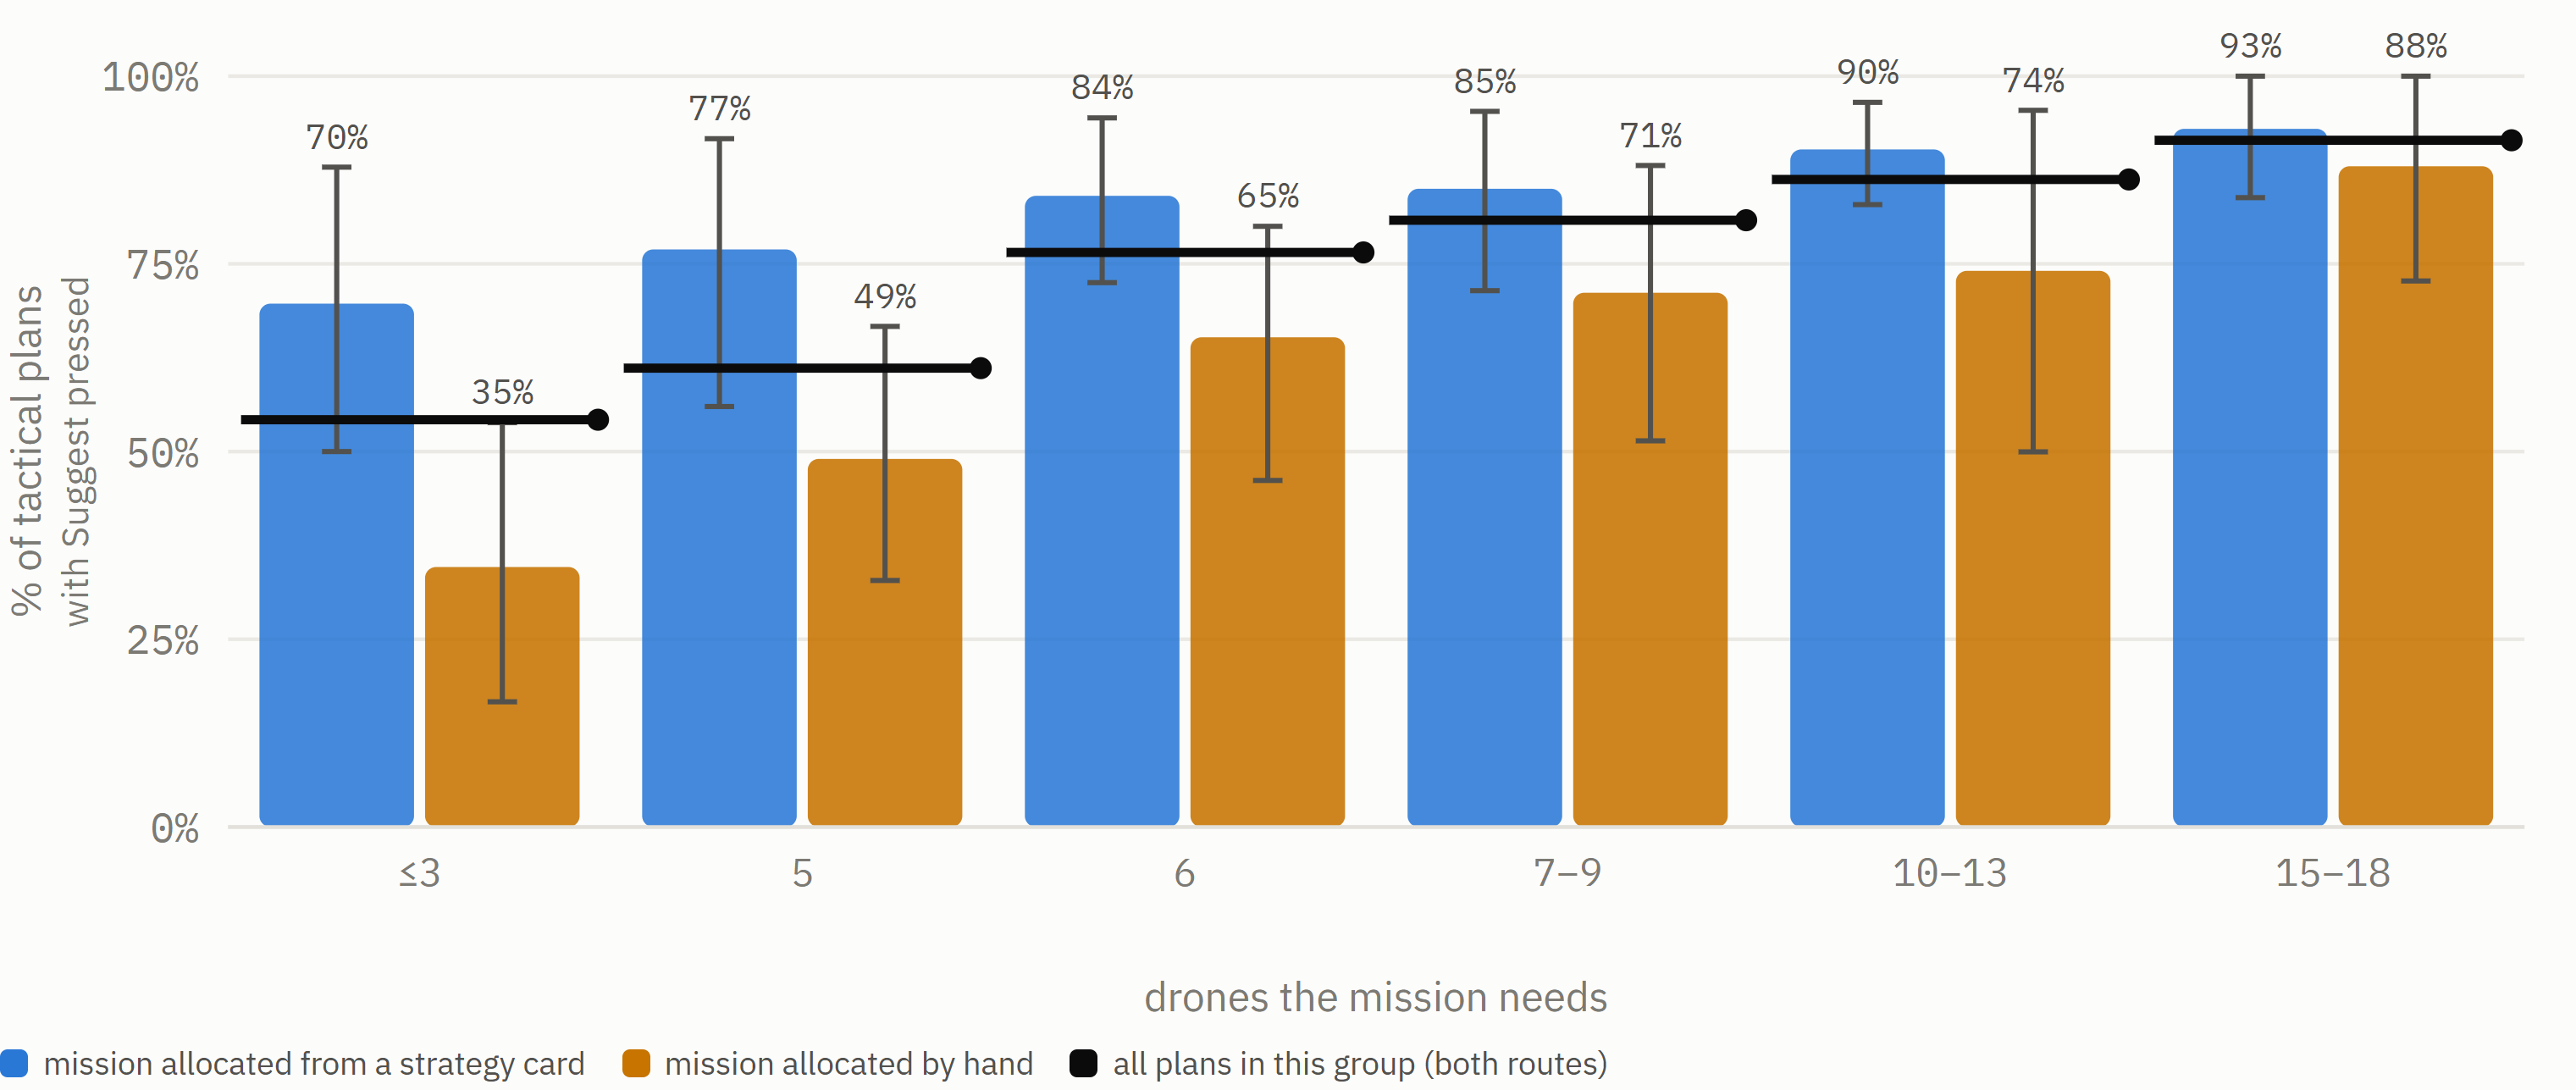
\includegraphics[width=\linewidth,height=0.23\textheight,keepaspectratio]{figs/results/f-size-decides__tactical__marker.png}
\caption{With a marker on each pair at the rate for all plans in that size group.}
\label{fig:res:size-decides:tactical:marker}
\end{subfigure}
\par\smallskip
\caption{\textbf{Tactical tier: Suggest rises with mission size, and goes with the strategic choice}}
\label{fig:res:size-decides:tactical}
\end{figure}

\paragraph*{Key numbers.}

\begin{itemize}[leftmargin=1.2em,itemsep=1pt]

\item Within person, per doubling of drones needed: odds $\times$2.91 [2.03, 4.17]; per extra task $\times$2.04 [1.59, 2.62]; per extra drone type $\times$1.73 [1.30, 2.31]; per doubling of drones committed $\times$2.51 [1.83, 3.45]; per doubling of plan size $\times$2.08 [1.67, 2.59] (all p < .001)

\item Allocated from a card vs by hand, same person, size held: $\times$2.10 [1.30, 3.40], p = .003 (drones needed); $\times$1.78 to $\times$2.12 on the other four measures, all p < .05

\item Aggressive card vs Conservative card, same person, drones needed held: $\times$0.88 [0.45, 1.75], p = .72 (400 plans); raw Suggest rate after Aggressive 81\% (200), after Conservative 89\% (203), after a hand allocation 63\% (227)

\item Does the gap shrink with size? Route $\times$ size: $\times$0.76 [0.30, 1.92], p = .56 (drones needed); p = .28 to .98 on the other measures: no reliable narrowing

\item Suggest pressed, card-allocated vs hand-allocated: $\leq$3 drones 70\% vs 35\%; 7--9 drones 85\% vs 71\%; 15--18 drones 93\% vs 88\%

\item Same mission, card vs hand: $\times$1.11 more drones committed and $\times$1.12 larger plan (both p < .001); drones needed, tasks and types identical by construction

\item Person level: people who take more cards also press Suggest more (Spearman $\rho$ = .37, p = .033, 33 people)

\item P10 in the log: Suggest on 8 of 9 Aggressive-allocated missions (never took the Conservative card) vs 6 of 9 hand-allocated

\end{itemize}

\paragraph*{Method.} {\small \textbf{Rows}: the 630 non-recovery tactical plans that were confirmed (the planner starts empty, so pressing Suggest is a deliberate choice); 627 have a known mission size. \textbf{Measures}: drones needed (sum of the task badges' requirements), drones committed (the team the strategic choice sent), tasks (residual missions left out), drone types, plan size (team $\times$ tasks). \textbf{Size model}: logistic GEE clustered on person, size split into this plan's size minus the person's own average (within) and that average (between), game and session fixed. \textbf{Route}: the same model plus ``allocated from a card'' (also split within/between person), so its odds ratio compares the same person's card-allocated and hand-allocated missions of the same size. \textbf{Narrowing test}: a route $\times$ size term (ratio of odds ratios; below 1 = the gap narrows as size grows). \textbf{Same-mission check}: regression of each measure on route with one dummy per mission, so only operators who met the same mission are compared.}

\paragraph*{What participants said.} \regtext{Three people tie the two tiers together the way the logs do (card-allocated missions get Suggest more). P10 says repeatedly that once they have taken the Aggressive card there is 'only really one way' to assign, so Suggest is the obvious next step. P05 and P30 take a card and then press Suggest on the same mission. The same continuity runs the other way for P21, who lays out a plan in their head while building the allocation by hand and says it would 'disrupt my thought process' to switch to Suggest for the tactical step; P30 likewise finds it easier to give the assistant resources and let it optimise. The opposite pairing is said too. P18 takes a card and then plans a routine mission by hand, and P26 and P28 build strategic allocations by hand but press Suggest. On size, the reasons given are drag-and-drop effort and the number of combinations or chains.}

\paragraph*{Quotes selected for this section.}

\begin{quotelist}

\item ``Now I'm using the suggestion because I took the aggressive approach which means I know that I have enough drones.''\,---\,P10 (think-aloud s2 0:13:08)

\item ``Better to use tac agent when using the aggressive strat agent''\,---\,P10 (written interview) (paraphrase)

\item ``If I look at a mission with 15 drones and I need to move two or three chains, that's just going to take me about a minute, and it's just no point.''\,---\,P11 (debrief 0:29:41)

\item ``Dragging 14 drones is going to take way more time than hitting the assign and waiting for eight seconds.''\,---\,P10 (think-aloud s2 0:13:43)

\end{quotelist}

\clearpage

\subsubsection{Card then Suggest, person by person: a broad tilt, but a few people carry much of it}\label{sec:res:size-decides:route-people}

\noindent \passtag{numbers only}

\noindent \regtext{Is the card $\rightarrow$ Suggest link down to a few people? Partly. Each bar is one person: how much more often they pressed Suggest on missions they had allocated from a card than on ones they allocated by hand, with mission size held (the second view shows the two raw rates). Of the 26 people who did both often enough to compare, \textbf{17 lean towards Suggest after a card, 8 the other way, 1 neither}, so it is not one or two people. But it is uneven: the three biggest gaps (P13, P06, P15) make up about half of the total, and the person-adjusted odds ratio ($\times$2.10 for everyone) falls to $\times$1.63 without those three (still p = .03) and to $\times$1.46 without the top five (p = .08). Leaving out any single person never moves it outside $\times$1.90--$\times$2.40. So: a general tendency, strongest in a handful of people. Seven people cannot show a gap at all, six because they nearly always took a card before planning.} (Figure~\ref{fig:res:size-decides:route-people})

\begin{figure}[H]
\centering
\begin{subfigure}[t]{\linewidth}
\centering
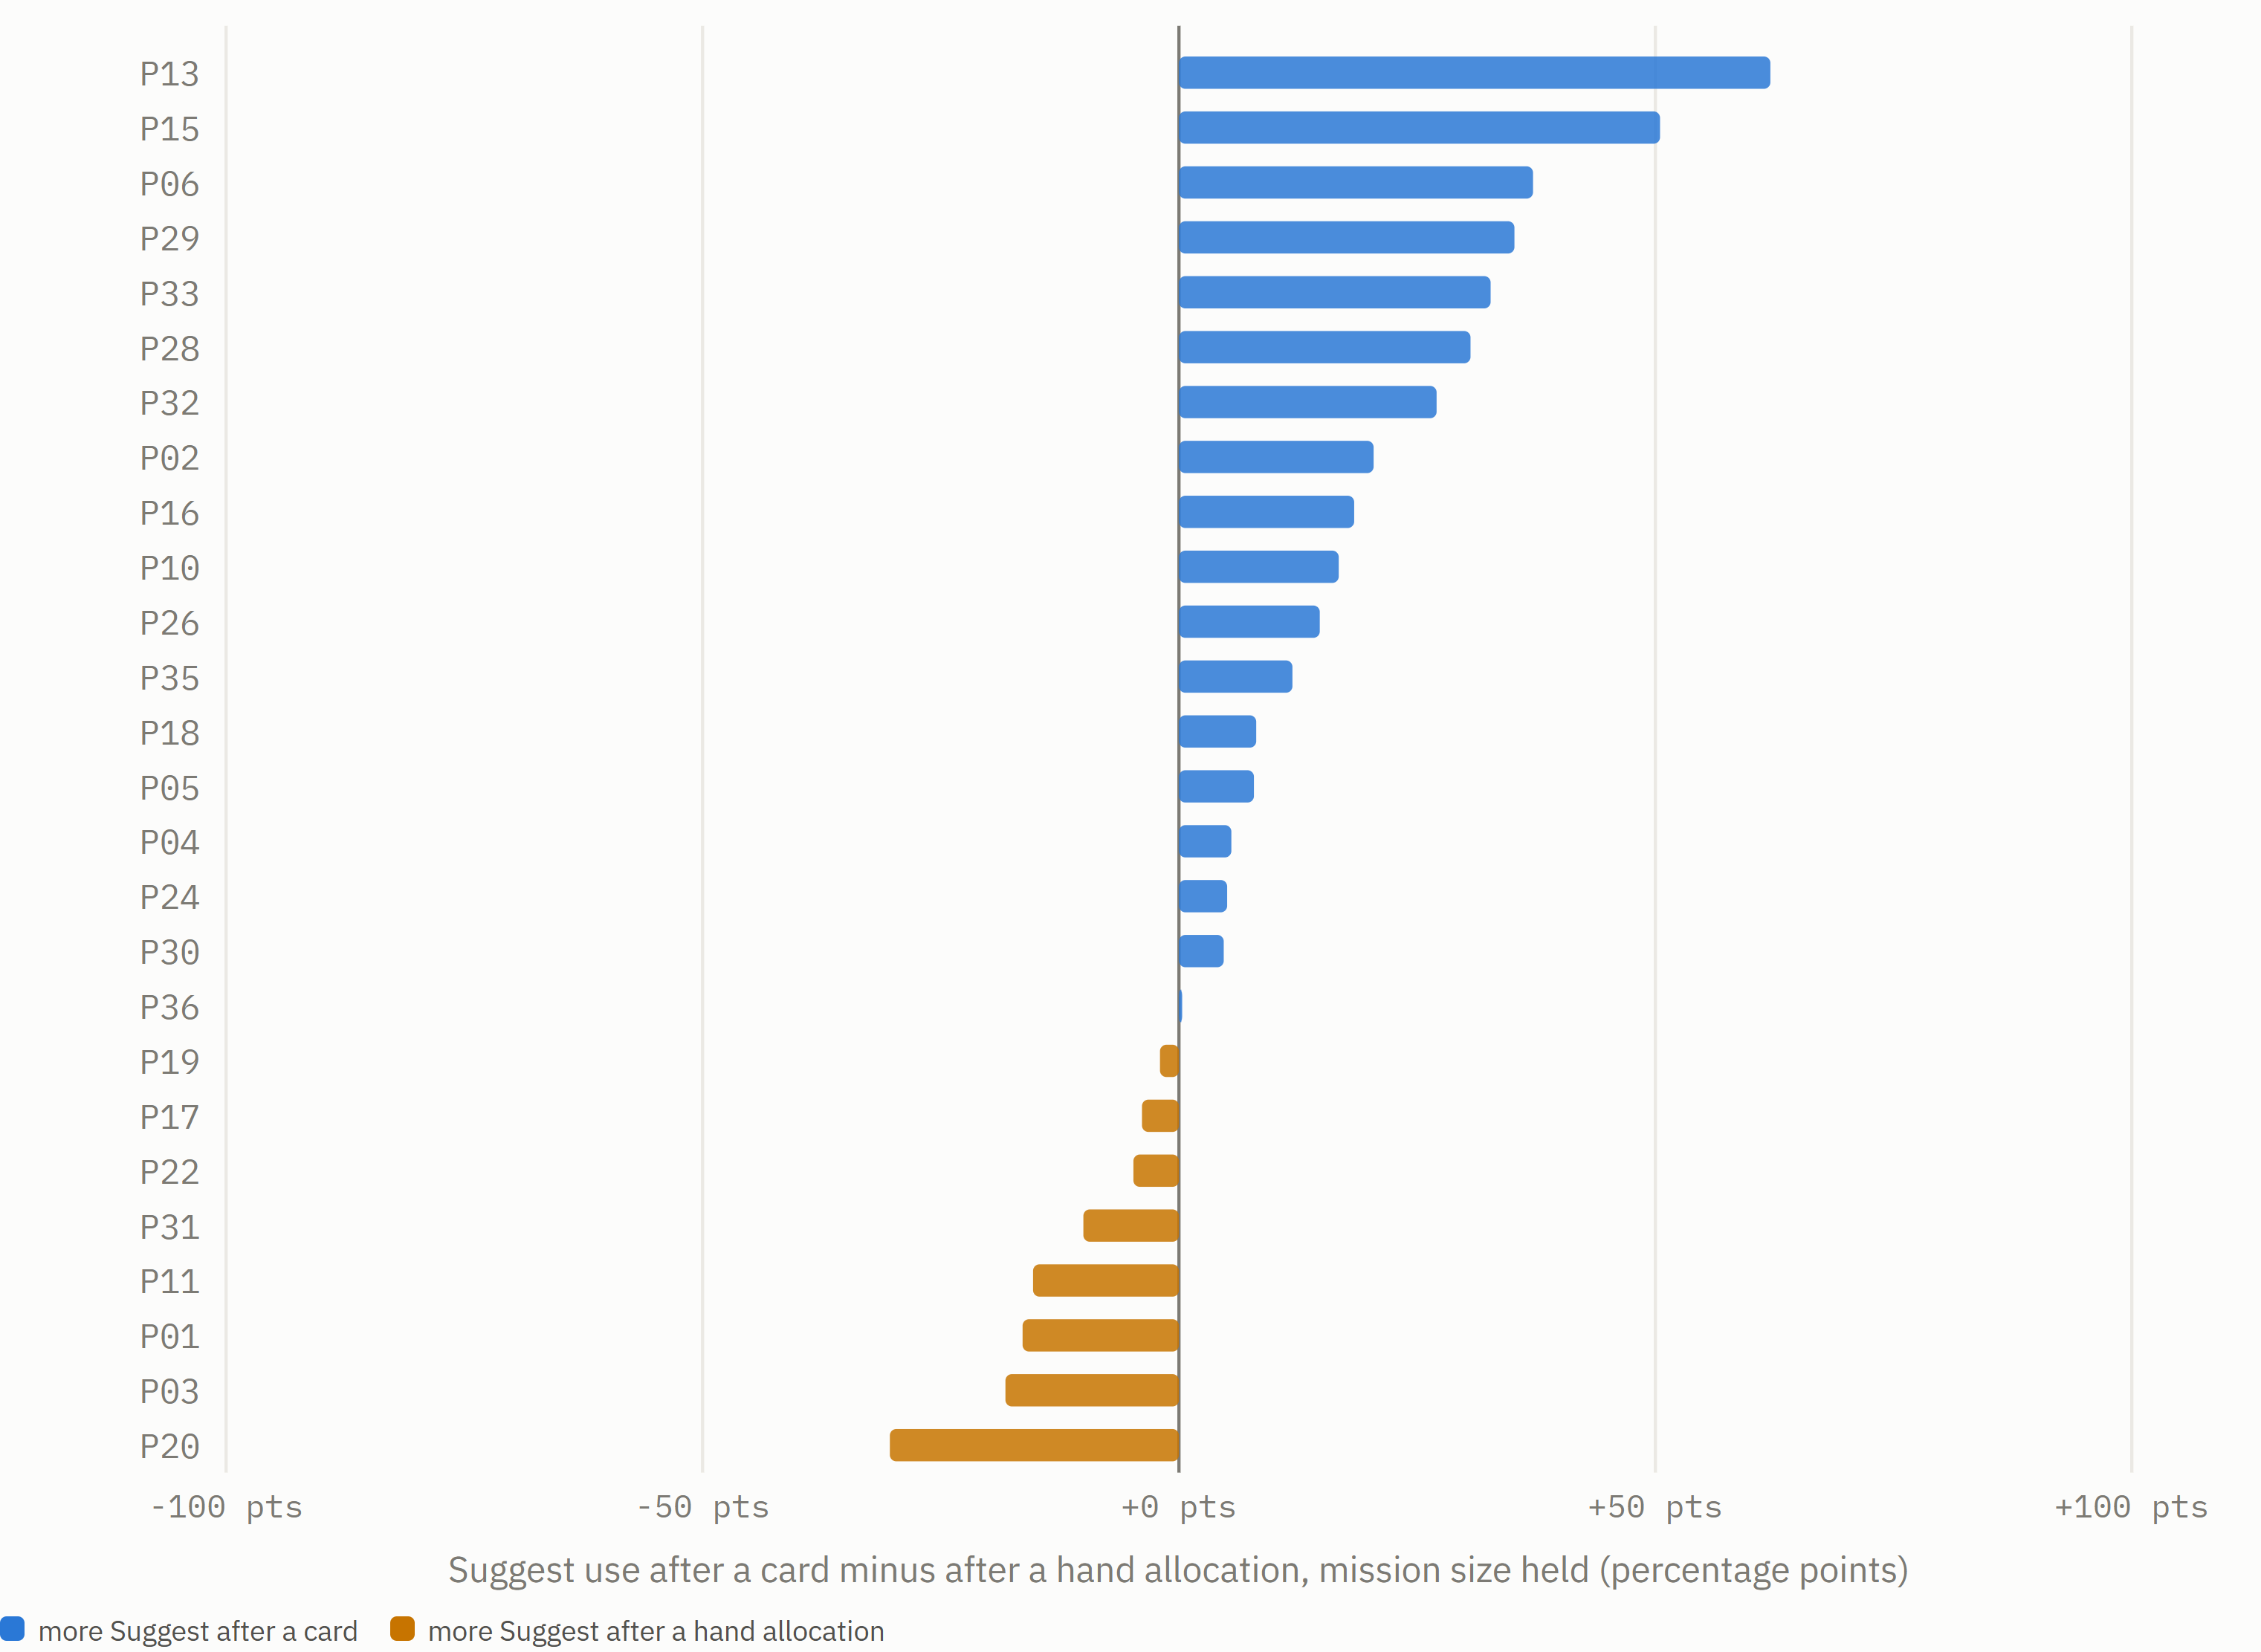
\includegraphics[width=\linewidth,height=0.23\textheight,keepaspectratio]{figs/results/f-size-decides__route-people__gap.png}
\caption{Each person's gap, mission size held.}
\label{fig:res:size-decides:route-people:gap}
\end{subfigure}
\par\smallskip
\begin{subfigure}[t]{\linewidth}
\centering
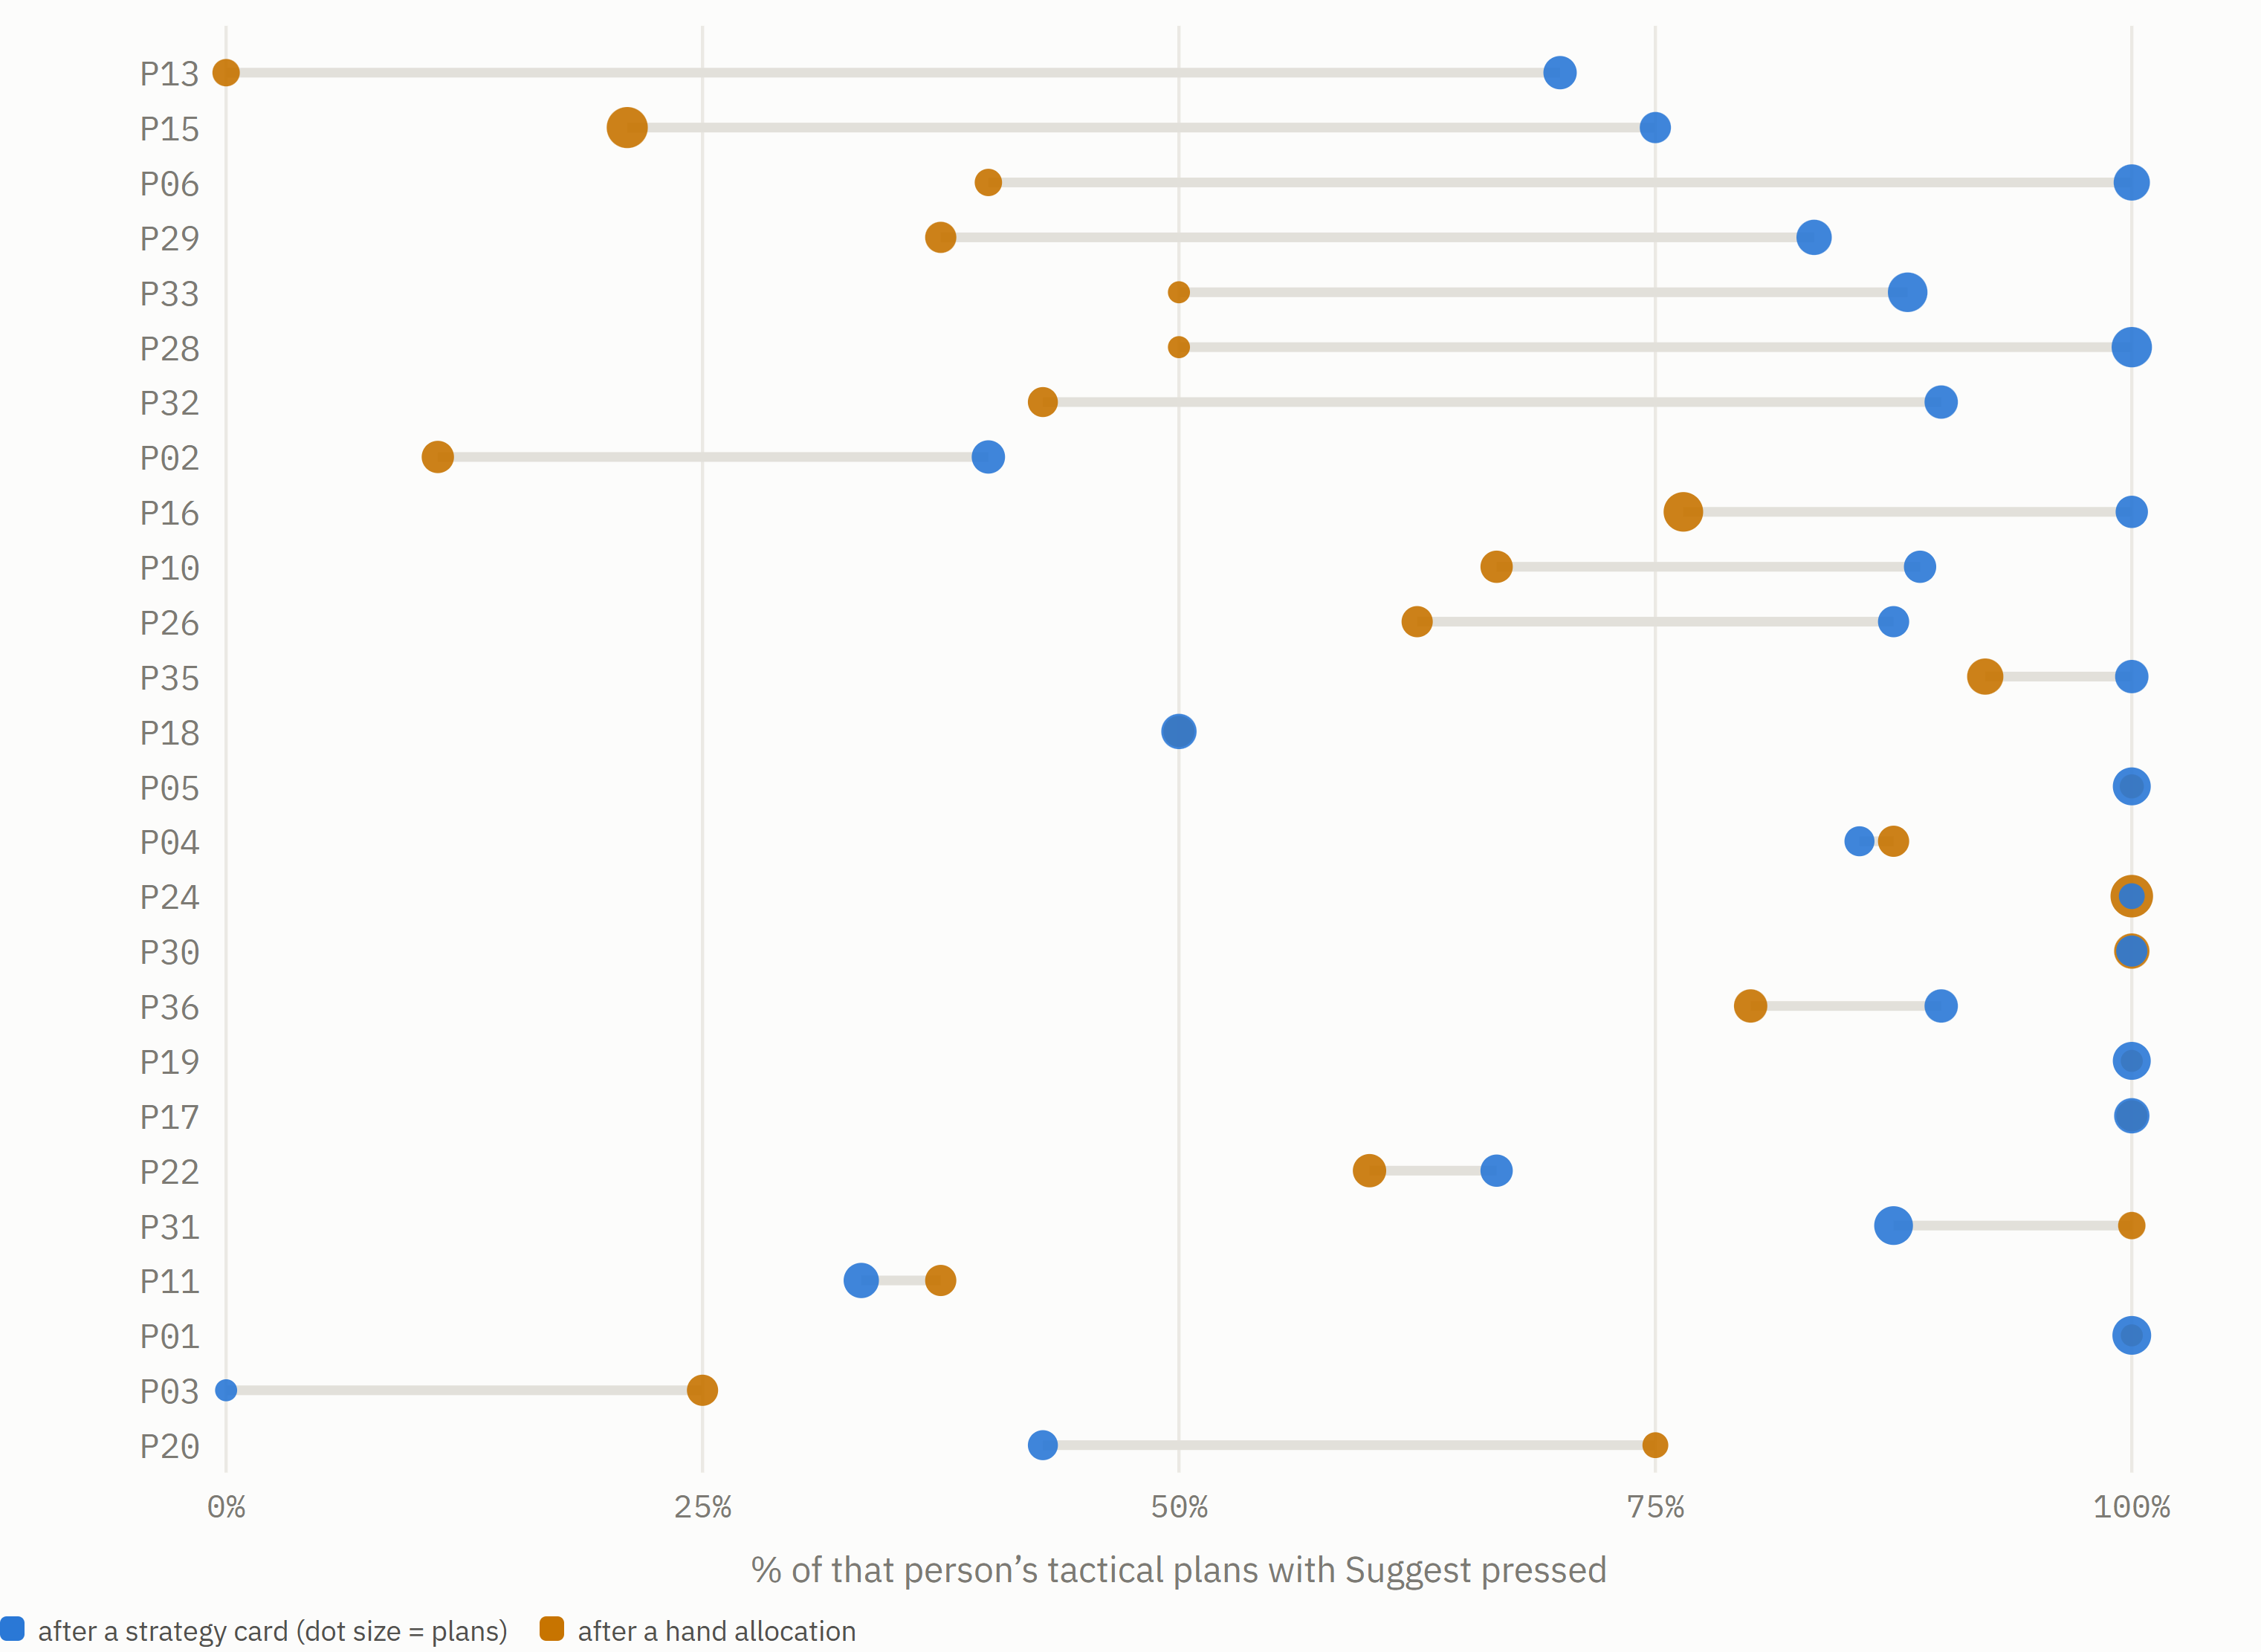
\includegraphics[width=\linewidth,height=0.23\textheight,keepaspectratio]{figs/results/f-size-decides__route-people__rates.png}
\caption{Each person's two raw rates.}
\label{fig:res:size-decides:route-people:rates}
\end{subfigure}
\par\smallskip
\caption{\textbf{Card then Suggest, person by person: a broad tilt, but a few people carry much of it}}
\label{fig:res:size-decides:route-people}
\end{figure}

\paragraph*{Key numbers.}

\begin{itemize}[leftmargin=1.2em,itemsep=1pt]

\item People with $\geq$ 2 plans each way: 26. Gap (size held) positive 17, negative 8, none 1; sign test p = .11; mean gap +11 points.

\item Card vs hand odds ratio, everyone $\times$2.10; leaving out any one person $\times$1.90 (without P15) to $\times$2.40 (without P11), always p < .05.

\item Without the largest gaps: top 1 (P13) $\times$1.97, p = .006; top 3 (P06, P13, P15) $\times$1.63 [1.05, 2.52], p = .03; top 5 $\times$1.46 [0.96, 2.22], p = .08; top 8 $\times$1.23, p = .34.

\item The three largest gaps are 52\% of the summed gap. Not comparable: 6 people almost only planned after a card, 1 almost only after a hand allocation.

\item Also holding fixed whether the mission needs one drone type: $\times$2.13 [1.30, 3.49]; and the number of tasks too: $\times$2.06 [1.24, 3.43], p = .005.

\end{itemize}

\paragraph*{Method.} {\small Rows: the 627 tactical plans with a known mission size, split by how the mission was allocated (strategy card or by hand). For each person with at least two plans each way, the gap is the mean of (pressed Suggest $-$ expected) after a card minus the same after a hand allocation, where 'expected' comes from a person-clustered model of Suggest on mission size (drones needed, within and between person), game and session, without the route; so the gap compares missions of the same size. The odds ratio is the section above's route model (card vs hand, same person, size held), refitted leaving out one person at a time, and then leaving out the people with the 1, 3, 5 and 8 largest gaps. The sign test asks whether more people lean one way than chance.}

\paragraph*{What participants said.} \regtext{The people at the ends of the chart, in their own words. \textbf{Strongest tilt} (P13, P15, P06, then P29): none of them talks about linking the two steps. They describe a rule for the whole mission: P15 hands over when there are 'too many decisions', P29 does one-colour missions themself and lets the assistant take multi-colour ones, and P06 drags and drops less as the work piles up. P13's hand allocations are disagreements with over-stocked cards ('why would I spend more resources'), and they say 'I always let the agent do it first' on the tactical step, yet none of their five plans after a hand allocation used Suggest. Their words do not explain their gap. \textbf{Leaning the other way} (P20, P03, P11, P31): their hand allocations are of a different kind. P20 builds by hand when the card cannot be met ('I've run out of blues') and then presses Suggest because the mission has many tasks. P03 works every allocation out first and checks the card against it. P11 rarely presses Suggest at all and does not want 'to be reduced to pressing allocate, suggest, deploy'. P31 lets Suggest get 'the majority of the way' whatever happened at the strategic step. \textbf{Only one route}: P21, who almost always allocated by hand, gives the clearest account of carrying a plan from one step to the next ('it's going to disrupt my thought process'). The card-only people (P07, P12, P14, P25, P27, P34) mostly give speed and urgency as the reason; P14 used the assistants 'for almost every allocation'.}

\clearpage

\subsubsection{Why the rule makes sense: the card pays only on big strategic jobs; Suggest is not slower}\label{sec:res:size-decides:speed}

\noindent \passtag{extra: may make it in}

\noindent \regtext{Each decision's time split into the time before the operator's first action and the time after it, by mission size, as stacked bars. \textbf{First action} = the first click on that decision: highlighting a card or changing a manual count (strategic; taking a card always needs a highlight first), pressing Suggest or dragging a drone (tactical). Before it, the strategic panel has two parts: the cards still loading (a forced wait of about 4.7 s; deciding by hand early can cut it short) and \textbf{idle time} with the cards on screen. The ``Time counted'' toggle drops the idle time, or everything before the first click. Strategic: counting everything, a card is much quicker than a manual build on three-type missions ($-$27\%) and no quicker on one-type ones (+22\%, not reliable). Card-takers sit idle about as long as manual builders (7 s vs 9--11 s on average), so dropping idle time makes the card look better everywhere; on one-type missions it then ties with a manual build ($-$8\%), and on three-type missions the card is 44\% quicker. Deciding before the cards load (7 s) beats the card when everything is counted and is level with it once idle time is dropped, on one-type missions. Tactical, on all 627 plans: by hand and with Suggest take about the same planner time (29 vs 27 s on average), and the same with the idle time removed (15 vs 17 s); held to the same person and size the difference is under 1 s. On large missions hand-building takes longer (32 vs 22 s without idle time), but the size $\times$ Suggest term is not reliable. So the speed story is clear on the strategic tier, and on the tactical tier Suggest saves no planner time. Its time saving is in carrying out (next section).} (Figure~\ref{fig:res:size-decides:speed})

\begin{figure}[H]
\centering
\begin{subfigure}[t]{0.495\linewidth}
\centering
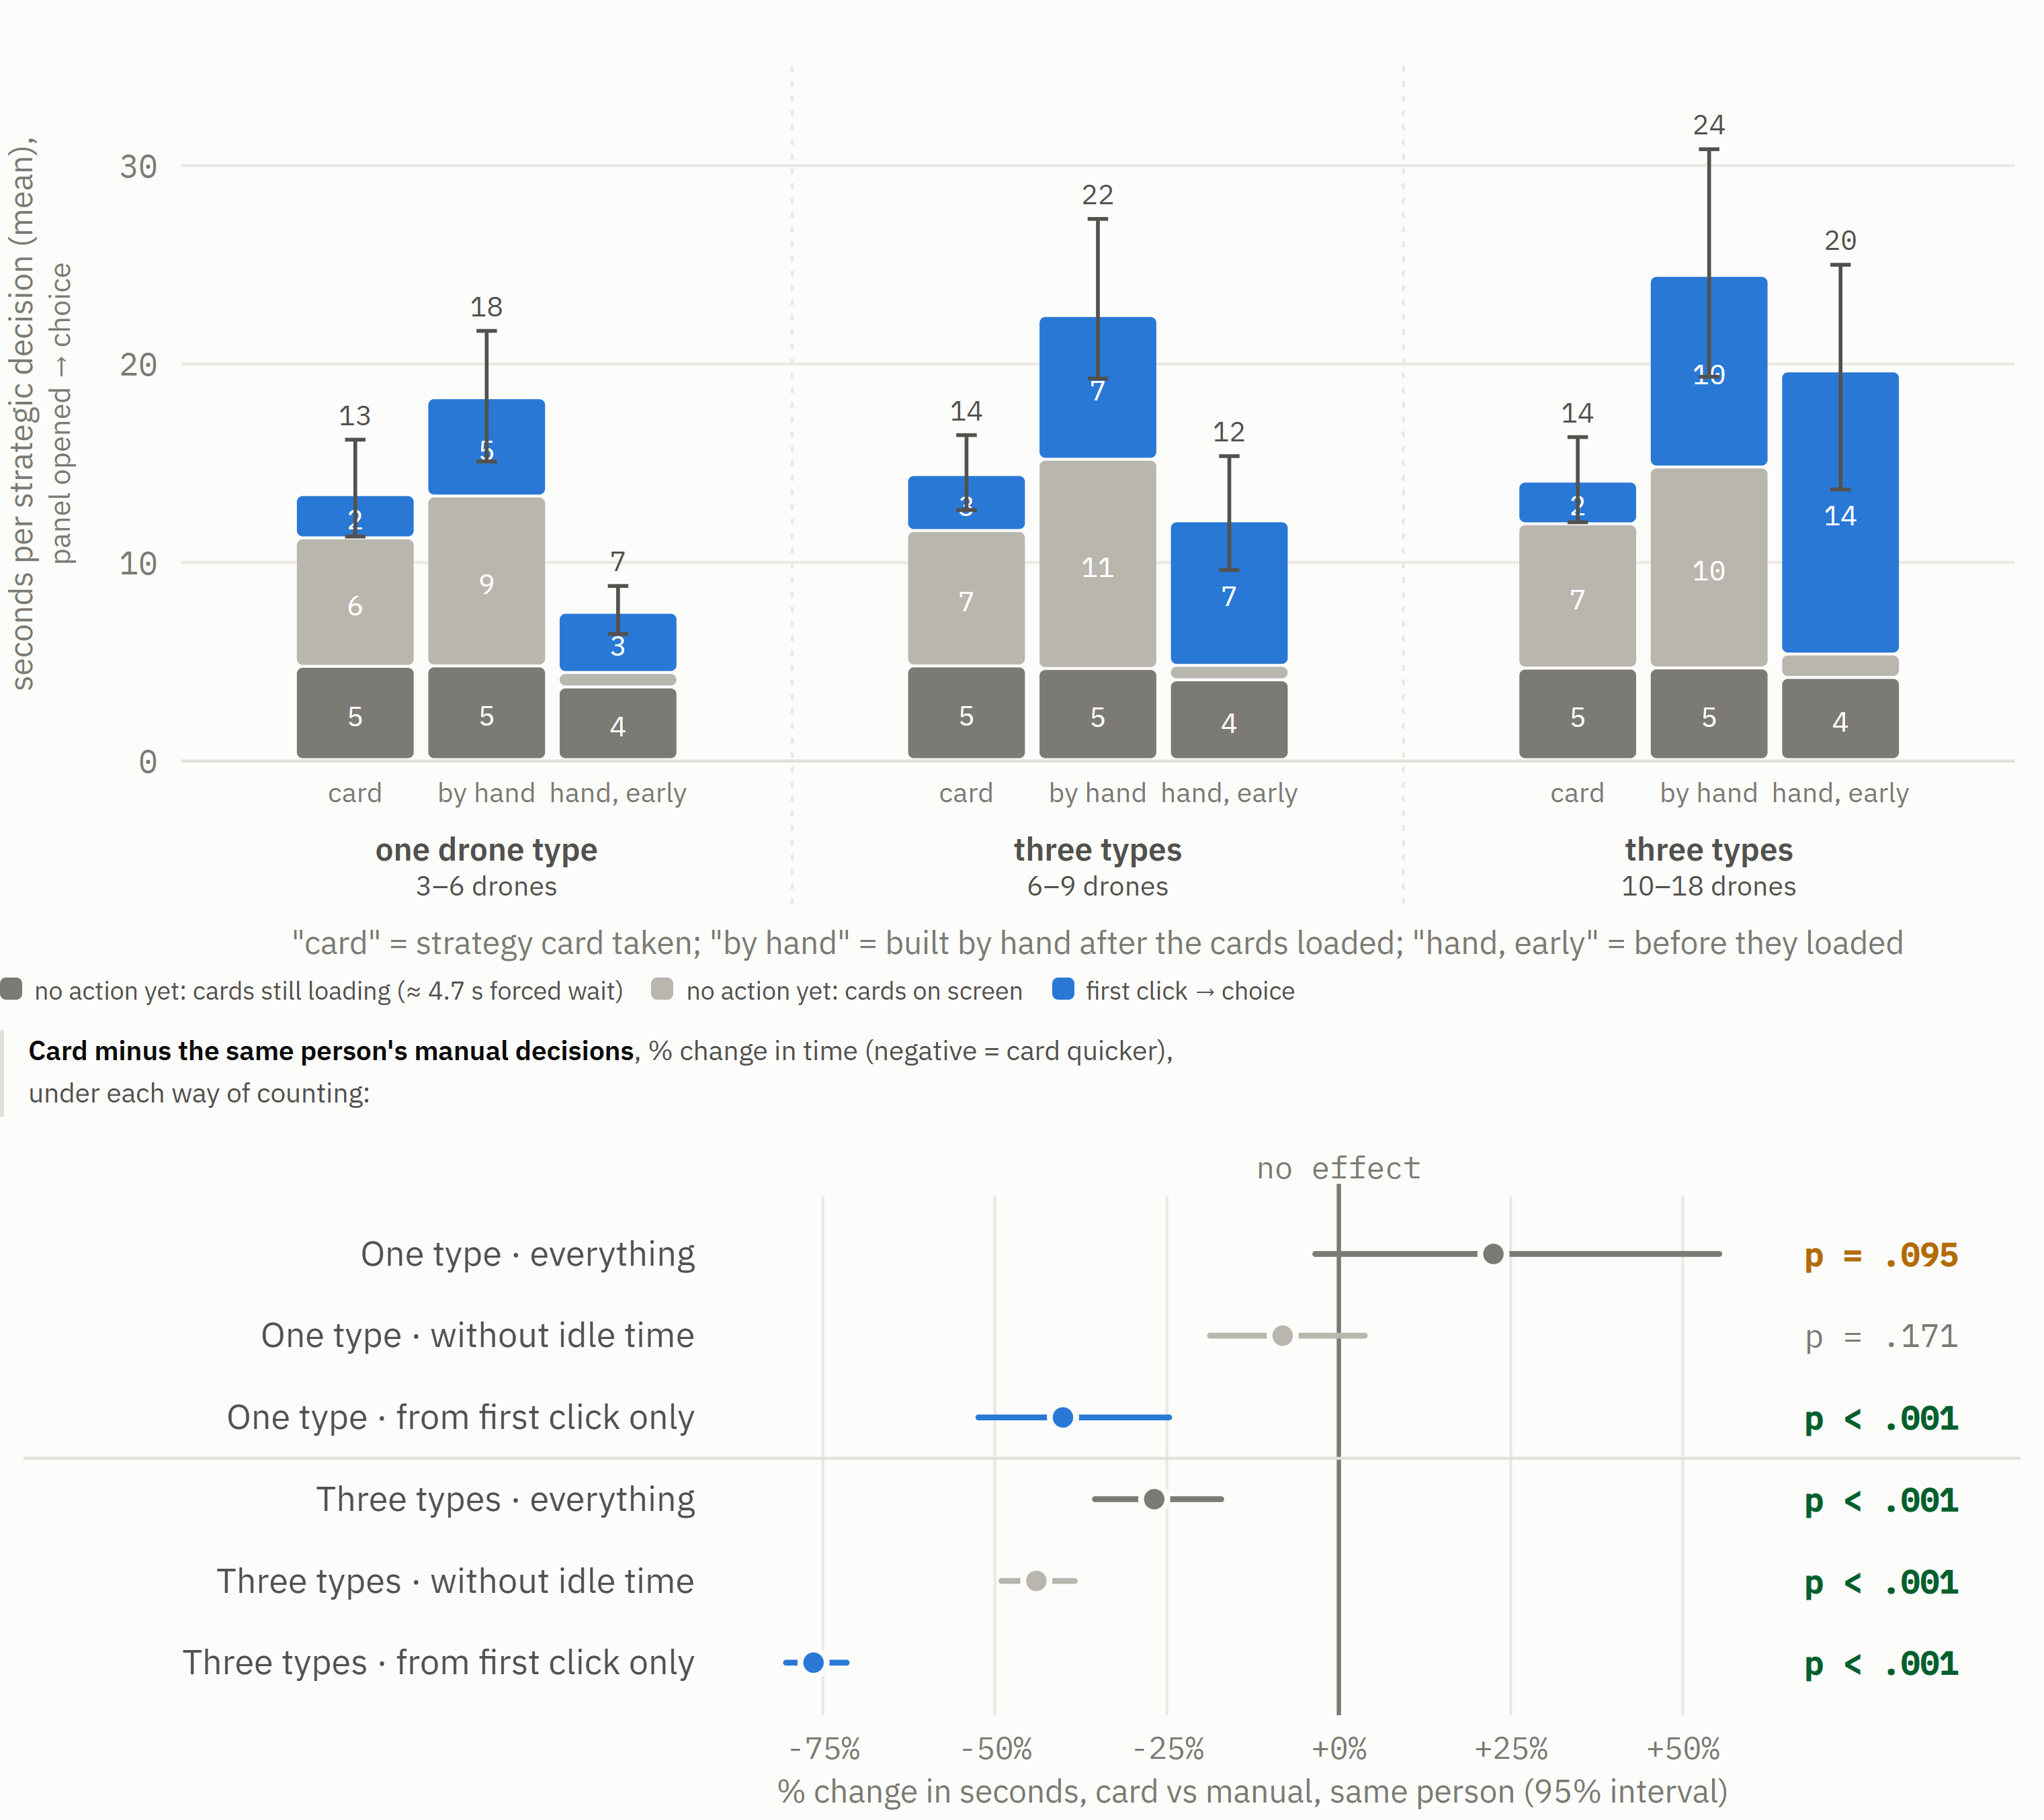
\includegraphics[width=\linewidth,height=0.23\textheight,keepaspectratio]{figs/results/f-size-decides__speed__strat-all.png}
\caption{Strategic tier, all time counted.}
\label{fig:res:size-decides:speed:strat-all}
\end{subfigure}
\hfill
\begin{subfigure}[t]{0.495\linewidth}
\centering
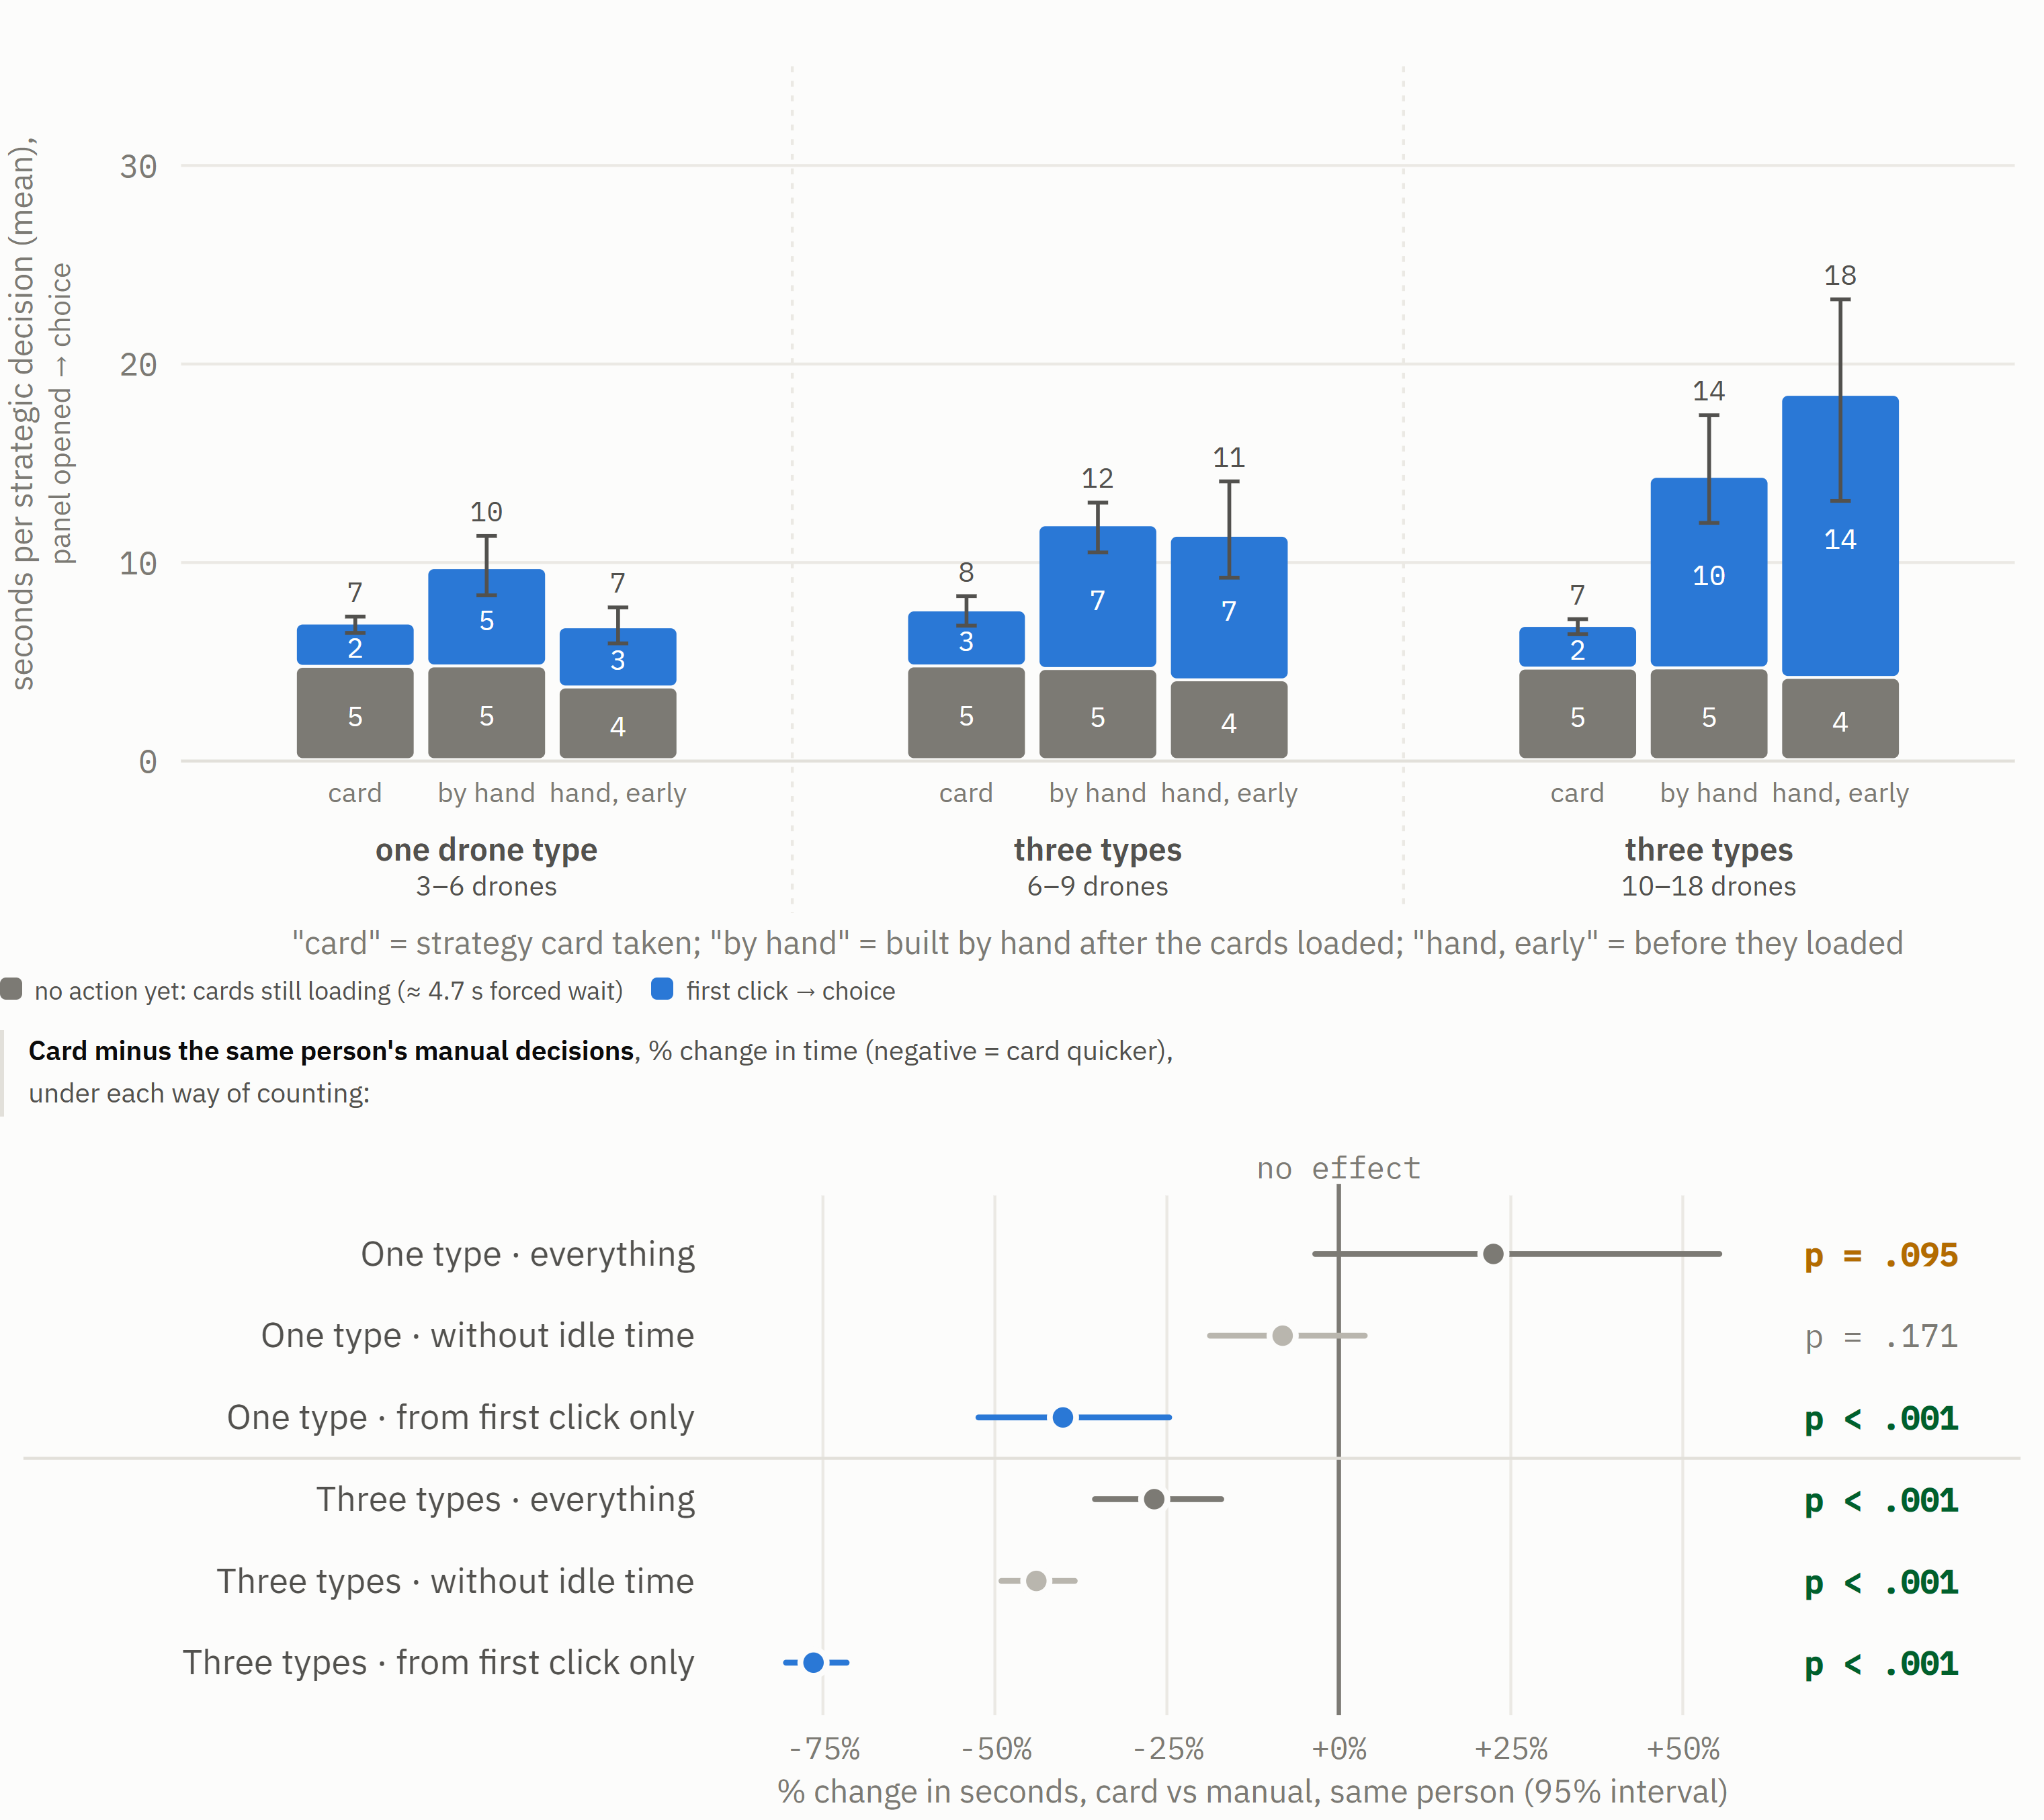
\includegraphics[width=\linewidth,height=0.23\textheight,keepaspectratio]{figs/results/f-size-decides__speed__strat-noidle.png}
\caption{Strategic tier, idle time removed.}
\label{fig:res:size-decides:speed:strat-noidle}
\end{subfigure}
\par\smallskip
\begin{subfigure}[t]{0.495\linewidth}
\centering
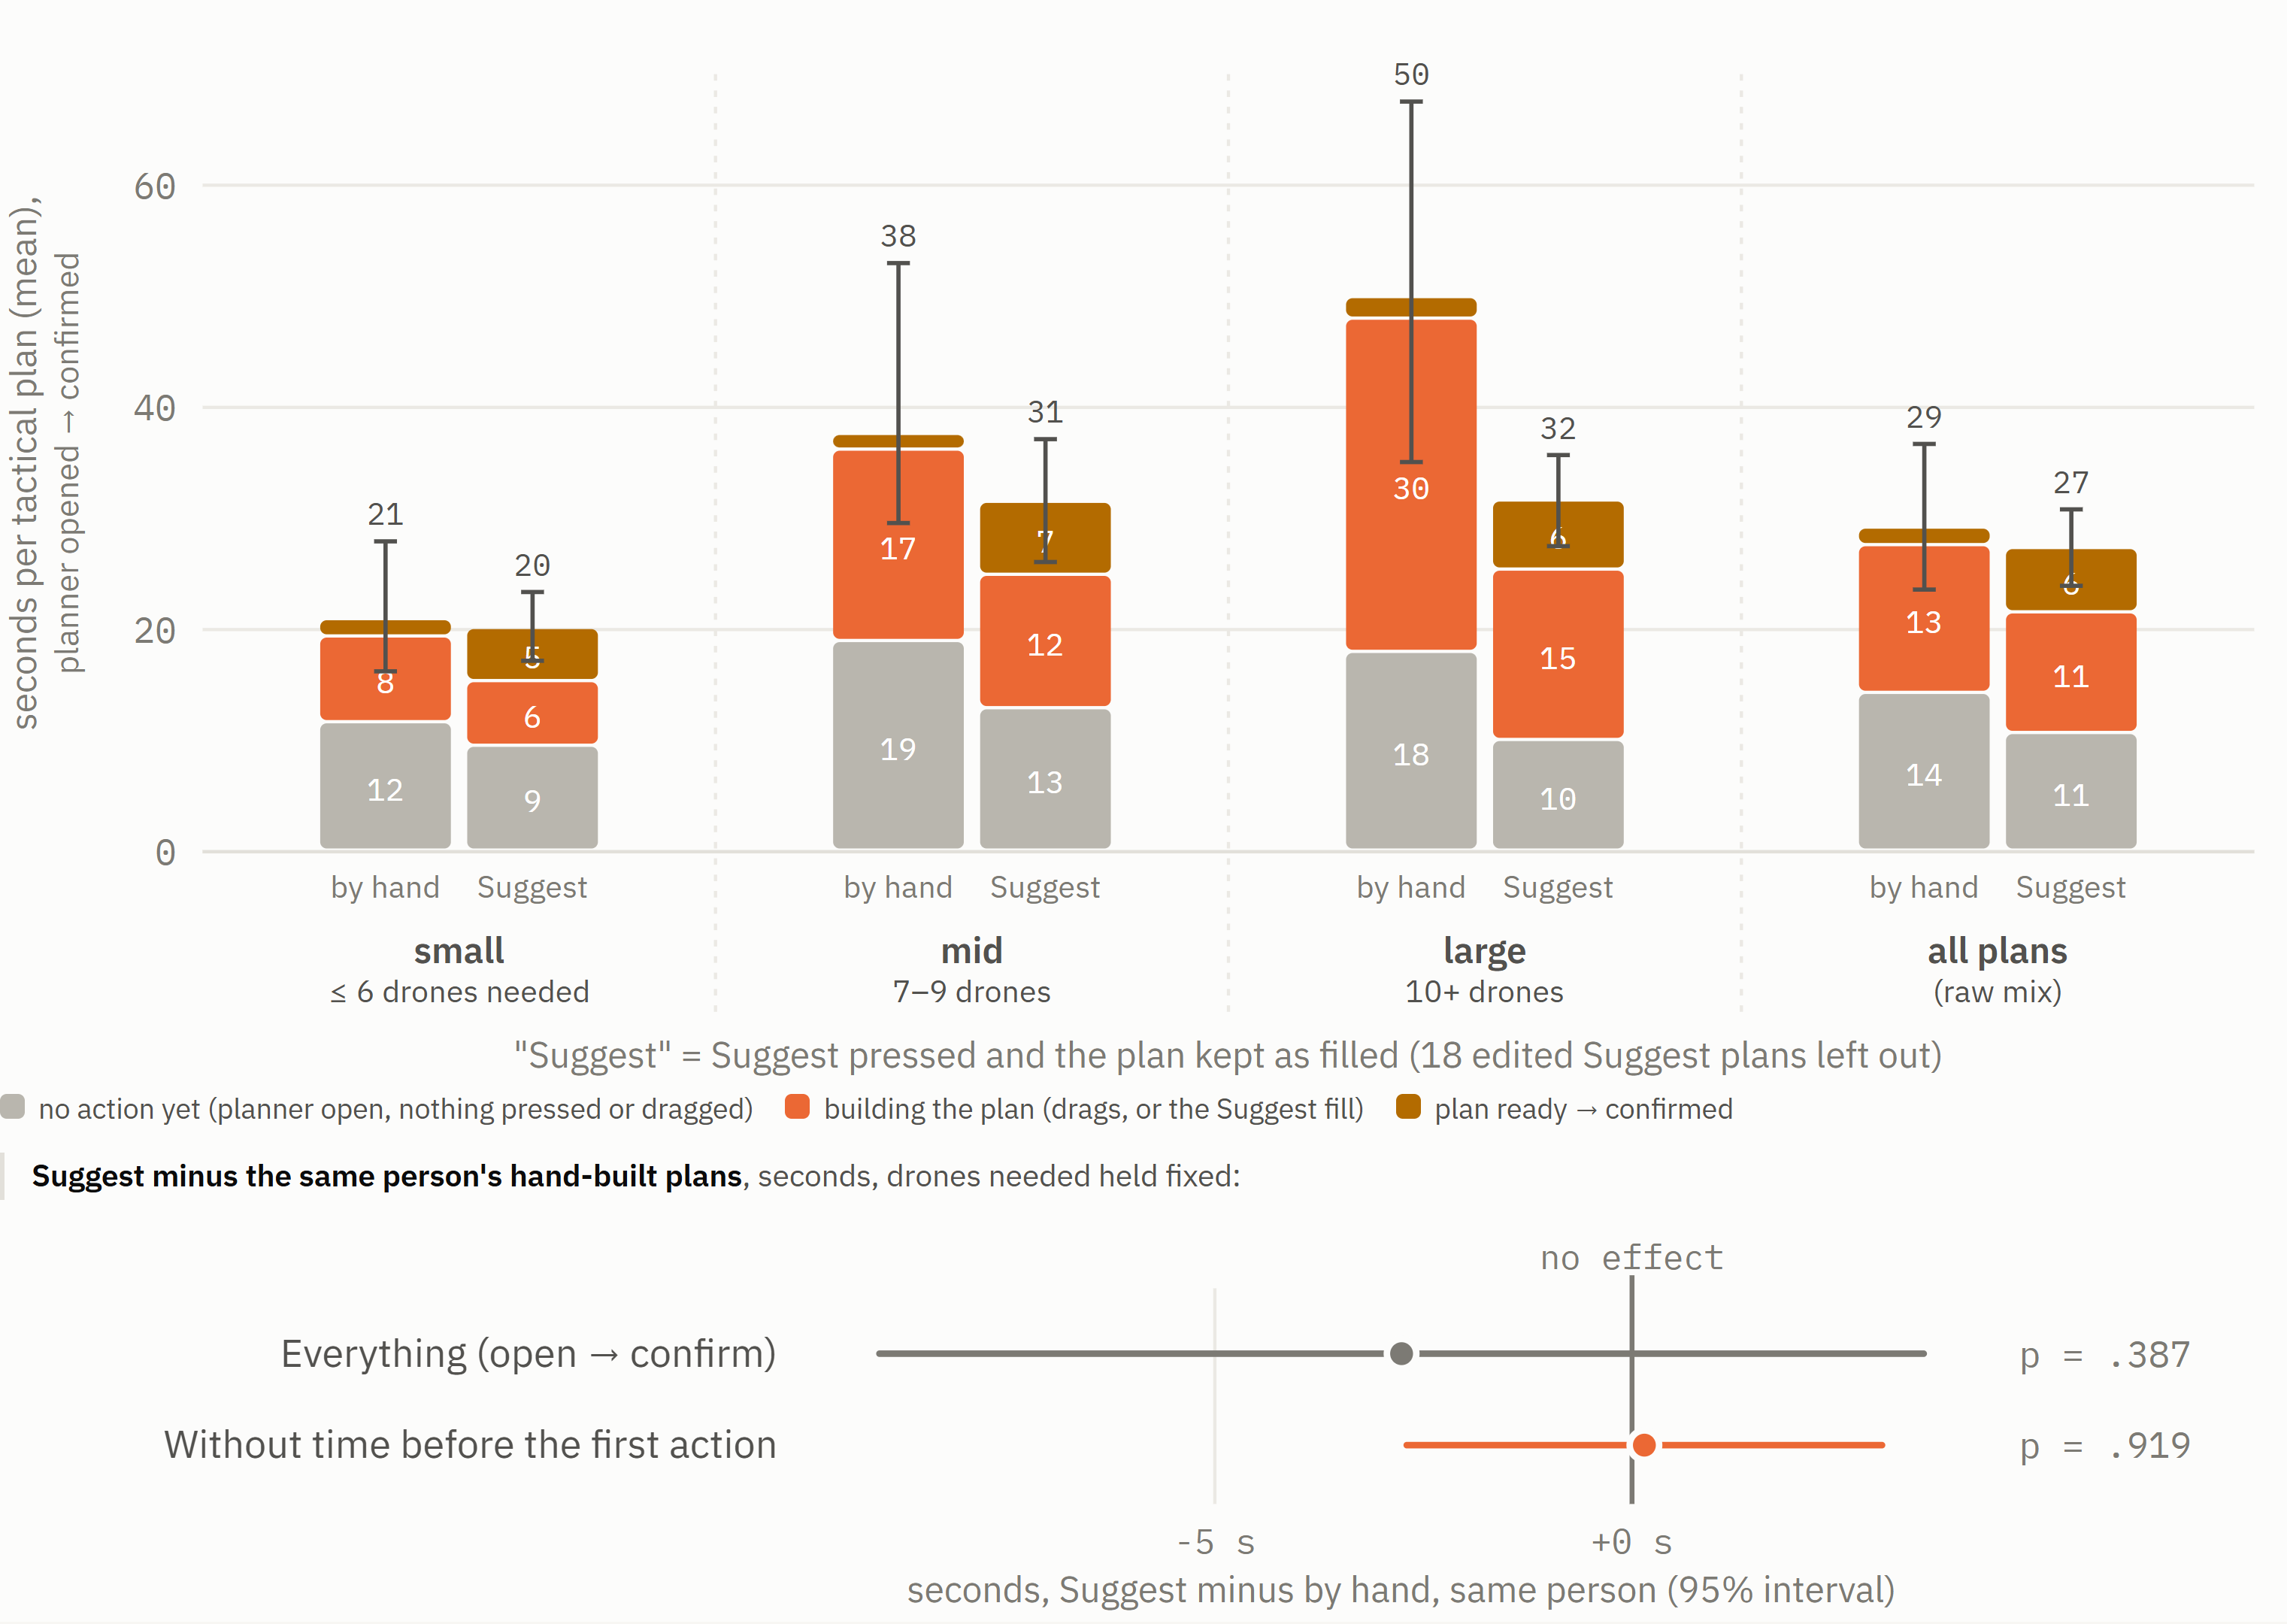
\includegraphics[width=\linewidth,height=0.23\textheight,keepaspectratio]{figs/results/f-size-decides__speed__tac-all.png}
\caption{Tactical tier, all time counted.}
\label{fig:res:size-decides:speed:tac-all}
\end{subfigure}
\hfill
\begin{subfigure}[t]{0.495\linewidth}
\centering
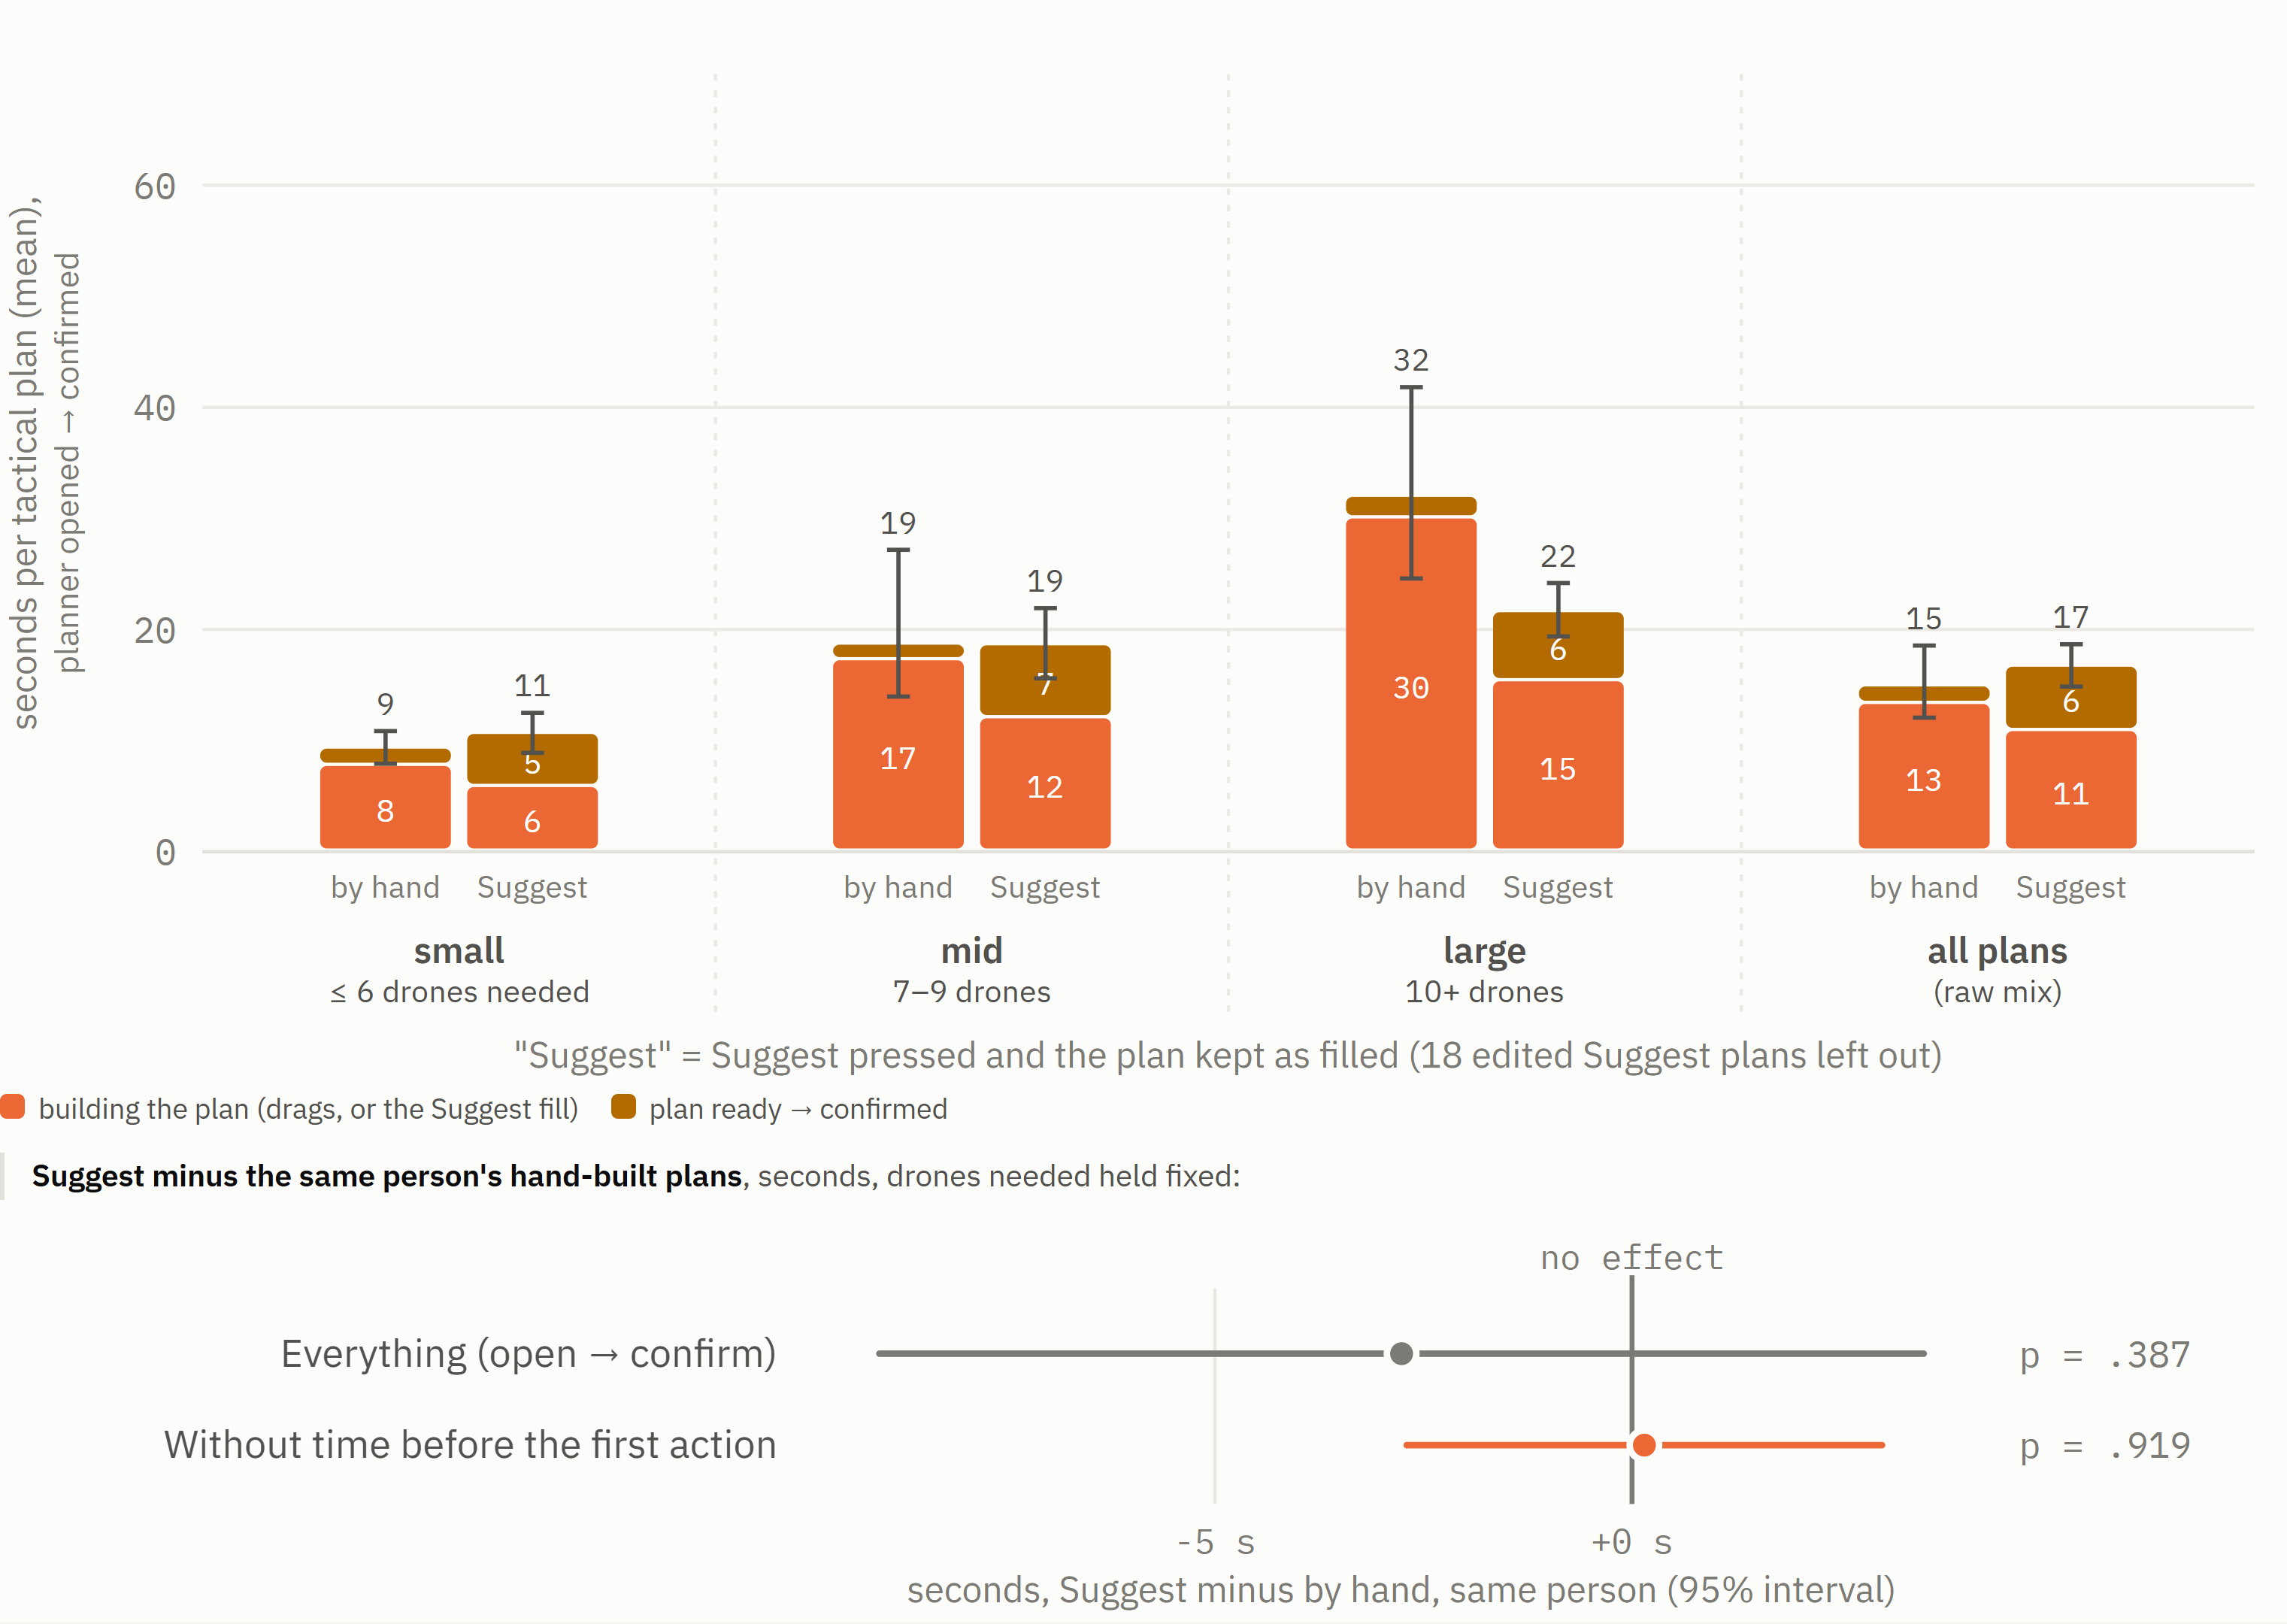
\includegraphics[width=\linewidth,height=0.23\textheight,keepaspectratio]{figs/results/f-size-decides__speed__tac-noidle.png}
\caption{Tactical tier, idle time removed.}
\label{fig:res:size-decides:speed:tac-noidle}
\end{subfigure}
\par\smallskip
\caption{\textbf{Why the rule makes sense: the card pays only on big strategic jobs; Suggest is not slower}}
\label{fig:res:size-decides:speed}
\end{figure}

\paragraph*{Key numbers.}

\begin{itemize}[leftmargin=1.2em,itemsep=1pt]

\item Strategic, card vs manual, same person, \% change in time: everything: one-type +22\% [$-$3, +55], p = .09; three-type $-$27\% [$-$35, $-$17], p < .001

\item Without idle time: one-type $-$8\% [$-$19, +4], p = .17; three-type $-$44\% [$-$49, $-$38], p < .001. From the first click only: one-type $-$40\%, three-type $-$76\% (both p < .001)

\item Strategic means (s), loading + idle + acting: one-type card 4.7 + 6.5 + 2.2 = 13.3; by hand after cards 4.7 + 8.6 + 5.0 = 18.2; before cards 3.7 + 0.7 + 3.0 = 7.4. Three-type 10--18 drones: card 4.6 + 7.3 + 2.1 = 14.0; by hand 4.6 + 10.1 + 9.7 = 24.4

\item Tactical means (s), idle + building + ready $\rightarrow$ confirmed: all plans by hand 14.2 + 13.3 + 1.6 = 29.1 (144) vs Suggest 10.6 + 10.9 + 5.8 = 27.2 (465); large missions 17.9 + 30.0 + 1.9 = 49.8 (22) vs 10.0 + 15.3 + 6.2 = 31.5 (159)

\item Tactical, Suggest minus by hand, same person, drones needed held: everything $-$2.8 s [$-$9.0, +3.5], p = .39; without idle time +0.2 s [$-$2.7, +3.0], p = .92; Suggest $\times$ size (without idle) $-$1.3 s per doubling, p = .47

\item Tactical plans idle for more than 10 s: 54\% had another mission's strategic panel opened before the first action (176 plans); all plans 22\%

\end{itemize}

\paragraph*{Method.} {\small \textbf{Rows}: strategic, the 606 card decisions (the last panel opening before the choice, as everywhere in this finding); tactical, the 627 non-recovery plans with a known mission size (kept Suggest plans vs hand-built; the 18 edited Suggest plans are in the table only). \textbf{Segments}, from the event log: strategic, panel opened $\rightarrow$ first click (split at the moment the cards appeared: before = ``cards still loading'', after = ``idle, cards on screen'') and first click $\rightarrow$ choice; tactical, planner opened $\rightarrow$ first Suggest press or drag (``idle''), $\rightarrow$ plan ready (last drag, or the end of the one-entry-per-second Suggest fill), $\rightarrow$ confirmed. These are the same phases as the next section, which adds carrying out. Bars are means (means add up, medians do not), whiskers 95\% intervals of the bar's total from resampling people. Sizes: strategic, one-type missions (3--6 drones) and three-type missions of 6--9 and 10--18 drones; tactical, drones needed $\leq$ 6, 7--9, 10+. \textbf{Models}: strategic, Gaussian GEE on log seconds, card $\times$ three-type, all manual decisions pooled as the comparison, the person's own card rate, drones, game, session and minute held fixed, run once per way of counting; tactical, GEE on seconds, Suggest split within/between person, drones needed, game and session fixed. \textbf{Caveat}: idle time mixes reading the cards or plan with being busy elsewhere, and the log cannot tell them apart. For tactical plans idle for more than 10 s, 54\% had another mission's strategic panel opened in that time, so long idle time is often attention elsewhere.}

\paragraph*{What participants said.} \regtext{Speed is the most common reason given for using the assistants: 15 of 33 coded C04. Many add that the plan is not better, just faster (P04, P17, P11). The card's loading wait is the main complaint. Six were coded C06, and in the think-aloud P18, P21, P29 and P32 go manual because they 'can't wait' for the cards, mostly on small missions. That matches the finding that the card pays off only on big strategic jobs. P20 first said the strategic assistant saved them more time, then corrected themself on remembering its loading stage.}

\paragraph*{Quotes selected for this section.}

\begin{quotelist}

\item ``I think the key strength when I [am] using the agent is it can help me to save the time and energy to those specific deployments''\,---\,P28 (debrief 0:32:10)

\item ``the point is, it takes me so much time to untangle that, that maybe it probably will not be faster if I do it myself manually. So as long as the AI makes sure that everything is covered once.''\,---\,P17 (think-aloud s1 0:07:07)

\item ``Manually, [I] can't wait for the processing, to be honest.''\,---\,P21 (think-aloud s1 0:09:32)

\item ``I think even if the tactical agent gave me a dodgy suggestion and the mission failed and I lost points, I probably would have gained more points from the time saved...''\,---\,P11 (debrief 0:30:11)

\item ``The top advantage in this situation was the speed of response.''\,---\,P31 (debrief 0:29:10)

\item ``I think I was definitely a bit slower than the, than the algorithm there.''\,---\,P22 (think-aloud s1 0:07:11)

\item ``You know, it's quicker to get a suggestion, but it is less clicking, and it seems to do what I would do.''\,---\,P32 (think-aloud s1 0:10:07)

\item ``So, it just seems quicker to just send some myself than wait for the recommendation. I might just be impatient.''\,---\,P32 (think-aloud s1 0:03:09)

\item ``So, when we are trying to do with the tactical screen, I find the agent is quite slow.''\,---\,P27 (debrief 0:29:10)

\item ``Yeah, when I located, I think sometimes the AI will take a little longer. And I just mess up my strategy''\,---\,P26 (debrief 0:28:37)

\end{quotelist}

\clearpage

\subsubsection{Where the tactical time goes: hand-built and Suggest plans are close, with a small edge to Suggest in carrying the plan out}\label{sec:res:size-decides:parallel}

\noindent \passtag{for the paper}

\noindent \regtext{Each tactical plan split into four phases: before the first action (idle, or busy elsewhere), building the plan (drags, or the one-entry-per-second Suggest fill), plan ready $\rightarrow$ confirmed, and carrying out (confirm $\rightarrow$ mission complete), for every size group side by side; the toggle leaves out the time before the first action. \textbf{The headline is how close the bars are.} The operator's own time on a plan is the same either way: Suggest saves about 3 s in building and gives it back waiting between ready and confirmed (net about +1 s). The only reliable difference is in carrying the plan out, about 11 s sooner for a Suggest plan (roughly a tenth of a mission's time), so the assistant's plans are very slightly better rather than much faster to make. Read the large group with care: only 6 hand-built large plans finished cleanly. The raw ``all missions'' bars look the other way (hand-built 90 s, Suggest 100 s); that is a mix effect, not a contradiction: 78\% of finished hand-built plans are small missions, against 42\% of Suggest plans. Given the same mix of sizes, hand-built plans take 109 s and Suggest 96 s. So the common feeling that the assistant is ``faster'' is only weakly supported: it does not save the operator time, and the plans it makes finish a little sooner. Each tier's use still looks sensible: Suggest is used where plans are big, which is where its small edge in execution adds up. And relying on the assistants more does not make an operator do better: within a person, card missions are completed in full no more often than their own hand-built ones (odds $\times$0.81, p = .27; raw 60\% vs 62\%), and session score is flat in sessions where they rely more ($-$0.10 SD per 25 points of card uptake, p = .61). The ready $\rightarrow$ confirmed gap is when operators turn to other missions: 45\% of Suggest plans had another mission's strategic panel opened while the planner was open, against 19\% of hand-built ones.} (Figure~\ref{fig:res:size-decides:parallel})

\begin{figure}[H]
\centering
\begin{subfigure}[t]{\linewidth}
\centering
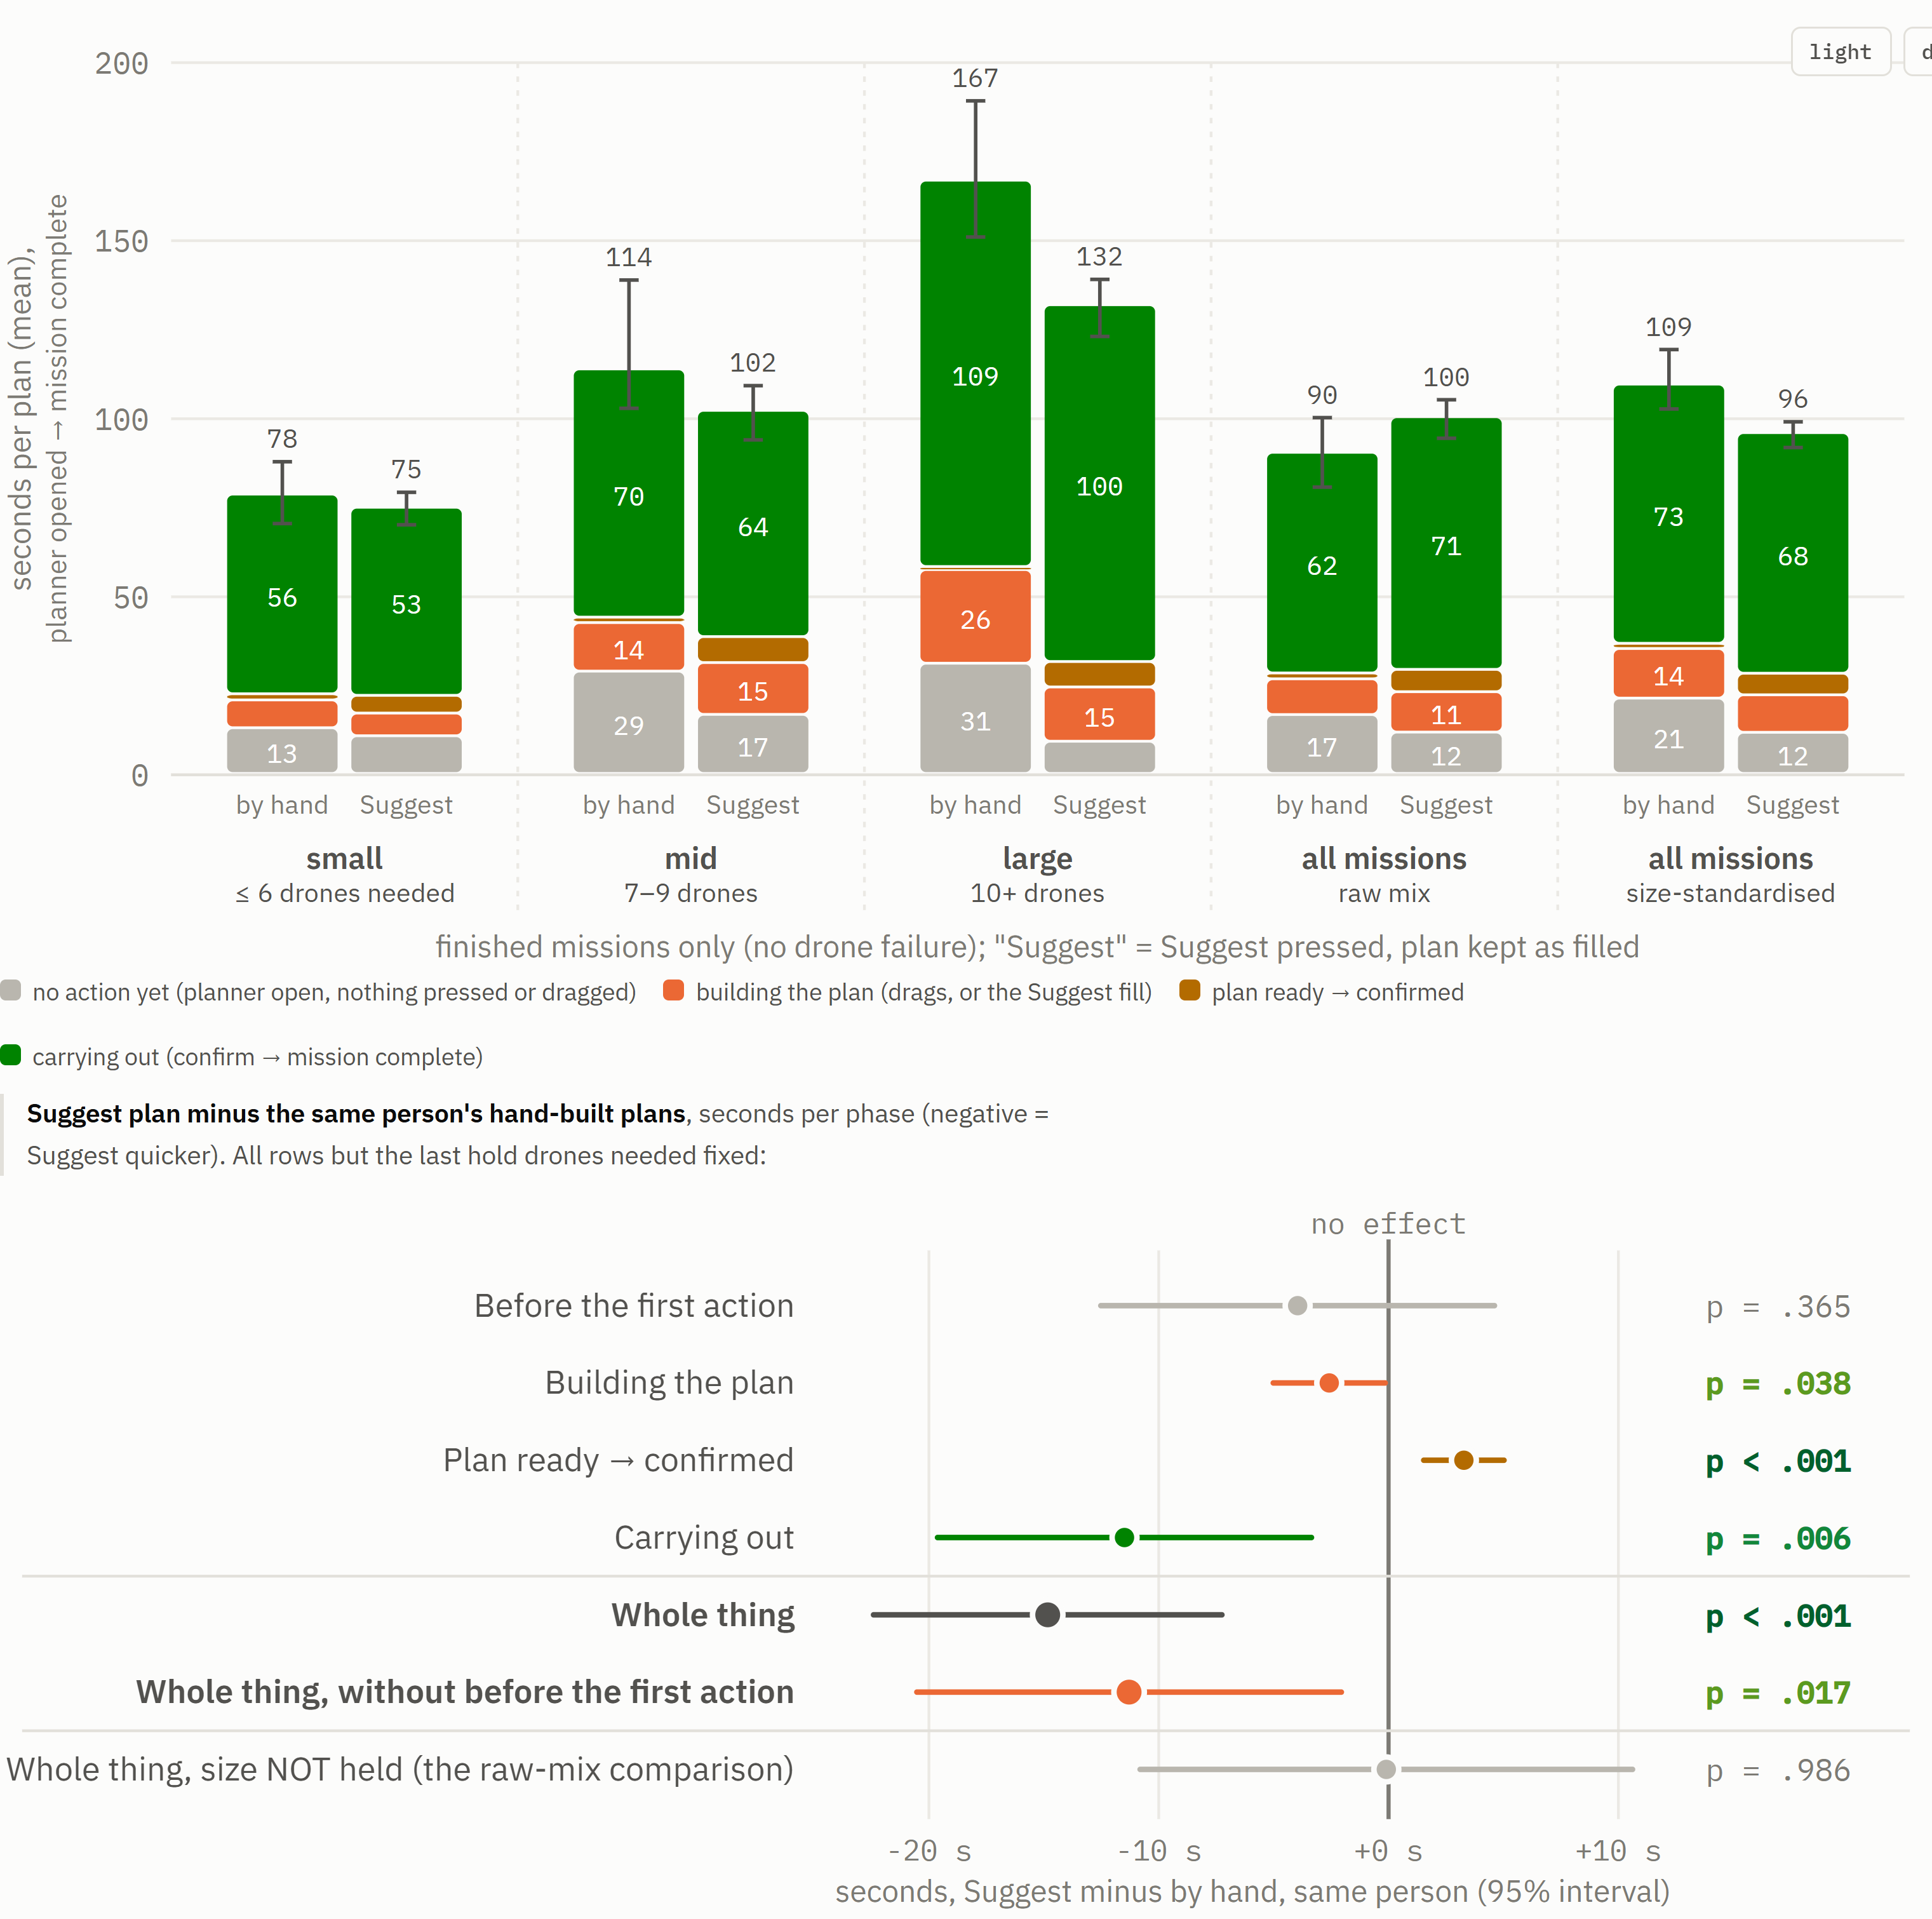
\includegraphics[width=\linewidth,height=0.23\textheight,keepaspectratio]{figs/results/f-size-decides__parallel__all.png}
\caption{All four phases.}
\label{fig:res:size-decides:parallel:all}
\end{subfigure}
\par\smallskip
\begin{subfigure}[t]{\linewidth}
\centering
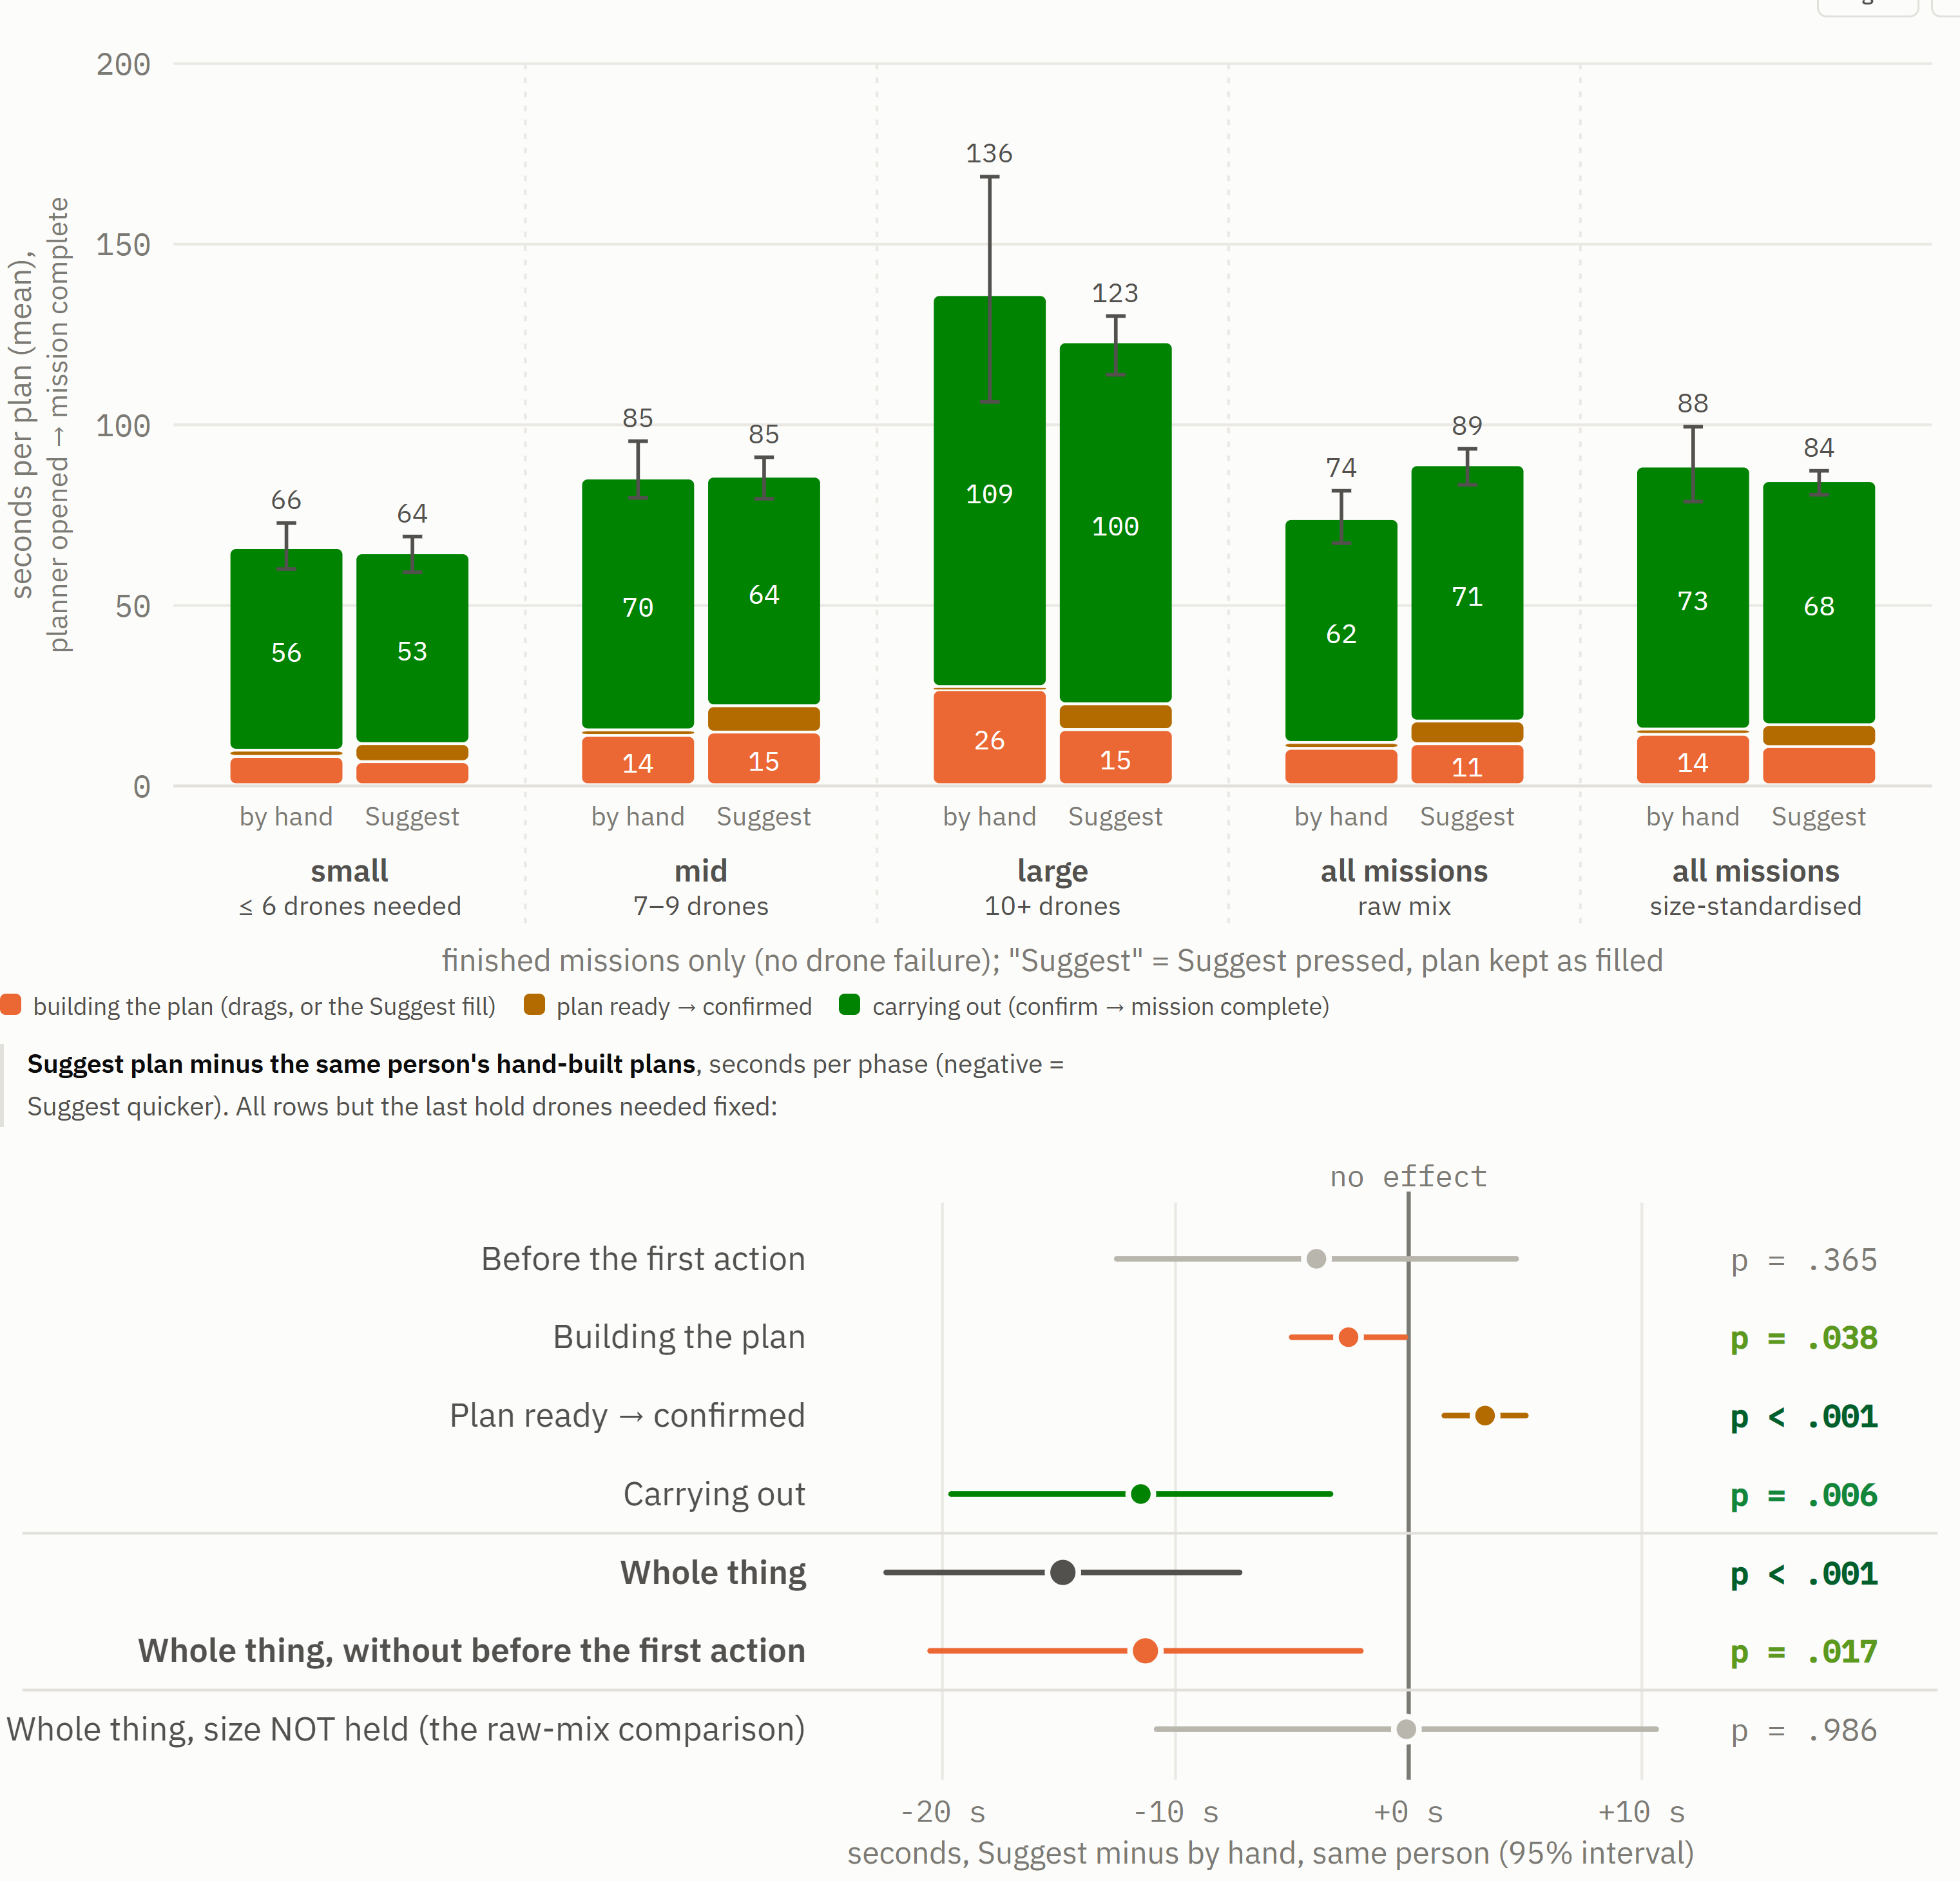
\includegraphics[width=\linewidth,height=0.23\textheight,keepaspectratio]{figs/results/f-size-decides__parallel__noidle.png}
\caption{Without the time before the first action.}
\label{fig:res:size-decides:parallel:noidle}
\end{subfigure}
\par\smallskip
\caption{\textbf{Where the tactical time goes: hand-built and Suggest plans are close, with a small edge to Suggest in carrying the plan out}}
\label{fig:res:size-decides:parallel}
\end{figure}

\paragraph*{Key numbers.}

\begin{itemize}[leftmargin=1.2em,itemsep=1pt]

\item Suggest minus hand-built, same person, drones needed held (315 finished plans): before the first action $-$4.0 s [$-$12.5, +4.6], p = .37; building $-$2.6 s [$-$5.0, $-$0.1], p = .038; ready $\rightarrow$ confirmed +3.3 s [+1.5, +5.0], p < .001; carrying out $-$11.5 s [$-$19.6, $-$3.4], p = .006; whole $-$14.8 s [$-$22.4, $-$7.3], p < .001

\item Whole thing without the time before the first action: $-$11.3 s [$-$20.5, $-$2.1], p = .017; whole thing with size not held: $-$0.1 s [$-$10.8, +10.6], p = .99

\item Means (s), hand vs kept Suggest: small 78.5 vs 74.8 (63 vs 97 plans); mid 113.6 vs 102.0 (12 vs 59); large 166.6 vs 131.6 (6 vs 75); all, raw 90.2 vs 100.2; all, size-standardised 109.3 [102.7, 119.4] vs 95.7 [91.9, 99.1]

\item Size mix of finished plans: hand-built 78\% small, 15\% mid, 7\% large (mean 5.7 drones needed); Suggest 42\%, 26\%, 32\% (mean 8.8)

\item All 627 plans, first three phases: before $-$2.9 s, p = .29; building $-$3.2 s [$-$6.2, $-$0.1], p = .04; ready $\rightarrow$ confirmed +3.3 s [+2.0, +4.6], p < .001

\item Carrying out, including missions with a drone failure (378): $-$8.1 s [$-$17.1, +0.9], p = .08: same direction, less certain

\item Projected completion vs the assistant's own plan at open, median: hand-built +10.3 s [3.7, 28.3] (144 plans), kept Suggest +1.6 s [0.8, 4.0] (468), edited Suggest +38.7 s (18)

\item Interleaving, round-1 specification re-run: odds $\times$4.83 [2.24, 10.40], p < .001 (630 plans, 33 people); raw 45\% vs 19\%; 28\% vs 11\% actually allocated another mission

\item Operator time, building + ready $\rightarrow$ confirmed, Suggest minus hand-built, same person, size held: $-$2.6 s + 3.3 s $\approx$ +0.7 s (negligible)

\item From the retired ``who does better'' finding: within a person, card missions vs own manual missions, completed in full odds $\times$0.81 [0.55, 1.18], p = .27 (raw 60\% vs 62\%); session score per +25 points of card uptake $-$0.10 SD [$-$0.47, 0.27], p = .61. Between people, heavier card users complete more ($\times$1.32 per 25 points, p = .004): the difference is in the people, not the advice

\end{itemize}

\paragraph*{Method.} {\small \textbf{Rows}: confirmed non-recovery tactical plans. \textbf{Phases} from the event log, the same as in section 4: planner opened (\emph{tactical\_opened}); first action = first Suggest press or first drag; plan ready = last drag, or for a Suggest plan the end of its fill (last press + 1 s per drone-task entry), whichever is later; confirmed (\emph{tactical\_confirmed}); mission complete (\emph{mission\_completed}). \textbf{Carrying out} can only be measured when the mission finished in full with no drone failure: 315 of 630 plans; the chart shows those (81 hand-built, 231 kept Suggest; edited Suggest plans left out, 3 survive). Size groups by drones needed: small $\leq$ 6, mid 7--9, large 10+. Bars are means, whiskers 95\% intervals of the bar's total from resampling people. \textbf{Size-standardised}: each route's mean in each size group, weighted by the share of all finished plans in that group (small 51\%, mid 23\%, large 26\%), so both routes get the same mix; this answers ``how long would each route take on the same missions?''. Only 6 large hand-built plans finished cleanly (5 people), so that bar and the standardised hand-built bar are the least certain. \textbf{Model}: Gaussian GEE of seconds in each phase on ``Suggest pressed'' (split within/between person), log drones needed, game and session. Seconds add up, so the phase differences sum to roughly the whole. The bottom row drops drones needed from the model: still within person, but with size not held the difference vanishes ($-$0.1 s), which shows the raw reversal comes from size, not from who uses which route. \textbf{Projected completion} and \textbf{interleaving} as before.}

\clearpage

\subsubsection{What operators say}\label{sec:res:size-decides:said}

\noindent \passtag{for the paper}

\noindent \regtext{Ten of 33 state the rule unprompted (C03: small/simple myself, big/complex to the assistant); 15 value the assistant for speed rather than accuracy (C04, the most common reason given); 8 describe working on something else while it runs (C05). The behaviour matches the words. People who state the rule press Suggest less overall (59\% vs 86\% of plans) and their size slope is, if anything, steeper on the tactical tier ($\times$1.43 steeper, p = .10) --- not reliably different from everyone else's, so stating the rule is not what makes someone follow it.}

\paragraph*{Key numbers.}

\begin{itemize}[leftmargin=1.2em,itemsep=1pt]

\item C03 10 of 33; C04 15 of 33; C05 8 of 33

\item C03 vs others, size slope ratio: strategic $\times$1.28 [0.69, 2.38], p = .43; tactical $\times$1.43 [0.93, 2.20], p = .10

\end{itemize}

\paragraph*{Method.} {\small Codes from the qualitative coding (docs/analysis/qual/codes\_matrix.csv); excerpts are pulled by code on the page. Slope comparison: the within-person size model with a size $\times$ C03 term (ratio of the two groups' odds ratios).}

\paragraph*{What participants said.} \regtext{10 of 33 state the size rule unprompted (C03), 15 value the assistant for speed rather than accuracy (C04) and 8 work in parallel (C05). The clearest statements tie all three together: small jobs are quicker by hand, big ones are a 'computation problem', and the wait frees attention for the next mission. Dissent from P30, P20 and P29 is in the first section. P32 said their use followed workload, not how hard a mission looked.}

\clearpage

\subsubsection{In their words: working in parallel while the assistant plans}\label{sec:res:size-decides:parallel-said}

\noindent \passtag{extra: may make it in}

\noindent \regtext{To close the finding: what people said about pressing Suggest and turning to other work while it fills in. It sits here rather than under the time-phase chart because it is about how people used the assistant, not about the chart's numbers.}

\paragraph*{What participants said.} \regtext{8 of 33 describe starting Suggest and working elsewhere while it fills in (C05). The think-aloud shows more of it (P19, P32, P36). Nobody said a Suggest plan finishes the mission sooner. Two people said the opposite about plan quality: P31 adjusted a Suggest plan they thought visited tasks in a poor order, and P21 found it lacked the cross-task redundancy they built themself.}

\clearpage

\subsection{Manual allocations are anchored on the cards --- and the 'trimming small missions' was mostly dropping the illogical spare}\label{sec:res:manual-cards}

\regtext{\textbf{Summary.} When operators allocate by hand after seeing the cards, their numbers track the cards: one more drone on the Conservative card means about half a drone more in the manual build, beyond what the mission needs. Operators who decided before the cards appeared show no such link --- a clean control, so this is anchoring, not both tracking the mission. Manual builds sit at or below the cards (44\% below both, 33\% equal to one, 14\% between, 8\% above). The earlier ``trim small missions, pad big ones'' mostly dissolves: on one-type missions the 'trim' is almost entirely dropping the Conservative card's spare drones of types the mission does not need.} \par\noindent{\small\textit{Strength of evidence (register rating): moderate. Your verdict: keep.}}

\subsubsection{Each manual decision against the Conservative card}\label{sec:res:manual-cards:dots}

\noindent \passtag{for the paper}

\noindent \regtext{Every manual allocation (209) as one dot: drones committed minus drones on the Conservative card, against the drones the mission needs. Switch to ``needed types only'' and the band of one-type missions moves up to zero: on the types the mission actually needs, manual builds on small missions match the Conservative card (+0.05 drones on average); the $-$1.2 drones on all types is the card's spare of each unneeded type being left off. On big three-type missions manual builds sit about one drone above the Conservative card (and still far below the drones the mission lists, since drones are reused across tasks in series).} (Figure~\ref{fig:res:manual-cards:dots})

\begin{figure}[H]
\centering
\begin{subfigure}[t]{\linewidth}
\centering
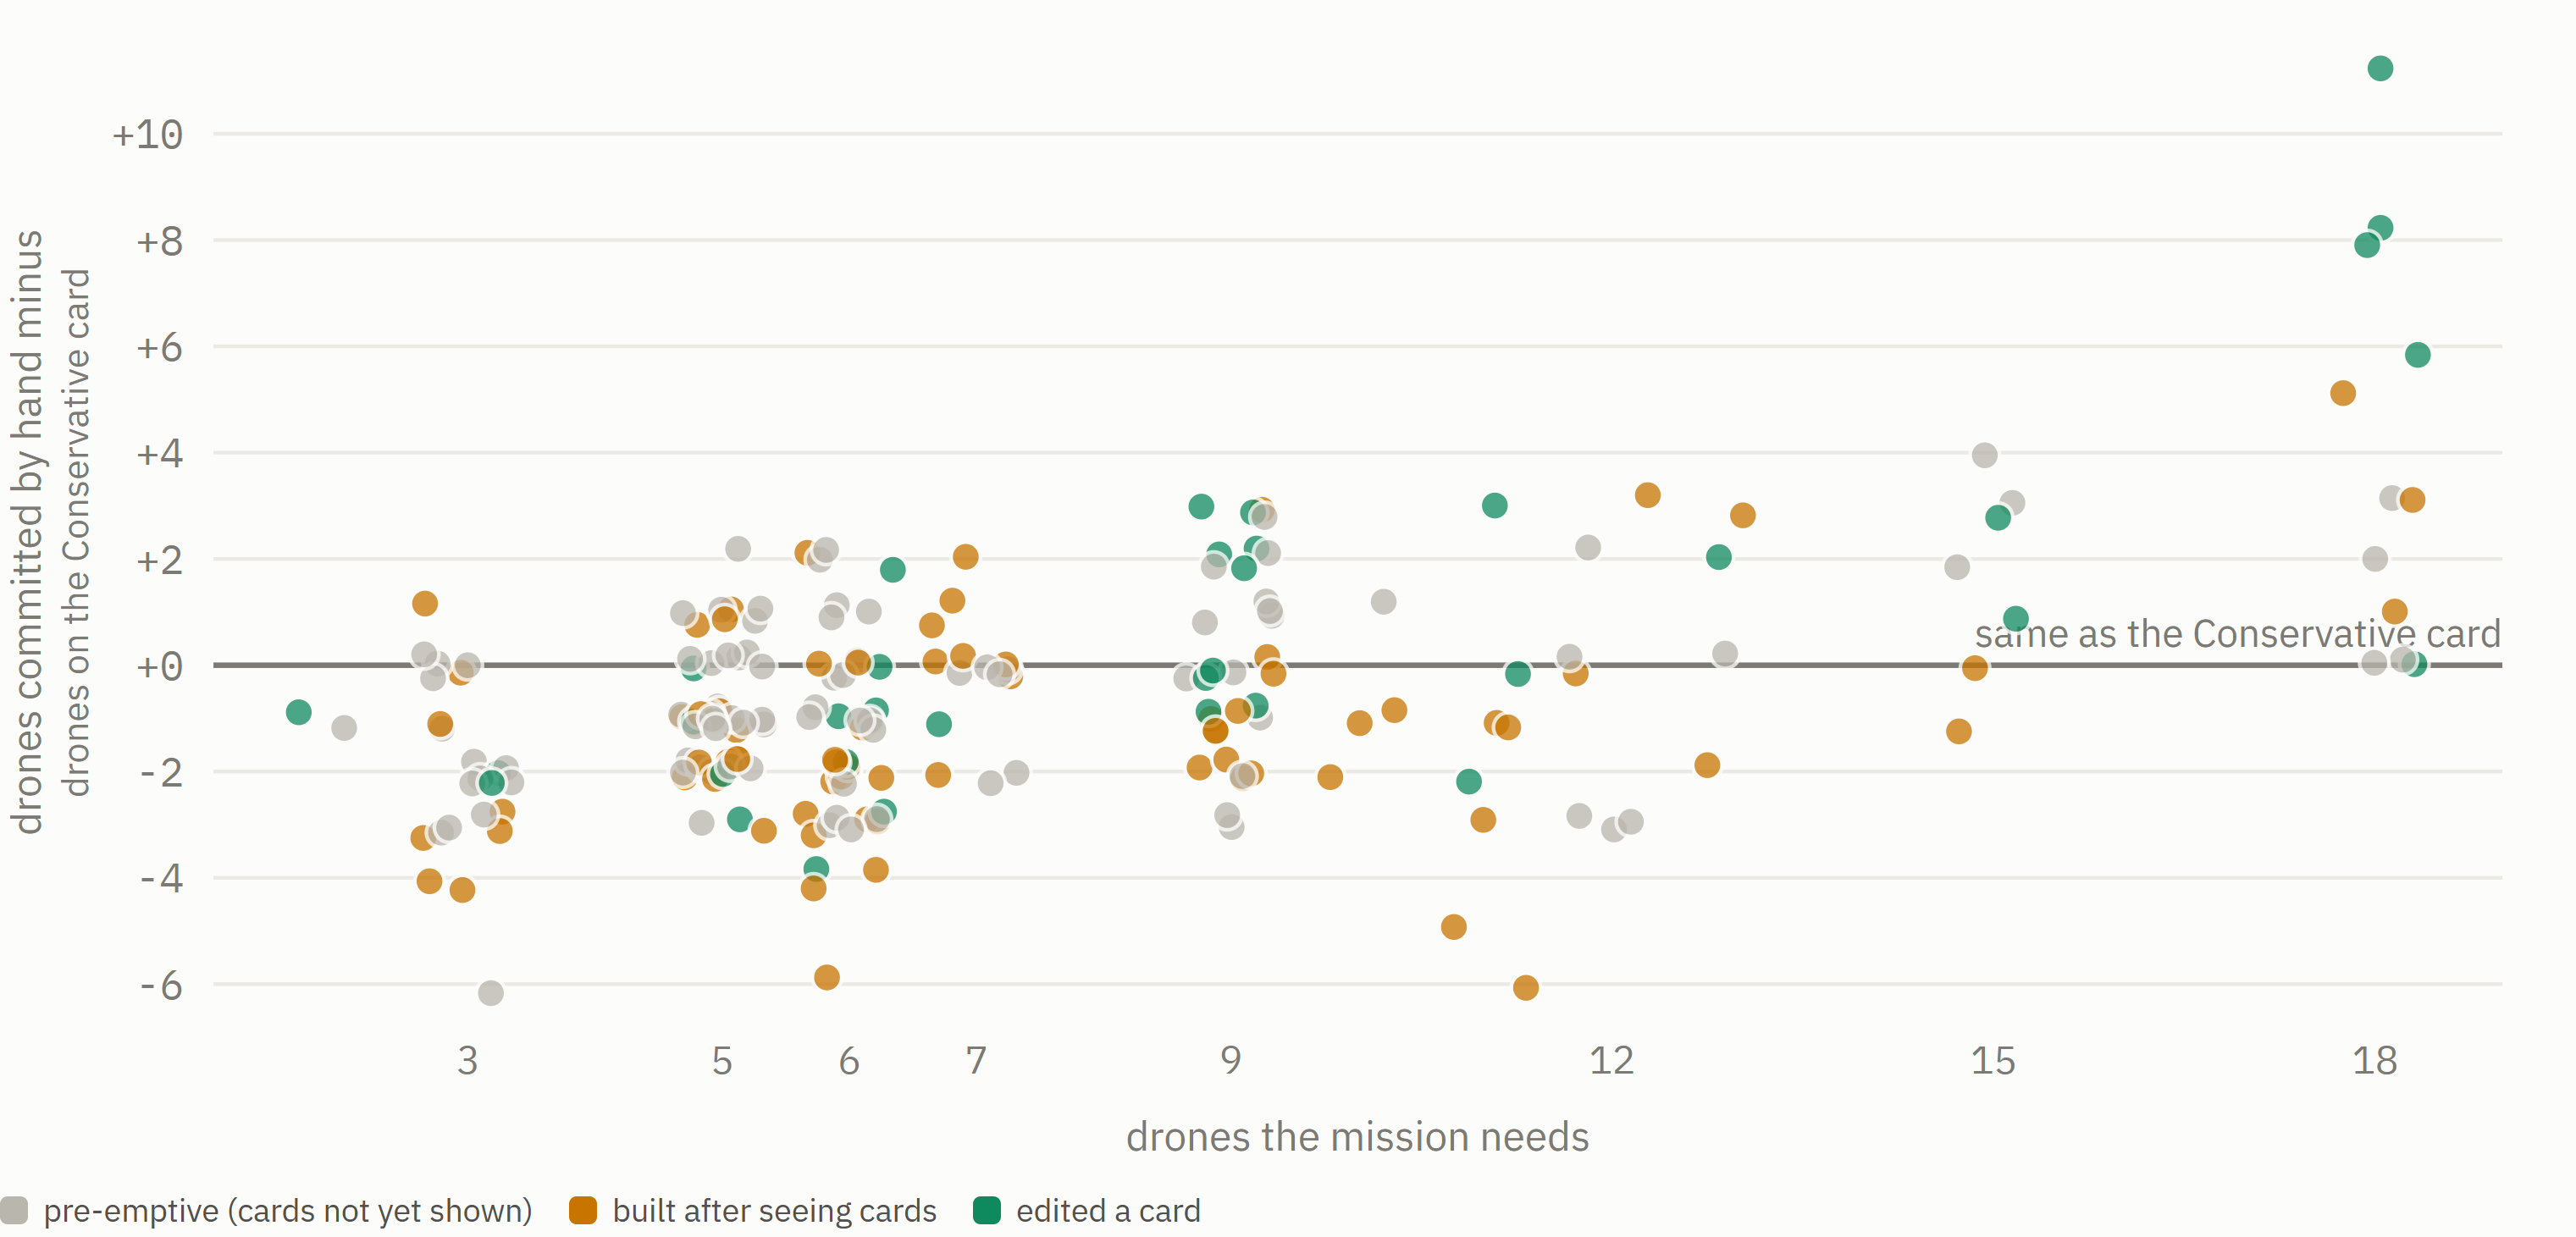
\includegraphics[width=\linewidth,height=0.23\textheight,keepaspectratio]{figs/results/f-manual-cards__dots__all.png}
\caption{All drone types.}
\label{fig:res:manual-cards:dots:all}
\end{subfigure}
\par\smallskip
\begin{subfigure}[t]{\linewidth}
\centering
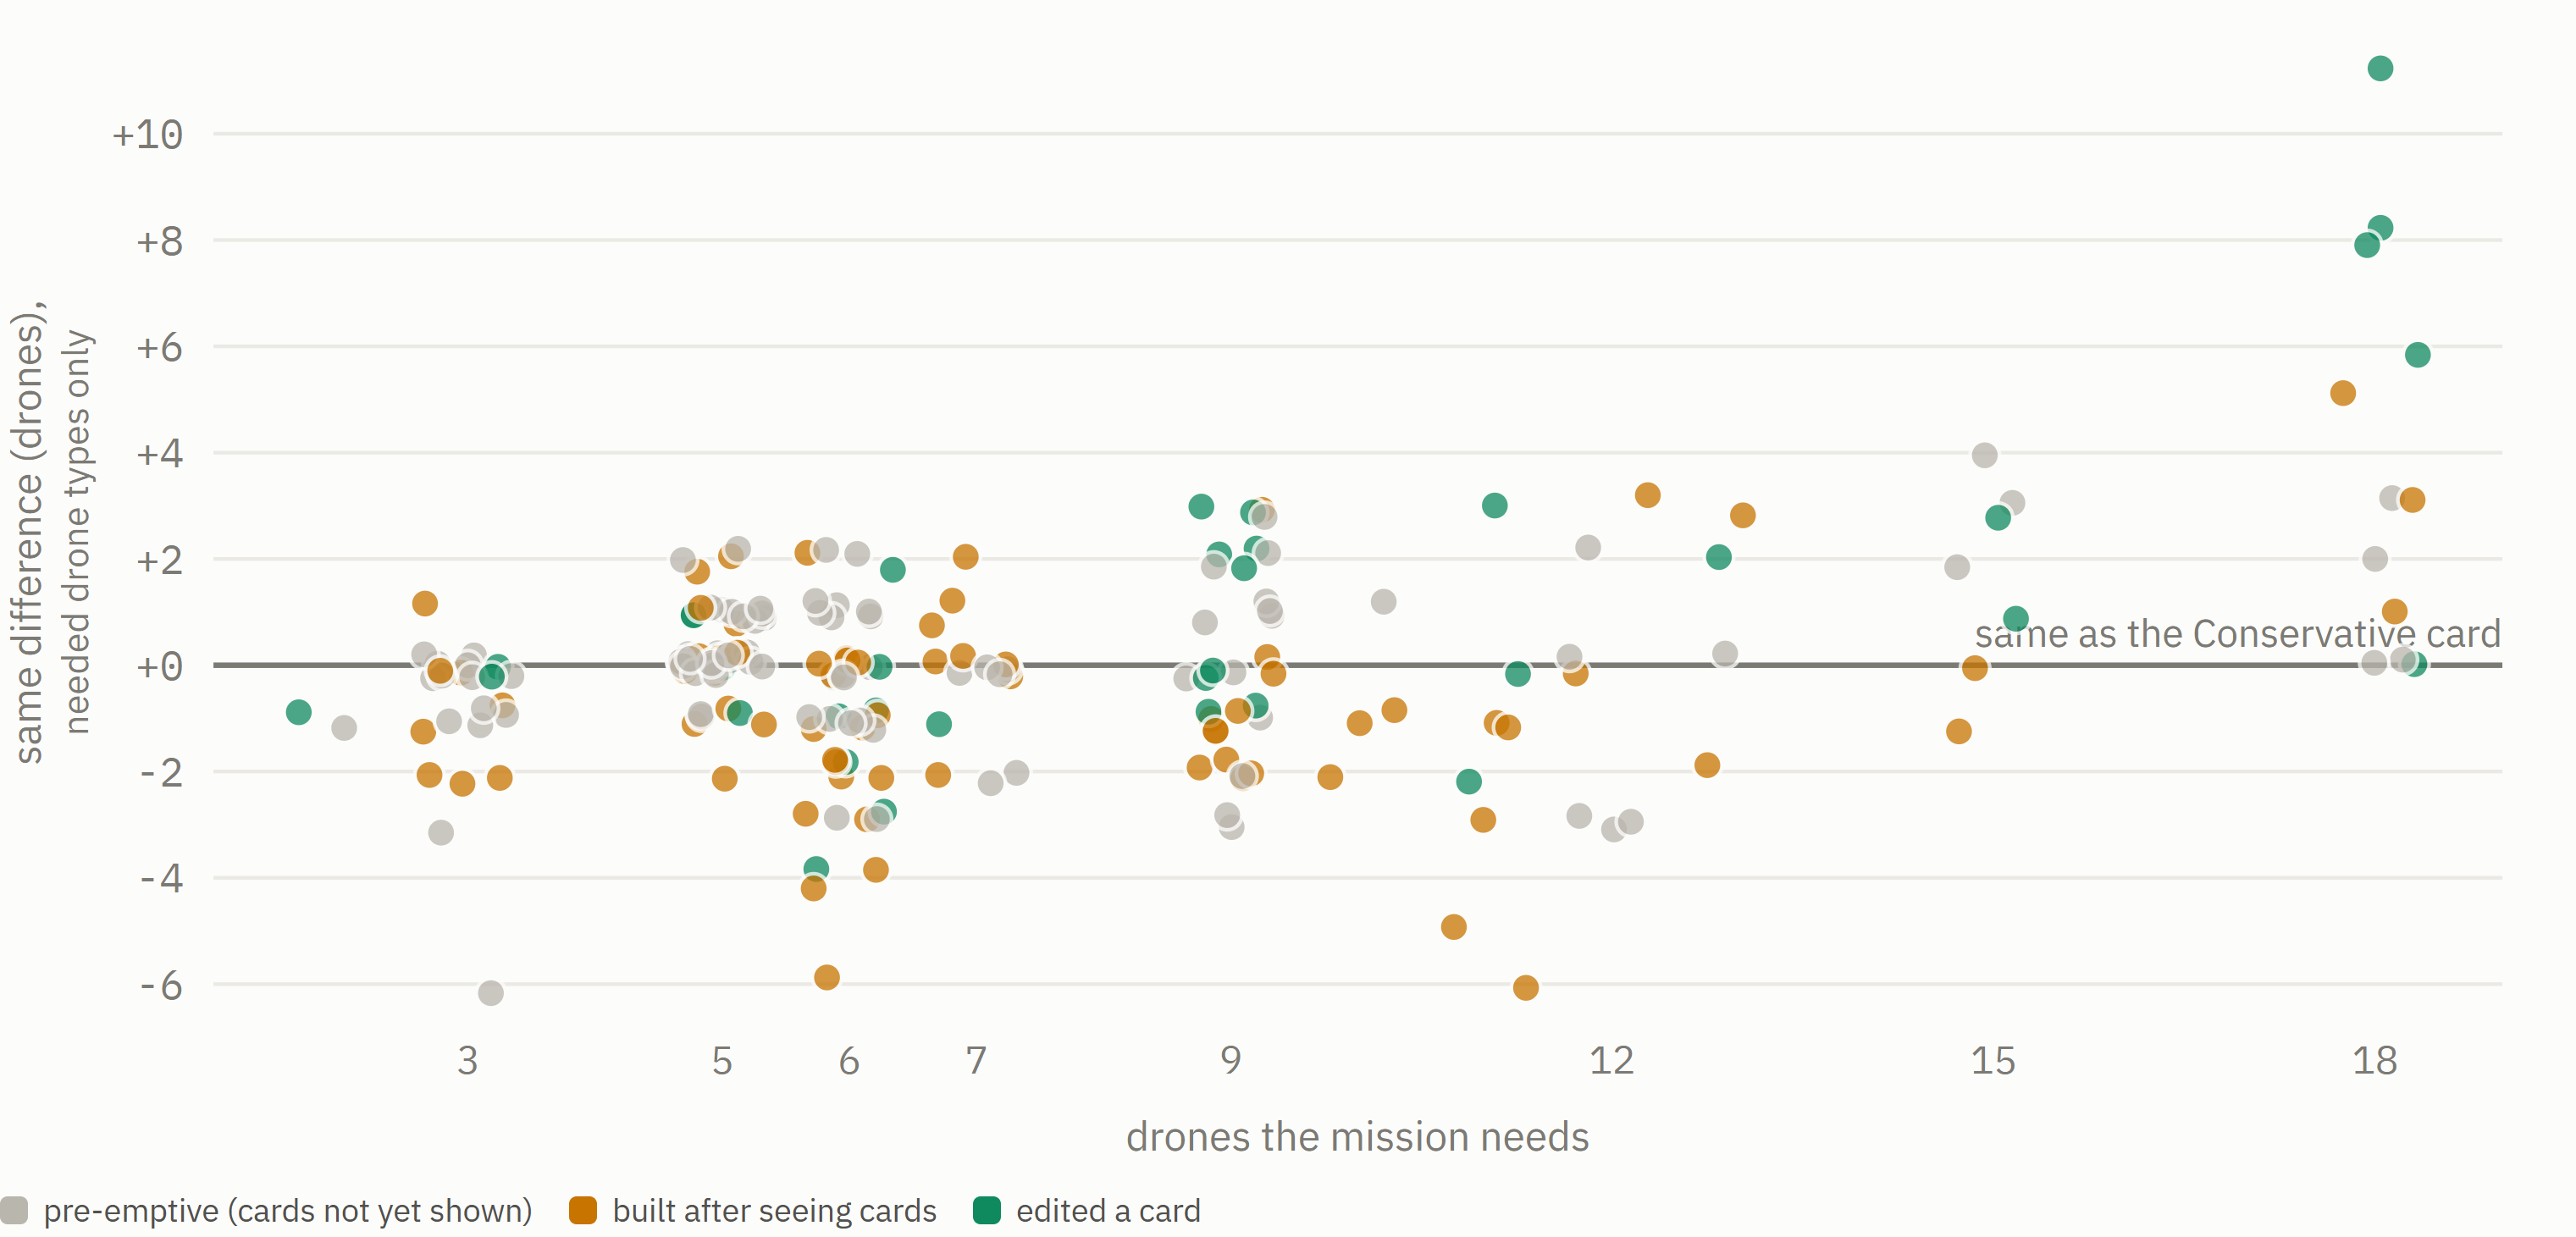
\includegraphics[width=\linewidth,height=0.23\textheight,keepaspectratio]{figs/results/f-manual-cards__dots__needed.png}
\caption{Needed drone types only.}
\label{fig:res:manual-cards:dots:needed}
\end{subfigure}
\par\smallskip
\caption{\textbf{Each manual decision against the Conservative card}}
\label{fig:res:manual-cards:dots}
\end{figure}

\paragraph*{Key numbers.}

\begin{itemize}[leftmargin=1.2em,itemsep=1pt]

\item Mean manual $-$ Conservative: $-$0.55 drones overall = $-$0.51 on unneeded types + $-$0.04 on needed types

\item One-type missions: $-$1.17 overall, +0.05 on needed types, $-$1.22 on unneeded; three-type with 10+ drones: +0.95

\item Per doubling of mission size the difference grows by +1.51 drones [0.53, 2.49] (after seeing the cards) and +1.09 [0.47, 1.72] (pre-emptive): the size pattern is just as strong in people who never saw the cards, so it is not a reaction to the card

\item Needed types only, after seeing the cards: +0.93 per doubling [$-$0.18, 2.04], p = .10

\end{itemize}

\paragraph*{Method.} {\small Rows: strategic choices of type manual. The cards' true asset counts per colour come from the last \emph{strategic\_modal\_opened} before the choice; the operator's counts from \emph{assetsChosen}. ``Needed types'' = colours with a primary requirement in the mission. Kinds: pre-emptive (decided before the cards loaded --- the cards existed in the log but were never on screen), edited a card (started from a card, then changed it), built after seeing the cards. Size slope: Gaussian within-person GEE of the difference on log2 drones needed.}

\paragraph*{What participants said.} \regtext{The think-aloud shows what was happening on the cards. People trimming small missions mostly said they were removing the card's drones of types the mission did not need (P10, P19, P21, P29, P13). Others cut one or two drones to protect the reserve (P24, P28). P20 shows the anchoring directly: they take the Aggressive card's numbers and does 'one less than each of those'. On big missions short of drones, P10 'send[s] everything I have', above the cards. One dissent: P29 found their own leaner builds sometimes had to be aborted.}

\paragraph*{Quotes selected for this section.}

\begin{quotelist}

\item ``All right. Let's just send everything I have. Edit, give me five red ones. Five green ones. Hit it.''\,---\,P10 (think-aloud s2 0:17:46)

\item ``I'm trying to reserve more and more drones in the base, rather than send them out to finish the task quickly, because I cannot predict when the next task will appear.''\,---\,P28 (debrief 0:28:05)

\end{quotelist}

\clearpage

\subsubsection{Where manual builds sit relative to the two cards}\label{sec:res:manual-cards:position}

\noindent \passtag{for the paper}

\noindent \regtext{Mostly below both cards or equal to one of them, rarely above. Pre-emptive builds --- made without seeing the cards --- land equal to a card total more often than builds made after seeing them (39\% vs 27\%), so 'equal to a card' is partly just the obvious allocation, not copying. Part of that gap is the missions: pre-emptive builds were on smaller, more often one-type missions. Balanced for the mission (second view), it is 37\% vs 29\%, too close to tell apart.} (Figure~\ref{fig:res:manual-cards:position})

\begin{figure}[H]
\centering
\begin{subfigure}[t]{\linewidth}
\centering
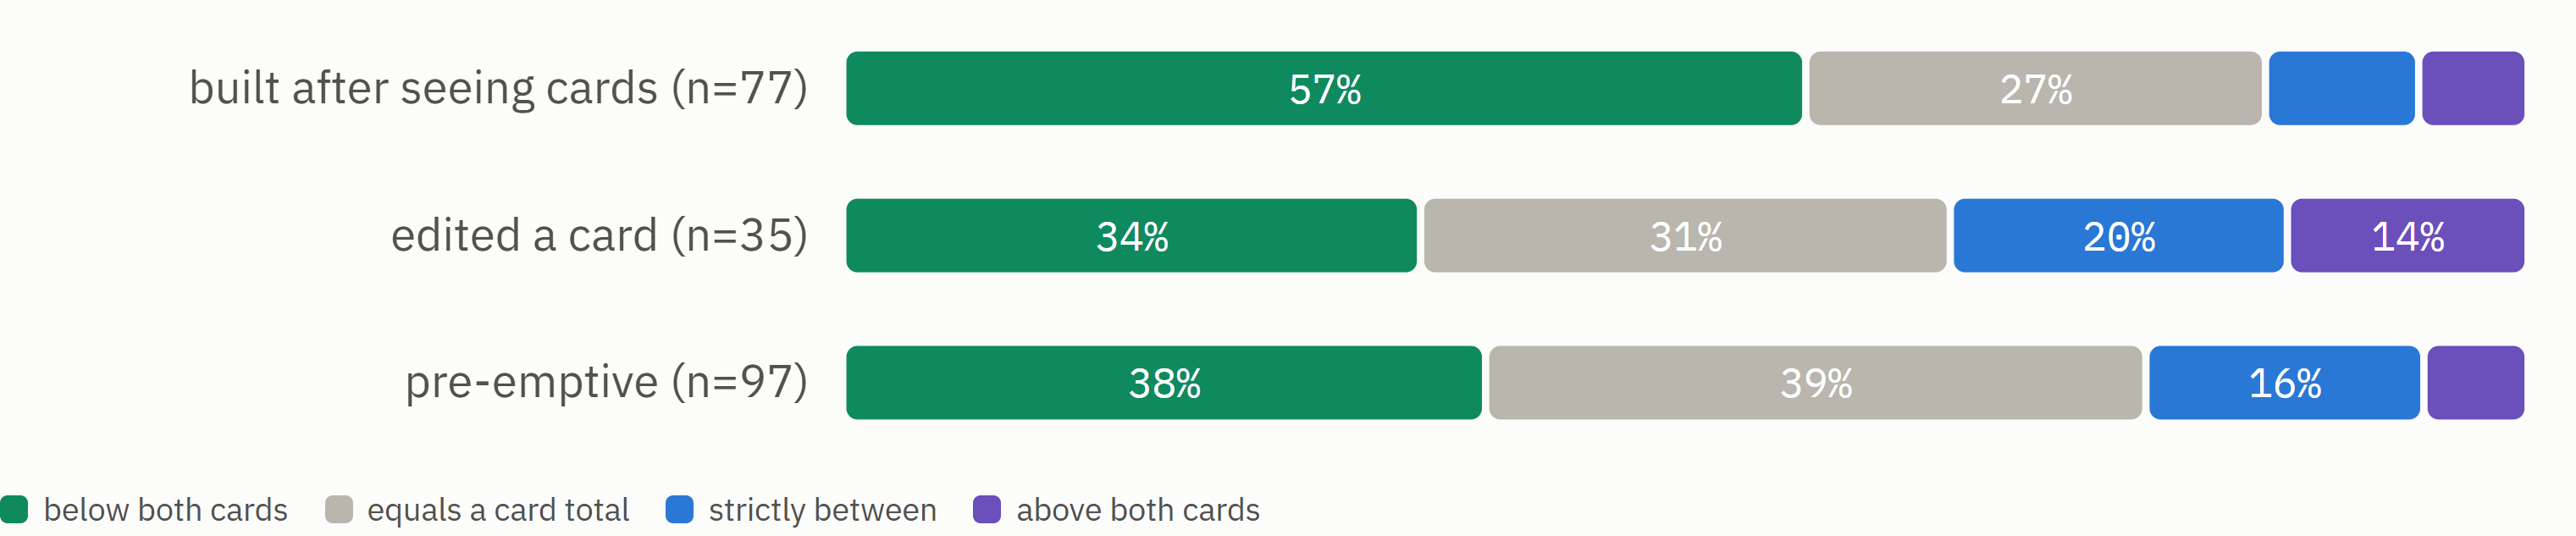
\includegraphics[width=\linewidth,height=0.23\textheight,keepaspectratio]{figs/results/f-manual-cards__position__raw.png}
\caption{As built.}
\label{fig:res:manual-cards:position:raw}
\end{subfigure}
\par\smallskip
\begin{subfigure}[t]{\linewidth}
\centering
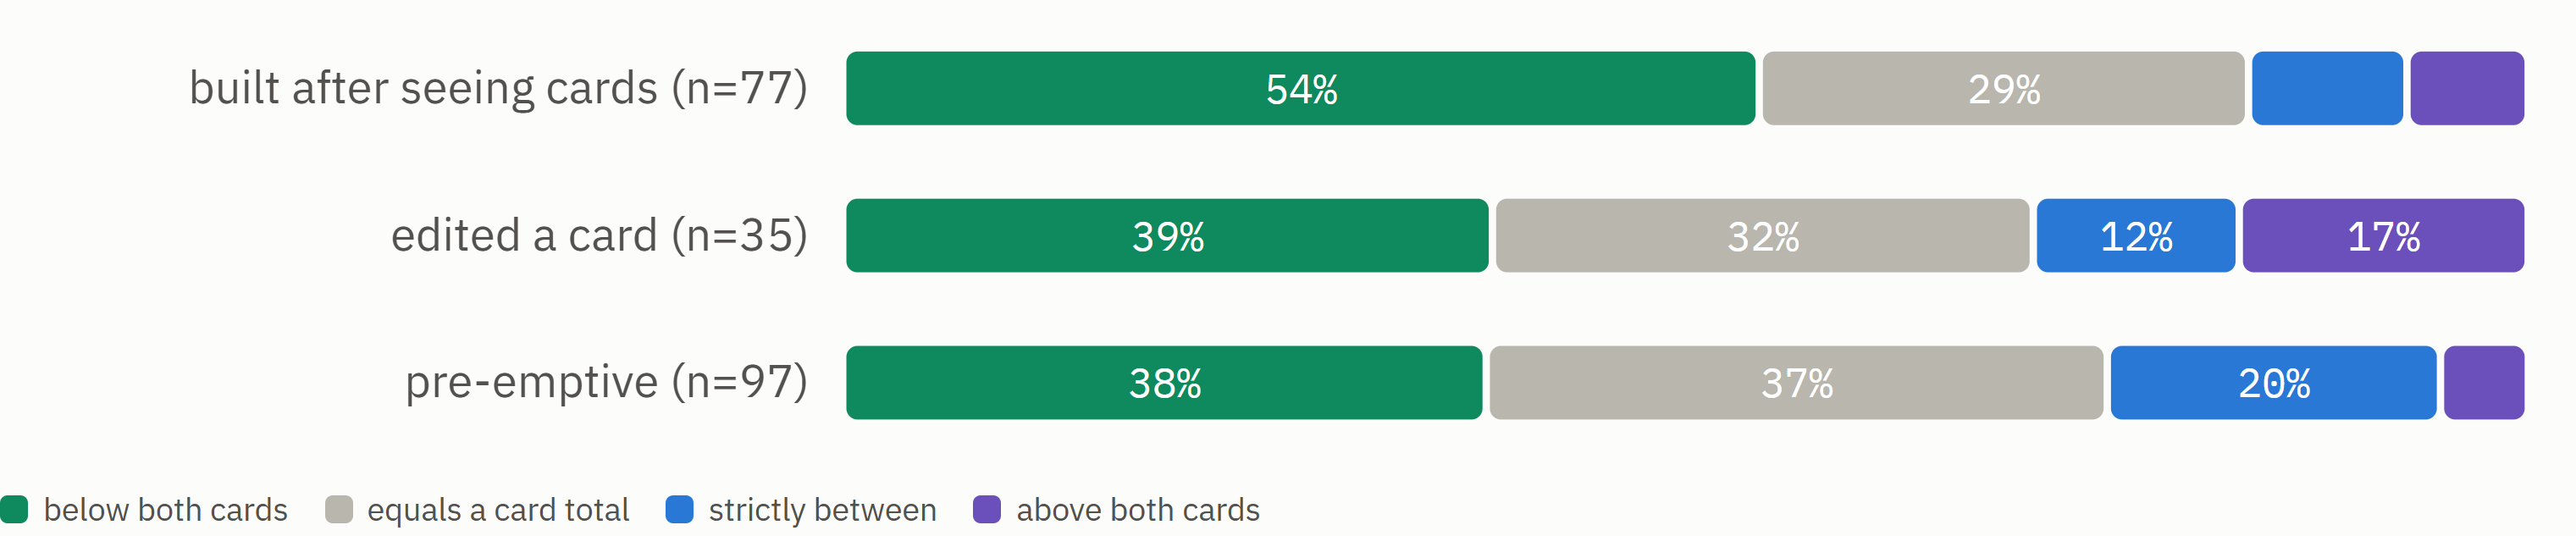
\includegraphics[width=\linewidth,height=0.23\textheight,keepaspectratio]{figs/results/f-manual-cards__position__balanced.png}
\caption{Balanced for mission size, drone types, the gap between the cards, game, session and minute.}
\label{fig:res:manual-cards:position:balanced}
\end{subfigure}
\par\smallskip
\caption{\textbf{Where manual builds sit relative to the two cards}}
\label{fig:res:manual-cards:position}
\end{figure}

\paragraph*{Key numbers.}

\begin{itemize}[leftmargin=1.2em,itemsep=1pt]

\item All 209: below both 44\%, equal to a card 33\%, strictly between 14\%, above both 8\%

\item Built after seeing (77): 57\% below, 27\% equal, 9\% between, 6\% above; pre-emptive (97): 38\%, 39\%, 16\%, 6\%

\item Mission mix: pre-emptive builds needed 6.9 drones on average (after seeing 7.6, edited 9.3) and 52\% were one drone type (38\%, 23\%).

\item Balanced: after seeing 54\% below, 29\% equal, 9\% between, 7\% above; pre-emptive 38\%, 37\%, 20\%, 5\%; edited a card 39\%, 32\%, 12\%, 17\%.

\item Pre-emptive minus after seeing, balanced: equal to a card +8 points [$-$10, +23] (raw +12); below both $-$16 [$-$33, +4] (raw $-$19).

\end{itemize}

\paragraph*{Method.} {\small Each manual total compared with the two card totals (all types): below both, equal to either, strictly between, above both. Counts per kind of manual decision. \textbf{Balanced view}: one logistic model per position (below both / equal / between / above) on the kind of build + drones needed + number of drone types + the gap between the two card totals + game + session + minute. Every one of the 209 builds is predicted as each kind in turn and averaged, so the three kinds are compared on the same mix of missions; the four shares are rescaled to 100\%. Intervals: people resampled 1,000 times, models refitted. The person is not held fixed (too few builds each).}

\paragraph*{What participants said.} \regtext{6 of 33 wanted something between the two cards (C08), and P17 says in play that they aim 'between' them. Most of what people say describes trimming a card or matching it, which fits 'below or equal'. 'Equal to a card' was often their own count arrived at first: P30 and P03 work out a number while the cards load and see whether a card matches, and P32 stopped waiting once the cards matched their count.}

\paragraph*{Quotes selected for this section.}

\begin{quotelist}

\item ``But whenever I clicked manual, it's either been for the cause of 'they are sending too much', or I want it to be somewhere between those two levels.''\,---\,P17 (debrief 0:23:38)

\item ``I felt like sometimes I could find like a middle ground that had like maybe a little bit of gambling in there, essentially, that you wouldn't have the necessary coverage.''\,---\,P22 (debrief 0:28:57)

\end{quotelist}

\clearpage

\subsubsection{What operators say about building by hand}\label{sec:res:manual-cards:said}

\noindent \regtext{Four accounts of manual allocation sit alongside the numbers. Holding drones in reserve (C07, 6 people) fits the 'below both cards' mass --- though in the logs these six are not lower than others on needed types (+0.36 vs the Conservative card). Wanting a middle ground or more options (C08, 6 people) fits the wish, not the behaviour: only 10\% of their manual builds land strictly between the cards. Treating a card as a first draft (C09, 4 people) shows in the logs --- 16 of their 33 manual decisions are edited cards. Testing the assistant against themselves (C10, 5 people) fits slower, deliberate manual builds (round 1: 20 s vs 12.6 s). All four describe manual as working \emph{with} the advice, not rejecting it.}

\paragraph*{Key numbers.}

\begin{itemize}[leftmargin=1.2em,itemsep=1pt]

\item C07: 55 manual decisions from 6 people, mean +0.36 vs Conservative on needed types, 21 edited cards

\item C08: 40 from 5 people, 10\% strictly between the cards

\item C09: 33 from 4 people, 16 edited cards

\item C10: 40 from 5 people

\end{itemize}

\paragraph*{Method.} {\small Codes from docs/analysis/qual/codes\_matrix.csv; per-code manual numbers from the same rows as the dot chart (small groups, descriptive only).}

\paragraph*{What participants said.} \regtext{The four accounts are all present in people's own words. They hold drones back (C07, 6), want a middle ground (C08, 6), treat a card as a draft (C09, 4: 'you can fix bad, you can't fix nothing') and test themselves against the assistant (C10, 5). The think-aloud shows the draft habit more widely than coded: P10, P14 and P31 edit cards, and P21 and P31 use Suggest as a first draft on the tactical tier. The one person who tested themself said it ended in favour of the assistant (P29).}

\clearpage

\subsection{Practice makes operators faster, not better at choosing when to hand over}\label{sec:res:practice}

\regtext{\textbf{Summary.} Decisions speed up within each session: about 6\% faster per minute on both tiers, and not because the queue gets longer. On the strategic tier most of that gain is gone by the start of the next session (median 11.6 s at the start of session 1, 6.9 s at its end, 10.6 s at the start of session 2), so it reads as a within-session warm-up more than durable learning. On the tactical tier session 2 starts about where session 1 ended. The size rule does not sharpen with practice: the big-minus-small hand-over gap is the same or smaller in session 2. The six people who say they got better did improve their scores (all six, against 37\% of others), but they did not come to use the assistants more, and across everyone a bigger score gain does not go with more use.} \par\noindent{\small\textit{Strength of evidence (register rating): moderate. Your verdict: keep.}}

\subsubsection{Faster within a session; on the strategic tier the gain mostly resets by the next}\label{sec:res:practice:speed}

\noindent \passtag{numbers only}

\noindent \regtext{Median net decision time through each session, by pair of minutes. On the strategic tier decisions get much faster through a session (11.6 $\rightarrow$ 6.9 s in session 1) and then start nearly as slow again (10.6 s), before speeding up once more (5.8 s). The model keeps about half of the gain across the break, but uncertainly. On the tactical tier the first session's speed-up is weaker and session 2 starts about where session 1 ended, then speeds up again. Holding the number of waiting missions fixed does not remove the within-session speed-up, so it is not just time pressure from a longer queue.} (Figure~\ref{fig:res:practice:speed})

\begin{figure}[H]
\centering
\begin{subfigure}[t]{0.495\linewidth}
\centering
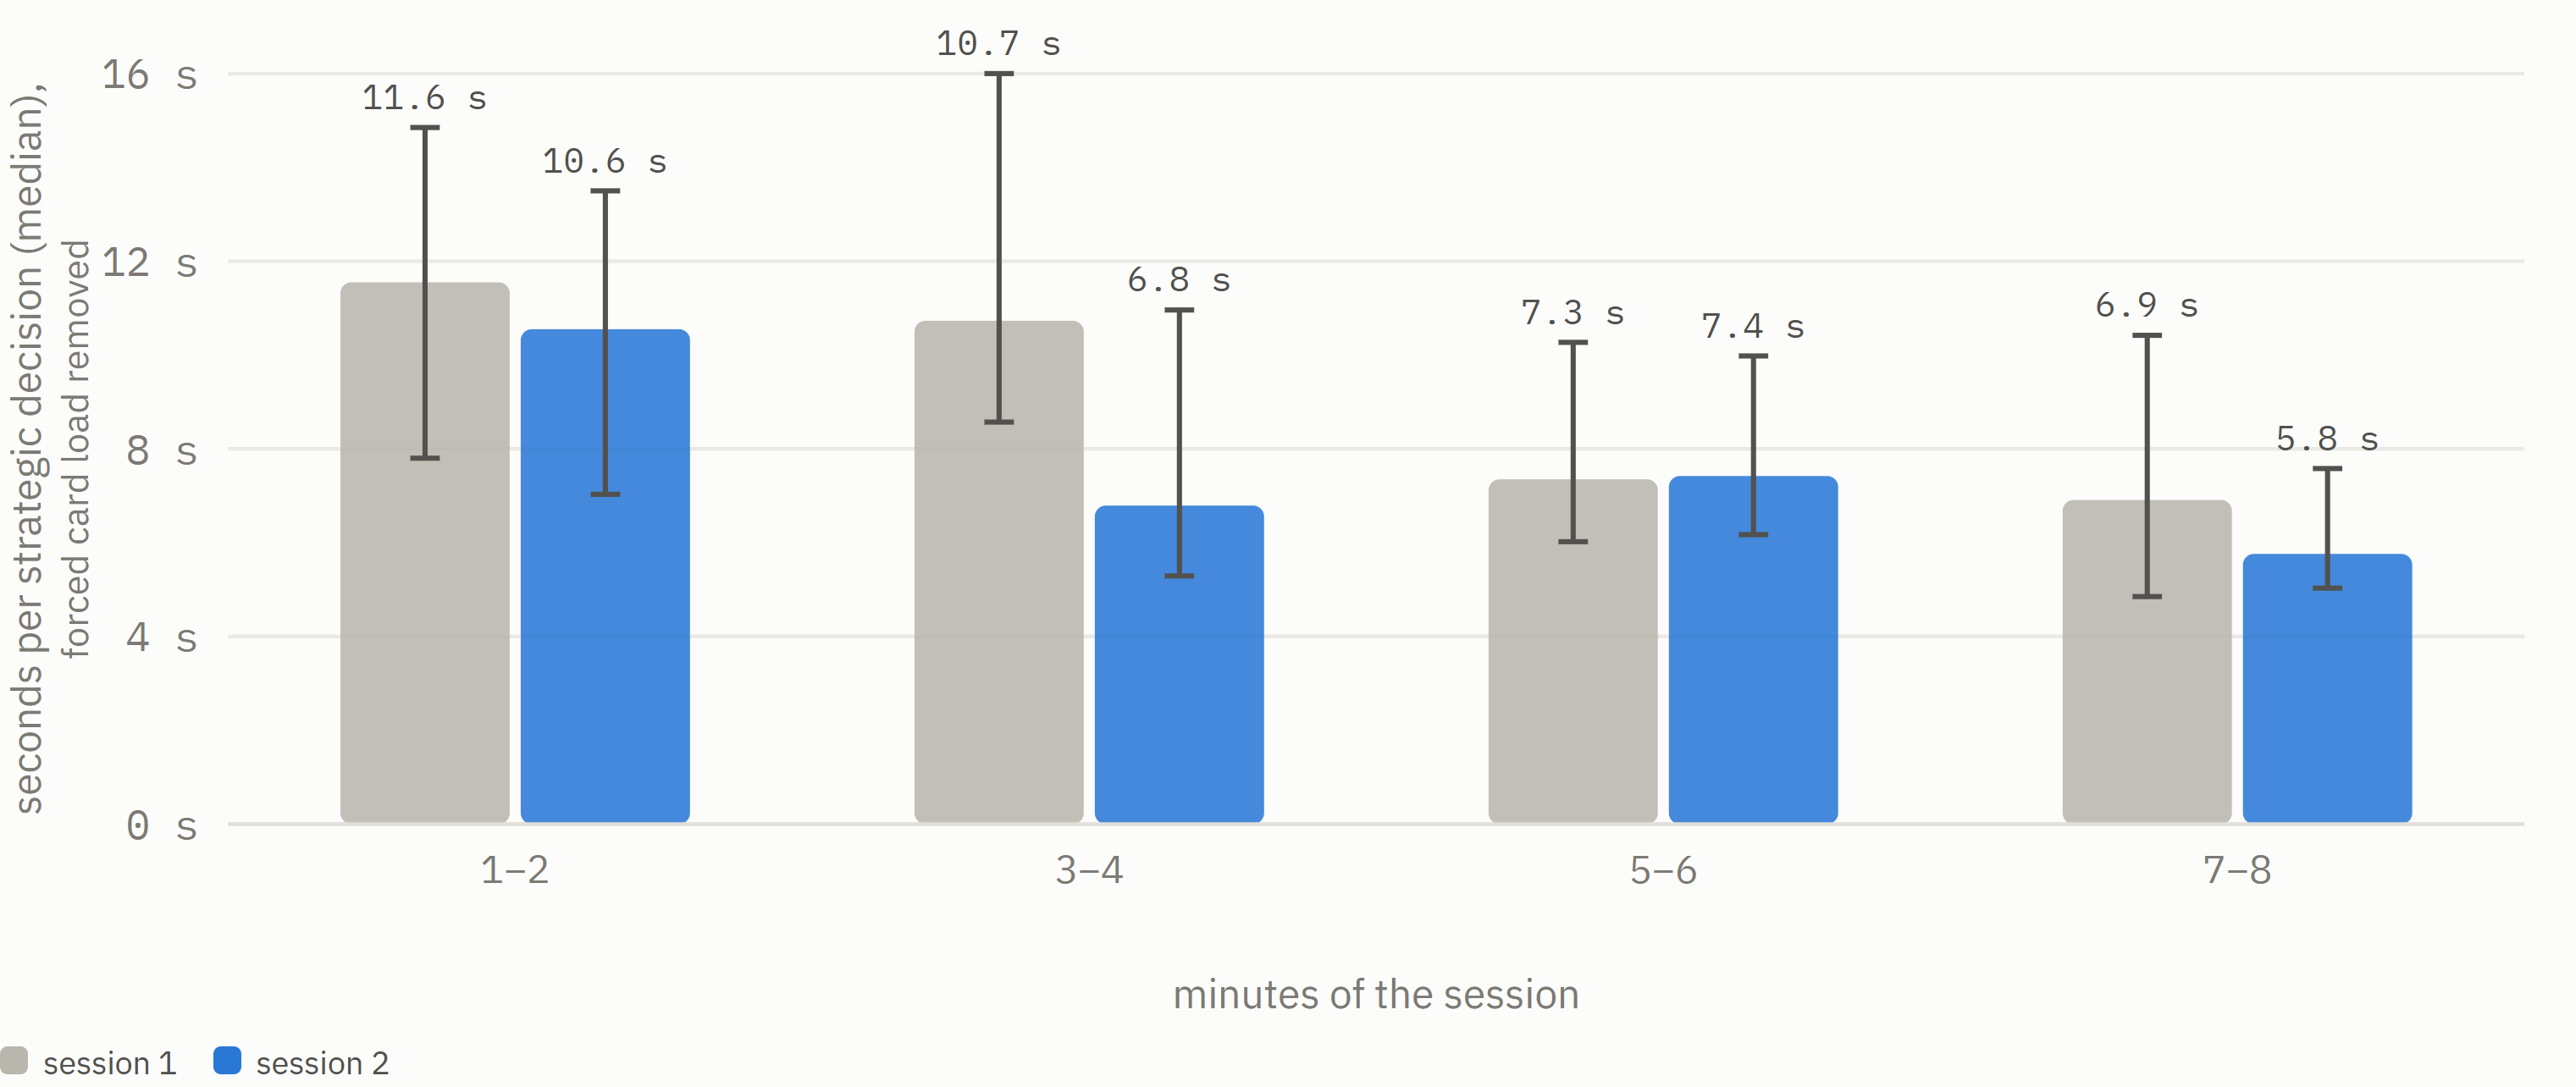
\includegraphics[width=\linewidth,height=0.23\textheight,keepaspectratio]{figs/results/f-practice__speed__strat.png}
\caption{Strategic tier, sessions side by side.}
\label{fig:res:practice:speed:strat}
\end{subfigure}
\hfill
\begin{subfigure}[t]{0.495\linewidth}
\centering
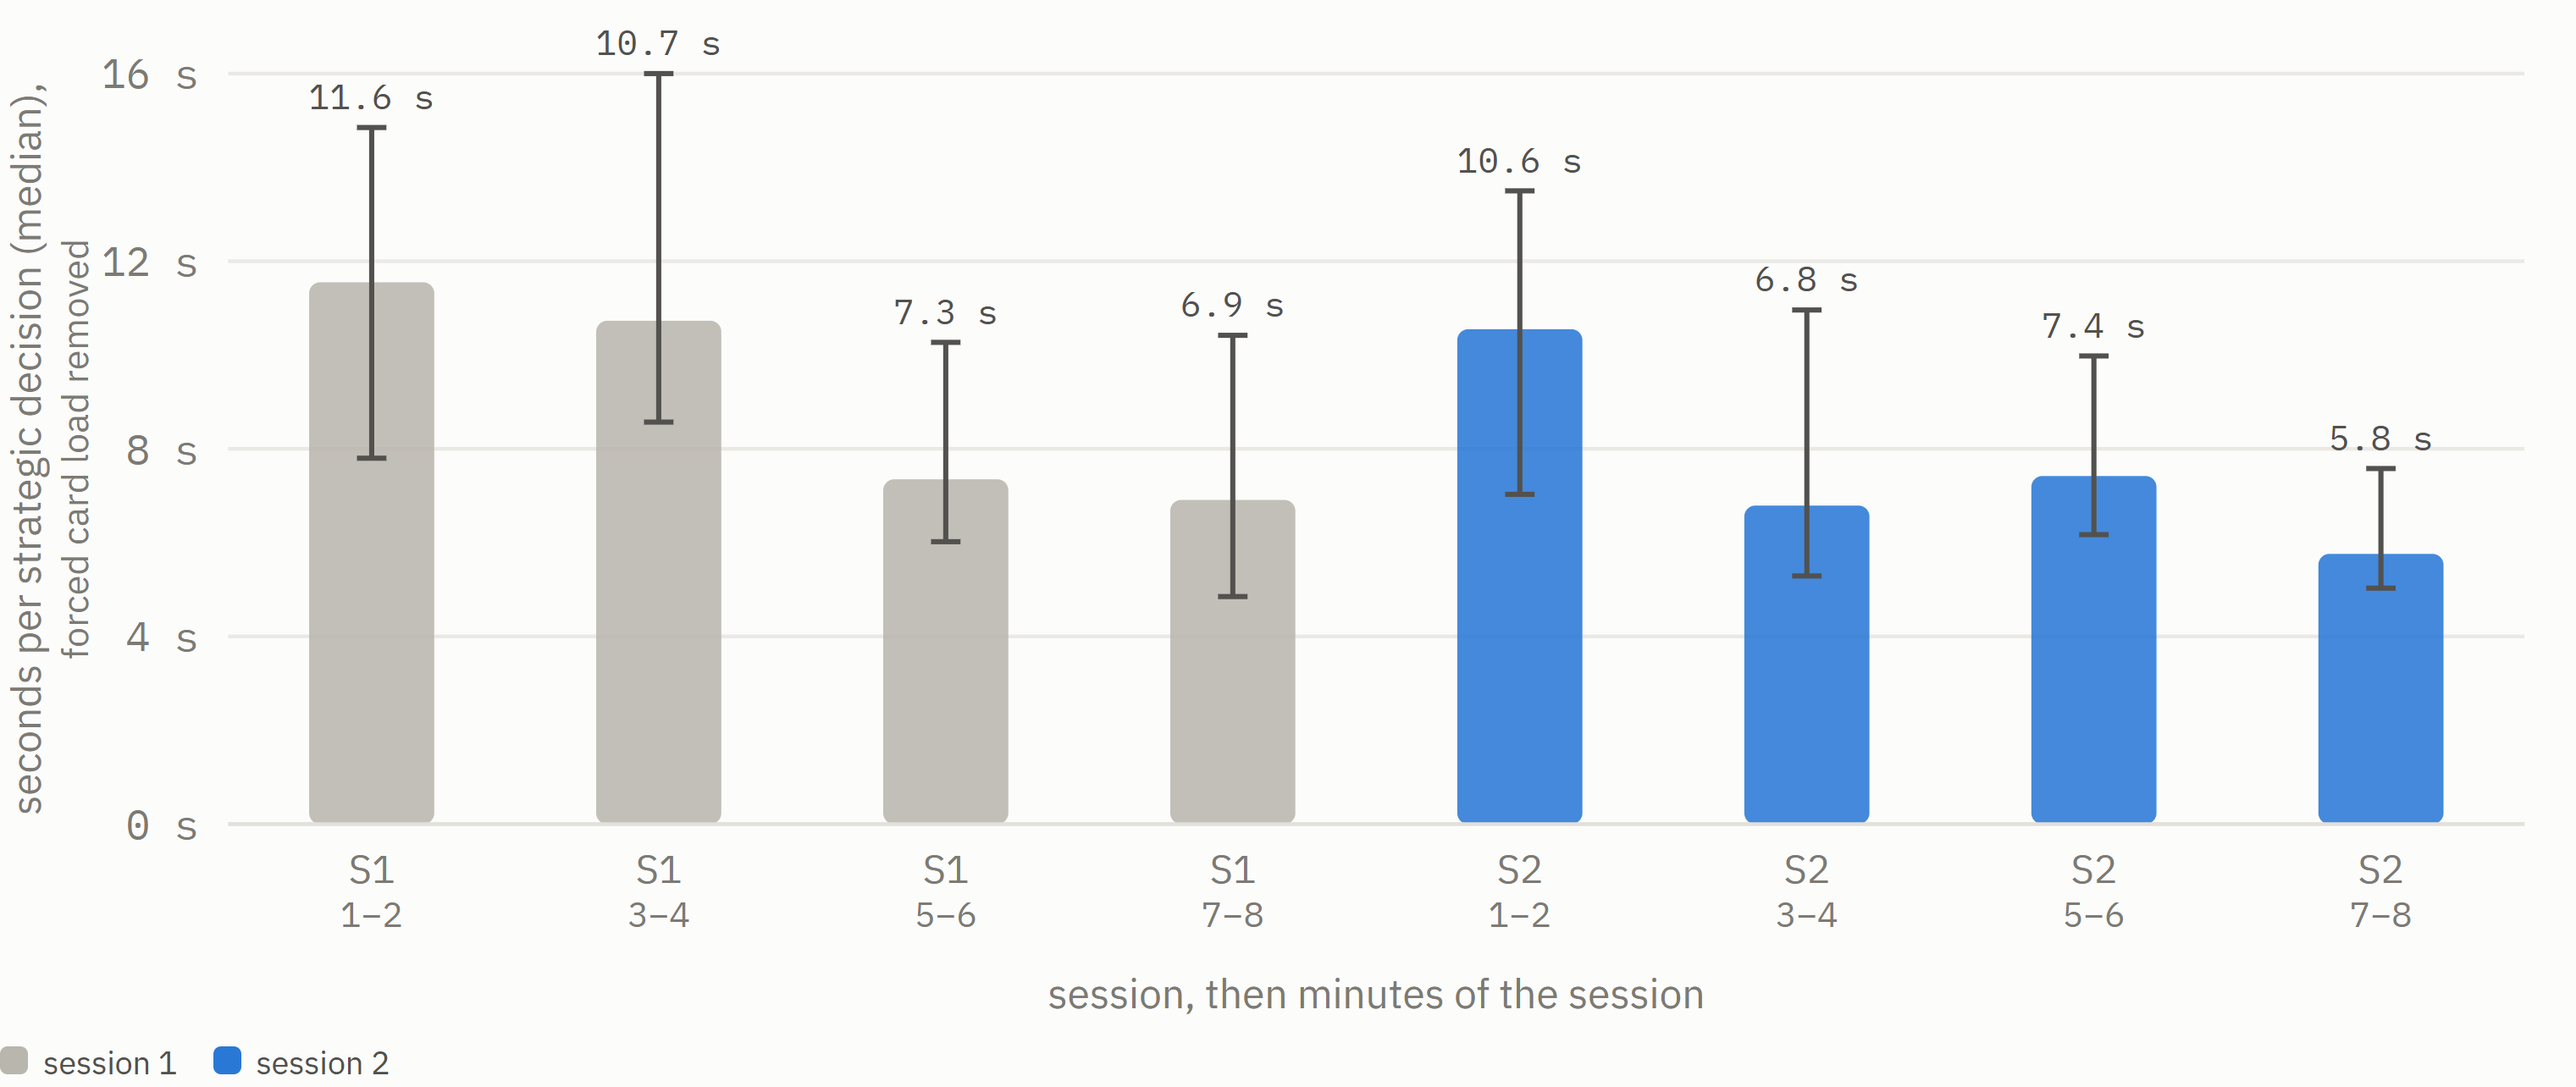
\includegraphics[width=\linewidth,height=0.23\textheight,keepaspectratio]{figs/results/f-practice__speed__strat-order.png}
\caption{Strategic tier, all of session 1 then all of session 2.}
\label{fig:res:practice:speed:strat-order}
\end{subfigure}
\par\smallskip
\begin{subfigure}[t]{0.495\linewidth}
\centering
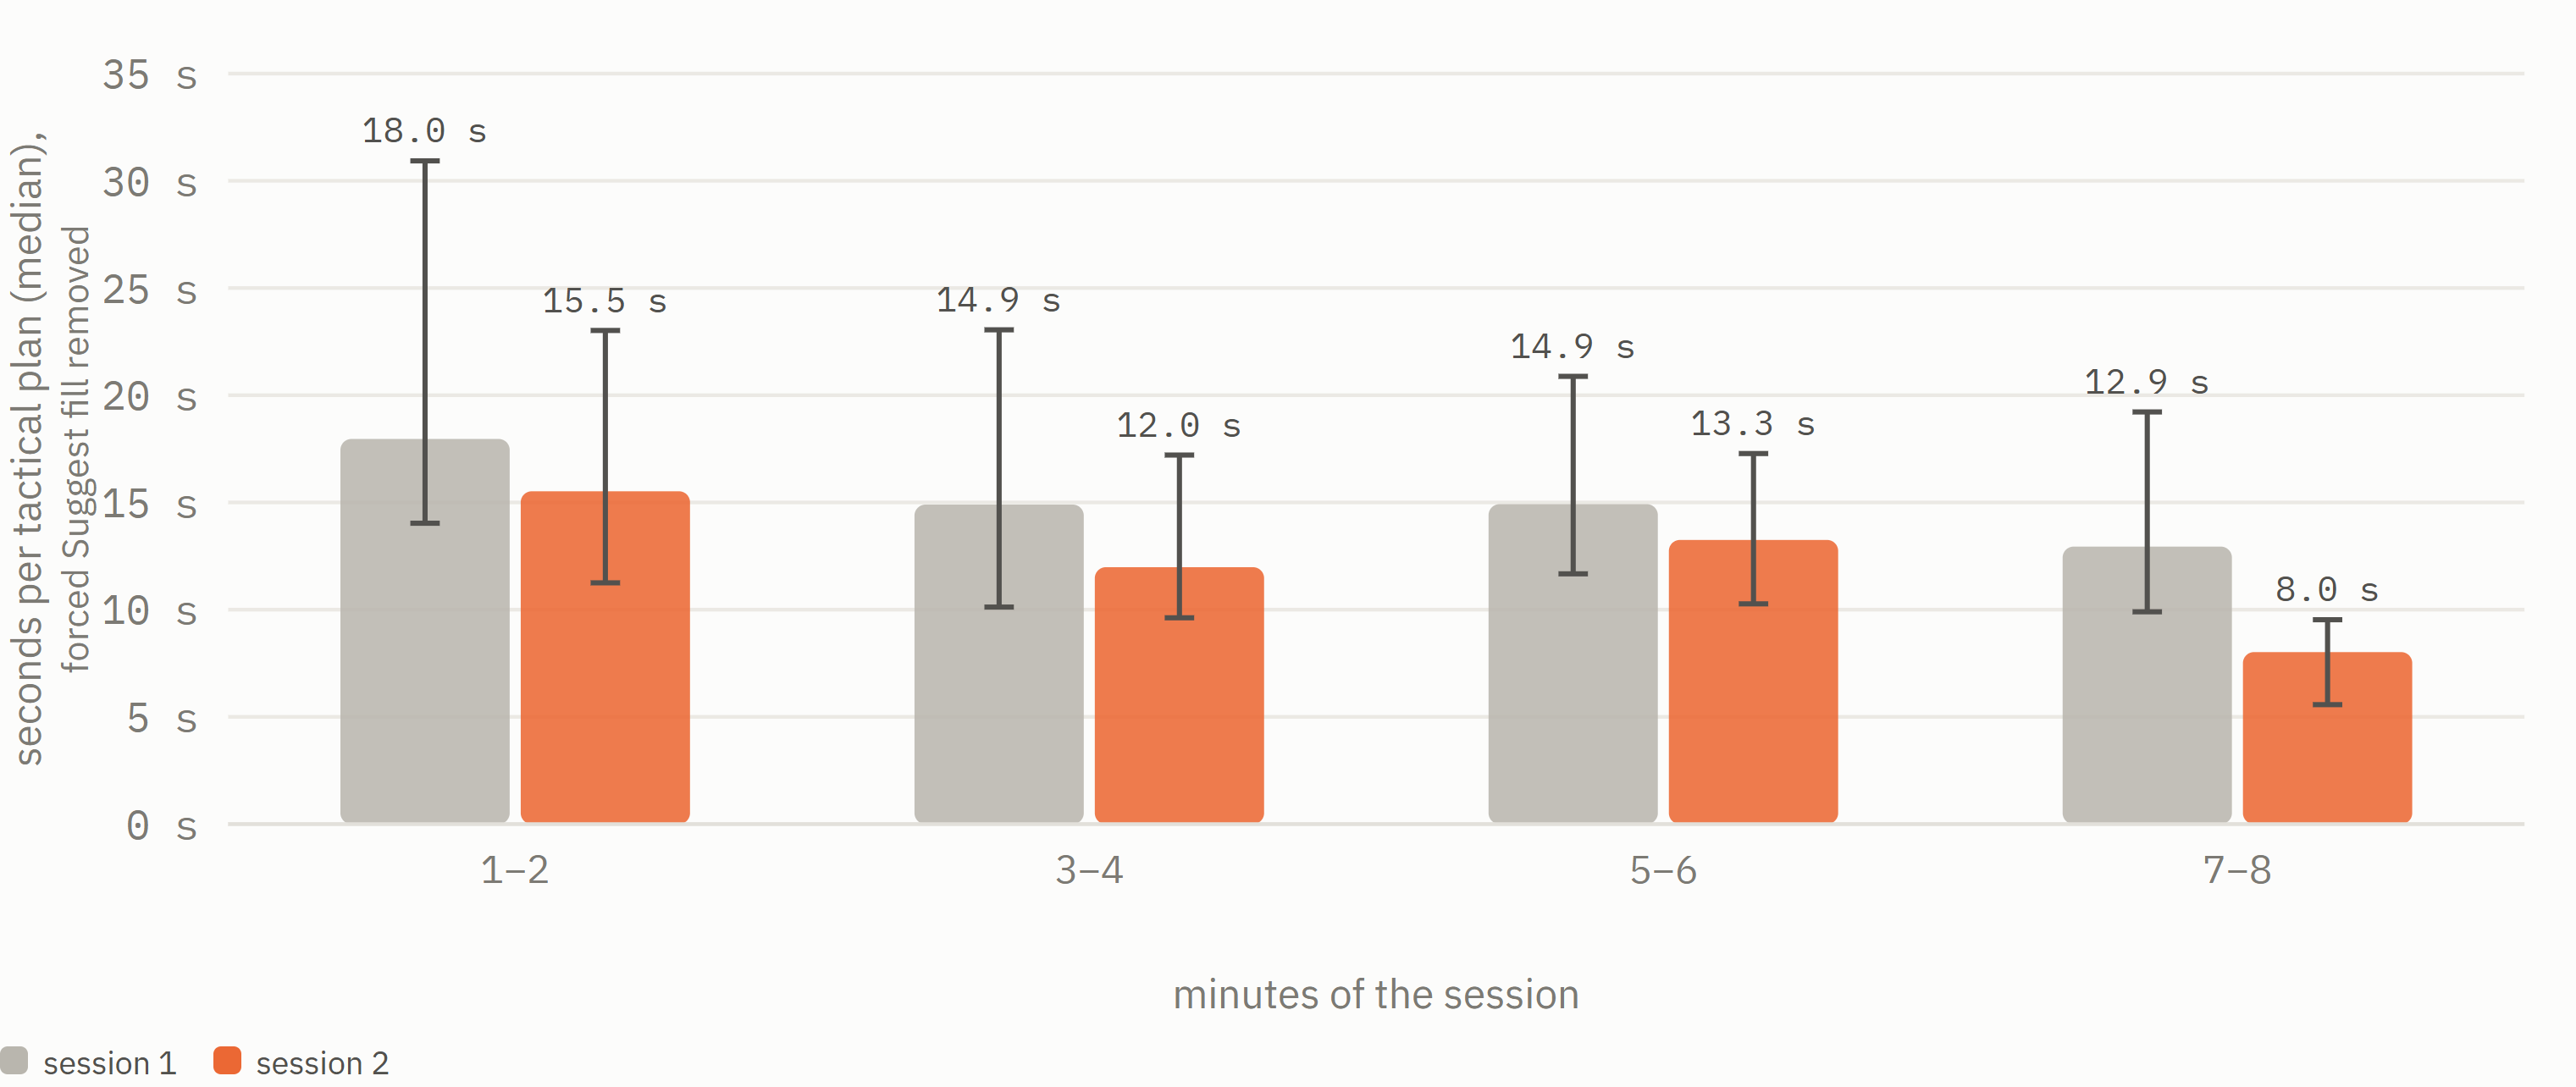
\includegraphics[width=\linewidth,height=0.23\textheight,keepaspectratio]{figs/results/f-practice__speed__tac.png}
\caption{Tactical tier, sessions side by side.}
\label{fig:res:practice:speed:tac}
\end{subfigure}
\hfill
\caption{\textbf{Faster within a session; on the strategic tier the gain mostly resets by the next}}
\label{fig:res:practice:speed}
\end{figure}

\paragraph*{Key numbers.}

\begin{itemize}[leftmargin=1.2em,itemsep=1pt]

\item Strategic, medians: session 1 minutes 1--2 11.6 s [7.8, 14.5] $\rightarrow$ minutes 7--8 6.9 s [4.9, 10.2]; session 2 10.6 s [7.0, 13.5] $\rightarrow$ 5.8 s [5.0, 7.6]

\item Strategic, model: end of session 1 $-$39\% [$-$51, $-$24]; start of session 2 $-$20\% [$-$37, +2], p = .07; start of session 2 vs end of session 1 +31\% [0, +72], p = .053 (slower again)

\item Tactical, medians: 18.0 s [14.0, 30.9] $\rightarrow$ 12.9 s [10.1, 19.2]; session 2 15.5 s [11.3, 21.9] $\rightarrow$ 8.0 s [5.6, 9.6]

\item Tactical, model: end of session 1 $-$24\% [$-$45, +4], p = .09; start of session 2 vs end of session 1 +2\% [$-$33, +56], p = .92; session 2 slope $-$7\% per minute vs $-$4\% in session 1 (difference p = .26)

\item Within-session slope with the queue held fixed: strategic $-$6\% per minute, tactical $-$8\% per minute (both p < .001)

\item Overall (unchanged): strategic $-$5.7\% per minute [$-$7.8, $-$3.6], session 2 vs 1 $-$19\% [$-$30, $-$6]; tactical $-$5.7\% per minute [$-$9.1, $-$2.2], session 2 vs 1 $-$24\% [$-$36, $-$9]

\end{itemize}

\paragraph*{Method.} {\small \textbf{Net time} = seconds to decide minus the forced wait (the card reveal for card choices; 1 s per entry for Suggest plans). Bars: medians of all decisions made in minutes 1--2 and 7--8 of each session, with 95\% intervals from resampling people. \textbf{Model}: Gaussian GEE on log net time, clustered on person, with minute of session, session 2 and their interaction, plus route and mission size; game held fixed. From it: the end of session 1, and the start and end of session 2, each relative to the start of session 1, and the start of session 2 relative to the end of session 1 (a positive value = slower again after the break). A log-scale coefficient converts to ``\% faster''. The start of a session is also the start of a game (first missions, short queue), so part of a within-session speed-up may be the session's own rhythm rather than learning.}

\paragraph*{What participants said.} \regtext{People describe getting faster and finding their rhythm: P10 'find your stride', P30 'got into the rhythm', P35 'getting familiar', P11 'get the hang of it quite quickly'. Several state a lesson from session 1 at the start of session 2: P22 'don't send everything straight away', P06 'the task will get a lot pretty quickly'. P18 is a partial dissent: the second session felt better prepared but more stressful.}

\paragraph*{Quotes selected for this section.}

\begin{quotelist}

\item ``there was definitely an improvement further throughout session one, and in session two, you really find your stride''\,---\,P10 (debrief 0:22:57)

\item ``i think the second scenario i used more personalised, i think it was easier because i had to i sort of got into the rhythm of having to anticipate other problems''\,---\,P30 (debrief 0:23:52)

\item ``Right. So now we also know from the last one, don't send everything straight away. Cause otherwise we end up, we're waiting for drones.''\,---\,P22 (think-aloud s2 0:17:11)

\item ``And I could definitely feel that there is absolutely a learning effect.''\,---\,P10 (debrief 0:22:39)

\item ``I think with having some experience, yeah, I was able to quickly understand this''\,---\,P05 (think-aloud s1 0:11:14)

\end{quotelist}

\clearpage

\subsubsection{Does 'I got better with practice' match the logs? For score yes; not for speed or assistant use}\label{sec:res:practice:c22}

\noindent \passtag{numbers only}

\noindent \regtext{Six people say they got better, faster or more confident (C22: P10, P11, P15, P21, P30, P32). All six raised their within-game score from session 1 to 2, against 10 of 27 others. Their tactical planning sped up more than others' on average (5 of 6 faster), but not reliably; their strategic decisions did not speed up more. They also \textbf{did not come to use the assistants more}: strategy cards taken changed by $-$1 point (others $-$4) and Suggest by +11 points (others +7), with 3 of the 6 using each assistant more in session 2. Across all 33 people, a bigger score gain does not go with a bigger rise in either kind of use. So ``got better'' is right about outcomes, but it is not ``relied on the assistants more''.} (Figure~\ref{fig:res:practice:c22})

\begin{figure}[H]
\centering
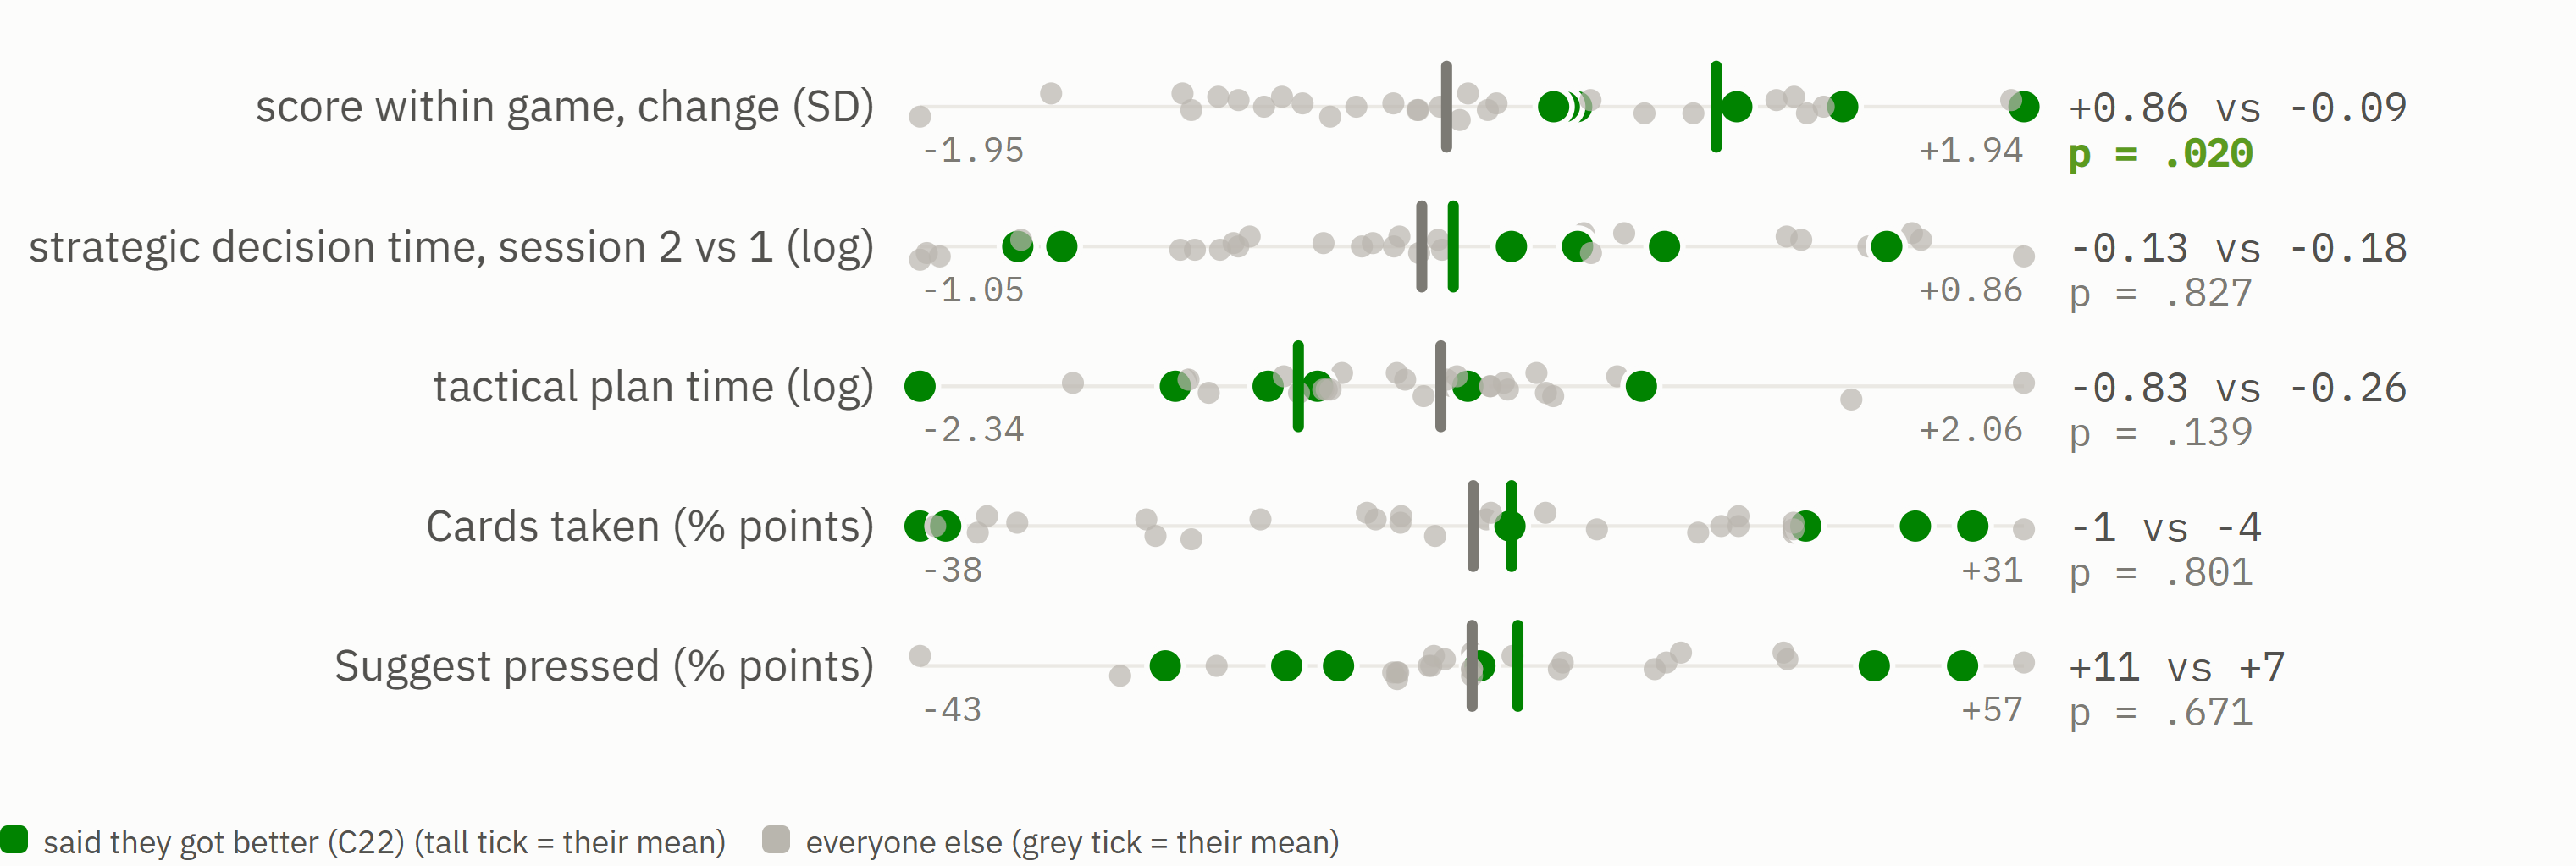
\includegraphics[width=\linewidth,height=0.55\textheight,keepaspectratio]{figs/results/f-practice__c22__main.png}
\caption{\textbf{Does 'I got better with practice' match the logs? For score yes; not for speed or assistant use}}
\label{fig:res:practice:c22}
\end{figure}

\paragraph*{Key numbers.}

\begin{itemize}[leftmargin=1.2em,itemsep=1pt]

\item Score change: C22 +0.86 SD vs others $-$0.09, p = .020

\item Tactical time change (log): $-$0.83 vs $-$0.26, p = .14; strategic: $-$0.13 vs $-$0.18, p = .83

\item Change in cards taken (game-adjusted): C22 $-$1 point vs others $-$4, p = .80; Suggest pressed: +11 vs +7 points, p = .67

\item Used more in session 2: cards 3 of 6 C22 vs 12 of 27 others; Suggest 3 of 6 vs 19 of 27

\item Everyone: score change vs change in card-taking $\rho$ = $-$.07 (p = .71); vs change in Suggest $\rho$ = $-$.18 (p = .32)

\end{itemize}

\paragraph*{Method.} {\small Per person: session 2 minus session 1 in (a) score standardised within game, (b) log median net strategic time, (c) log median net tactical time, (d) share of strategy cards taken and (e) share of plans with Suggest pressed. For (d) and (e) each session's rate is first taken relative to that game's average rate across everyone, so playing a different game in session 2 does not count as a change of habit (raw changes agree). Group mean vs the other 27, two-sided permutation p (20,000 reshuffles). The across-everyone check is a Spearman rank correlation between score change and change in use (33 people). With P01/P02 left out of the game means, P21's score change is slightly negative (five of six, not six).}

\paragraph*{What participants said.} \regtext{6 of 33 say they got better (C22). Their reasons are understanding the task (P32), experience (P11, P15) and optimising how they worked with the assistants (P21), not leaning on the assistants more. Others outside C22 describe practice changing how much they use the assistants, in both directions. P06 and P31 relied more and checked less, P28 expected to rely less once familiar, and P35 used the cards less after spotting errors. That mixed picture fits the logs: no overall rise in use with practice.}

\clearpage

\subsection{A busier moment does not push people onto the assistants --- even though they say it does}\label{sec:res:workload}

\regtext{\textbf{Summary.} Comparing each operator with themselves, having more missions waiting does not change how often they take a strategy card or press Suggest: the line is flat once we account for what each decision was (mission size and drone types), when it came in the session, which game it was and who made it. This is ``no evidence of an effect'', with enough data to rule out large effects (strategic: at most about +15 points of card-taking going from 0 to 5 waiting). Nine of 33 said in the debrief that they hand over when overloaded; their own behaviour moved with the queue no more than anyone else's. In play they said overload-type things at slightly busier moments, but their reliance around those moments did not change.} \par\noindent{\small\textit{Strength of evidence (register rating): a null result. Your verdict: core.}}

\subsubsection{Queue depth against reliance --- raw, and adjusted}\label{sec:res:workload:raw-vs-adjusted}

\noindent \passtag{for the paper}

\noindent \regtext{Each point is the share of decisions where the operator took a strategy card (or pressed Suggest), grouped by how many OTHER missions were waiting for a strategic decision at that moment. Whiskers are 95\% intervals. The dotted vertical line marks where the queue list runs out of room (about 3.5 cards visible at rest, counting the one being opened): beyond it, waiting missions are only on the strategic map. Nothing changes at that line either.} (Figure~\ref{fig:res:workload:raw-vs-adjusted})

\begin{figure}[H]
\centering
\begin{subfigure}[t]{0.495\linewidth}
\centering
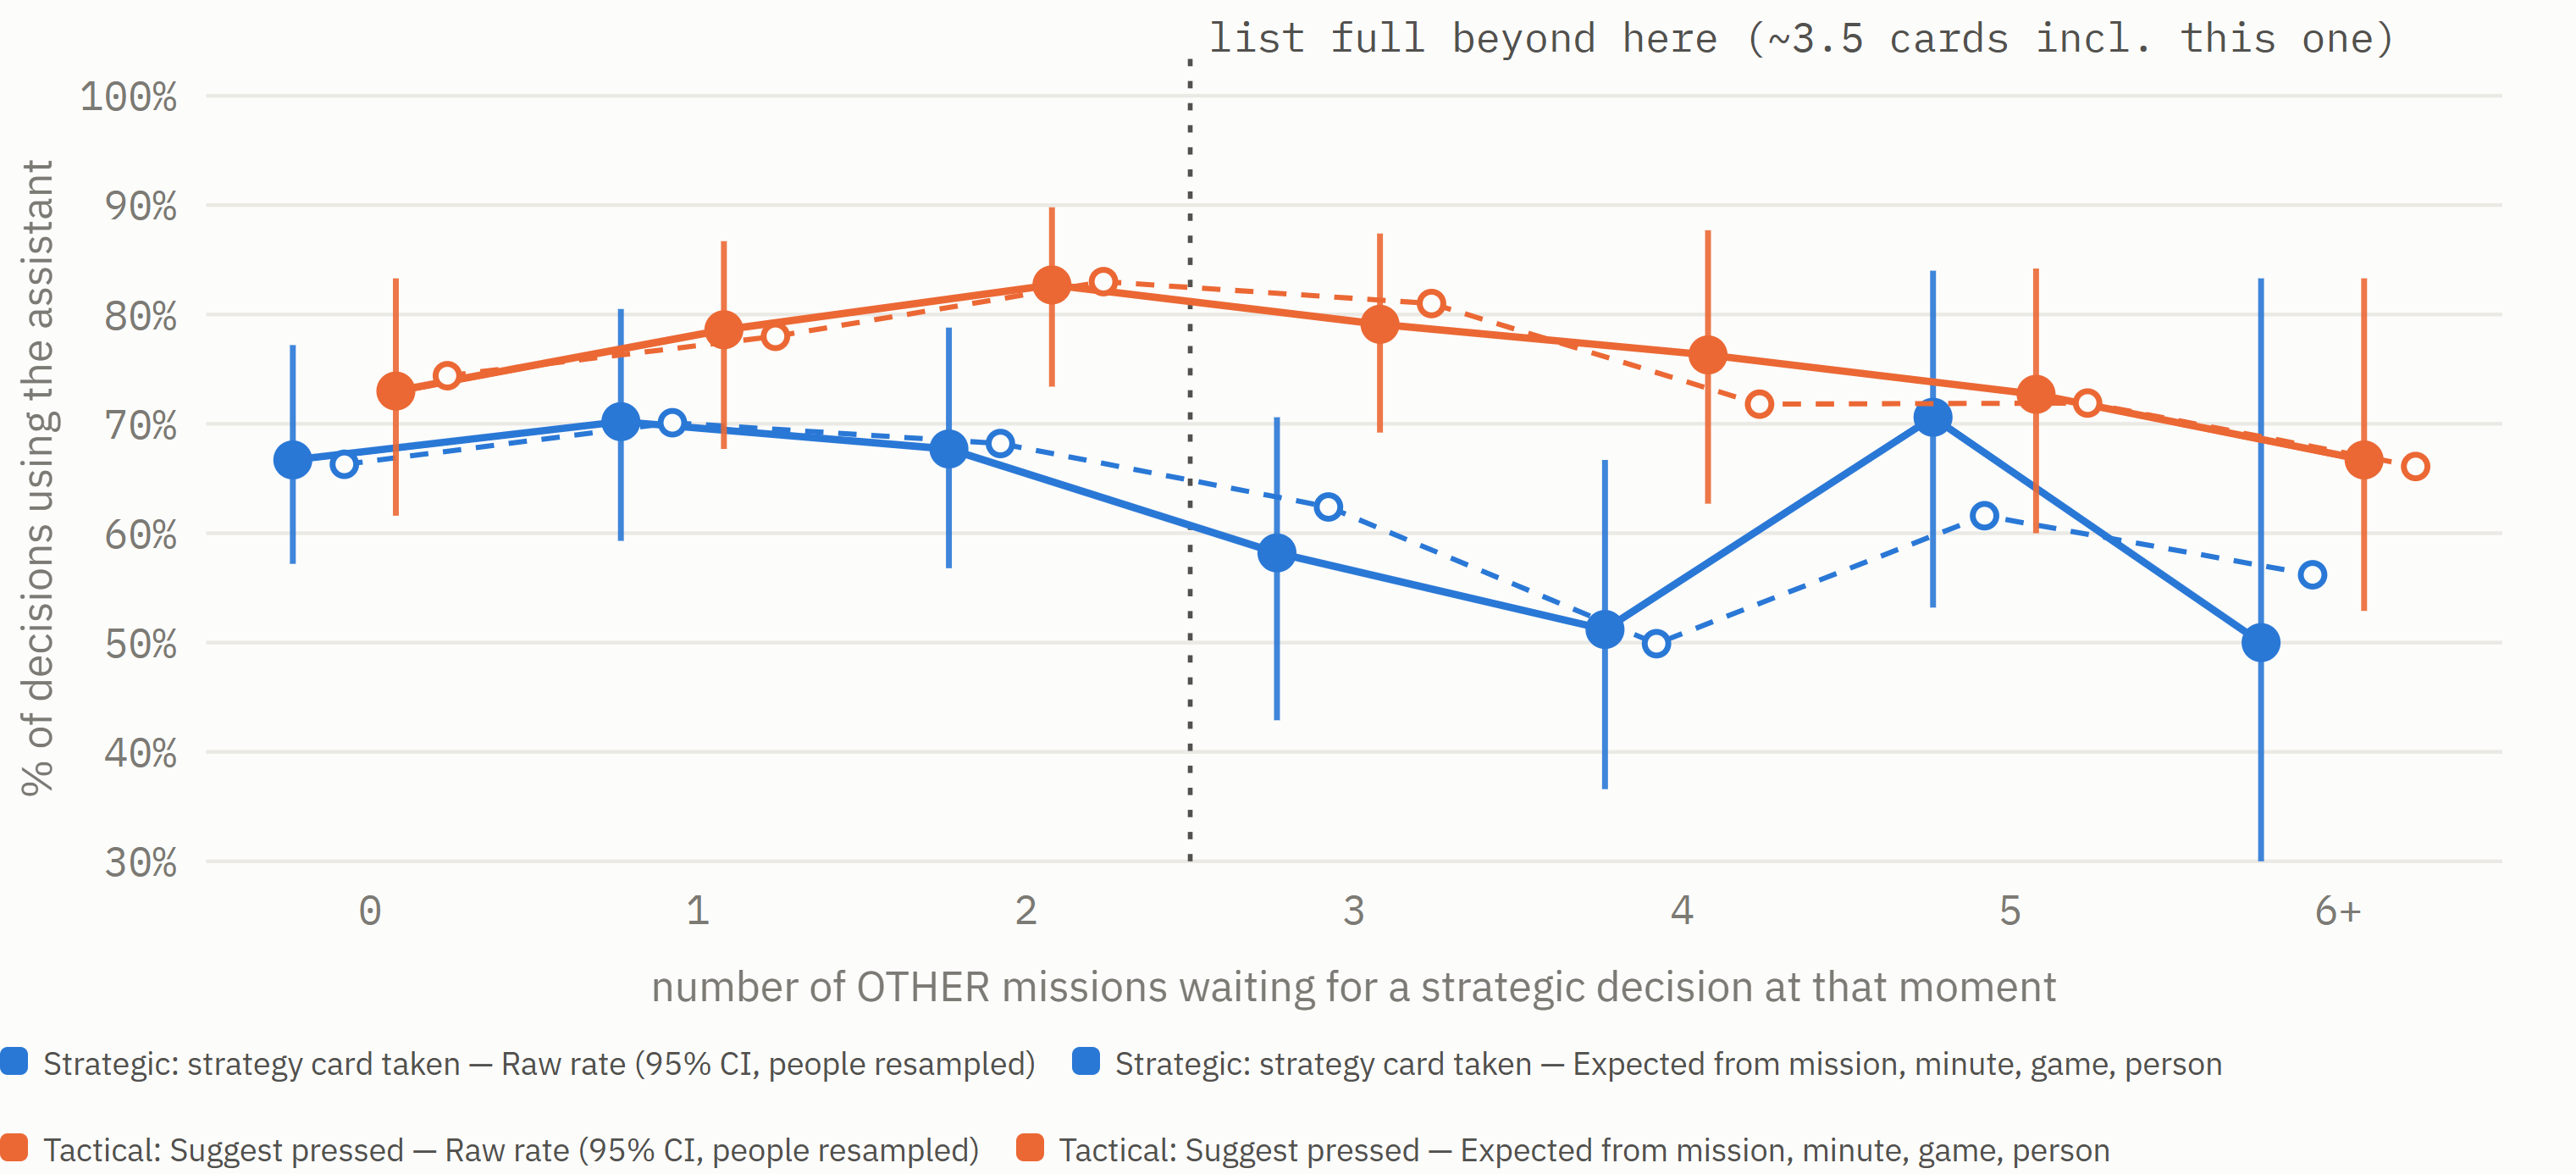
\includegraphics[width=\linewidth,height=0.23\textheight,keepaspectratio]{figs/results/f-workload__raw-vs-adjusted__both-exp.png}
\caption{Both tiers together, raw with their expected rates (dashed).}
\label{fig:res:workload:raw-vs-adjusted:both-exp}
\end{subfigure}
\hfill
\begin{subfigure}[t]{0.495\linewidth}
\centering
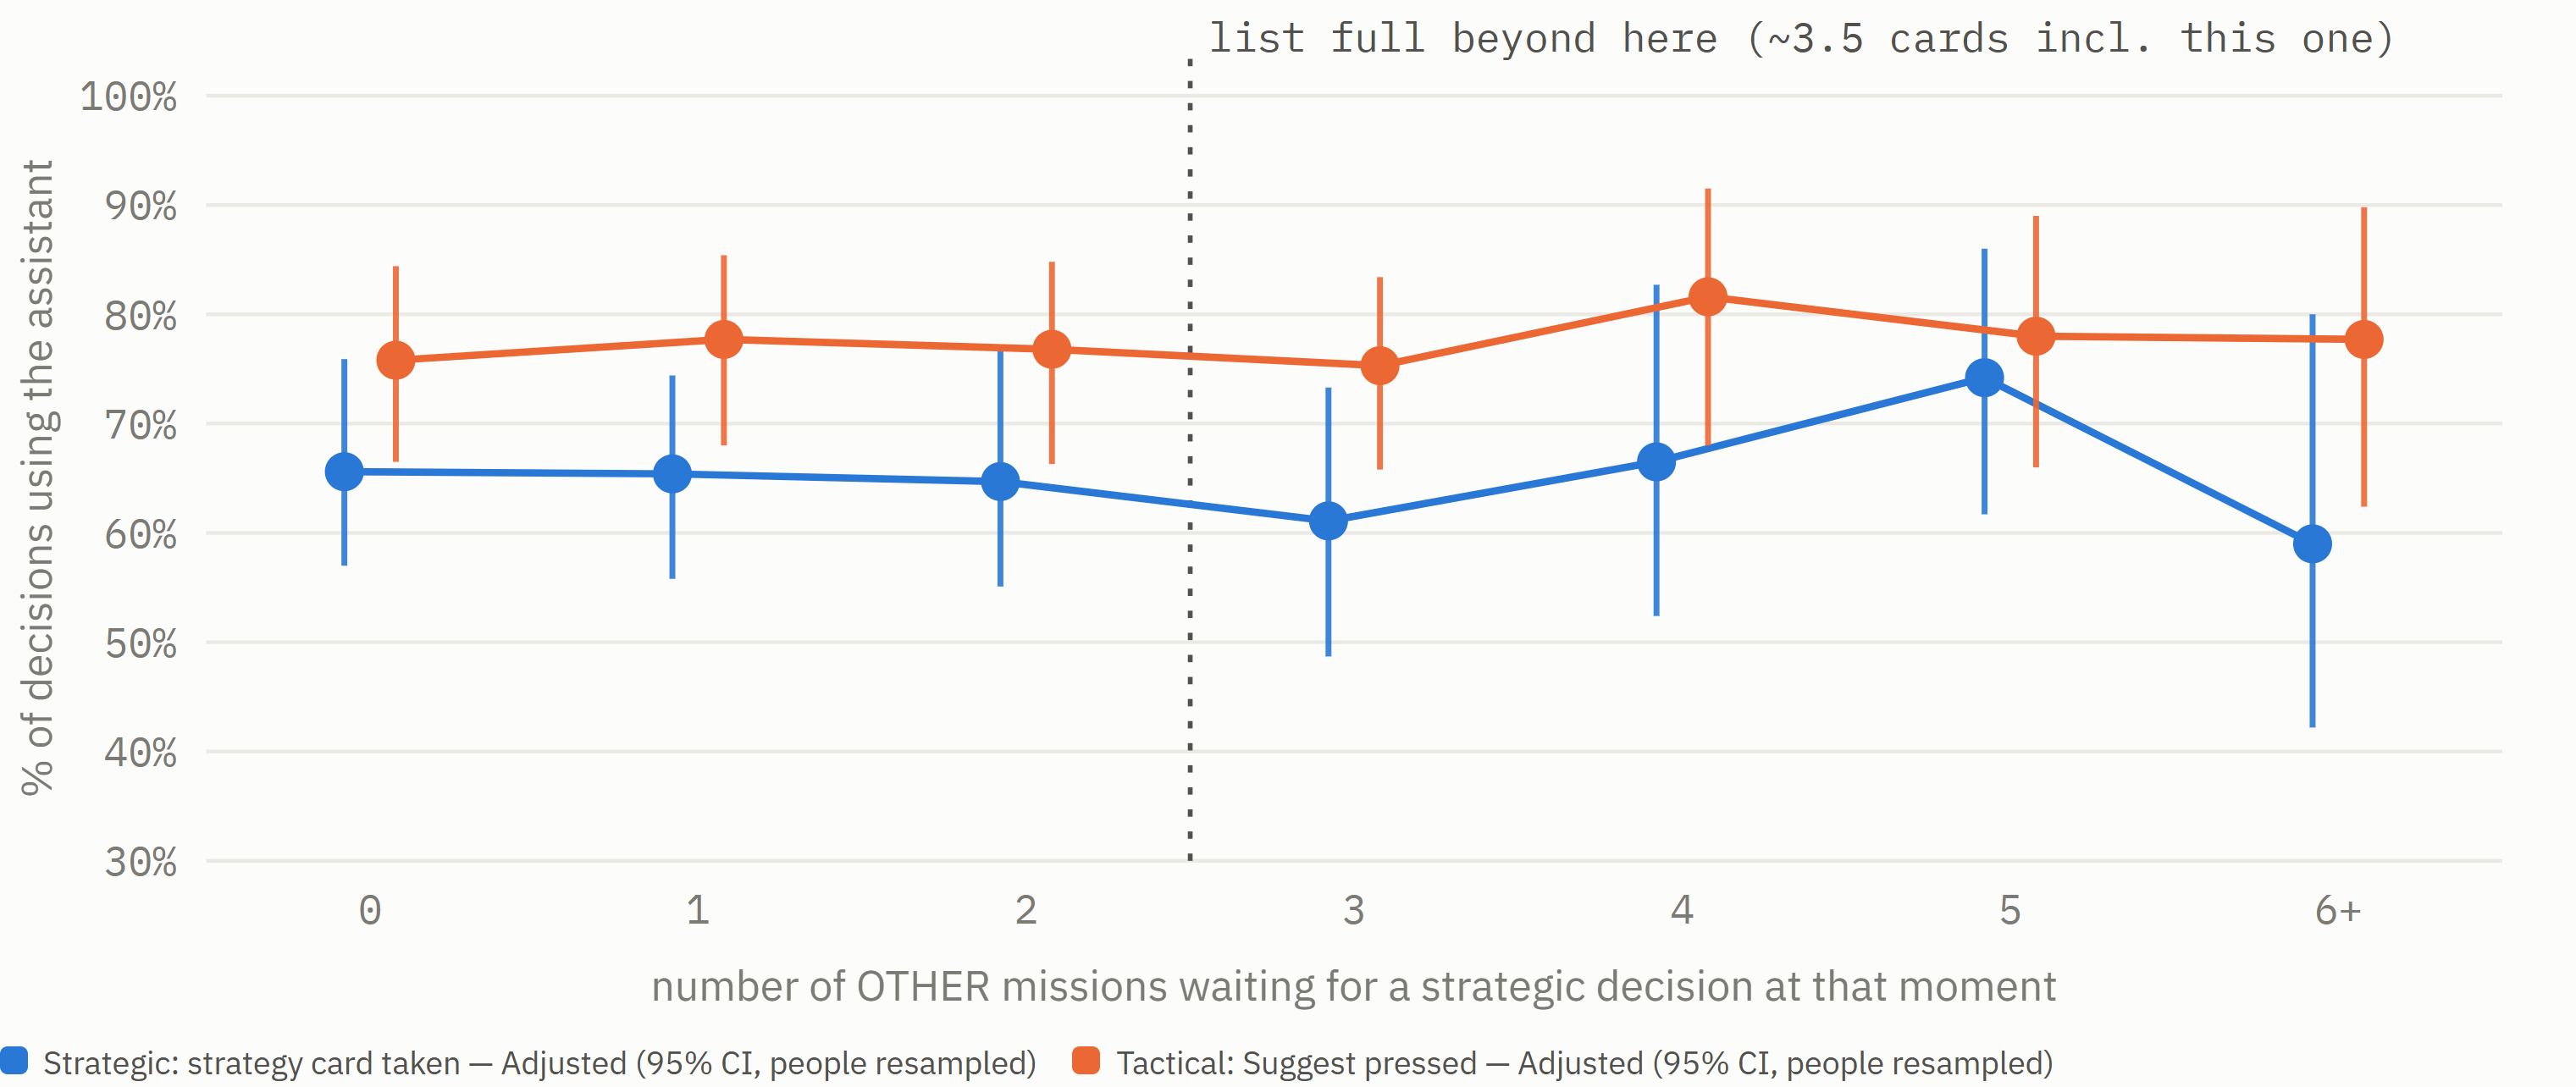
\includegraphics[width=\linewidth,height=0.23\textheight,keepaspectratio]{figs/results/f-workload__raw-vs-adjusted__both-adj.png}
\caption{Both tiers together, adjusted.}
\label{fig:res:workload:raw-vs-adjusted:both-adj}
\end{subfigure}
\par\smallskip
\begin{subfigure}[t]{0.495\linewidth}
\centering
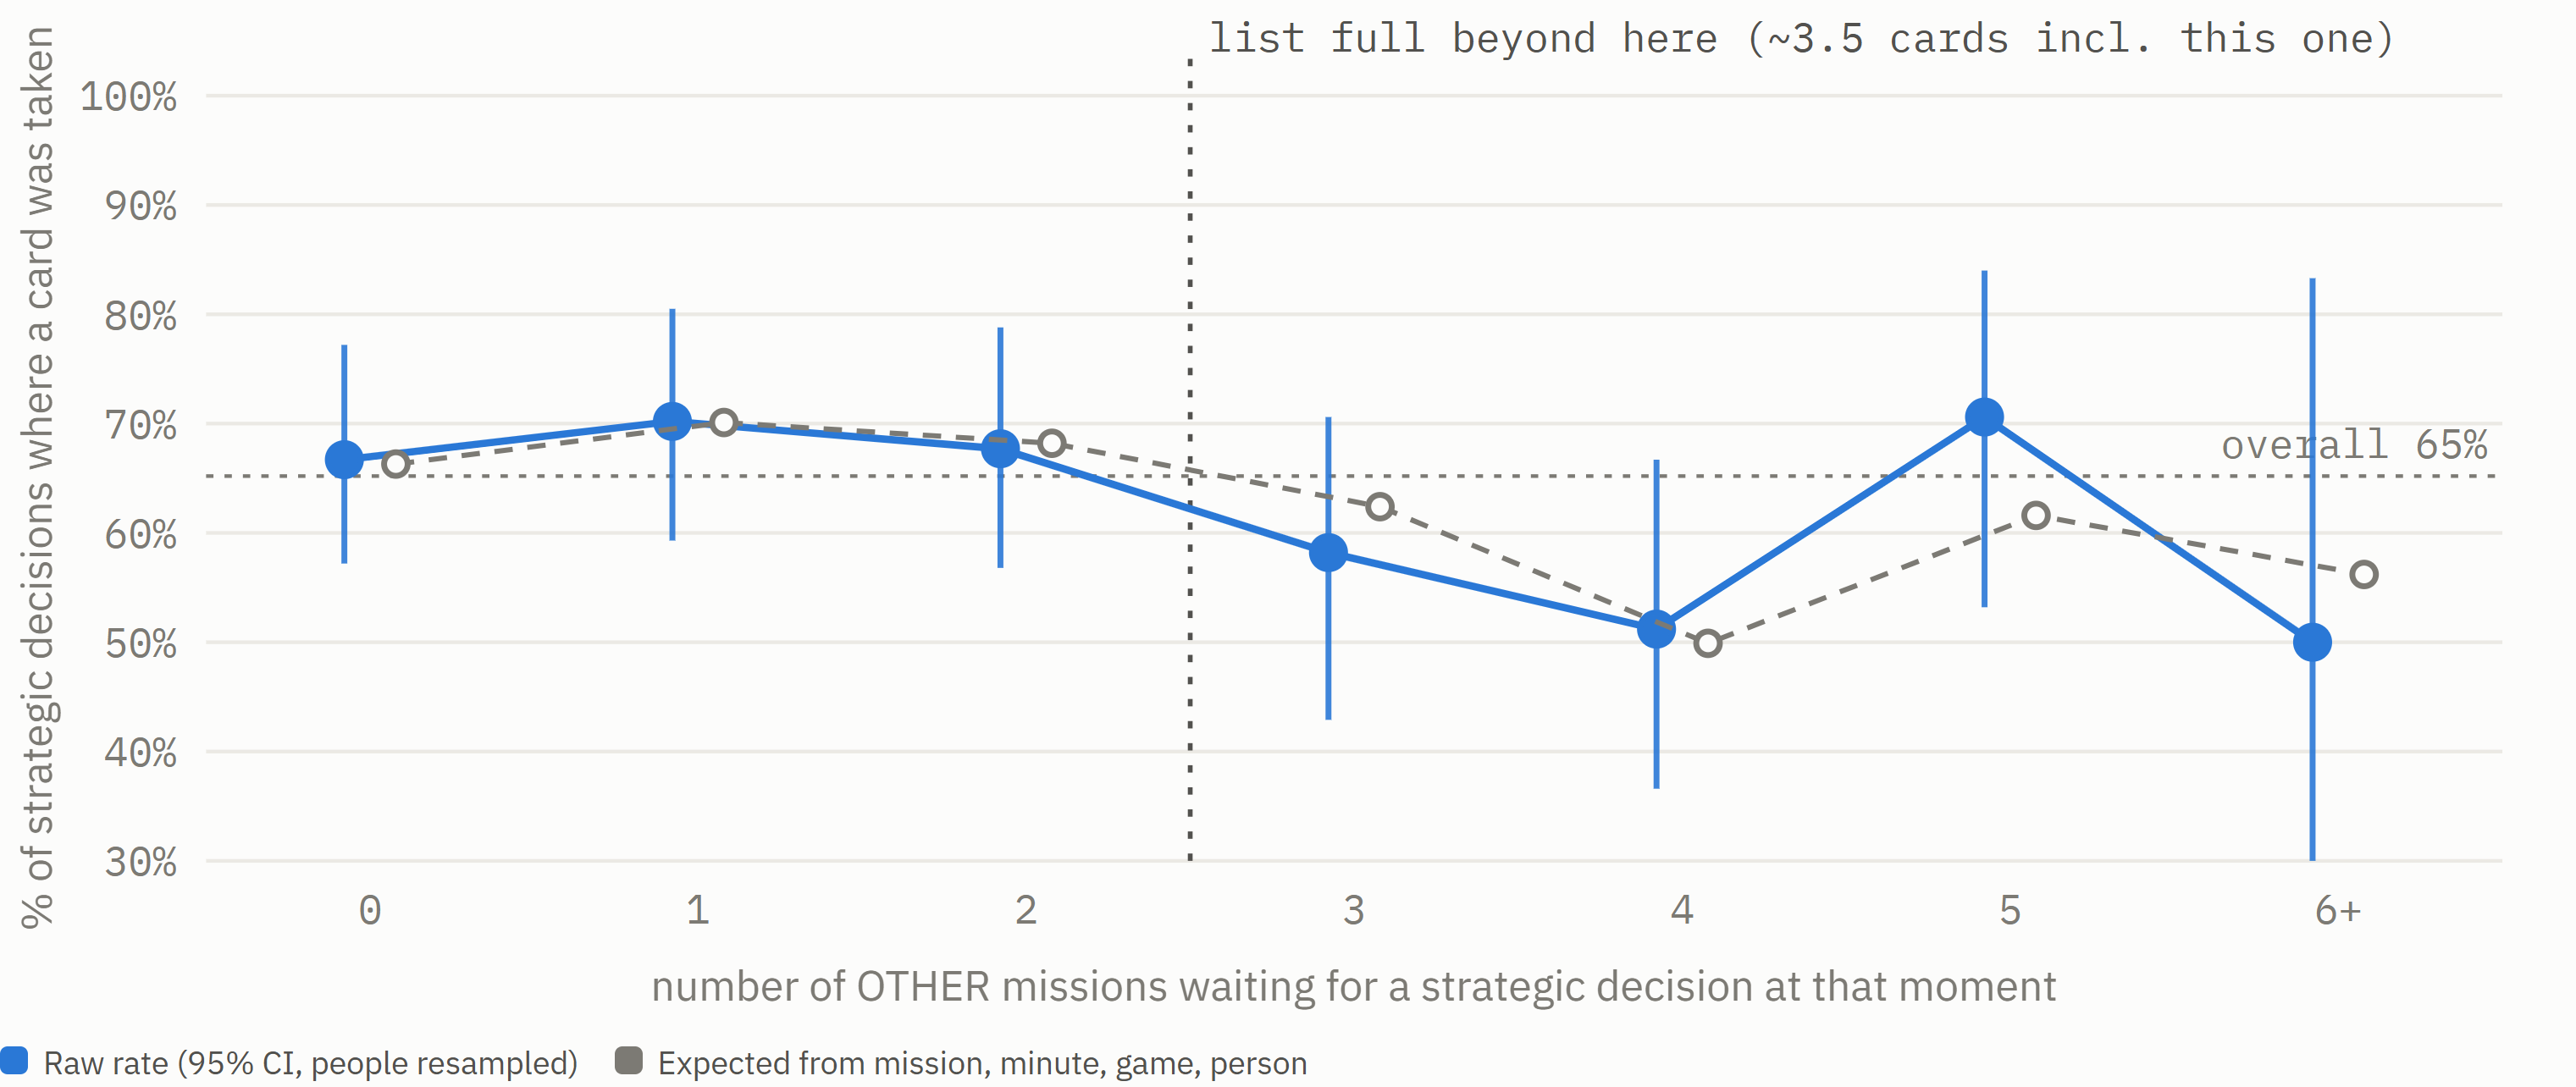
\includegraphics[width=\linewidth,height=0.23\textheight,keepaspectratio]{figs/results/f-workload__raw-vs-adjusted__strat-exp.png}
\caption{Strategic tier, raw with the expected rate (dashed).}
\label{fig:res:workload:raw-vs-adjusted:strat-exp}
\end{subfigure}
\hfill
\begin{subfigure}[t]{0.495\linewidth}
\centering
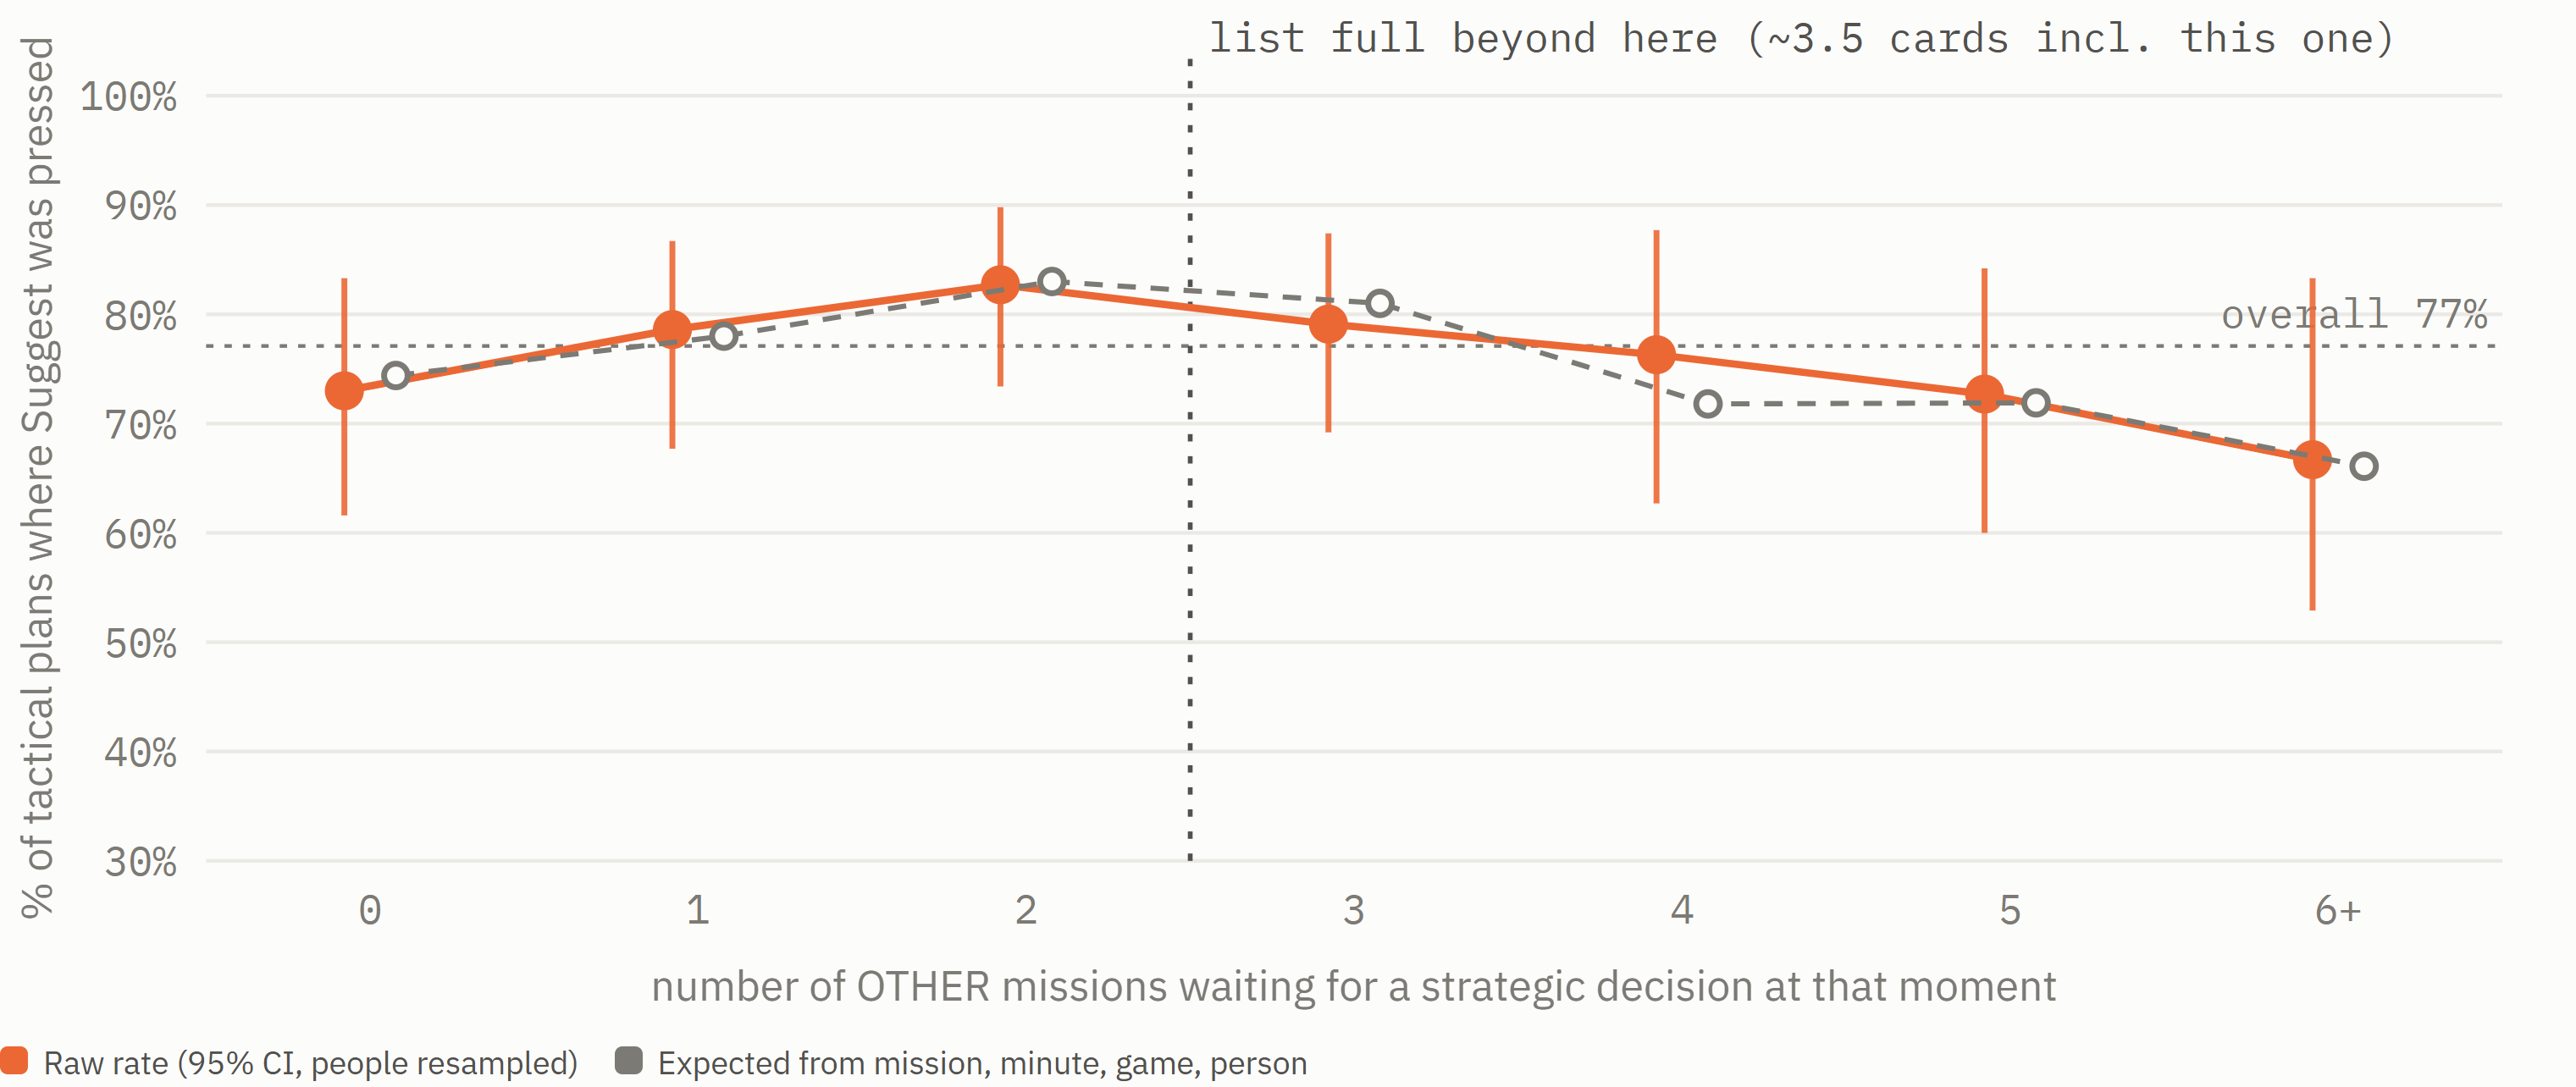
\includegraphics[width=\linewidth,height=0.23\textheight,keepaspectratio]{figs/results/f-workload__raw-vs-adjusted__tac-exp.png}
\caption{Tactical tier, raw with the expected rate (dashed).}
\label{fig:res:workload:raw-vs-adjusted:tac-exp}
\end{subfigure}
\par\smallskip
\caption{\textbf{Queue depth against reliance --- raw, and adjusted}}
\label{fig:res:workload:raw-vs-adjusted}
\end{figure}

\paragraph*{Key numbers.}

\begin{itemize}[leftmargin=1.2em,itemsep=1pt]

\item Strategic raw: 67\% (0 waiting), 70\%, 68\%, 58\%, 51\%, 71\%, 50\% (6+); adjusted: 66\%, 65\%, 65\%, 61\%, 67\%, 74\%, 59\% --- all intervals overlap.

\item Tactical raw: 73\%, 79\%, 83\%, 79\%, 76\%, 73\%, 67\%; adjusted: 76\%, 78\%, 77\%, 75\%, 82\%, 78\%, 78\%.

\item The queue rises with the minute (Spearman $\rho$ = .49) but hardly with mission size ($\rho$ = $-$.08): the adjustment mostly removes WHO reaches deep queues and WHICH GAME they are in.

\item Deep queues are a Strategic Heavy phenomenon: 90--97\% of decisions at 4+ waiting are in those two games.

\end{itemize}

\paragraph*{Method.} {\small \textbf{Rows:} 564 strategic decisions on original (non-residual) missions and 630 tactical plans, 33 people (P09 excluded). \textbf{Queue} = other missions that had arrived and not yet been given a strategic choice when the decision panel opened, rebuilt from the event log (agrees with the logged count for 100\% of decisions). \textbf{Expected}: a logistic model predicts each decision's chance of a card (or Suggest) from four things only --- the mission (drones needed, number of tasks, number of drone types), the minute of the session, the game (one of four fixed scenarios), and the person (their own rate on all their OTHER decisions, so a decision never predicts itself). The queue is deliberately left OUT. \textbf{Adjusted} for a bin = the overall rate + the average of (observed $-$ expected) in that bin. In plain words: 'given who made these decisions, on which missions, at what point in which game, how much more or less did they rely on the assistant than we would expect?' If load mattered, the deep-queue bins would sit above what their missions and people predict; they do not. \textbf{Worked example (strategic, 4 waiting, 41 decisions):} raw 51\% looks like a drop from 67\% at 0 waiting. But 90\% of those decisions were in the two Strategic Heavy games, on missions averaging 6.9 drones (vs 8.7) with fewer three-type missions (54\% vs 66\%), made by people whose usual rate is 56\% (vs 66\%). The model expects 50\%; observed is 51\%; adjusted $\approx$ 67\%. \textbf{Intervals}: people resampled with replacement 400 times, the expected-model re-fitted each time, so the interval includes the uncertainty of the adjustment itself.}

\paragraph*{What participants said.} \regtext{9 of 33 say they hand over more when busy (C11). Almost all of them mean the harder session or 'when workload gets higher', not the moment a queue builds. One clear voice goes against it in play: P18, asked during a stressful session, said 'I think less\ldots{} I'm too focused to look at it'. P21 felt pressure pushed them past the strategy card rather than onto it. P29 and P05 describe pressure as the thing that tips them towards the assistant. That is the claim the adjusted data do not bear out.}

\paragraph*{Quotes selected for this section.}

\begin{quotelist}

\item ``You can have a lot of tasks to be overloaded and try and offload some of that work to AI and then for the very complex stuff, maybe you don't.''\,---\,P20 (debrief 0:28:46)

\item ``So I think if, at first glance, I felt really overwhelmed by the amount of drones to be assigned. I would use the assistant''\,---\,P18 (debrief 0:26:17)

\item ``there was no more active missions coming in, so therefore I could take more time and ensure that it was correct. But perhaps if I was more time pressured, then I'd ask it to suggest.''\,---\,P05 (think-aloud s1 7:31)

\item ``But in an urgent situation and the number of the swarm is not enough, so I need to consider about the strategies and I think I need the help of AI assistant.''\,---\,P35 (debrief 0:28:19)

\item ``I think the first one, I feel the pace is very, very fast. So, I can't do it very well in a very short time. So, I used a lot of AI suggestions.''\,---\,P33 (debrief 0:27:33)

\end{quotelist}

\clearpage

\subsubsection{A mission left waiting is not handed over more often}\label{sec:res:workload:waited}

\noindent \passtag{numbers only}

\noindent \regtext{Do people hand a decision over when they realise they have left it waiting? Here each decision is grouped by how long its mission had been waiting: on the strategic tier, from the mission's arrival to the first time the operator opened it; on the tactical tier, from the planner opening to the operator's first action on it (the plan the operator left sitting while they did something else). \textbf{The lines are flat.} Strategic card use is 63--68\% (adjusted) whether the mission waited 10 seconds or more than two minutes. Tactical Suggest use, if anything, drifts down when a plan was left open longer (80\% $\rightarrow$ 70\%), the opposite of the idea, but not reliably.} (Figure~\ref{fig:res:workload:waited})

\begin{figure}[H]
\centering
\begin{subfigure}[t]{\linewidth}
\centering
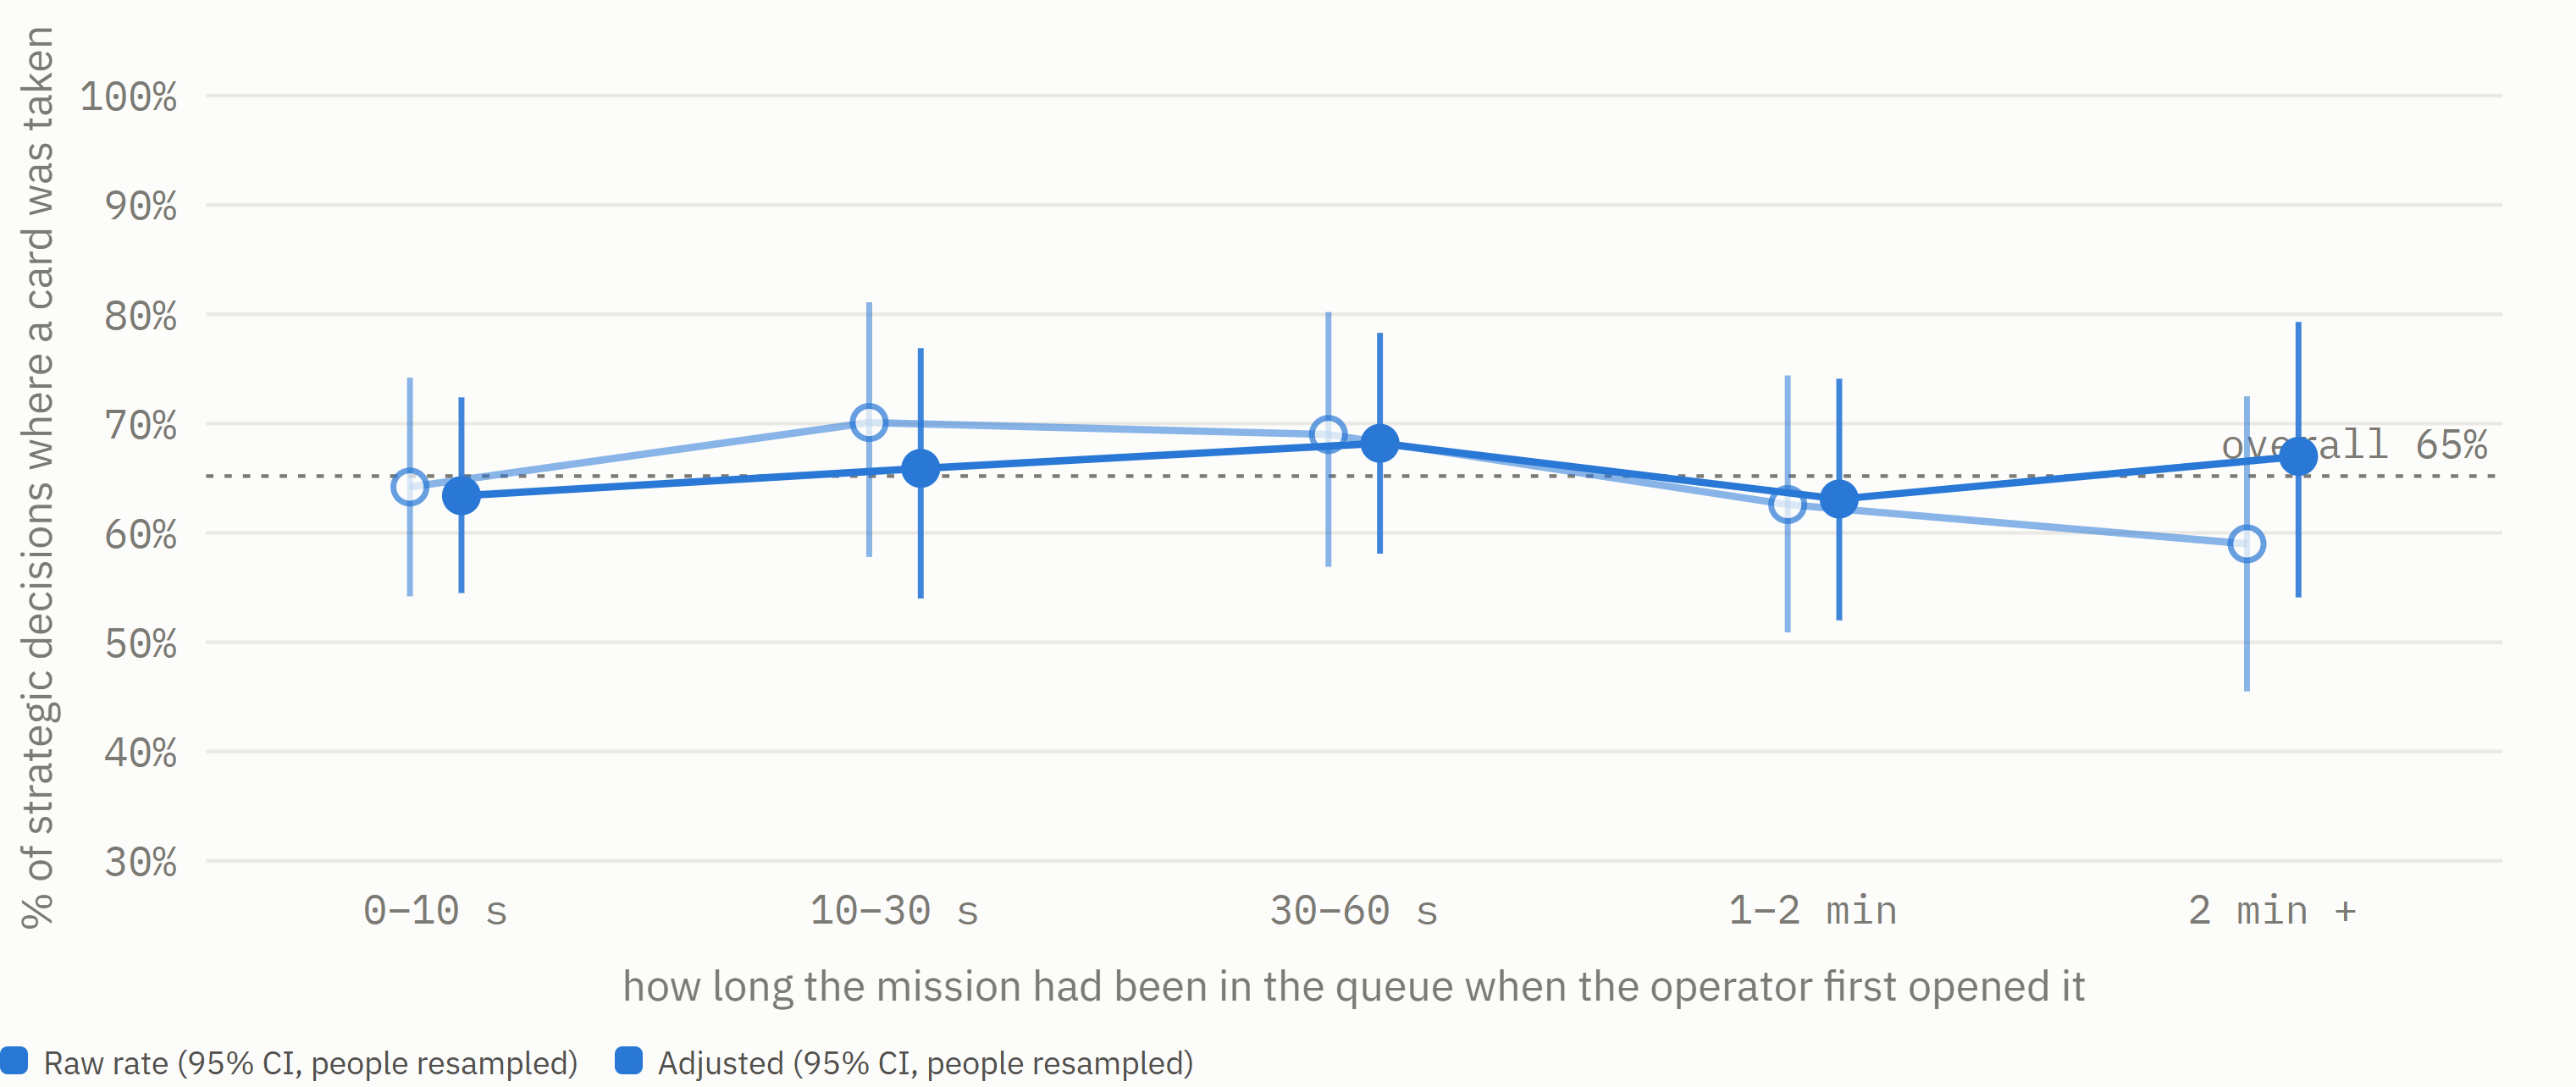
\includegraphics[width=\linewidth,height=0.23\textheight,keepaspectratio]{figs/results/f-workload__waited__strat.png}
\caption{Strategic tier: how long the mission had waited in the queue.}
\label{fig:res:workload:waited:strat}
\end{subfigure}
\par\smallskip
\begin{subfigure}[t]{\linewidth}
\centering
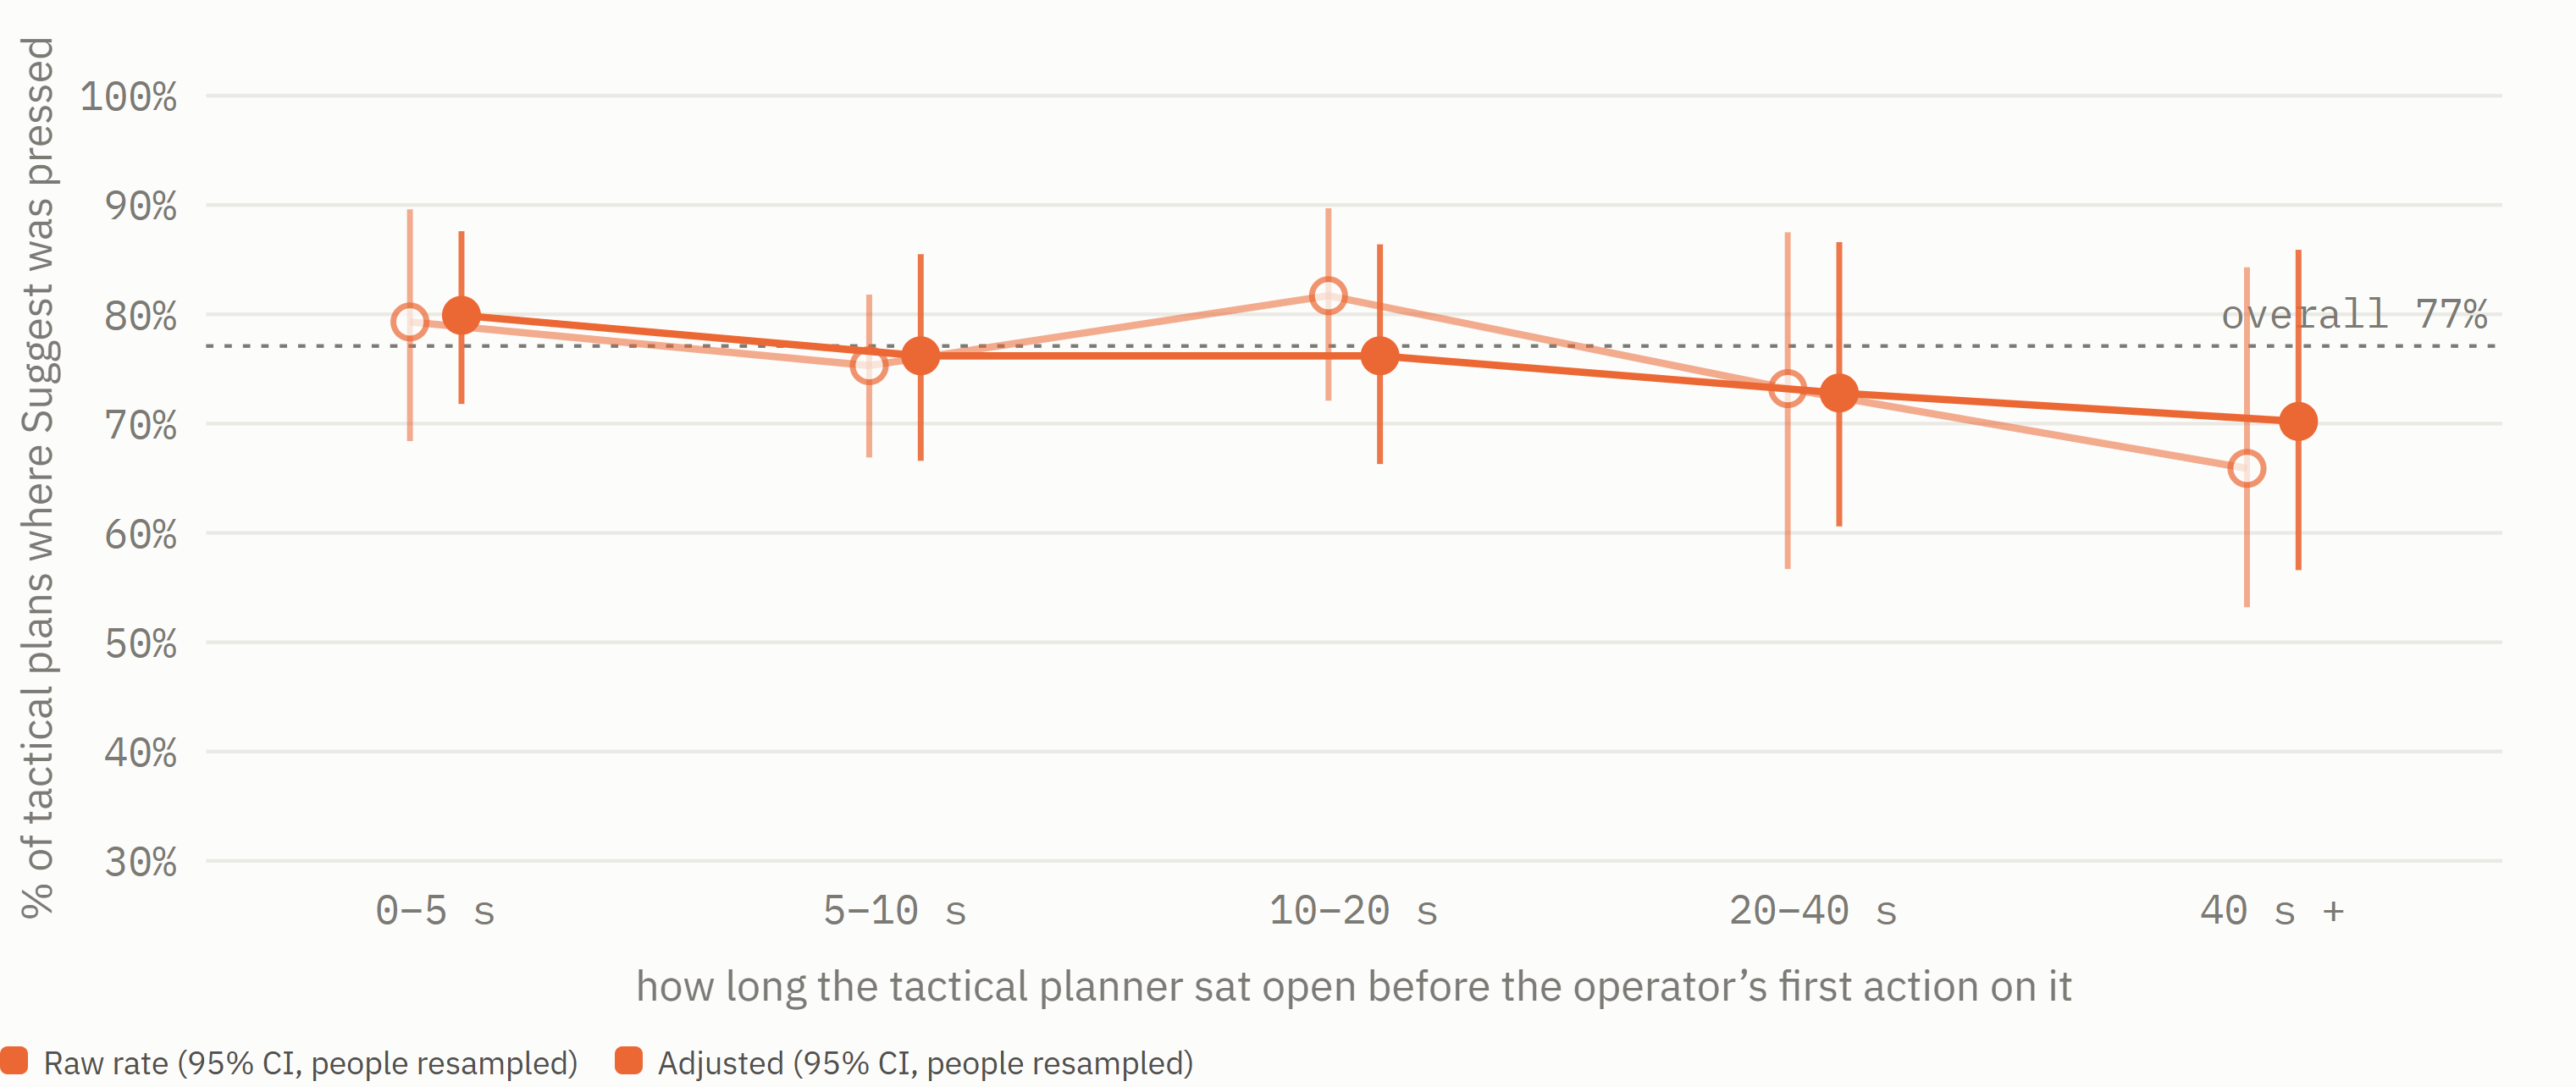
\includegraphics[width=\linewidth,height=0.23\textheight,keepaspectratio]{figs/results/f-workload__waited__tac.png}
\caption{Tactical tier: how long the plan had been left open.}
\label{fig:res:workload:waited:tac}
\end{subfigure}
\par\smallskip
\caption{\textbf{A mission left waiting is not handed over more often}}
\label{fig:res:workload:waited}
\end{figure}

\paragraph*{Key numbers.}

\begin{itemize}[leftmargin=1.2em,itemsep=1pt]

\item Strategic (mission left in the queue): adjusted 63\% at 0--10 s, 66\% 10--30 s, 68\% 30--60 s, 63\% 1--2 min, 67\% at 2 min+ (n 173, 117, 100, 91, 83). Within person, odds $\times$1.10 per doubling of the wait [0.96, 1.28], p = .17; holding the queue fixed $\times$1.10, p = .19.

\item Tactical (plan left open): adjusted 80\% at 0--5 s, 76\% 5--10 s, 76\% 10--20 s, 73\% 20--40 s, 70\% at 40 s+ (n 270, 182, 93, 41, 44). Within person, odds $\times$0.80 per doubling [0.60, 1.06], p = .12; holding the queue fixed $\times$0.76, p = .10.

\end{itemize}

\paragraph*{Method.} {\small Rows: every strategic decision on a real (not re-queued) mission, 564 from 33 people, and every tactical plan, 630. Wait: strategic, mission arrival to the first time its strategy panel was opened; tactical, planner open to the first drag or Suggest. 'Adjusted' is the overall rate plus the average of (observed $-$ expected) in that bin, where the expected value comes from mission size and drone types, minute of the session, the game and the person's own rate on their other decisions (the same model as section 1). Intervals resample people. The odds ratio compares each person with themselves: log2 of the wait (+5 s), centred within person, in a model with the same controls, people clustered; a second version also holds the queue depth fixed, since long waits come at busy moments.}

\clearpage

\subsection{Busy operators speed up a little but do not change what they pick}\label{sec:res:triage}

\regtext{\textbf{Summary.} The earlier story --- that with a long queue operators abandon order and pick smaller missions --- does not survive a fair comparison. Long queues happen almost only in the two Strategic Heavy games, where every mission is small, so the opened mission is smaller simply because everything waiting is. Compared with what was actually waiting, operators keep the same priorities at any queue length: a strong pull towards the oldest mission, a mild preference for larger ones, and only falling 'oldest-first' rates because chance falls as more missions wait. What does change is pace: a bit more decisions per minute when more is waiting (suggestive).} \par\noindent{\small\textit{Strength of evidence (register rating): mixed. Your verdict: keep.}}

\subsubsection{Order: still oldest-first well above chance}\label{sec:res:triage:order}

\noindent \passtag{for the paper}

\noindent \regtext{The share of decisions that open the oldest waiting mission falls as the queue grows (59\% with one other waiting, about 30\% with five) --- but so does the chance of hitting the oldest by picking at random (50\% $\rightarrow$ 17\%). Measured against chance, the pull towards the oldest stays roughly the same. 'One of the top 3 in the list' is near chance at every depth, so the list position itself does little beyond 'oldest first'.} (Figure~\ref{fig:res:triage:order})

\begin{figure}[H]
\centering
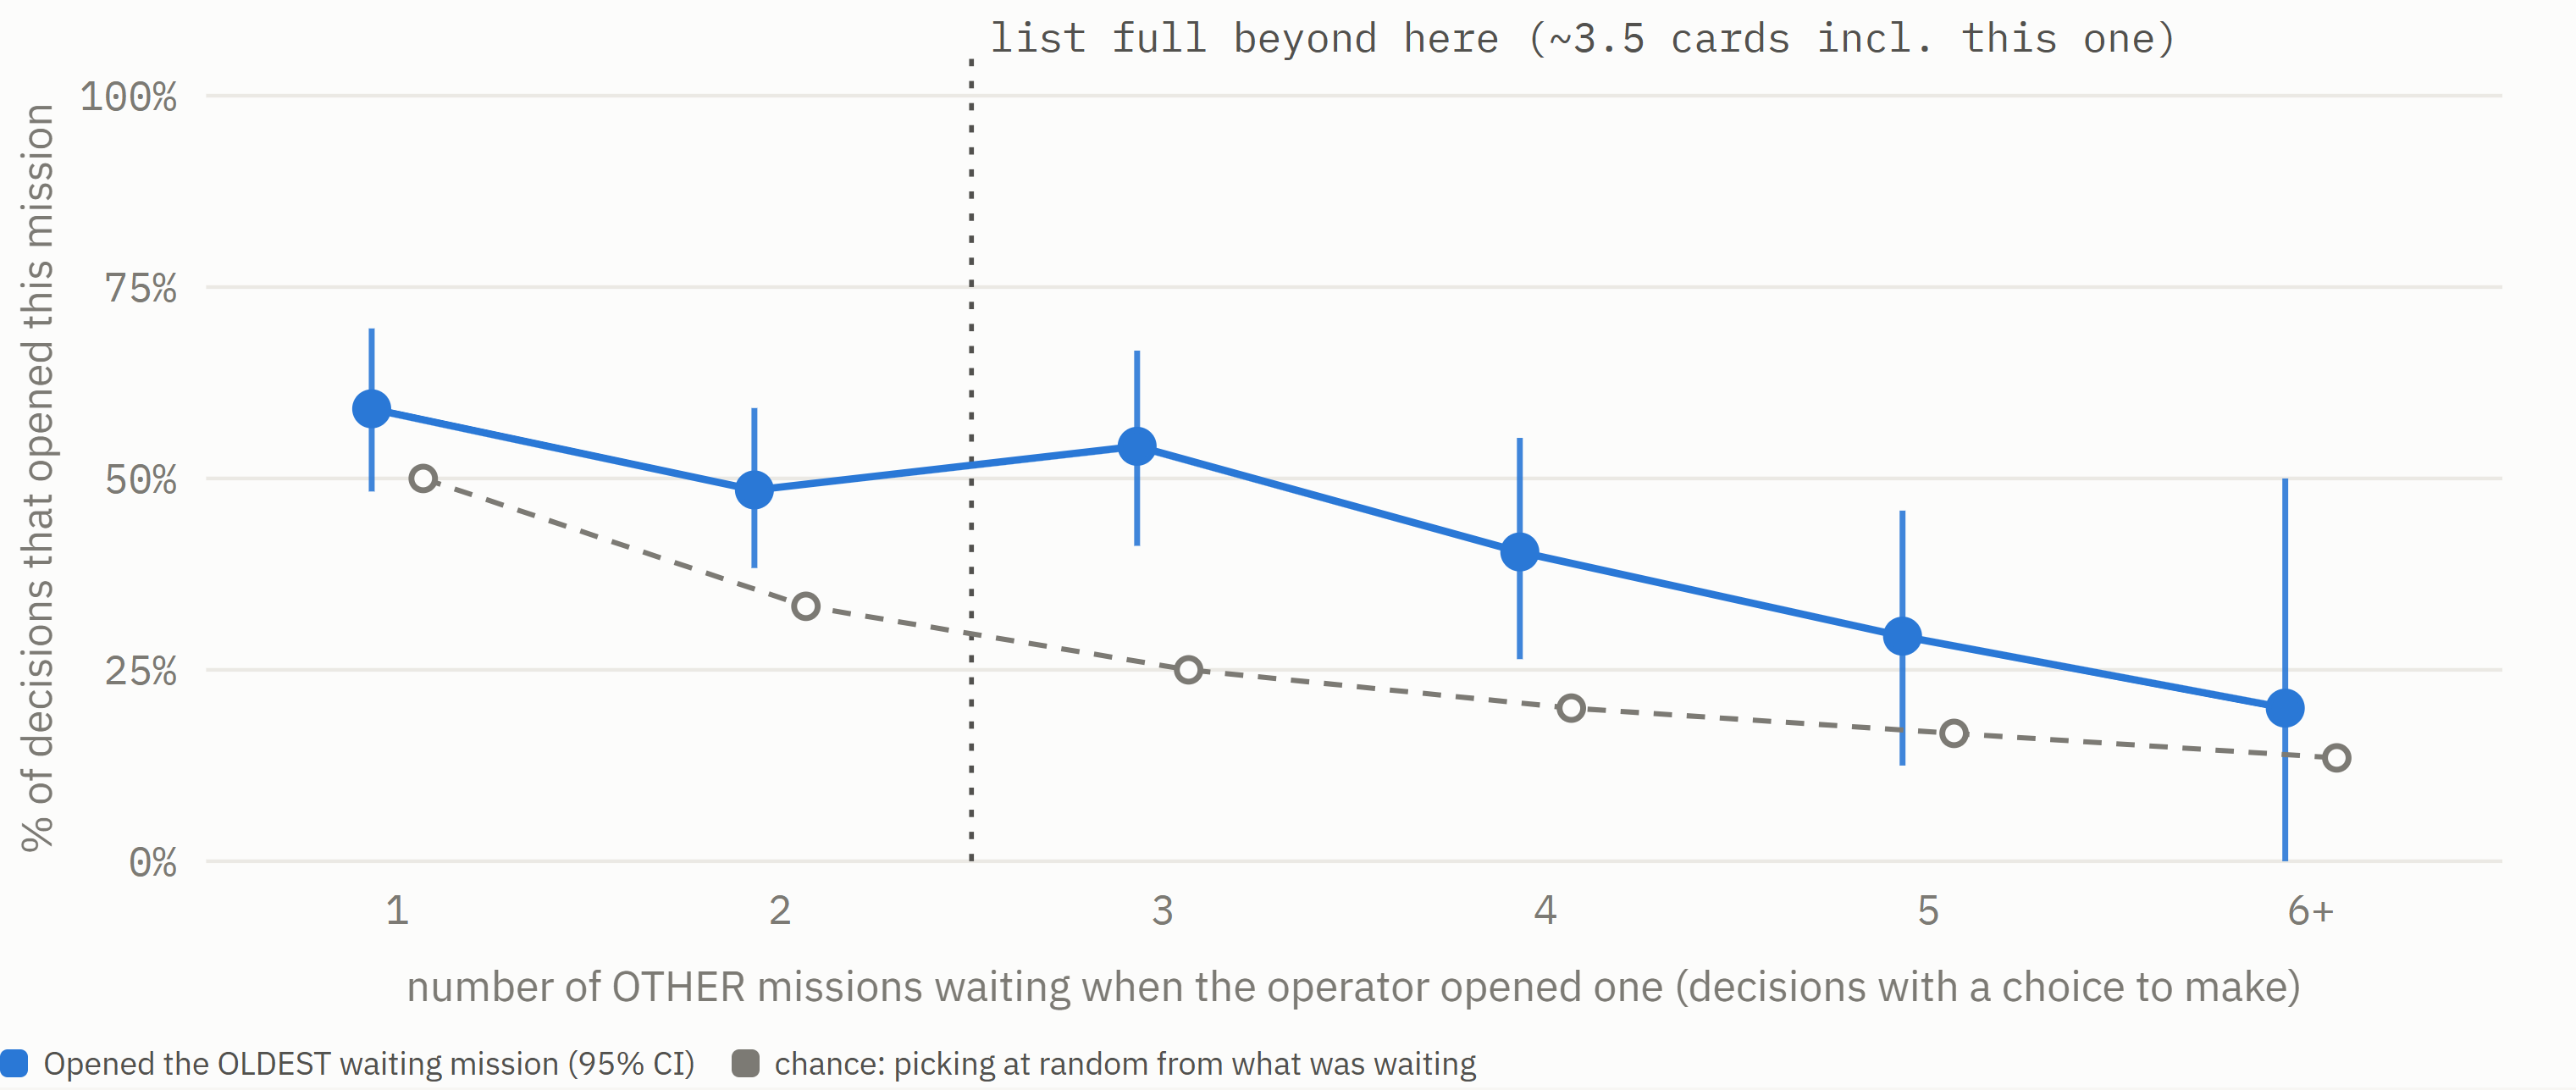
\includegraphics[width=\linewidth,height=0.55\textheight,keepaspectratio]{figs/results/f-triage__order__main.png}
\caption{\textbf{Order: still oldest-first well above chance}}
\label{fig:res:triage:order}
\end{figure}

\paragraph*{Key numbers.}

\begin{itemize}[leftmargin=1.2em,itemsep=1pt]

\item Opened the oldest: 59\% (1 other waiting; chance 50\%), 48\% (33\%), 54\% (25\%), 40\% (20\%), 29\% (17\%), 20\% (14\%).

\item Within person, the excess over chance does not shrink with depth: +2.4 points per extra mission [$-$1.0, +5.7], p = .16.

\end{itemize}

\paragraph*{Method.} {\small 414 strategic decisions where at least one other mission was waiting (33 people). For each, the set of missions waiting when the panel opened (arrival order from the log). Chance = 1 / (number waiting) for 'oldest'; 3 / (number waiting) for 'top 3'. Intervals: people resampled 400 times. Within-person test: (picked oldest $-$ chance) against queue depth, person-centred, with minute and game. Caveat: the list could be re-sorted by score and that toggle was never logged.}

\paragraph*{What participants said.} \regtext{Nobody says they took missions oldest-first. Five say, in play or after, that criticality comes first ('I'll go with the most critical first'): P20, P22, P31, P19 and P27. P27 adds 'can it be completed' as the first filter. The order model has no criticality term, so this stated rule is untested. P19 wished for a sort control, and P27 for smart ordering, unaware that an order-by-criticality button existed.}

\clearpage

\subsubsection{What makes a waiting mission get opened, short vs long queues}\label{sec:res:triage:choice}

\noindent \passtag{numbers only}

\noindent \regtext{Putting it together in one model of the choice among what was waiting: being the oldest roughly triples a mission's chance of being opened, larger missions are mildly preferred, and being the newest arrival helps a little. These pulls are statistically clear where marked, and none of them changes significantly between short (1--3 others waiting) and long (4+) queues: the ``long $\div$ short'' rows all have intervals spanning 1. Under pressure, priorities do not visibly change, though with 95 long-queue decisions only a large change could have been detected.} (Figure~\ref{fig:res:triage:choice})

\begin{figure}[H]
\centering
\begin{subfigure}[t]{\linewidth}
\centering
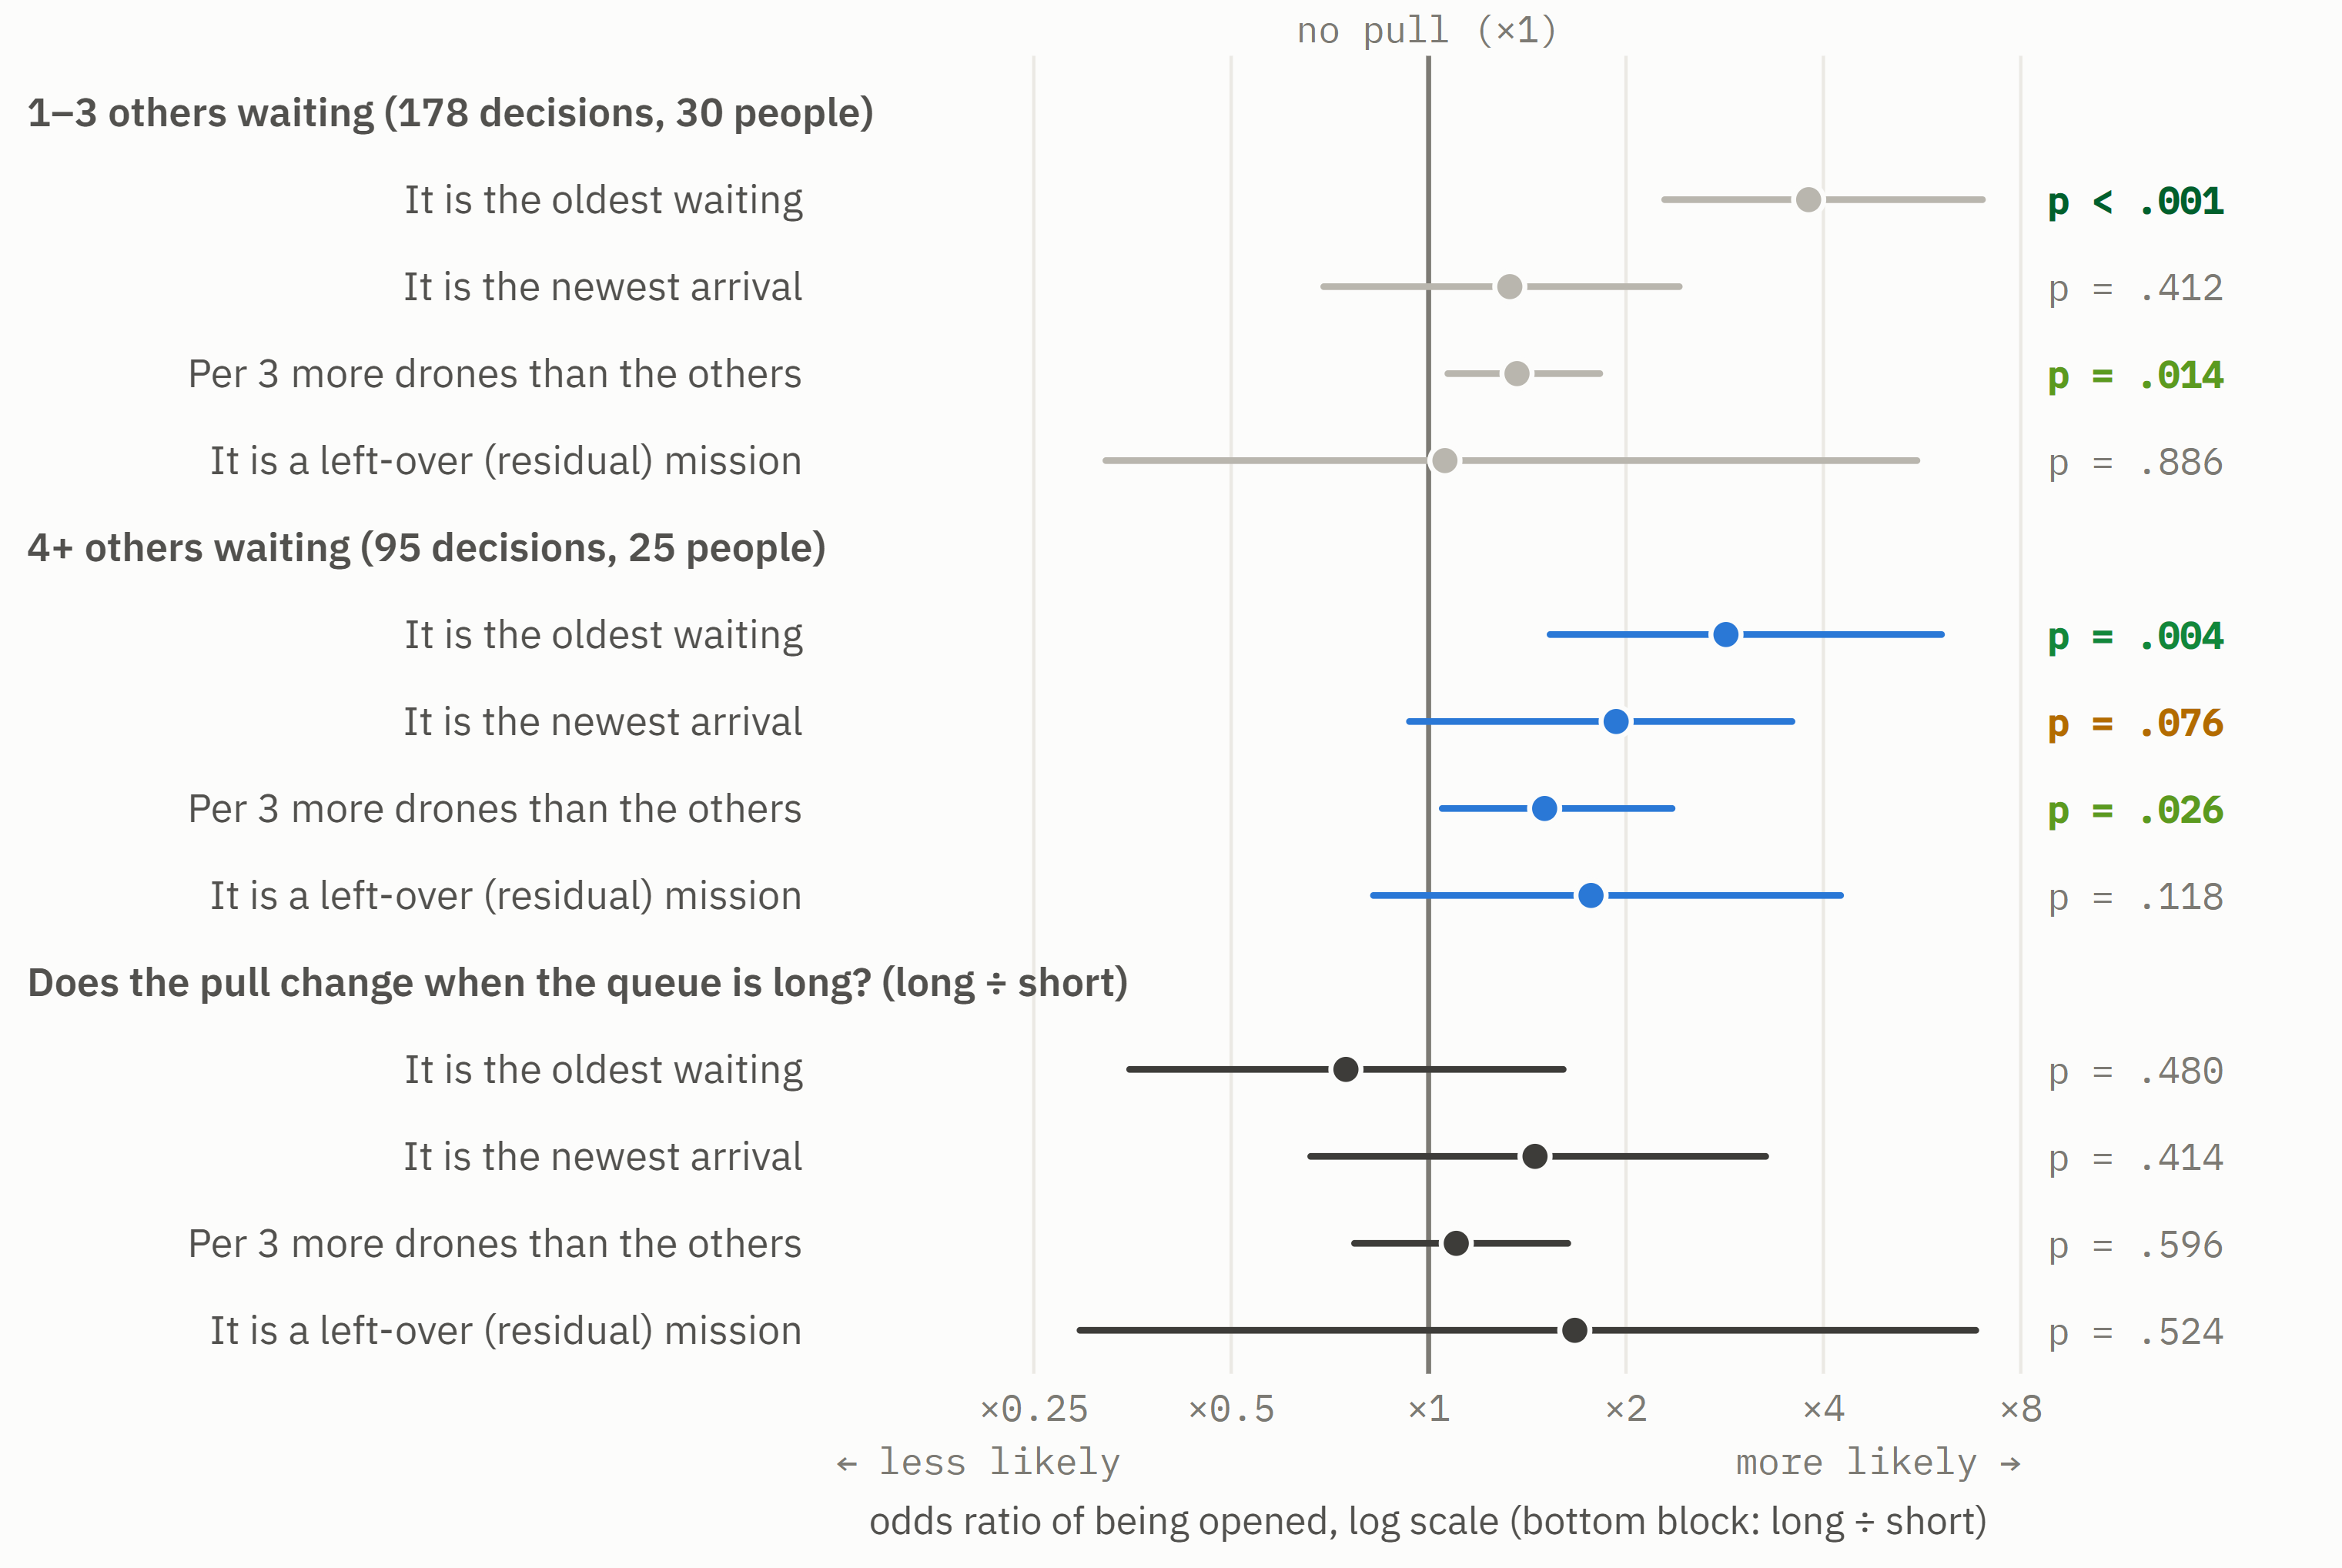
\includegraphics[width=\linewidth,height=0.23\textheight,keepaspectratio]{figs/results/f-triage__choice__sh.png}
\caption{Strategic Heavy games only.}
\label{fig:res:triage:choice:sh}
\end{subfigure}
\par\smallskip
\begin{subfigure}[t]{\linewidth}
\centering
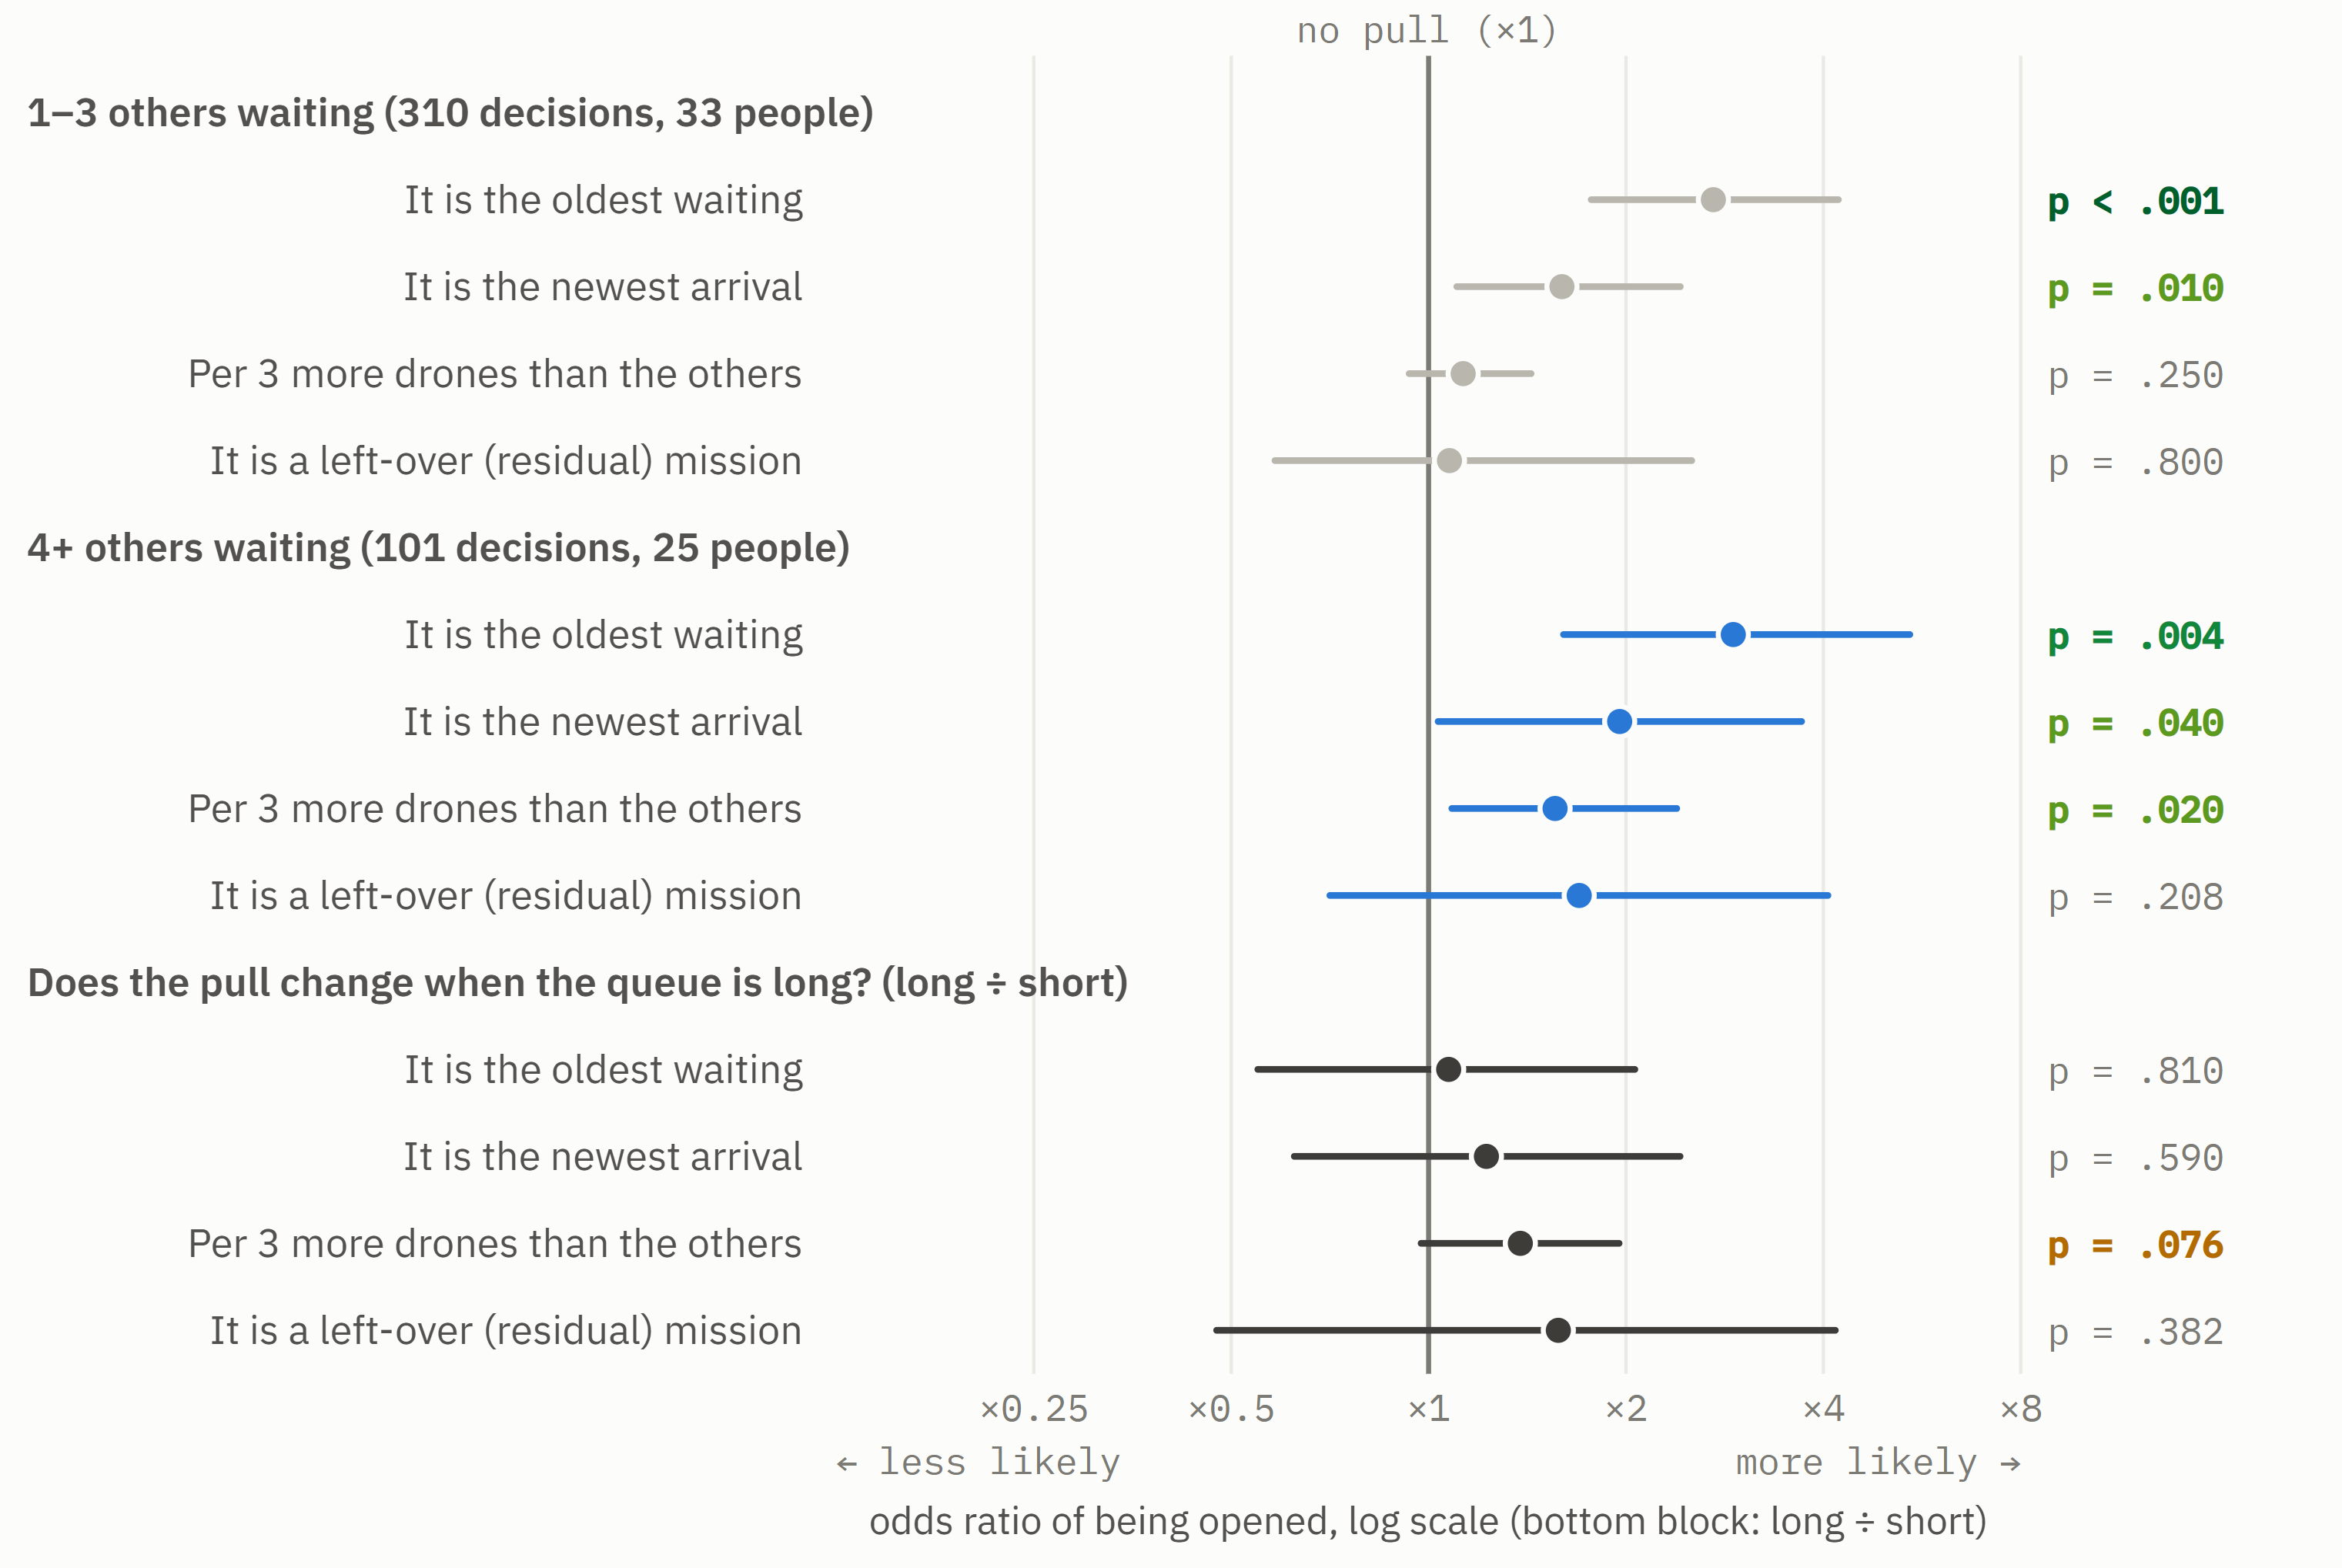
\includegraphics[width=\linewidth,height=0.23\textheight,keepaspectratio]{figs/results/f-triage__choice__all.png}
\caption{All four games.}
\label{fig:res:triage:choice:all}
\end{subfigure}
\par\smallskip
\caption{\textbf{What makes a waiting mission get opened, short vs long queues}}
\label{fig:res:triage:choice}
\end{figure}

\paragraph*{Key numbers.}

\begin{itemize}[leftmargin=1.2em,itemsep=1pt]

\item Strategic Heavy games, short queues (178 decisions): oldest $\times$3.80 [2.29, 6.99], p < .001; newest $\times$1.33 [0.69, 2.41], p = .41; +3 drones $\times$1.36 [1.07, 1.82], p = .014; residual $\times$1.06, p = .89

\item Strategic Heavy games, long queues (95 decisions): oldest $\times$2.84 [1.53, 6.06], p = .004; newest $\times$1.93 [0.94, 3.58], p = .076; +3 drones $\times$1.50 [1.05, 2.35], p = .026; residual $\times$1.77, p = .12

\item Long $\div$ short, Strategic Heavy games: oldest $\times$0.75 [0.35, 1.60], p = .48; newest $\times$1.45, p = .41; size $\times$1.10, p = .60; residual $\times$1.67, p = .52 (none differs)

\item All four games: oldest $\times$2.72 (short) and $\times$2.92 (long), both p $\leq$ .004; newest $\times$1.60, p = .010 and $\times$1.96, p = .040; size $\times$1.13, p = .25 and $\times$1.56, p = .020; long $\div$ short for size $\times$1.38 [0.97, 1.95], p = .076, all others p $\geq$ .38

\end{itemize}

\paragraph*{Method.} {\small Conditional logit: each decision is a choice among the missions waiting at that moment; the model estimates how much each feature (oldest, newest, size relative to the set in units of 3 drones, residual) multiplies a mission's odds of being the one opened. Fitted separately for short (1--3 others) and long (4+) queues, in the Strategic Heavy games only (like with like) and in all four. Intervals and p-values: people resampled 1000 times (the short- and long-queue fits on the same resampled people), so they allow for each person making many decisions; p = twice the share of resamples on the far side of ``no pull''. The ``long $\div$ short'' rows are the ratio of the two odds ratios with their own interval and p, i.e. a direct test of whether the pull changes with the queue.}

\paragraph*{What participants said.} \regtext{Besides criticality, people describe choosing by feasibility: they skip what the reserve cannot cover yet and come back (P17, P27, P30). P19 jumped to a newly arrived higher-priority mission, which matches the small 'newest' pull. Nobody mentions preferring larger missions, and nobody says their way of choosing changed when the queue was long.}

\clearpage

\subsection{The dip in strategy-card use belongs to the people who later said they noticed the illogical card, early in the session; it shows up whether or not they had met that card yet}\label{sec:res:flaw-odd}

\regtext{\textbf{Summary.} The Conservative card sometimes adds a drone type the mission does not use (22\% of decisions, nearly all on one-type missions); all 33 people met it, usually on their 1st or 2nd decision. The 15 who said they noticed it take the cards less afterwards, and on the flawed one-type missions they learn to skip them (0 takes in 13 by their 4th--6th such mission). But the \textbf{dip} in their use is not tied to the card. Counted simply by decision number, noticers take the cards on 80\% of their 1st session-1 decision and 46--50\% of decisions 3--5, then 83\% at decision 6, while never-said people rise to 89--94\% in the same stretch. People who played the tactical-heavy game first had \emph{not yet met} an illogical card in decisions 3--5 (95\% of those decisions came before it), and their noticers dip just as much ($-$21 points per person, against $-$32 for those who had met it; game order makes no difference, p = .79). In that stretch noticers look at the cards and turn them down, on three-type missions too. Pooled over everyone the dip disappears, because the two groups move in opposite directions. Noticers climb back later in session 1 (+24 points per person) and start session 2 lower again (49\%), but never-said people also start session 2 a little lower, so a weaker carry-over for noticers is not something these data can show (difference at the break $-$6 points [$-$32, +20]). Our best reading: ``noticed'' marks people who scrutinise the cards, and the dip is that scrutiny at the first busy stretch of the study, not a reaction to the illogical card. What triggers it at that moment we cannot say: mission mix, load, reserve shortage and game do not account for it. Suggestive (15 vs 18 people, window read off the curve). This finding also holds, sidelined, the flaw-visibility comparison and the recovery material merged in from two other findings.} \par\noindent{\small\textit{Strength of evidence (register rating): suggestive. Your verdict: core.}}

\subsubsection{The event study, aligned on the first illogical card (every step, pairs or threes)}\label{sec:res:flaw-odd:event}

\noindent \passtag{for the paper}

\noindent \regtext{Each person's decisions are numbered \emph{within} the kind of mission plotted: their 1st, 2nd, \ldots{} decision after the first illogical card. With every step shown, each point is then about 15 single decisions and its interval spans roughly 30 points either way. Pairs keep the shape with intervals about a third narrower, so pairs is the default. On \textbf{all missions}, noticers go from 76\% before the card to 43--52\% for their next ten decisions, recovering to 67--68\% only from the 11th on. Never-said people stay at 67--75\% throughout. Part of the noticers' low on all missions is the flawed one-type missions themselves, where they increasingly refuse the card. On \textbf{three-type missions}, noticers go 74\% $\rightarrow$ 43\% (1st--2nd) $\rightarrow$ 59--63\% $\rightarrow$ 75\%: a short dip and recovery. On one- and two-type missions almost nobody has a decision before the card, because the card only ever appears there, so only the after-card trend can be read. \textbf{The steps before the card} add little: most people have only one decision before it, so $-$2 and $-$3 are 8 decisions each ($\pm$35 points). The last step before the card ($-$1) is lower than $-$3/$-$2 in \emph{both} groups (64\% and 56\%), so it is not a noticer warning sign. \textbf{Read with the next section:} the aligned dip is not where it seems.} (Figure~\ref{fig:res:flaw-odd:event})

\begin{figure}[H]
\centering
\begin{subfigure}[t]{\linewidth}
\centering
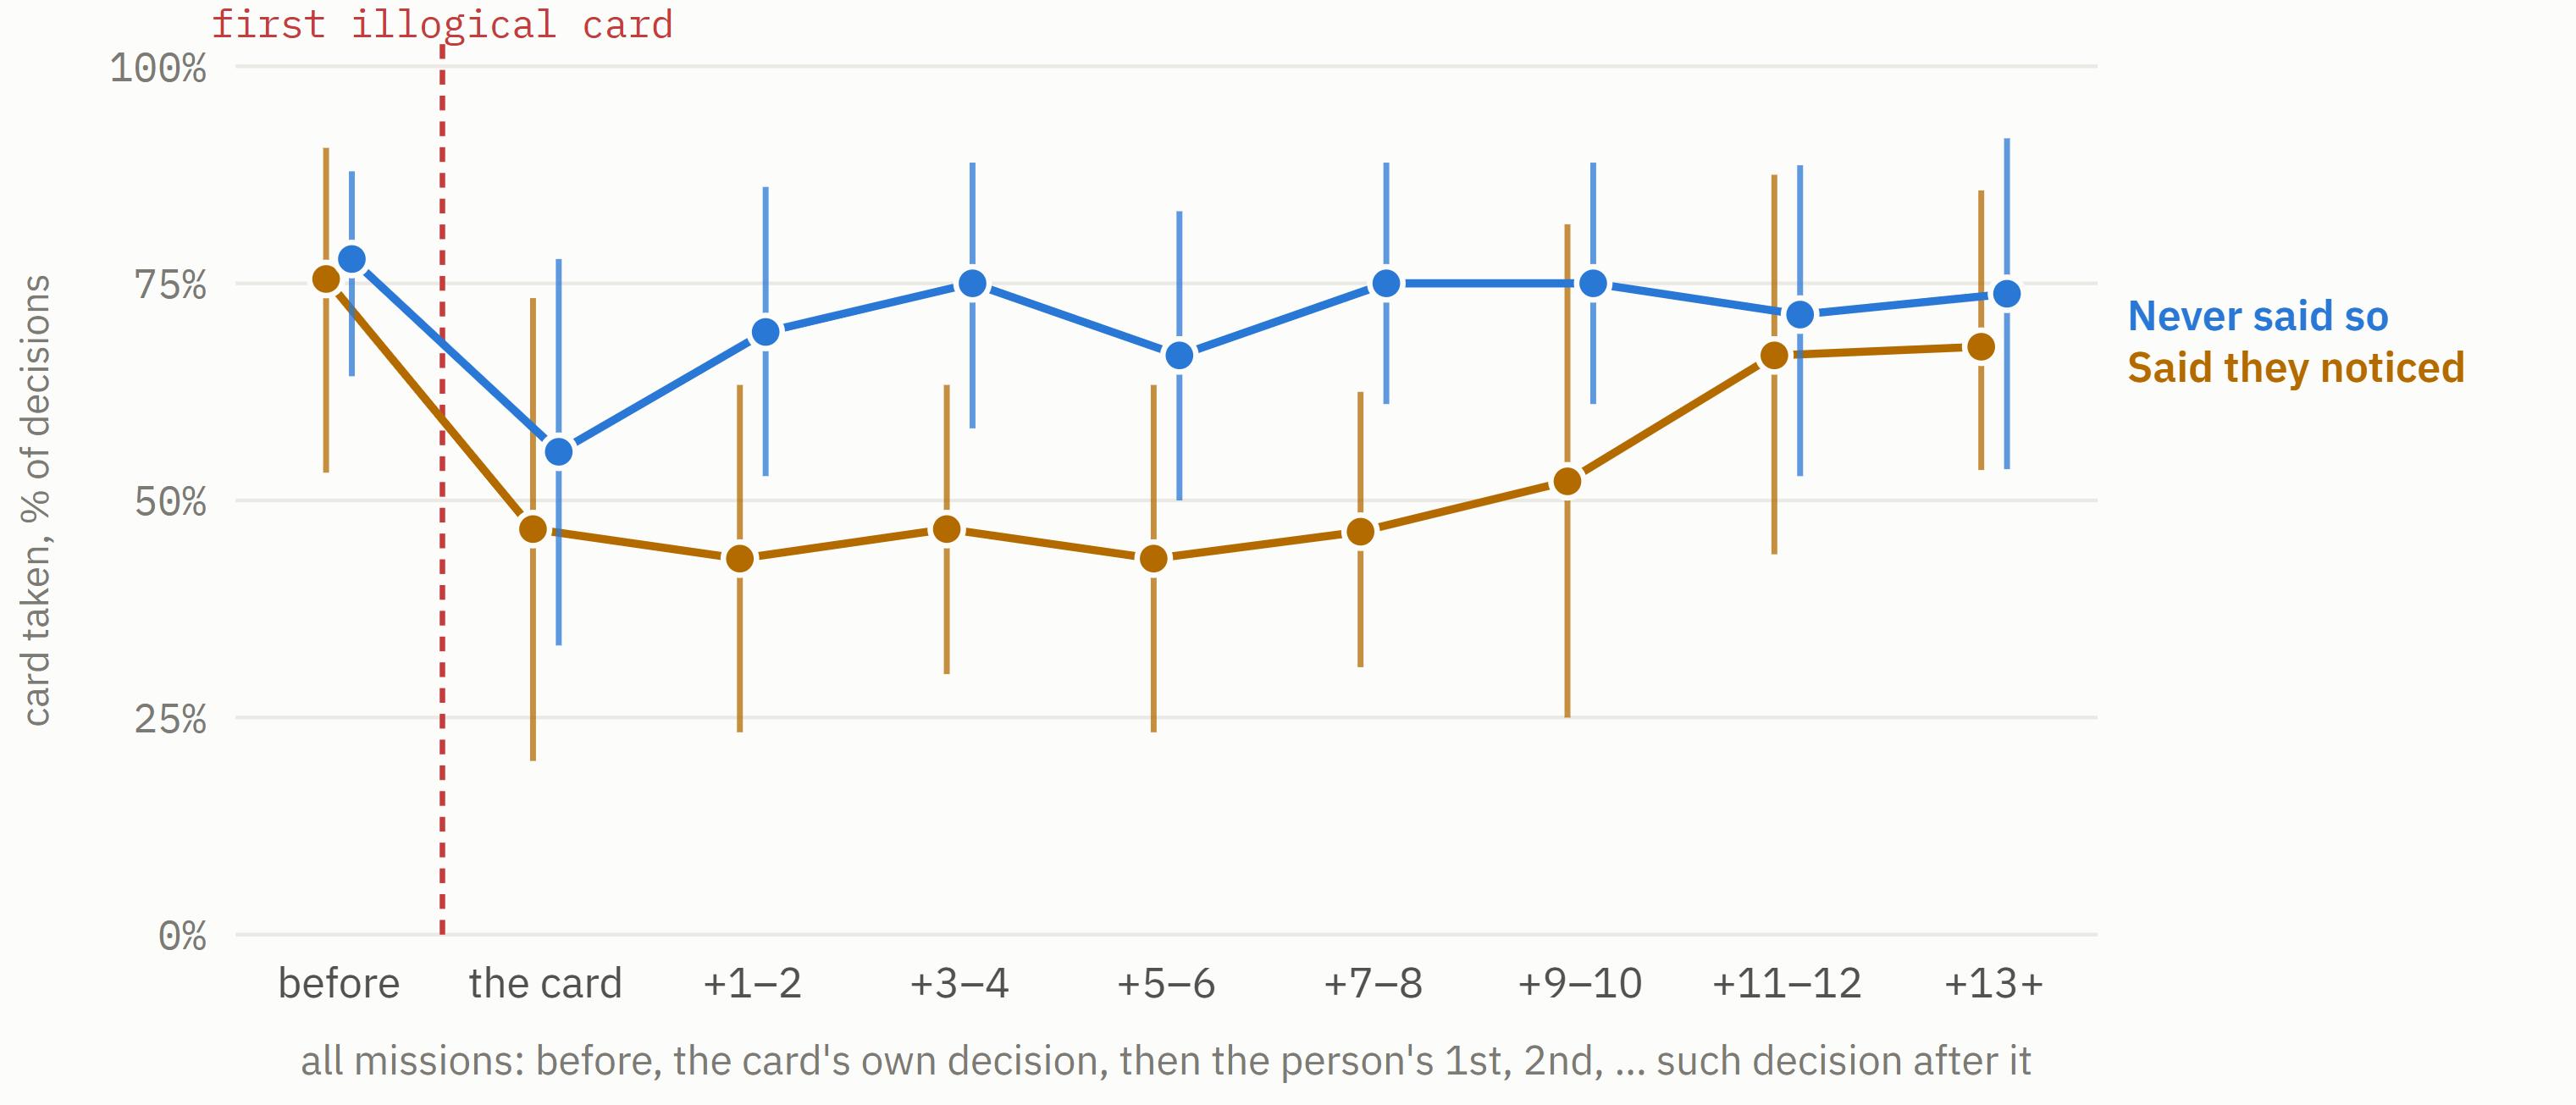
\includegraphics[width=\linewidth,height=0.23\textheight,keepaspectratio]{figs/results/f-flaw-odd__event__pairs.png}
\caption{All missions, every pair of decisions, observed.}
\label{fig:res:flaw-odd:event:pairs}
\end{subfigure}
\par\smallskip
\begin{subfigure}[t]{\linewidth}
\centering
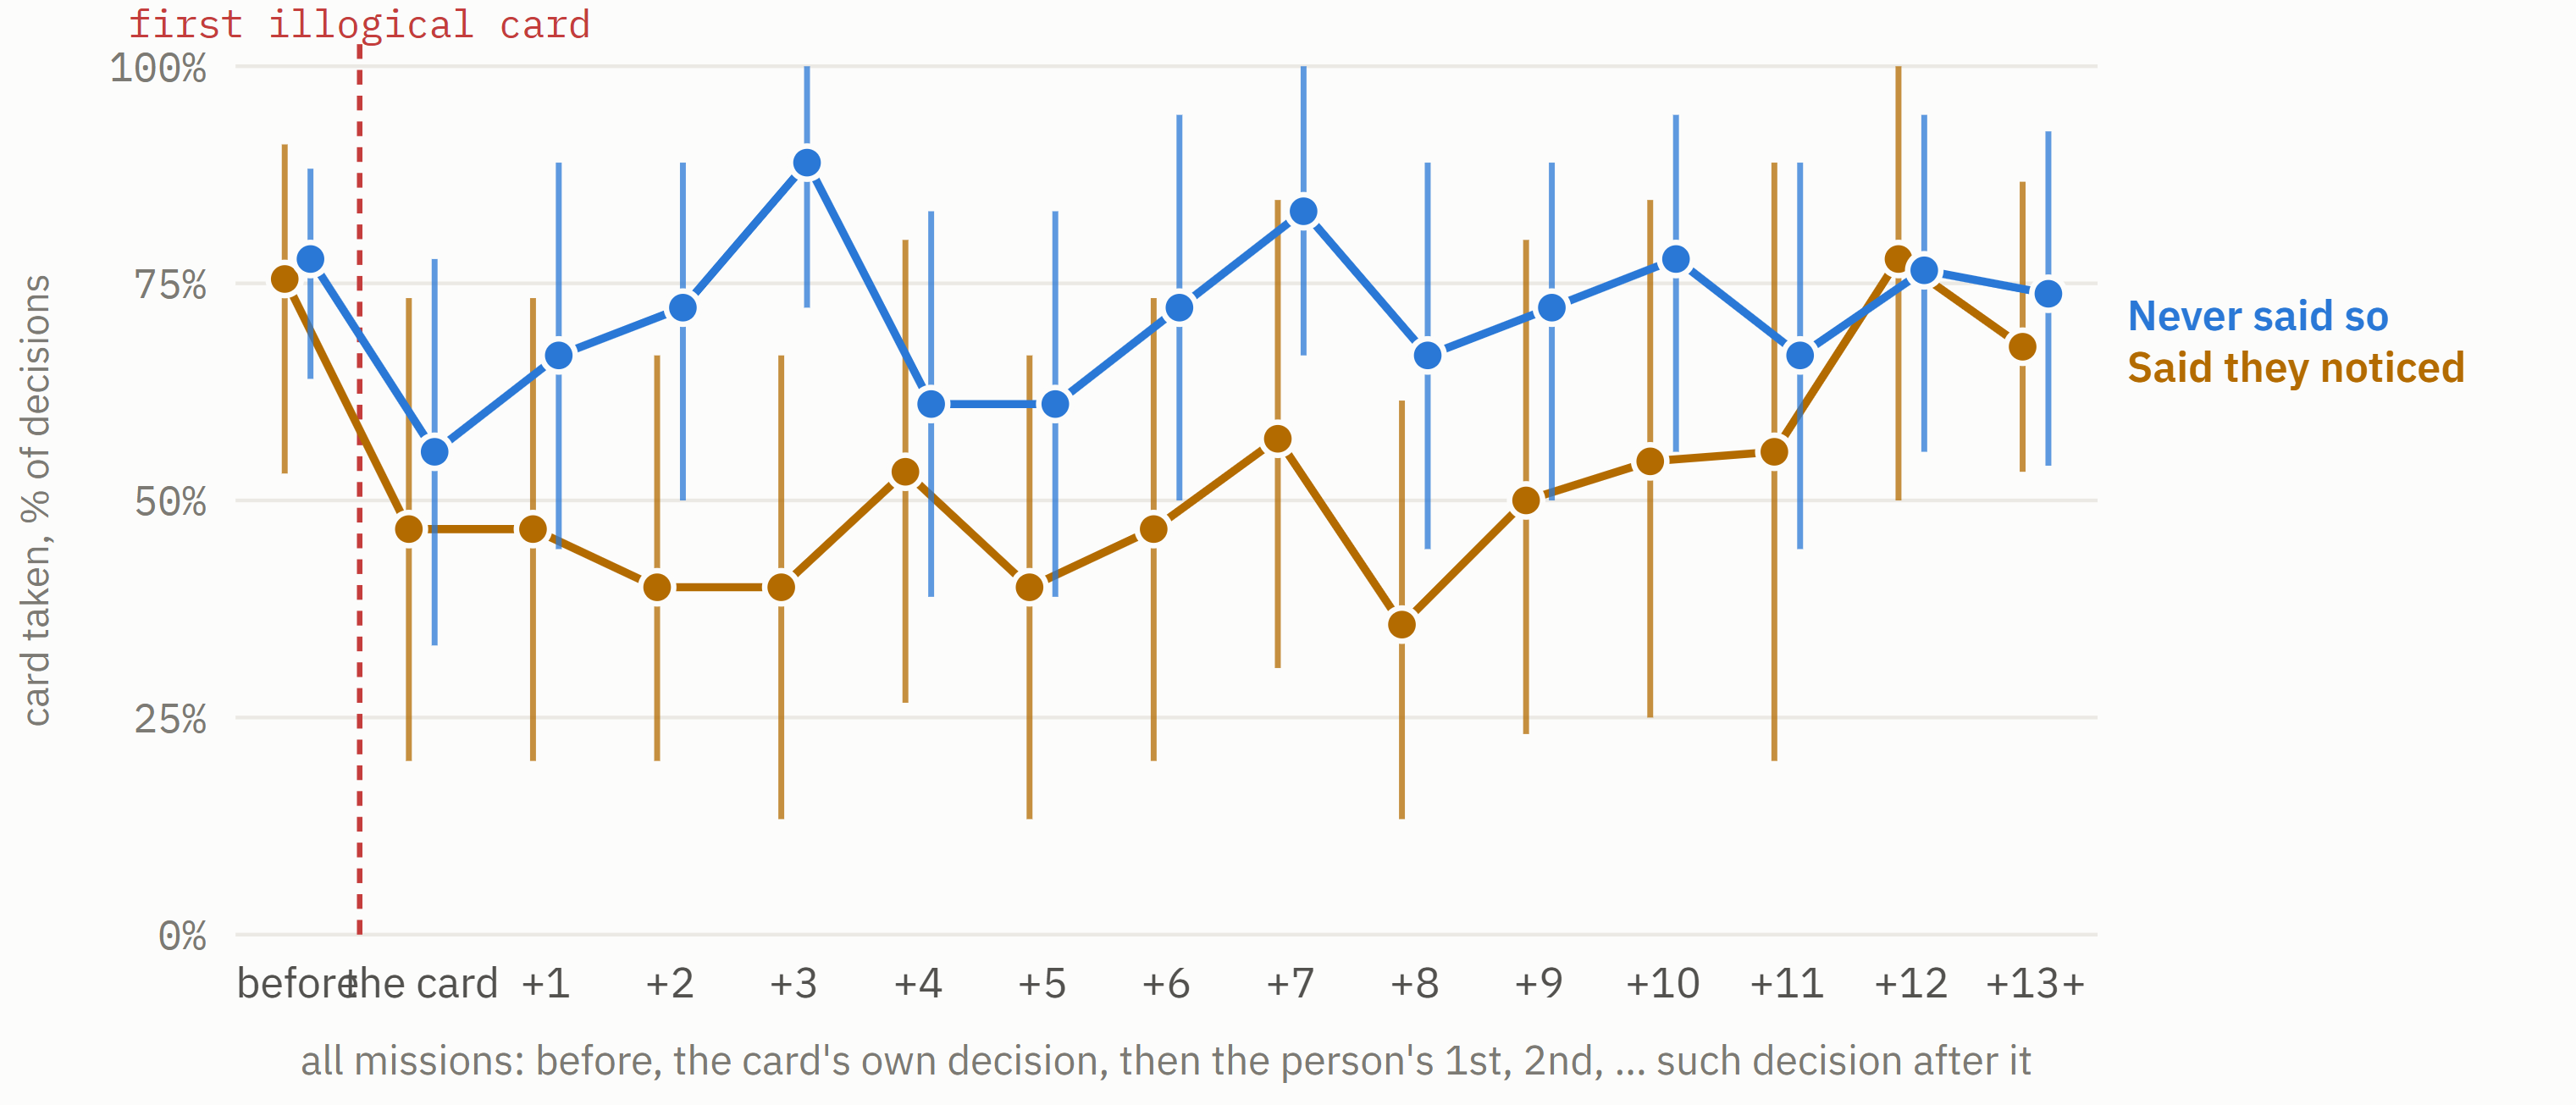
\includegraphics[width=\linewidth,height=0.23\textheight,keepaspectratio]{figs/results/f-flaw-odd__event__steps.png}
\caption{All missions, every step.}
\label{fig:res:flaw-odd:event:steps}
\end{subfigure}
\par\smallskip
\caption{\textbf{The event study, aligned on the first illogical card (every step, pairs or threes)}}
\label{fig:res:flaw-odd:event}
\end{figure}

\paragraph*{Key numbers.}

\begin{itemize}[leftmargin=1.2em,itemsep=1pt]

\item All missions, noticers (15): 76\% before (n 53) $\rightarrow$ card 47\% (n 15) $\rightarrow$ pairs +1--2 to +9--10: 43\%, 47\%, 43\%, 46\%, 52\% $\rightarrow$ 67\% (+11--12) $\rightarrow$ 68\% (13th+, n 31)

\item All missions, never said (18): 78\% before (n 54) $\rightarrow$ 56\% at the card $\rightarrow$ 67--75\% for every later pair

\item All missions, before $\rightarrow$ after, adjusted: noticers $-$14 points, p = .08; never said +9, p = .14; difference $-$14 [$-$30, +1], p = .06

\item Three-type, noticers by pair: 74\% before (n 51), 43\% (n 30), 59\% (n 29), 62\% (n 24), 63\% (n 19), 75\% (n 12)

\item Why expected is lower for noticers: their own-rate term (take rate on all their other decisions) is 56\% vs 70\%; 79\% of a noticer's decisions come at or after the card, where they took 50\% per person vs 72\% (p = .007); before the card the groups were alike (68\% vs 63\%, p = .71)

\item Mission-only expected (own-rate term set to the average): after the card 68\% noticers vs 69\% never-said; before 80\% vs 81\%

\item Steps before the card, all missions: noticers $\leq$$-$4 87\% (n 23), $-$3 88\% (n 8), $-$2 50\% (n 8), $-$1 64\% (n 14); never-said 82\%, 100\%, 88\%, 56\% (n 22, 8, 8, 16)

\item $-$1 against $-$3/$-$2, the 16 people with three steps (all tactical-heavy-first): adjusted $-$13 points [$-$40, +13], p = .29

\item Matched view (8 noticers with 3+ steps, 6 of whom met the card at the start of session 2): 87\%, 88\%, 50\%, 63\% before $\rightarrow$ 38\% at the card $\rightarrow$ 31--44\% for the next ten decisions

\end{itemize}

\paragraph*{Method.} {\small Rows: strategic decisions of the 33 people, split into those who said they noticed (debrief or interview code C12, or a strict in-play remark; 15 people) and those who never said so (18). 'Before' and 'after' are relative to the first illogical card. That decision itself is excluded from both windows and shown as its own point ('the card') in the all-missions view. Change = the 'after' coefficient in a linear model of card uptake, with practice (decision number) held fixed and people clustered for the uncertainty. Raw version: uptake \textasciitilde{} after + practice + game. Adjusted version: (observed $-$ expected) \textasciitilde{} after + practice. The interaction asks whether the after-step differs between the groups. Label shuffle: the said/never-said labels were shuffled across people 5,000 times, to see how often a random split of the same people shows as large a difference in their own after-minus-before. Each person counts once in that test, so it is exact. Steps before the card: $-$1 is each person's last decision before it, $-$2 the one before that, and '$\leq$ $-$4' pools everything earlier; the matched view keeps only the 16 people (8 per group) with at least three such decisions. Mission-only expected: the same model's prediction with each person's own-rate term set to everyone's average.}

\paragraph*{What participants said.} \regtext{12 of 33 said in the debrief or interview that the strategy cards over-allocated or sent unneeded types (C12), and 12 commented on it during play (7 strictly about a card sending an unneeded type). The first sight is often puzzlement rather than a verdict ('unless I'm missing something', 'do fast drones have a higher chance of failing?'), and some took the card anyway (P04) or noticed only after taking it (P20, P29). Dissent: P10 decided the redundancy was sensible; P27 was not sure it was a fault.}

\paragraph*{Quotes selected for this section.}

\begin{quotelist}

\item ``Oh, this just sends a bunch of extra of these even though it doesn't need it?''\,---\,P19 (think-aloud s2 0:36)

\item ``Why is it that the green ones, there's no green or red, unless I'm missing something.''\,---\,P17 (think-aloud s1 5:25)

\item ``And then when it came to assigning them, I noticed, oh, okay, it's made a mistake.''\,---\,P20 (debrief 0:26:11)

\item ``where we can go conservative, but we don't need any, in this one we don't need any lifter or cameras.''\,---\,P30 (think-aloud s1 1:01)

\item ``But I find that the first task it allocated too much Lifter and Camera. So I think I'm less confident for it.''\,---\,P35 (think-aloud s1 1:22)

\item ``there was one example in the first round where it was required all fast drones. And I think the AI assistant recommended I add some red and green drones.''\,---\,P20 (debrief 0:25:51)

\item ``I mean, it was giving me the wrong type of drones. It required only blue drones and kept giving me red and green ones.''\,---\,P21 (debrief 0:35:03)

\item ``But in conservative, you don't need camera or lifters, yet it adds it as reserve. Even for tasks it doesn't do. That doesn't make sense.''\,---\,P13 (debrief 0:29:55)

\item ``deploy a conservative strategy for that one doesn't make sense, I don't think. Because I don't need any red or blue drones.''\,---\,P20 (think-aloud s1 3:41)

\end{quotelist}

\clearpage

\subsubsection{Card use through the session, noticers and never-said}\label{sec:res:flaw-odd:over-time}

\noindent \passtag{for the paper}

\noindent \regtext{\textbf{What is plotted.} Every strategic decision is placed in the minute of the session when its strategy panel opened (0--1 is the first minute). Each point is the share of the decisions in that minute where the person took one of the two strategy cards instead of allocating by hand, with a 95\% band. Nothing is lined up on the illogical card; the small ticks on the axis show when each person first met it. By default it shows \textbf{each group and everyone pooled} (dashed line). \textbf{Session 1}: noticers start at 86\% in the first minute, fall to 50\%, 50\% and 38\% over minutes 1--4, and come back to 73\% in minute 4--5. Never-said people rise over the same minutes, 65\% $\rightarrow$ 88\%. Everyone pooled sits between the two and stays at 61--77\%: the two groups move in opposite directions, so lumping them together hides the dip. That is the point of this chart. \textbf{Session 2}: noticers are lower throughout (52--53\% in the first three minutes, 38\% in minutes 3--5, then 55--73\%); never-said people sit between 61\% and 89\%. Each minute holds 10--30 decisions per group, so single minutes have wide bands: the shape, not any one point, is the result.} (Figure~\ref{fig:res:flaw-odd:over-time})

\begin{figure}[H]
\centering
\begin{subfigure}[t]{\linewidth}
\centering
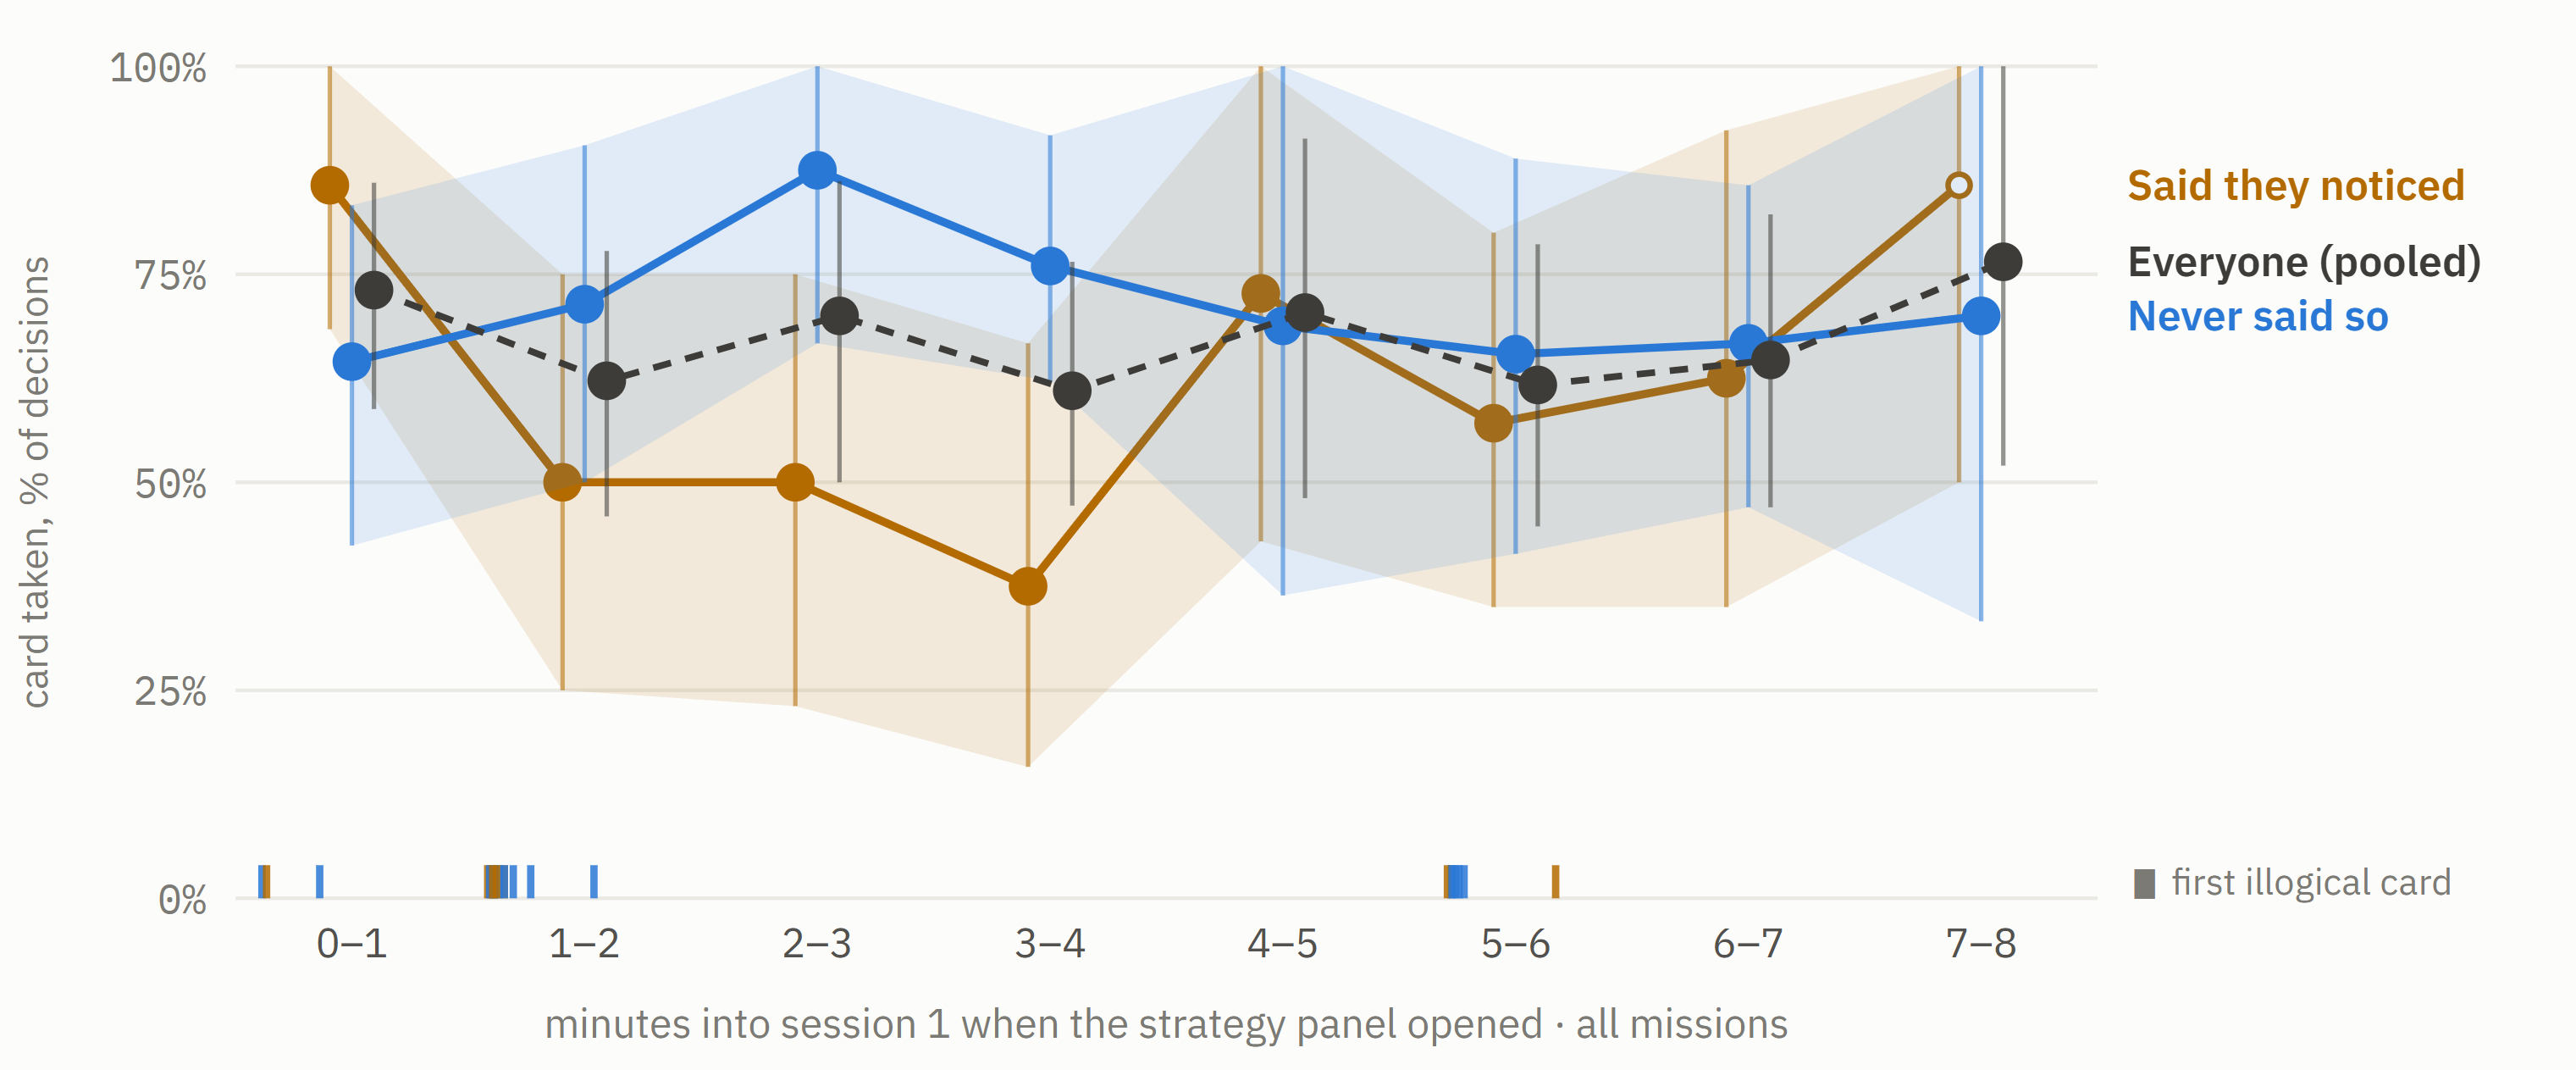
\includegraphics[width=\linewidth,height=0.23\textheight,keepaspectratio]{figs/results/f-flaw-odd__over-time__s1.png}
\caption{Session 1: each group and everyone.}
\label{fig:res:flaw-odd:over-time:s1}
\end{subfigure}
\par\smallskip
\begin{subfigure}[t]{\linewidth}
\centering
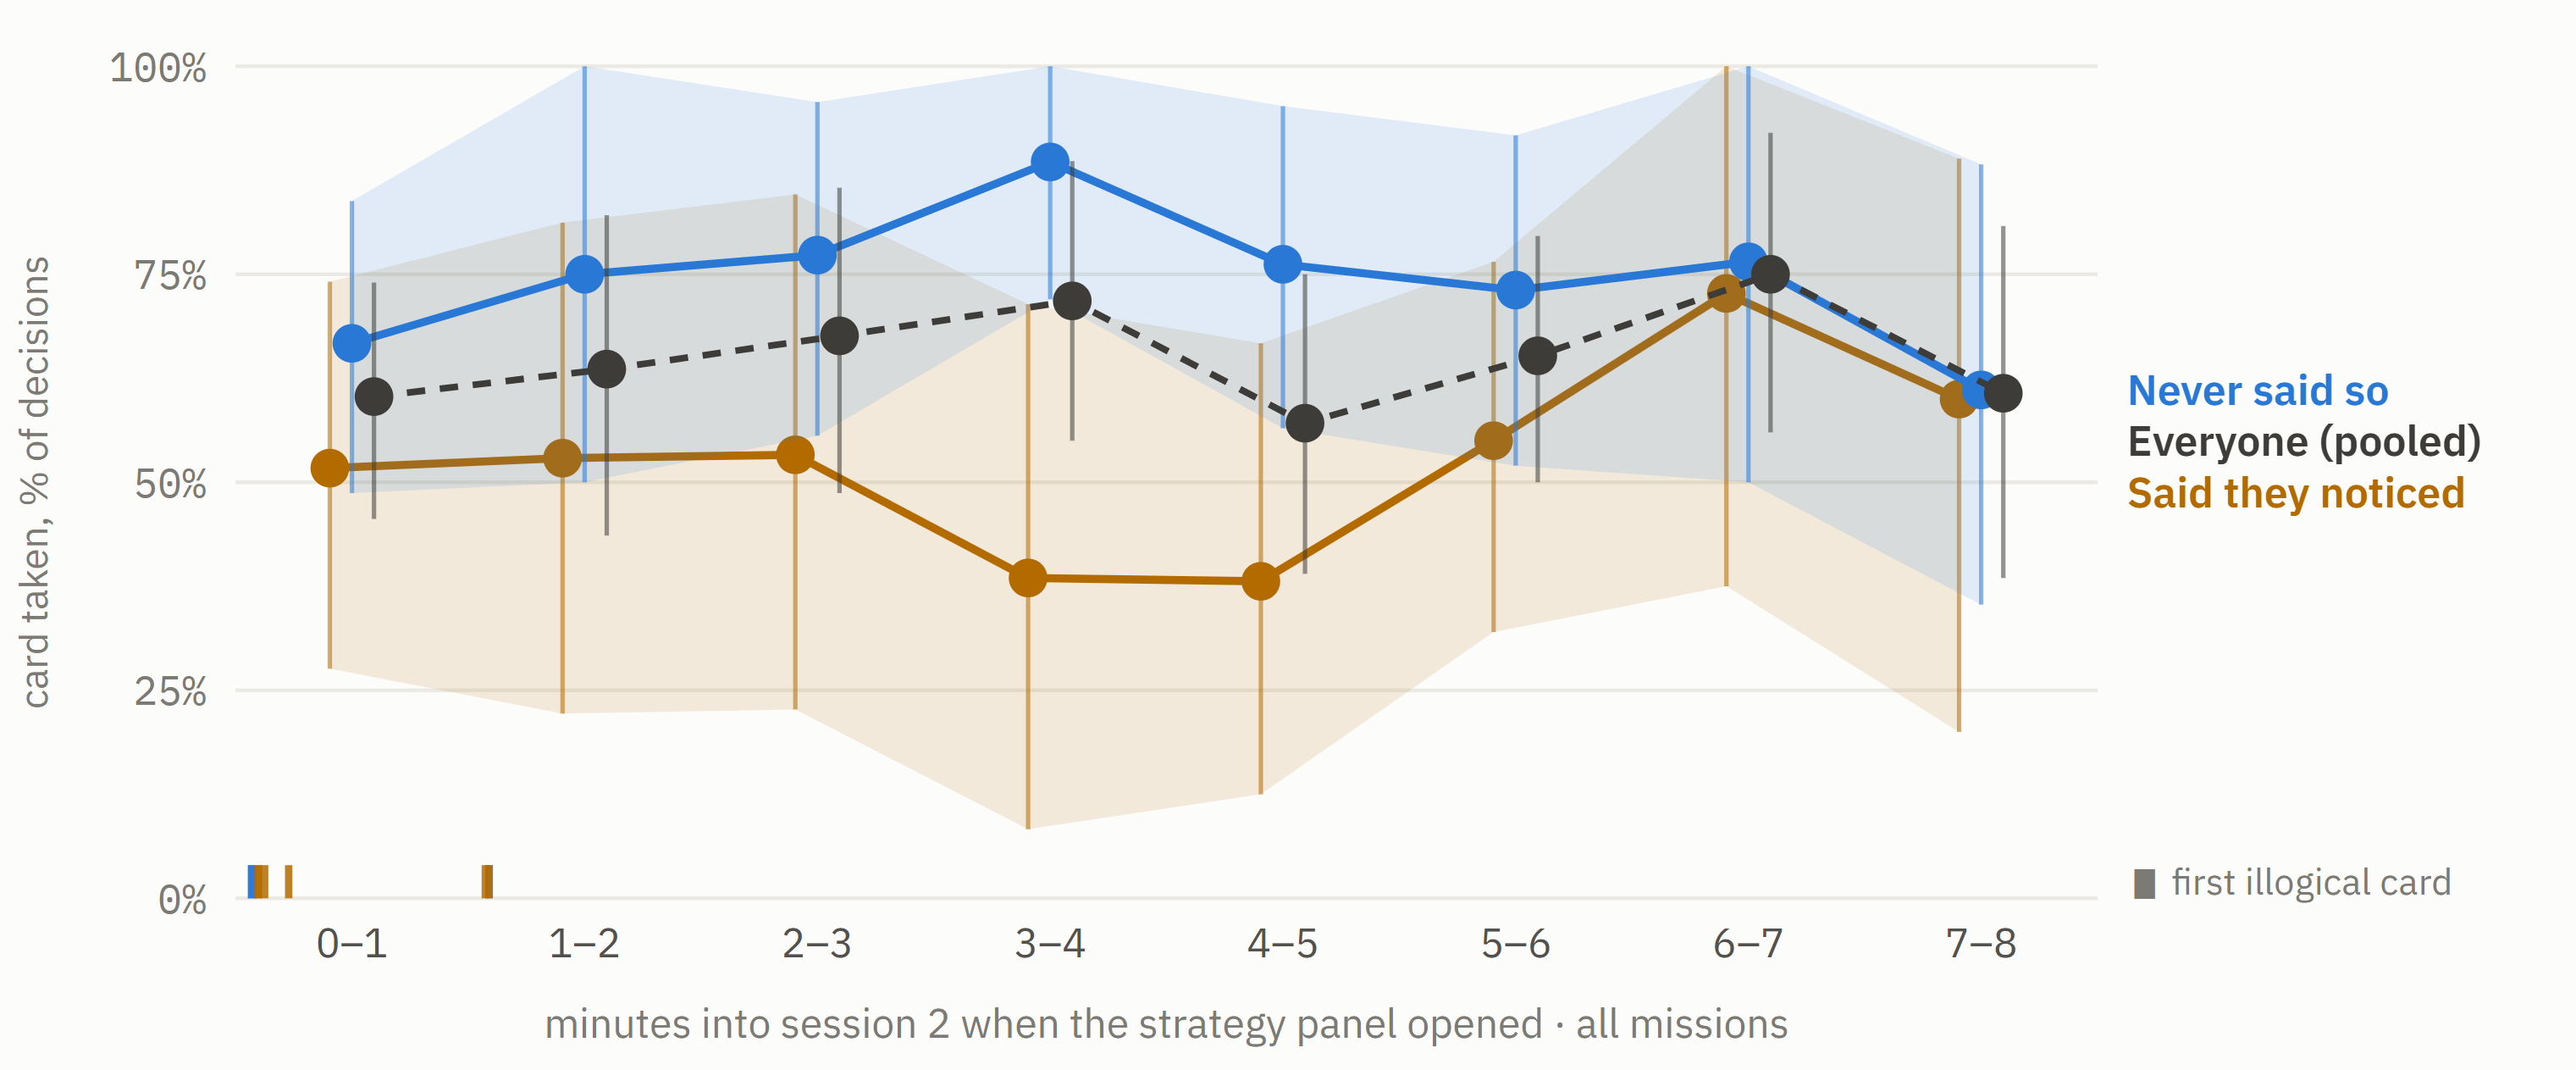
\includegraphics[width=\linewidth,height=0.23\textheight,keepaspectratio]{figs/results/f-flaw-odd__over-time__s2.png}
\caption{Session 2: each group and everyone.}
\label{fig:res:flaw-odd:over-time:s2}
\end{subfigure}
\par\smallskip
\caption{\textbf{Card use through the session, noticers and never-said}}
\label{fig:res:flaw-odd:over-time}
\end{figure}

\paragraph*{Key numbers.}

\begin{itemize}[leftmargin=1.2em,itemsep=1pt]

\item Session 1, noticers by minute 0--1 to 4--5: 86\% (n 21), 50\% (n 16), 50\% (n 14), 38\% (n 16), 73\% (n 11)

\item Session 1, never said: 65\% (n 31), 71\%, 88\%, 76\%, 69\%

\item Session 2, noticers: 52\% (n 29), 53\%, 53\%, 38\% (n 13), 38\% (n 21), 55\%, 73\%, 60\%; never said 61--89\%

\end{itemize}

\paragraph*{Method.} {\small Rows: every strategic decision, binned by the minute of the session at which its panel opened (the last bin, 7--8 min, is thin). Rate = share of decisions where a card was taken; 95\% bands from resampling people. Adjusted = the group's overall rate plus the mean of (observed $-$ expected) from the adjustment model, i.e. relative to each person's own habit given the mission in front of them. Game order: strategic-heavy-first players met the illogical card at about 67 s of session 1; 7 tactical-heavy-first players at about 315 s, the other 9 at the very start of session 2.}

\paragraph*{What participants said.} \regtext{Nobody describes a dip-and-recover in their own words, but the pieces are there: several noticed early in session 1 (P35 in the first two minutes, P13 at minute 3, P20 at minute 4) and went manual for a while, and those who say why they kept using the cards give speed --- it is less reliable 'but at least it saves time' (P28). P20, asked if their trust was destroyed: 'No. Definitely not\ldots{} most of the time it seemed accurate'.}

\paragraph*{Quotes selected for this section.}

\begin{quotelist}

\item ``I think it's less reliable than before, but I still use its suggestion, and that's the case. Yeah, because at least it saves time.''\,---\,P28 (debrief 0:29:56)

\item ``I know there is a better choice, but I have no time to tune everything.''\,---\,P28 (debrief 0:30:33)

\end{quotelist}

\clearpage

\subsubsection{Card use by decision number, session 1 then session 2, not aligned to the card}\label{sec:res:flaw-odd:by-index}

\noindent \passtag{for the paper}

\noindent \regtext{Each person's decisions are numbered in the order they made them within each session (or counting only three-type, one/two-type, or missions with no illogical card). \textbf{Session 1 and session 2 sit on one axis}, separated by a dashed line, with the two sessions' lines deliberately not joined (session 2 is a different game, after a break and a survey). \textbf{Later numbers are different people}: only those who made that many decisions reach them, and they are mostly players of the strategic-heavy game, which has more missions. So a point is drawn only if at least 8 people of its group reach it; dot size and the numbers under the axis show how many people each point rests on. \textbf{Session 1}: noticers 80\%, 67\%, 47\%, 50\%, 46\%, then 83\%, 64\%, 78\% for decisions 6--8; never-said 61\%, 61\%, 78\%, 94\%, 89\%, 72\%. Noticers dip at 3--5 and climb back (+24 points per person). The same shape holds in a fixed panel of the 9 noticers and 12 never-said people who made at least 8 decisions (noticers 44\% at decisions 4--5, 78--89\% at 6 and 8), so it is not a change of who is counted. \textbf{Session 2}: noticers 47--53\% for six decisions, then 30--38\% at 7--9; never-said people 61--92\%. The late low is the mission mix: around decisions 7--8 of the strategic-heavy game half the missions show the illogical card, and noticers took it on 17\% of those against 62\% of the rest. Leaving those missions out, noticers and never-said people meet at decisions 7--8 (71\% against 70--73\%). Noticers start session 2 below where they ended session 1 (64\% $\rightarrow$ 49\%), but never-said people also start a little lower (76\% $\rightarrow$ 69\%); the difference at the break is small and uncertain ($-$6 points [$-$32, +20]), and $-$9 [$-$30, +12] for noticers after allowing for the mission mix. The very last numbers of each session (session 1 decisions 9--11+, session 2 decision 10 and 11+ for noticers) rest on 2--6 noticers and are hidden; the \emph{Thin points} button shows them.} (Figure~\ref{fig:res:flaw-odd:by-index})

\begin{figure}[H]
\centering
\begin{subfigure}[t]{\linewidth}
\centering
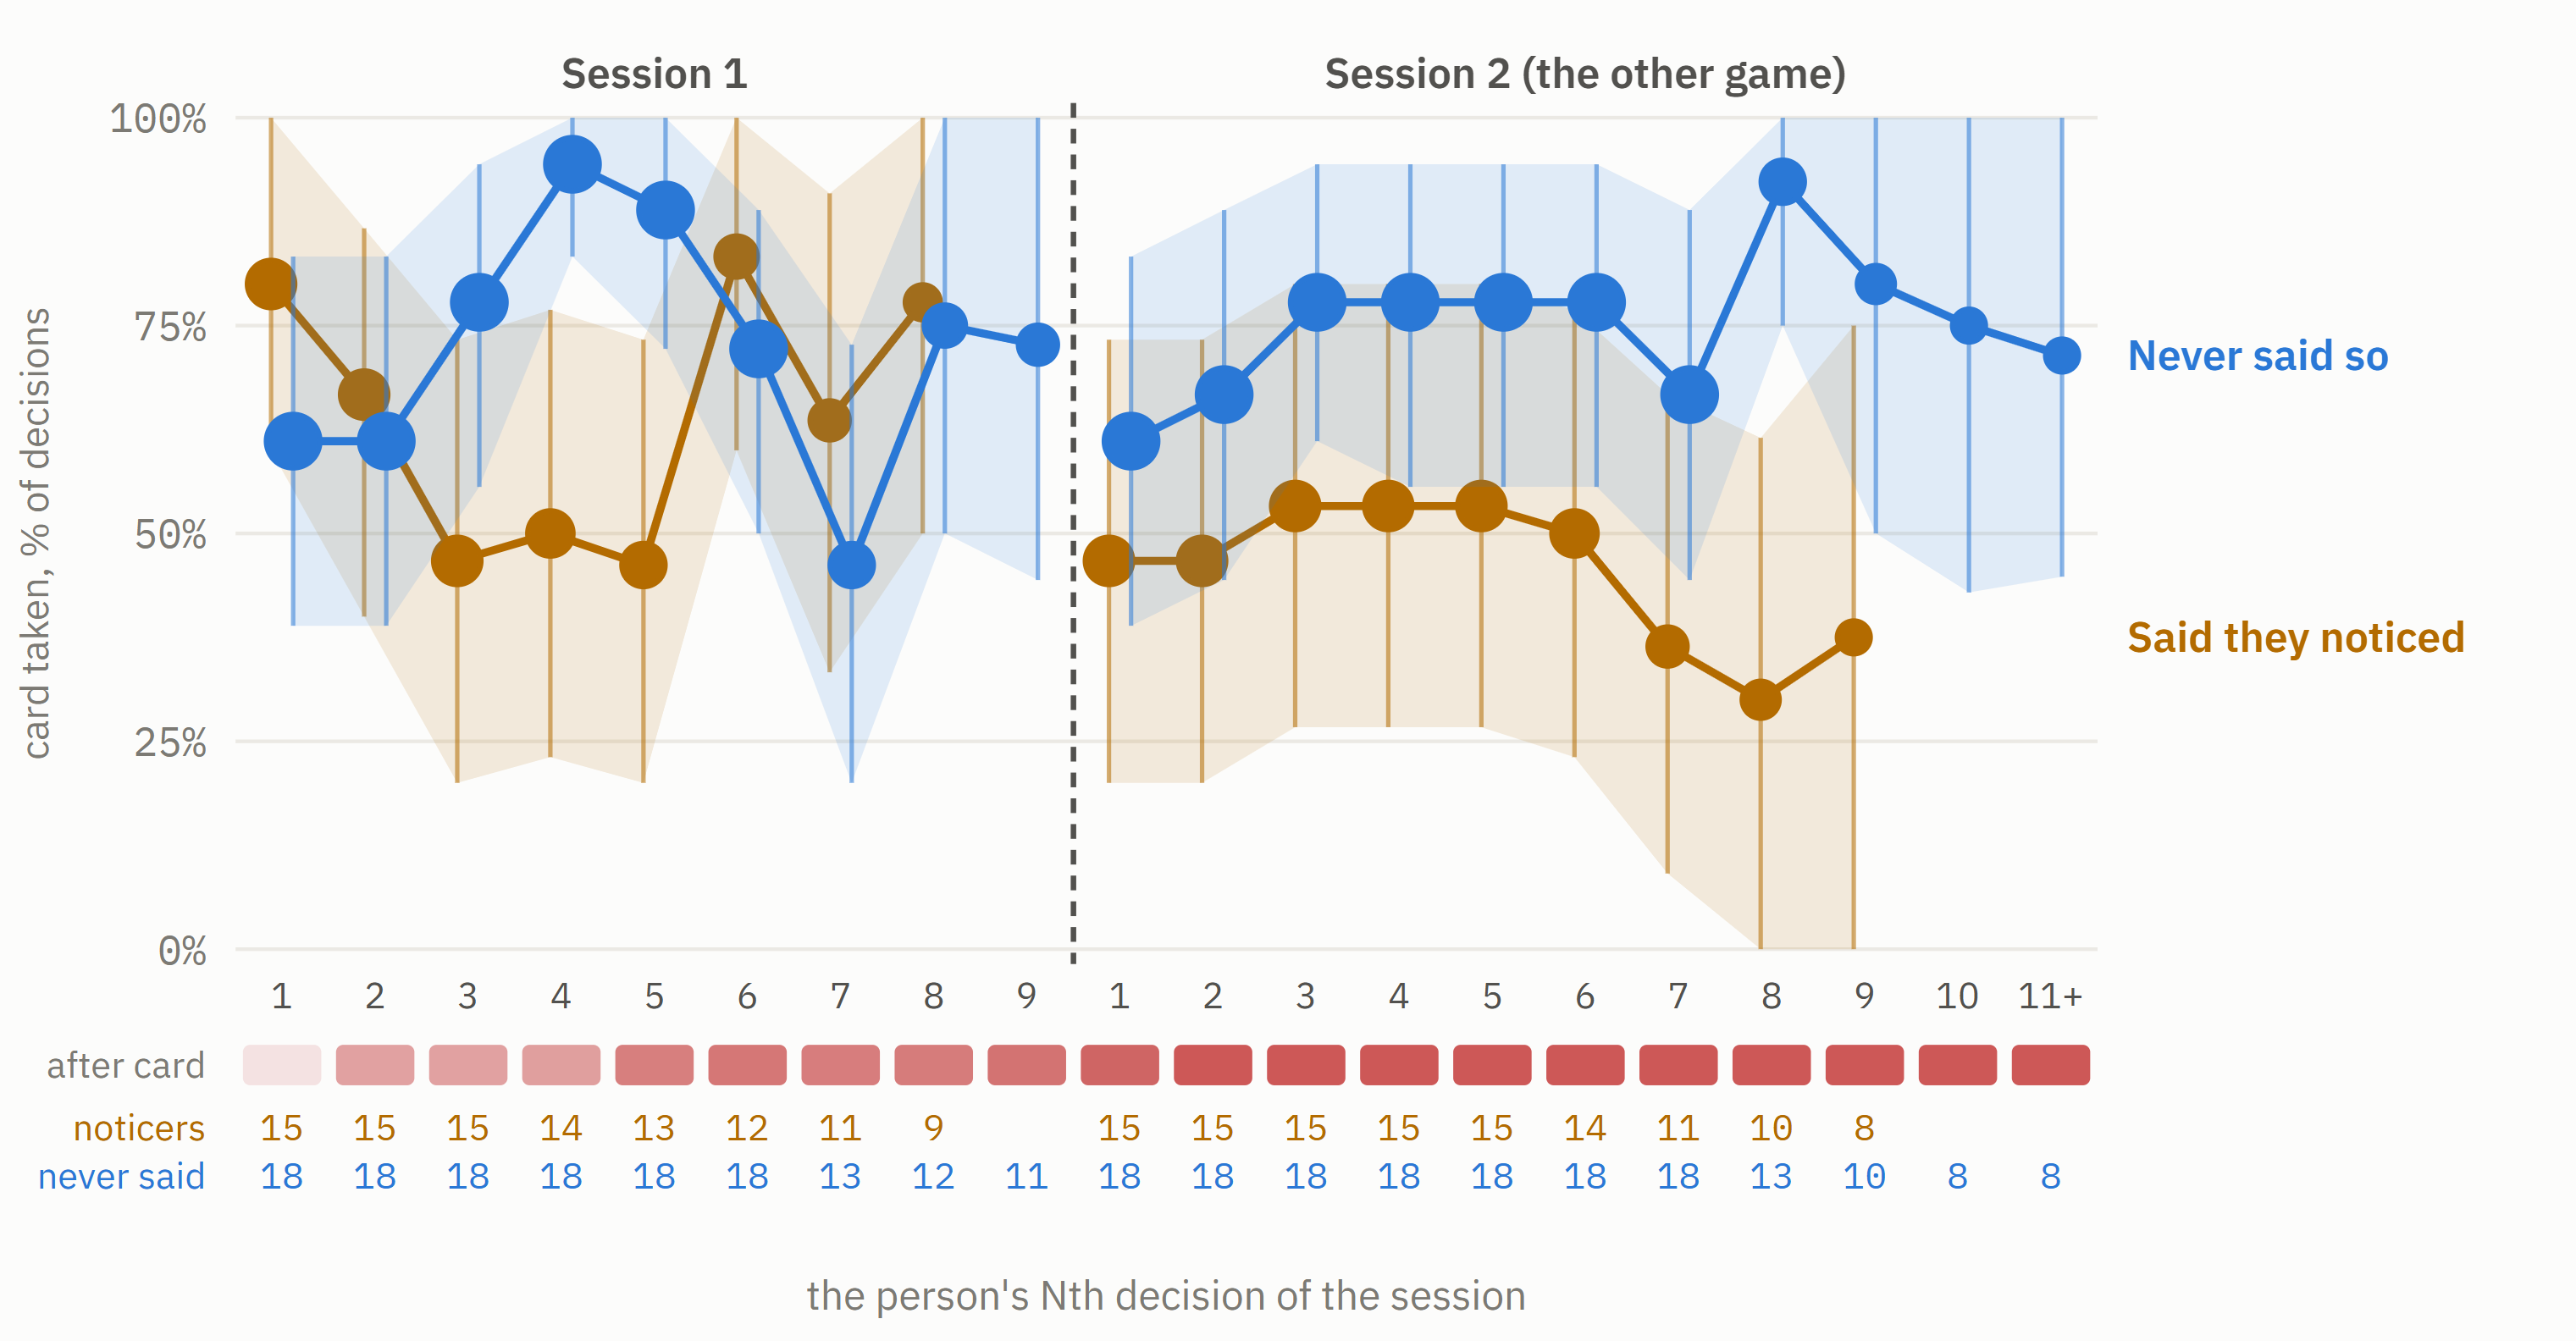
\includegraphics[width=\linewidth,height=0.23\textheight,keepaspectratio]{figs/results/f-flaw-odd__by-index__groups.png}
\caption{Noticers against never-said, session 1 then session 2.}
\label{fig:res:flaw-odd:by-index:groups}
\end{subfigure}
\par\smallskip
\begin{subfigure}[t]{\linewidth}
\centering
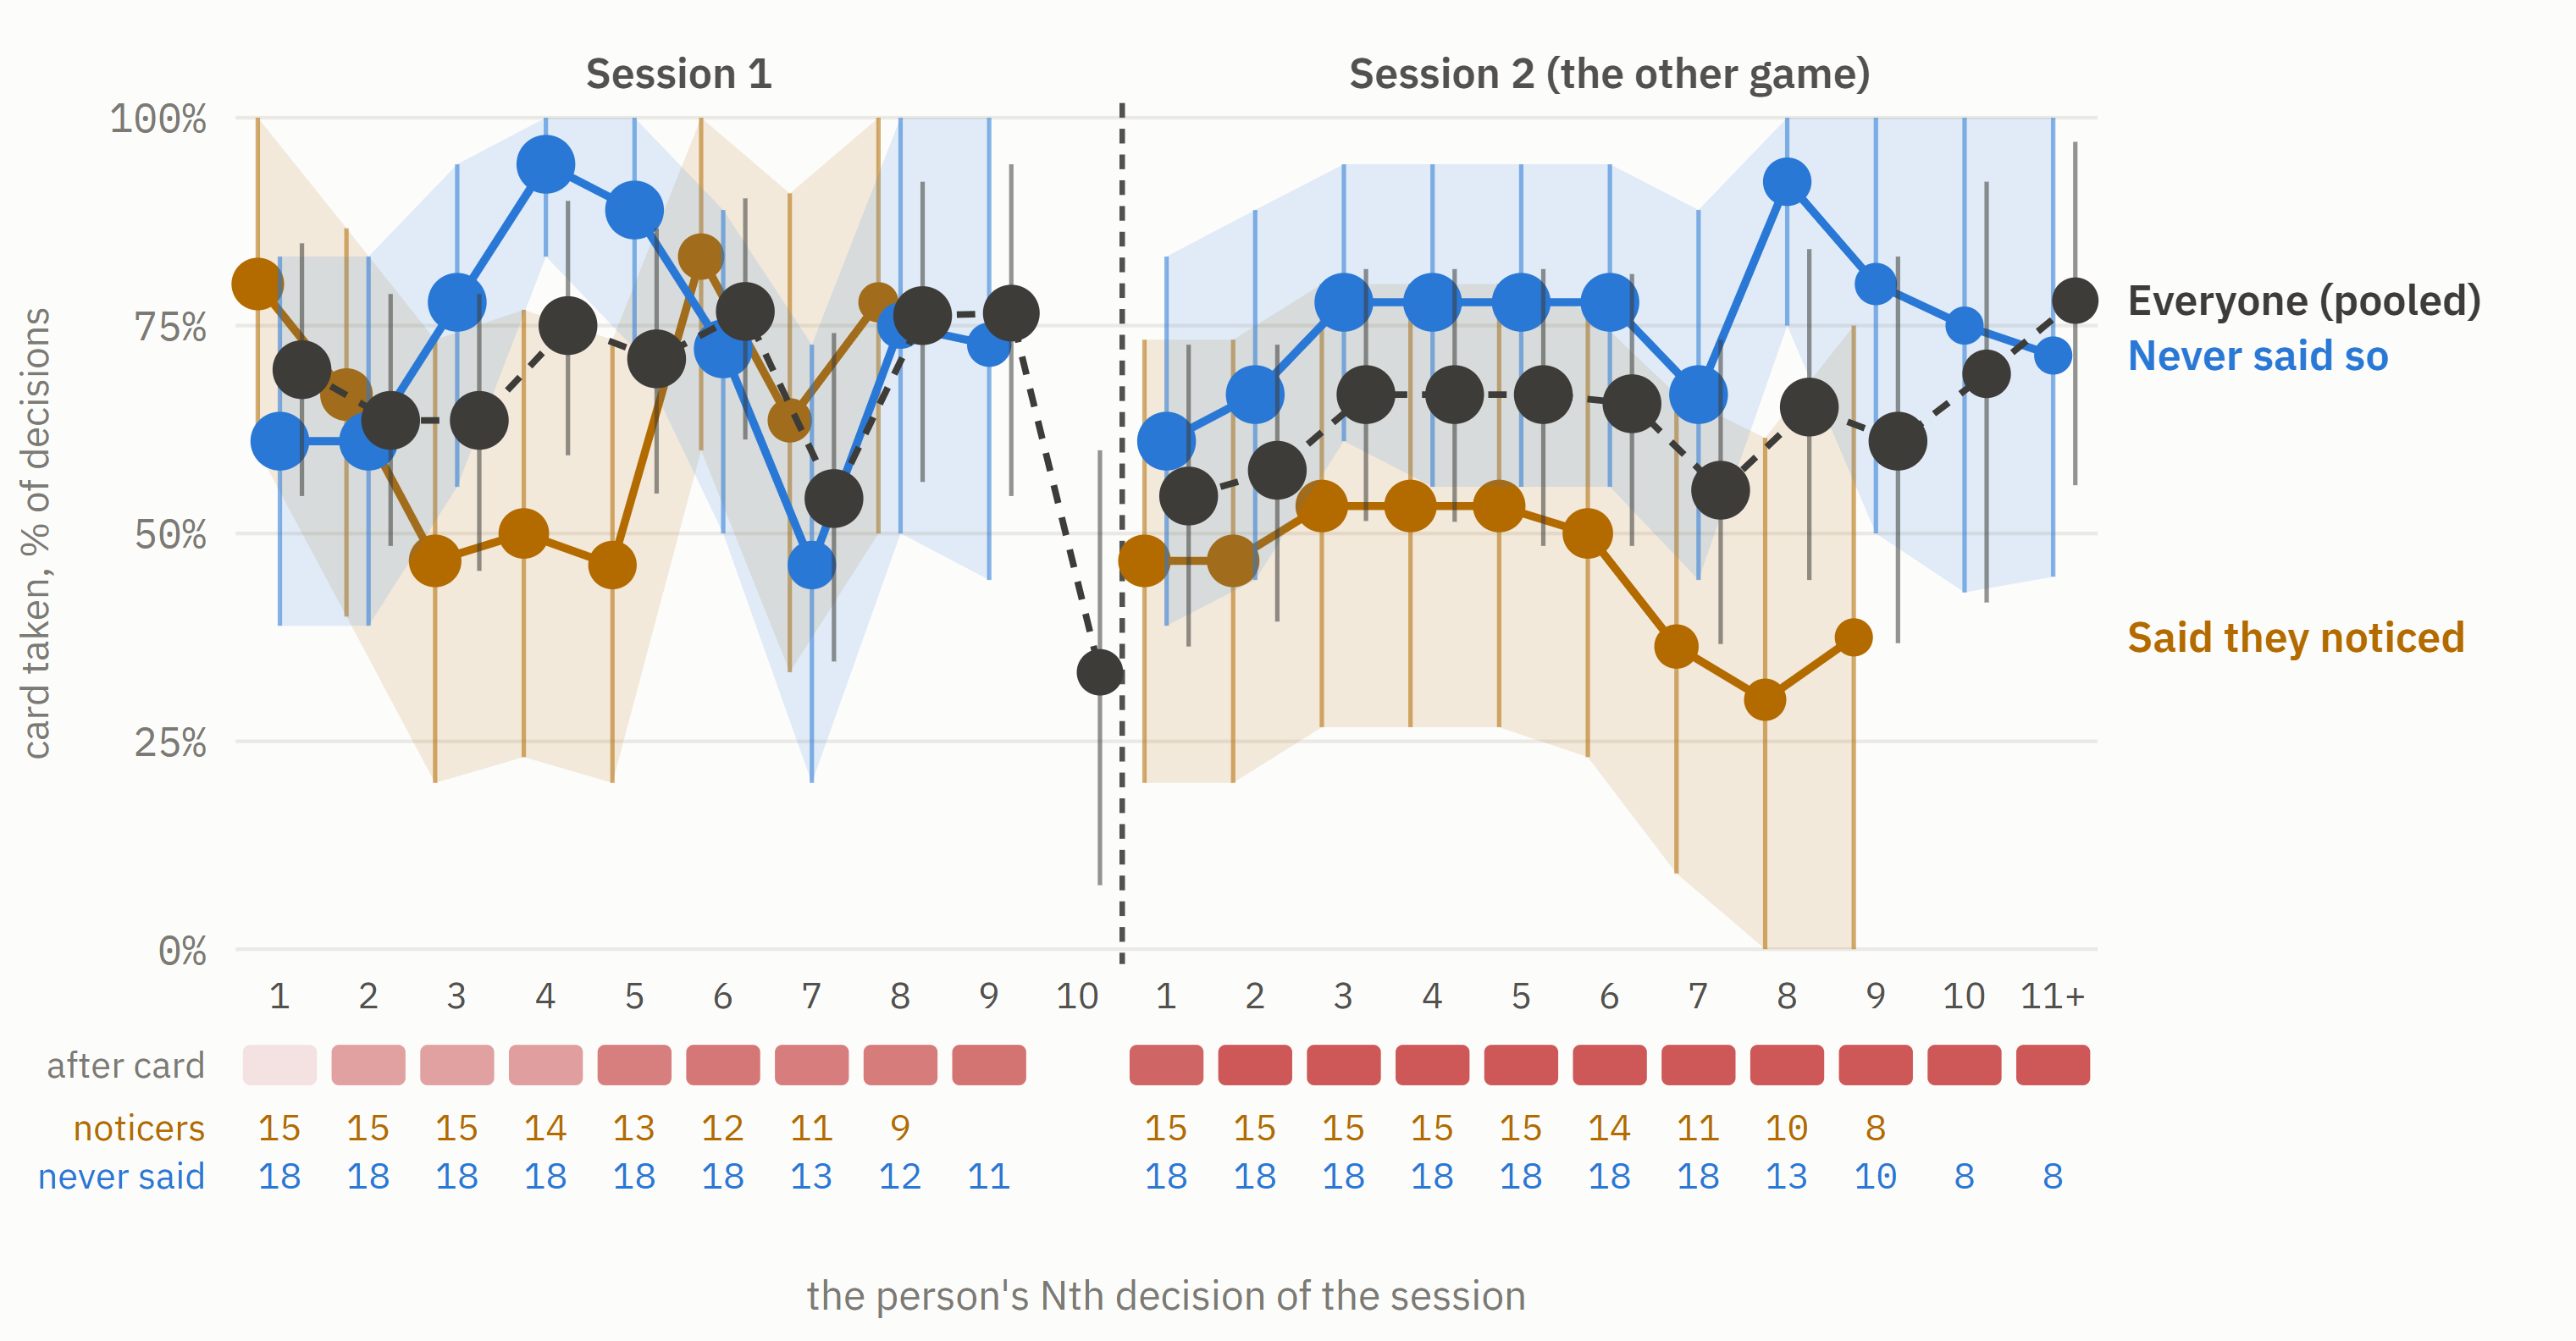
\includegraphics[width=\linewidth,height=0.23\textheight,keepaspectratio]{figs/results/f-flaw-odd__by-index__everyone.png}
\caption{Each group and everyone.}
\label{fig:res:flaw-odd:by-index:everyone}
\end{subfigure}
\par\smallskip
\caption{\textbf{Card use by decision number, session 1 then session 2, not aligned to the card}}
\label{fig:res:flaw-odd:by-index}
\end{figure}

\paragraph*{Key numbers.}

\begin{itemize}[leftmargin=1.2em,itemsep=1pt]

\item Everyone, session 1, decisions 1--6: 70\%, 64\%, 64\%, 75\%, 71\%, 77\% (n 33 $\rightarrow$ 30)

\item Noticers, session 1: 80\%, 67\%, 47\%, 50\%, 46\%, 83\%, 64\%, 78\% (decisions 1--8, 15 $\rightarrow$ 9 people); never said: 61\%, 61\%, 78\%, 94\%, 89\%, 72\%, 46\%, 75\%, 73\% (decisions 1--9, 18 $\rightarrow$ 11 people)

\item Session 1 fixed panel (9 noticers, 12 never-said, decisions 1--8): noticers 78, 67, 56, 44, 44, 89, 56, 78\%; never said 50, 42, 67, 92, 83, 67, 50, 75\%

\item Session 1 tail (hidden): decision 9, 6 noticers 83\%; decision 10, 5 noticers 1 of 5 took (20\% [4, 62]), 7 never-said 43\% [16, 75]; 11+, 2 noticers 3 of 7 (one took 3 of 4, the other 0 of 3), 5 never-said 7 of 12. All strategic-heavy-game players; 57--67\% of the 11+ decisions in the last 90 s

\item Session 2 tail (hidden for noticers): decision 10, 5 noticers 60\%; 11+, 4 noticers (all tactical-heavy first, so playing the strategic-heavy game) 12 of 13 = 92\% [67, 99], against 8 never-said 20 of 28 = 71\%. These 4 took cards on 42\% of their decisions 1--6, below their group's 51\%: not keen takers surviving

\item Strategic-heavy game: share of decisions with an illogical card at decisions 7, 8, 9, 10, 11+: 48\%, 55\%, 30\%, 4\%, 5\%. At decisions 7+, noticers took 17\% of illogical-card missions (n 18, 9 people) and 62\% of the rest (n 53); never-said 68\% and 69\%

\item Session 2, no illogical card: noticers 71\% at decisions 7 and 8 (7 people) against never-said 73\% and 70\%; earlier the gap is there (decisions 2--3: 33--47\% against 67--89\%)

\item Session 2 fixed panel (8 noticers, 10 never-said, decisions 1--9): gap over the last 3 decisions $-$47 points [$-$81, $-$12] against $-$19 [$-$50, +12] before; on missions with no illogical card (panel to decision 6) $-$17 [$-$45, +12] against $-$30 [$-$61, +1]

\item At the session break (last 3 of session 1 $\rightarrow$ first 3 of session 2): noticers 64\% $\rightarrow$ 49\%, $-$16 points [$-$38, +4], p = .17; adjusted $-$9 [$-$30, +12]; never-said 76\% $\rightarrow$ 69\%, $-$7 [$-$24, +7]; difference $-$6 [$-$32, +20], p = .66

\item Recovery within session 1 (decisions 3--5 $\rightarrow$ 6+): noticers 48\% (n 42) $\rightarrow$ 66\% (n 50), +24 points per person [+5, +43], p = .04 (window read off the curve, so descriptive)

\end{itemize}

\paragraph*{Method.} {\small Rows: every strategic decision; position = its rank among that person's decisions of the chosen kind in that session (positions past 10 pooled as 11+). Rate = share where a card was taken, 95\% bands from resampling people, n decisions and people in each tooltip, with the point's share of three-type missions, illogical-card missions, strategic-heavy-game decisions and last-90-s decisions. \textbf{Minimum}: a point is drawn by default only if at least 8 people of its group (both game orders together) reach that number, about half of the smaller group. \textbf{Fixed panel}: per session and mission kind, K = the largest number that at least 8 people in each group reach; only people with at least K decisions, decisions 1--K (all missions: session 1 K = 8, 9 noticers and 12 never-said; session 2 K = 9, 8 and 10). 'No illogical card' drops the decisions on missions whose Conservative card showed an unused drone type, then renumbers. 'After card' strip = share of the position's decisions made at or after the person's first illogical card. Carry-over checks, per person then averaged (intervals from resampling people, p from a t-test over people): (a) recovery = the rest of session 1 (decisions 6+) minus decisions 3--5; (b) break = the first three decisions of session 2 minus the last three of session 1; (c) start-to-start. Group differences = the interaction in a linear model with people clustered; adjusted versions use observed $-$ expected.}

\paragraph*{What participants said.} \regtext{4 of 33 said they caught the assistant's mistakes more, or were more careful, in the second session (C15: P15, P17, P19, P33), and P15 and P33 add that in the first session there was no time to check. One said the opposite: P20 saw no strategic issues in the second run. No one connects it to which game they played.}

\clearpage

\subsubsection{Lined up on the moment they said a strategy card was wrong: card use falls (7 people, a direction only)}\label{sec:res:flaw-odd:spoken}

\noindent \passtag{for the paper}

\noindent \regtext{\emph{This section is about noticing the strategy card's flaw; the next section is a different event (the Tactical Assistant failing to offer a recovery plan), so the two are not in conflict.} Here each person is anchored on the moment they said, during play, that a card was wrong. Seven people made a strict remark (a card sends types the mission does not need, or a specific card is wrong); five more made broader 'too many drones' remarks. For four of the seven, an illogical card was on screen as they spoke. P30's remark was about an illogical card that opened 5 s later, so it was moved onto that card. P29 spoke 28 s after taking the illogical card. P04's remark was about too many drones on a three-type card. The chart pools each set of people, before vs after the remark, with \textbf{all missions and one- and two-type missions side by side}. On all missions the seven went from 80\% to 49\% (adjusted $-$21 points [$-$49, +7], p = .11, timing-matched placebo p = .51; five fell and two rose). On one- and two-type missions, the ones that carry the illogical card, the drop is larger, 83\% $\rightarrow$ 35\%, but that 'before' bar is only 6 decisions from 4 people, so it is a direction, not a measured size. Seven people cannot settle it; the direction matches the main result.} (Figure~\ref{fig:res:flaw-odd:spoken})

\begin{figure}[H]
\centering
\begin{subfigure}[t]{\linewidth}
\centering
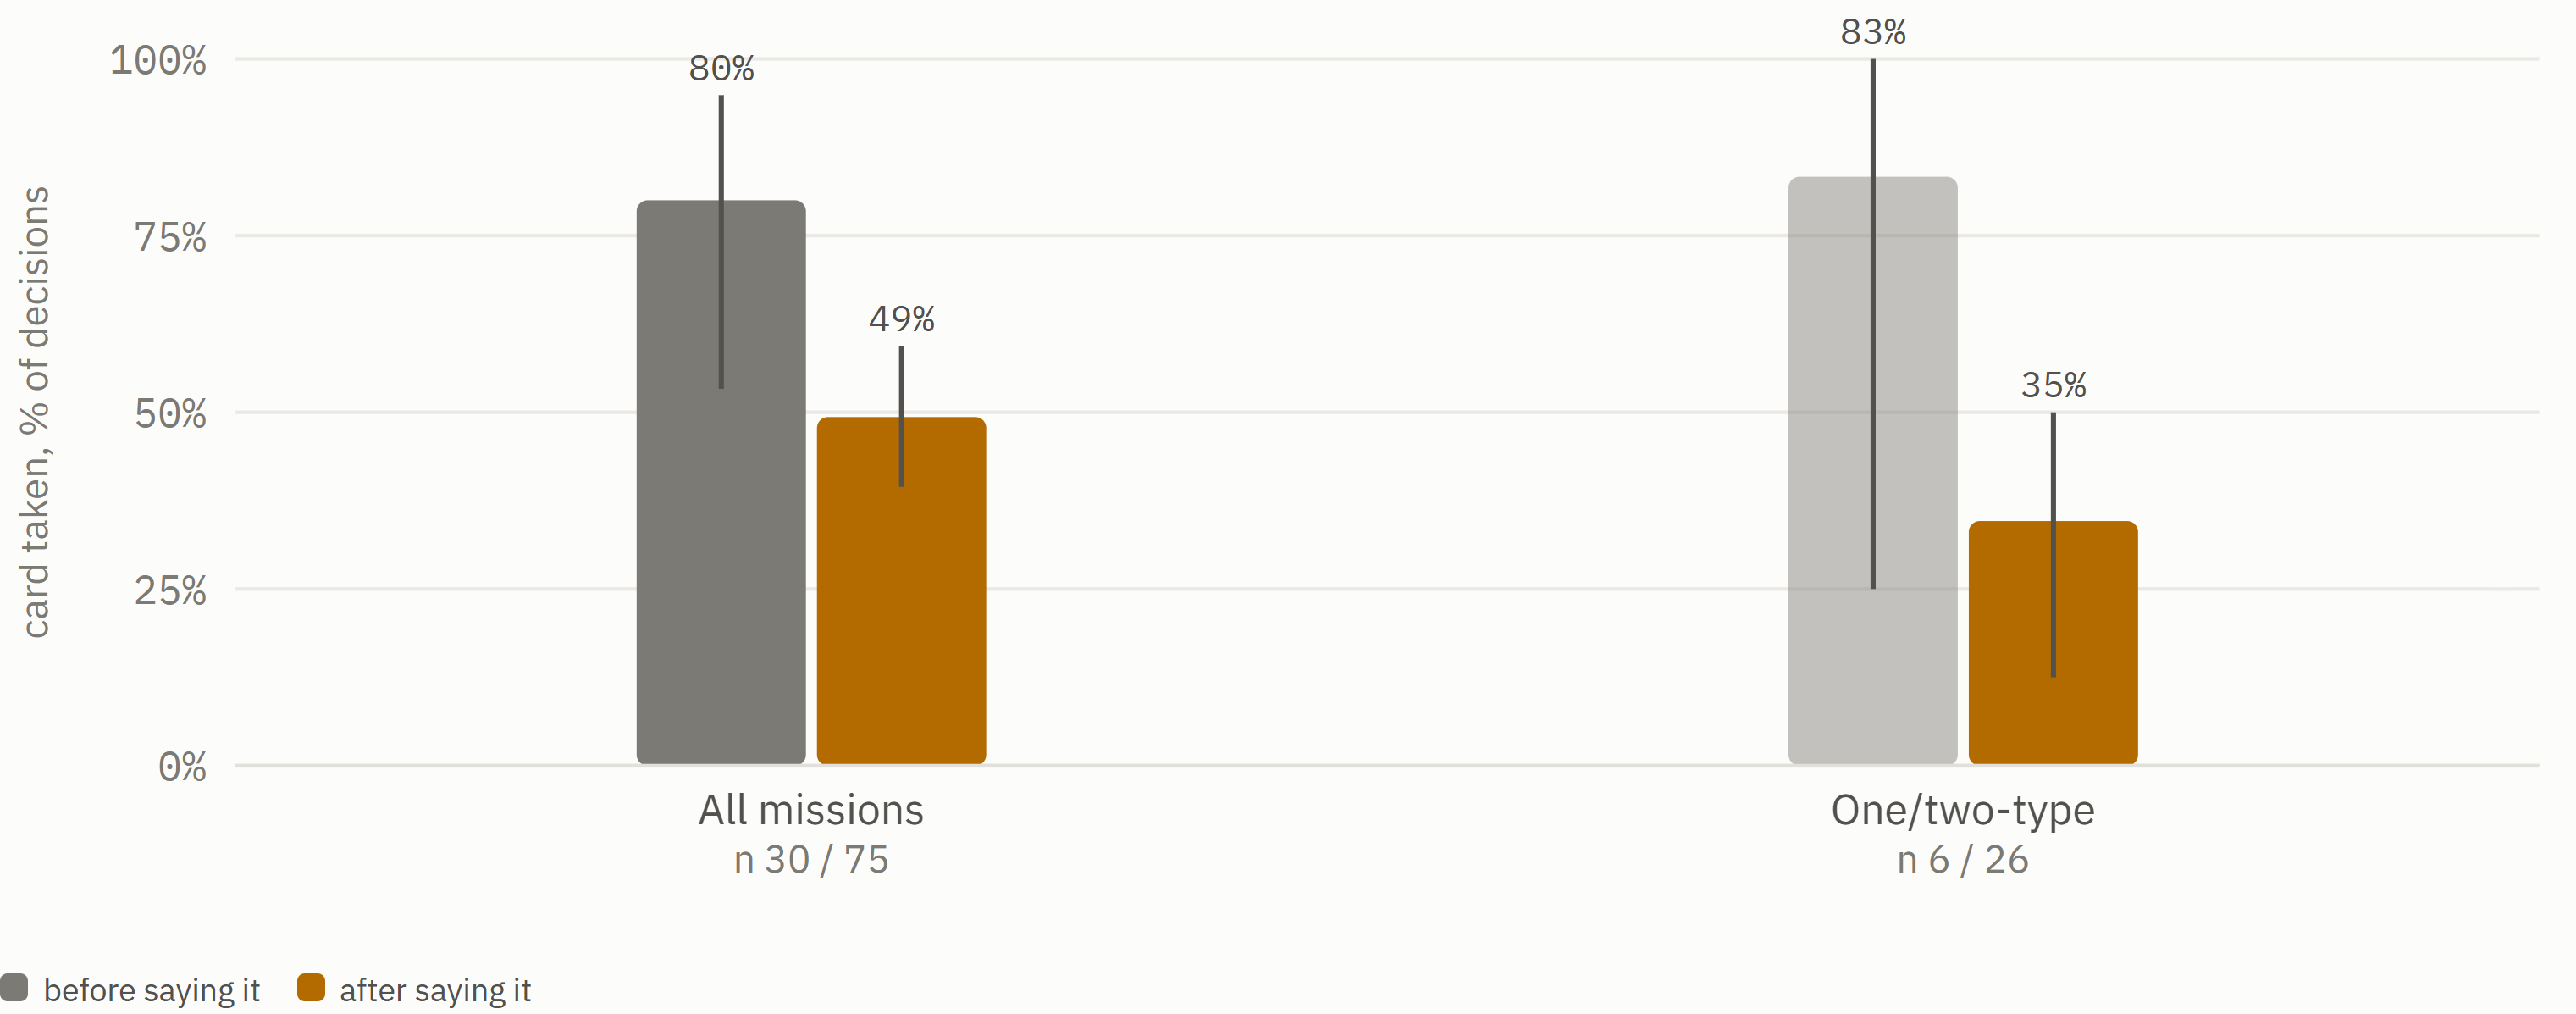
\includegraphics[width=\linewidth,height=0.23\textheight,keepaspectratio]{figs/results/f-flaw-odd__spoken__strict.png}
\caption{Strict remarks: all missions against one- and two-type missions.}
\label{fig:res:flaw-odd:spoken:strict}
\end{subfigure}
\par\smallskip
\begin{subfigure}[t]{\linewidth}
\centering
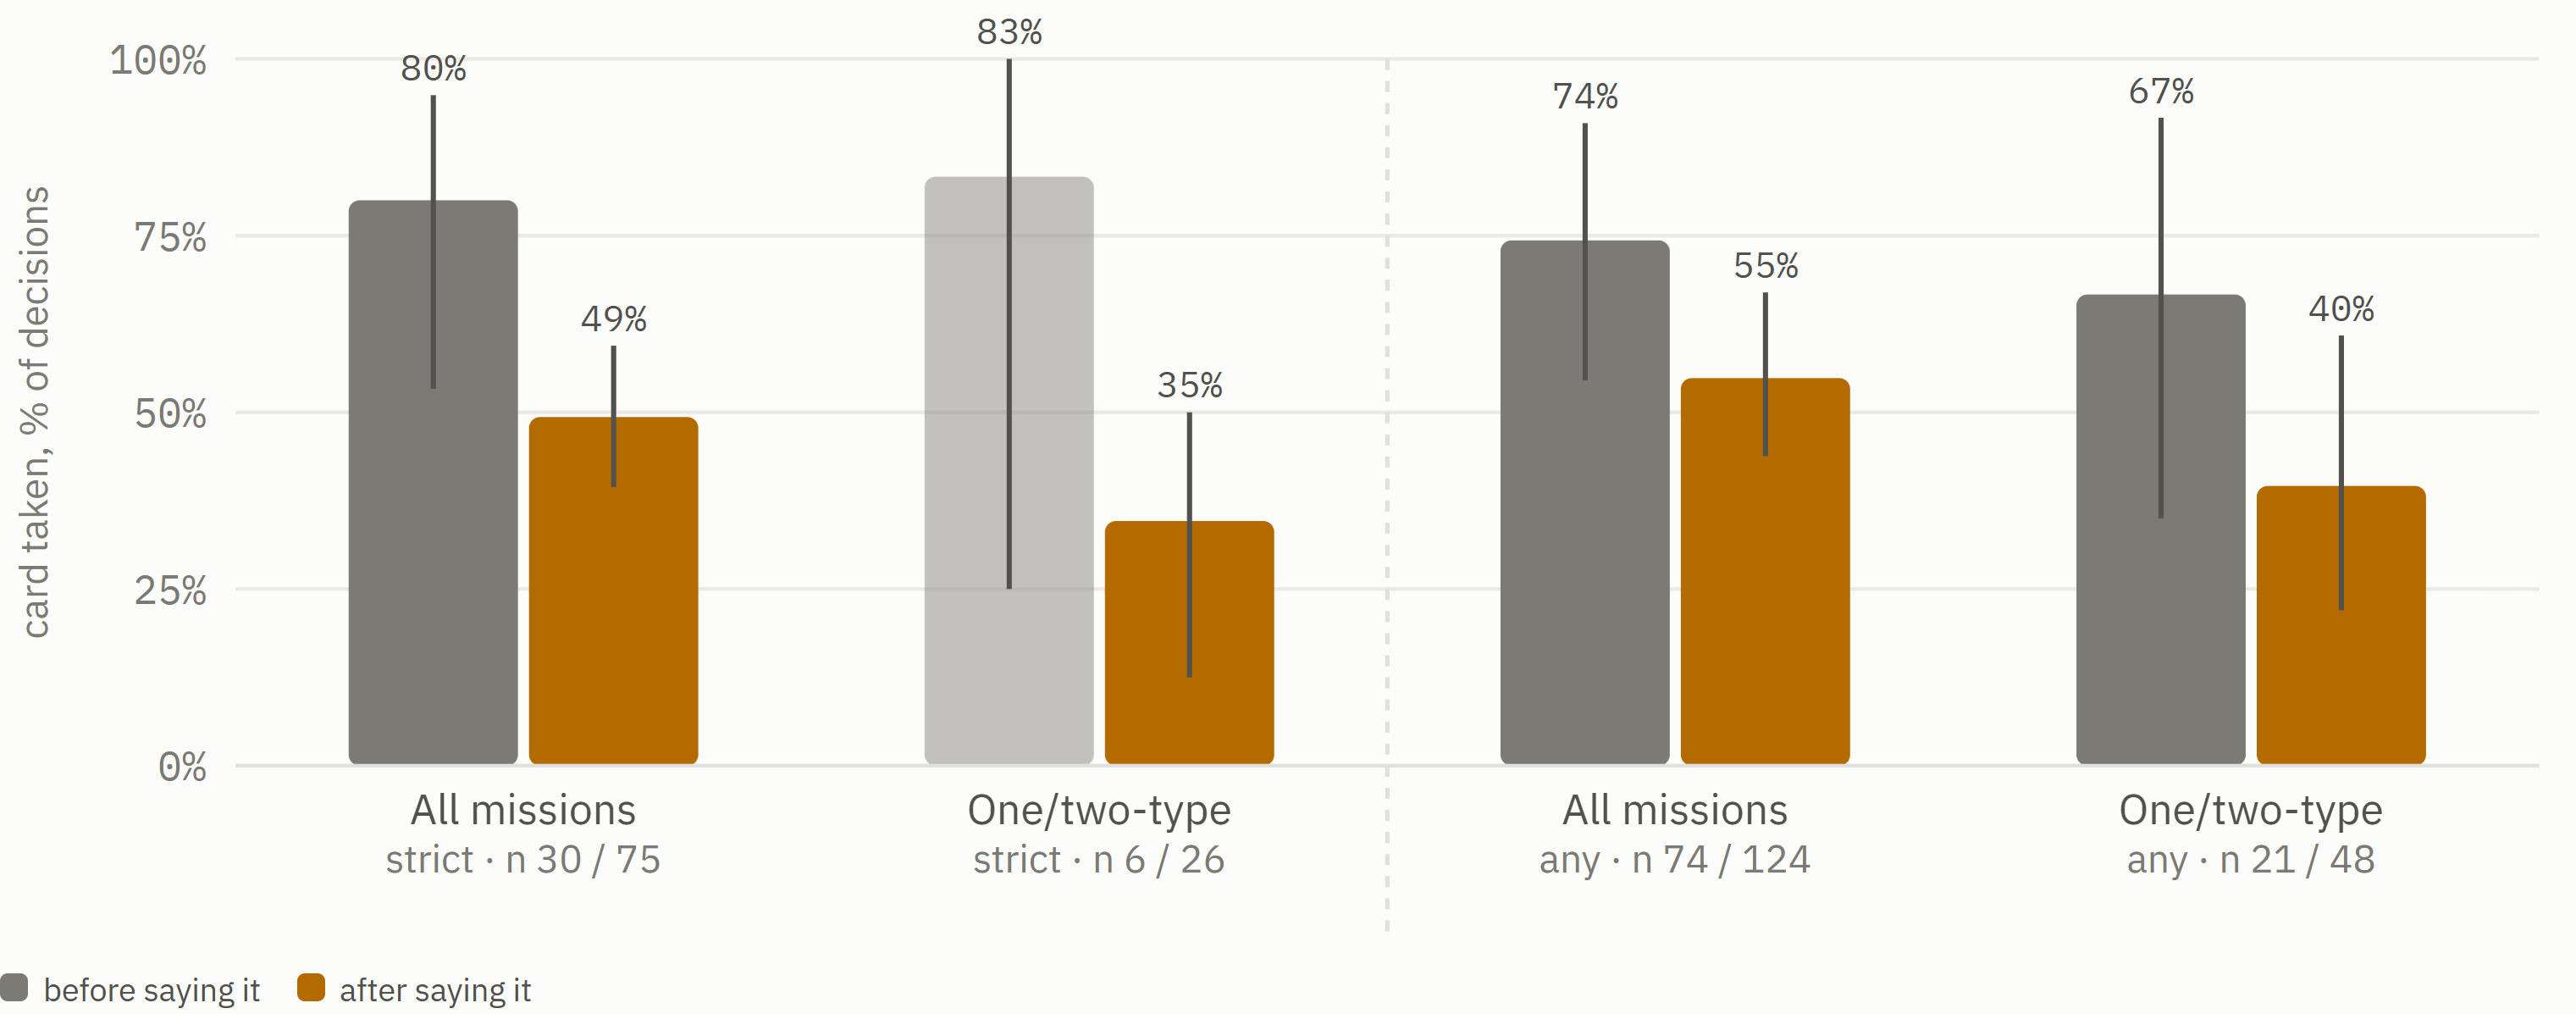
\includegraphics[width=\linewidth,height=0.23\textheight,keepaspectratio]{figs/results/f-flaw-odd__spoken__any.png}
\caption{Strict and any remark, side by side.}
\label{fig:res:flaw-odd:spoken:any}
\end{subfigure}
\par\smallskip
\caption{\textbf{Lined up on the moment they said a strategy card was wrong: card use falls (7 people, a direction only)}}
\label{fig:res:flaw-odd:spoken}
\end{figure}

\paragraph*{Key numbers.}

\begin{itemize}[leftmargin=1.2em,itemsep=1pt]

\item Strict remarks (7 people), all missions: 80\% (n 30) $\rightarrow$ 49\% (n 75); adjusted $-$21 points [$-$49, +7], p = .11; 5 fell, 2 rose; placebo p = .51

\item Strict, one/two-type: 83\% (n 6, 4 people) $\rightarrow$ 35\% (n 26, 7 people); three-type: 79\% (n 24) $\rightarrow$ 57\% (n 49)

\item Any remark (12 people), all missions: 74\% (n 74) $\rightarrow$ 55\% (n 124), adjusted $-$4 points, p = .60; one/two-type 67\% (n 21) $\rightarrow$ 40\% (n 48)

\end{itemize}

\paragraph*{Method.} {\small The spoken moments were hand-coded from the in-play narration before any behaviour around them was computed (extras.SPOKEN\_STRAT, session time). A decision whose card was open at that moment is the anchor decision. Otherwise, 'before' and 'after' are split at the remark. The same models and placebo as above are used.}

\paragraph*{What participants said.} \regtext{The in-play remarks are short and pointed ('It's just wrong', 'You don't need all of that') and are usually followed by going manual (P19, P29, P35, P13), sometimes by taking the card anyway (P04). Four people make further in-play remarks that the anchor list leaves out, late in session 2: P19, P21, P35, and P32. P32 has no C12 code, so they are counted as never having said it, yet they said 'It's just wrong' about an unneeded Camera on a card (s2 5:45).}

\clearpage

\subsubsection{A different event: after the Tactical Assistant's first 'No workable plan', nothing changes on either tier}\label{sec:res:flaw-odd:refusal}

\noindent \passtag{numbers only}

\noindent \regtext{\emph{Not the same moment as the previous section.} Here each person is lined up on the first time the Tactical Assistant's Suggest, asked for a plan to recover from a drone failure, answered 'No workable plan'. That is a failure of the other assistant, and nothing to do with noticing the illogical strategy card. Does \emph{strategic} use go down after the first refusal, with the problem cascading up the chain? \textbf{It does not.} After their first 'No workable plan' (18 people), card uptake actually went \emph{up} in raw terms (68\% $\rightarrow$ 76\%). The expected value went up just as much, because these refusals tend to come later, when people have settled in. Adjusted, the change is +2 points [$-$6, +10], with 10 people falling and 8 rising. On three-type missions it is 0 points. Tactical Suggest use also rose raw (78\% $\rightarrow$ 87\%) and is flat adjusted ($-$1 point). After the first \emph{wrong} refusal (14 people) the picture is the same: strategic $-$2.5 points [$-$16, +11], tactical 0. The first drone failure (33 people) changes nothing either. These are absences of evidence, with intervals around $\pm$10 points. They are not proof of no effect, but no cascade is visible.} (Figure~\ref{fig:res:flaw-odd:refusal})

\begin{figure}[H]
\centering
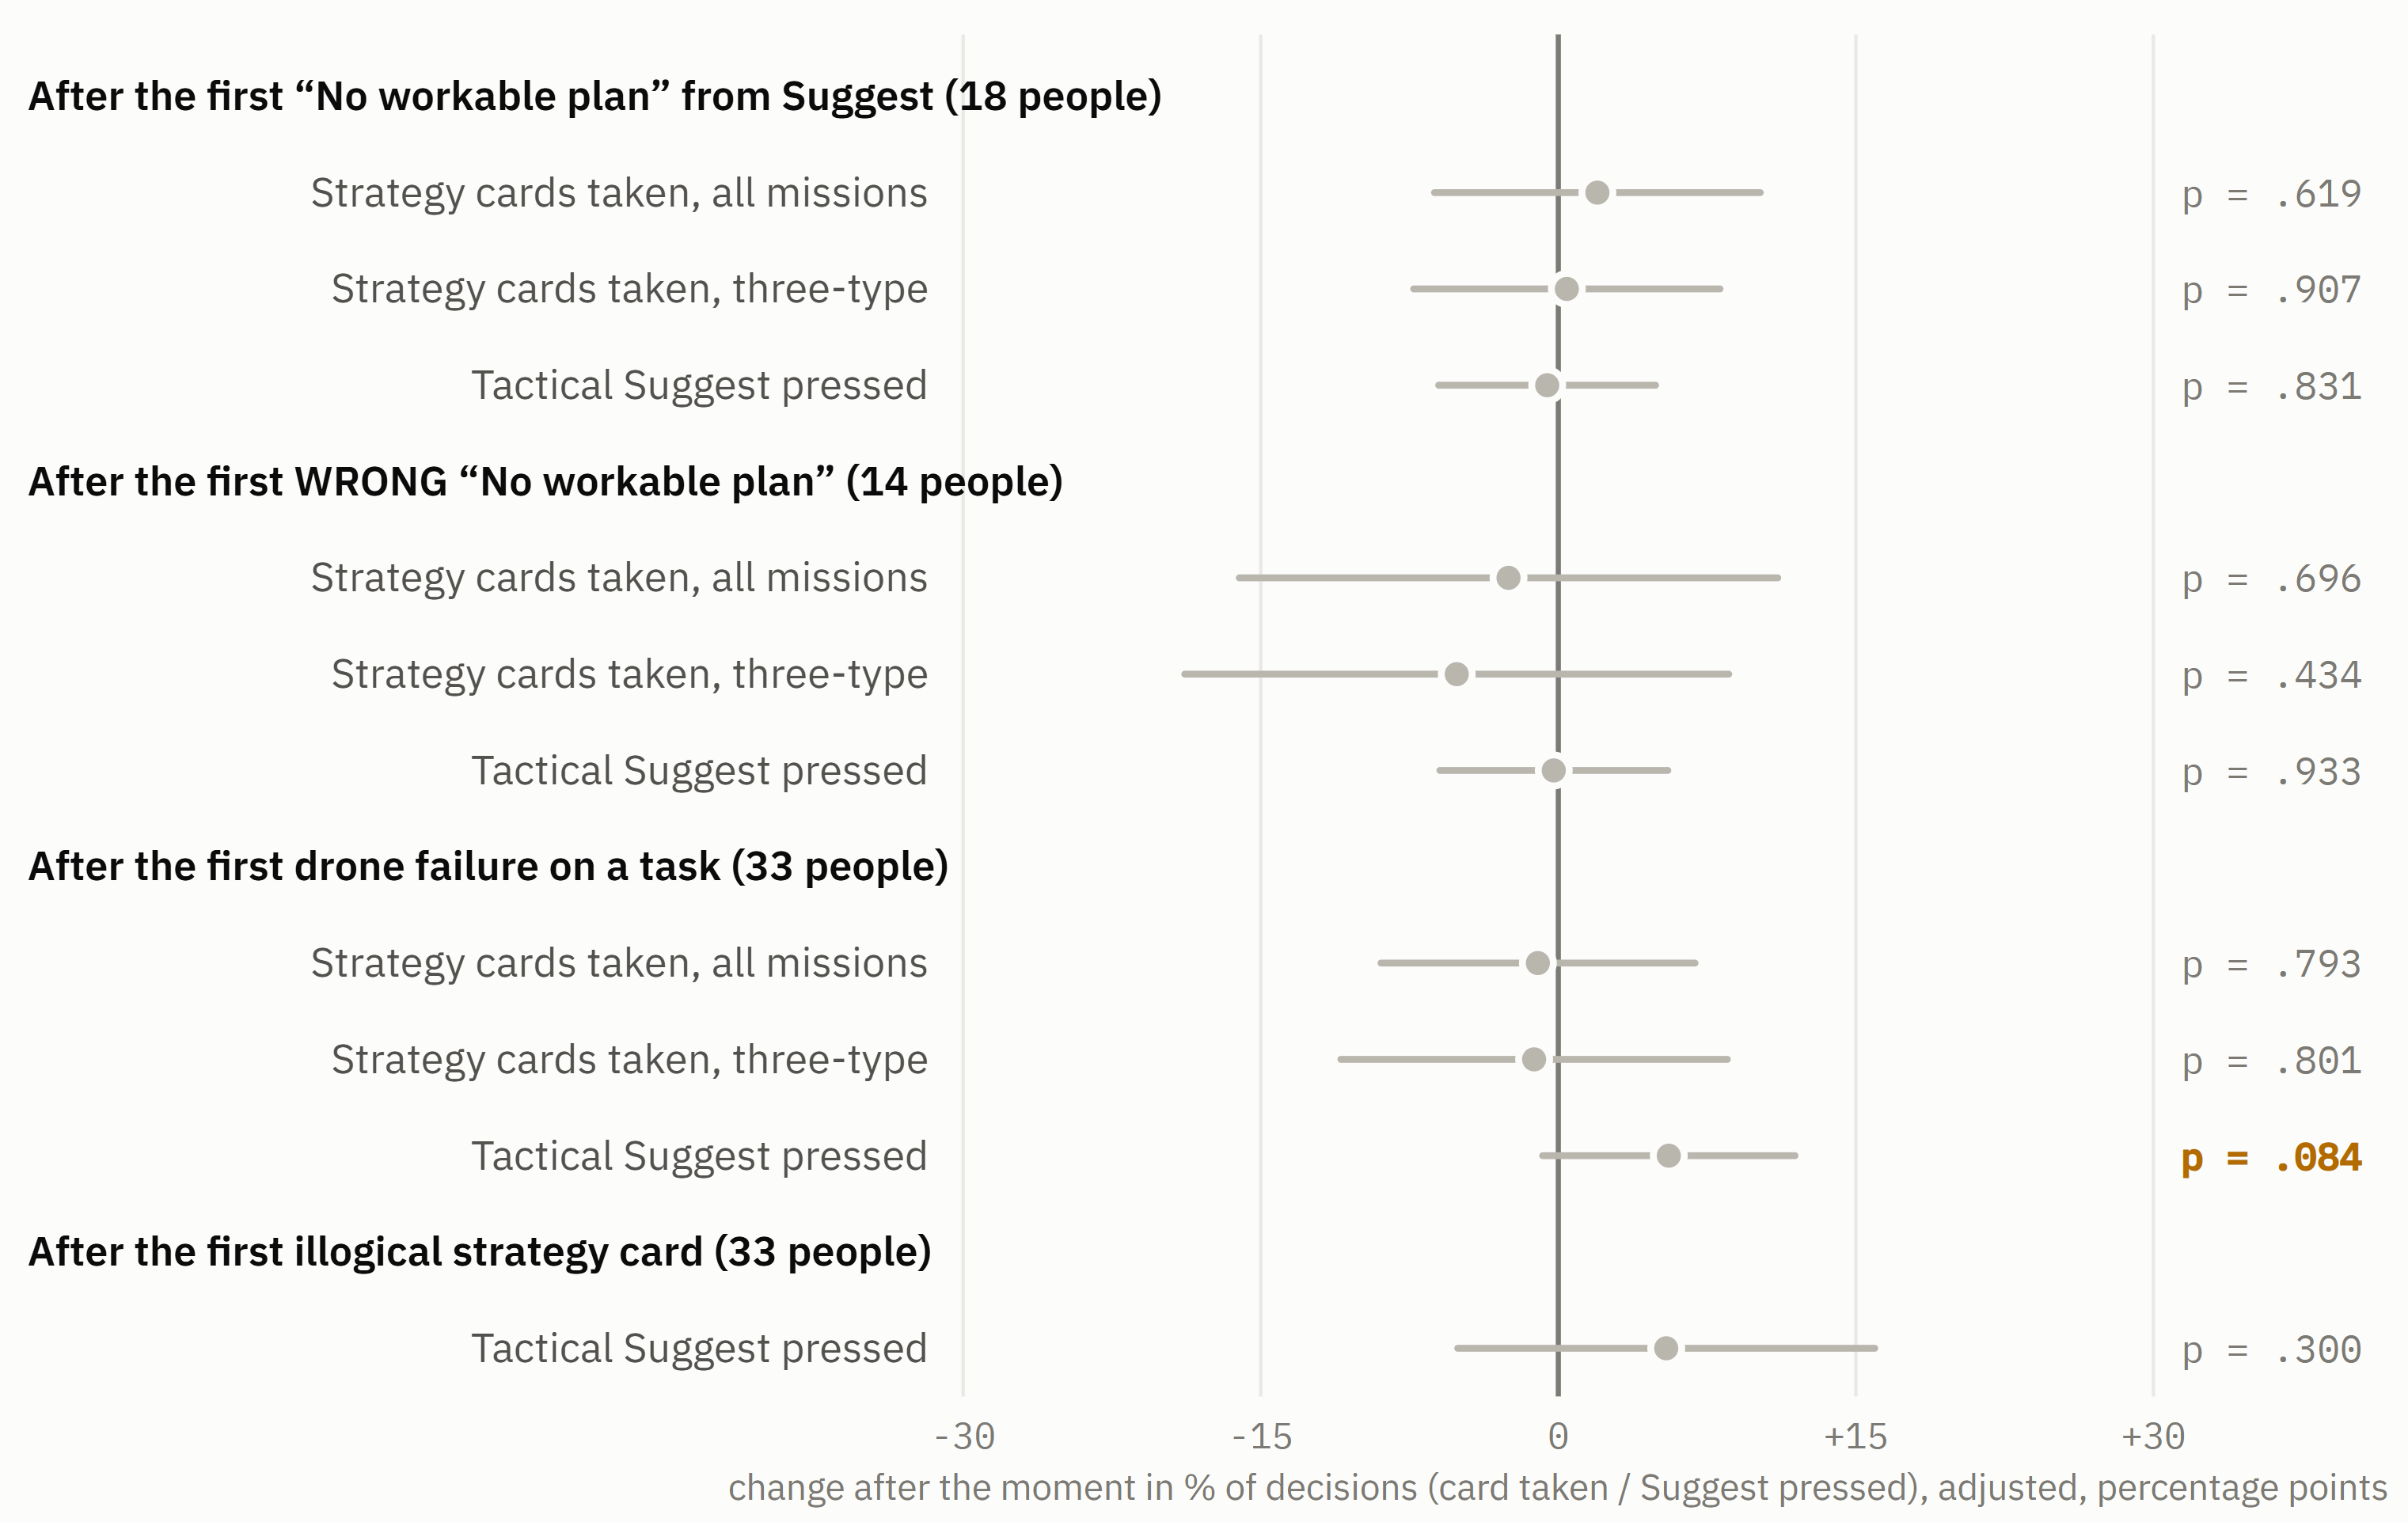
\includegraphics[width=\linewidth,height=0.55\textheight,keepaspectratio]{figs/results/f-flaw-odd__refusal__main.png}
\caption{\textbf{A different event: after the Tactical Assistant's first 'No workable plan', nothing changes on either tier}}
\label{fig:res:flaw-odd:refusal}
\end{figure}

\paragraph*{Key numbers.}

\begin{itemize}[leftmargin=1.2em,itemsep=1pt]

\item First refusal (18): strategy cards, all missions, adjusted +2.0 points [$-$6, +10], p = .62; three-type +0.4, p = .91; tactical Suggest $-$0.6 [$-$6, +5], p = .83

\item First WRONG refusal (14): strategy cards $-$2.5 [$-$16, +11], p = .70; three-type $-$5.1, p = .43; tactical $-$0.2, p = .93

\item First drone failure (33): strategy cards $-$1.0, p = .79; tactical +5.6, p = .08

\item After the first illogical card, tactical Suggest +5.4 points, p = .30 (no spill-down either)

\end{itemize}

\paragraph*{Method.} {\small Same rebuilt method as Section~\ref{sec:res:flaw-odd}. Each person's strategic decisions (or tactical plans) are numbered within the sample, after versus before the moment of their first refusal, with practice held fixed and people clustered. Adjusted = observed minus the expected value. The placebo moves each anchor to a random point drawn from the real anchor positions. All p-values are for the adjusted change.}

\paragraph*{What participants said.} \regtext{Five people reacted aloud to Suggest's 'No workable plan', and every one took it at face value and moved on to abandoning ('Oh well. We'll have to abandon it then') or doing it by hand. Nobody said a refusal made them doubt either assistant. That fits the null. The only counter-voice is P05's note that they would want to check a refusal themself, and P27 asked for the abort button to be highlighted when no plan exists.}

\clearpage

\subsubsection{Why the pre-registered test (H8) was dropped}\label{sec:res:flaw-odd:h8}

\noindent \regtext{H8 asked whether uptake falls after an operator 'realises' the card can be illogical. Its marker for that realisation was the first time a person went manual on an illogical-card mission and left out the unneeded type. The trouble is that, by that definition, every illogical-card decision \emph{before} the marker was not such a manual choice. So the 'before' window was mostly forced to be card takes, near 100\%. Any later manual choice then shows up as a drop, even if the person never changed at all. A simulation confirmed it. In simulated people who keep the same habits all study, the same marker produced a large 'drop' (average odds ratio 0.37, against the real 0.12). Measured against that, the real drop was ordinary (calibrated p = .30, about $-$10 points after correction). Defining the marker as the first manual choice on a \emph{clean} card produced the same kind of drop. H8 was replaced by tests whose anchor is not defined by the outcome (the first illogical card shown; the moment someone said it), each checked against a placebo. Those are the tests in this finding.}

\paragraph*{Key numbers.}

\begin{itemize}[leftmargin=1.2em,itemsep=1pt]

\item Pre-registered estimate OR 0.12; the same test on no-change simulations averages OR 0.37; calibrated p = .30 (risk difference)

\item Placebo marker on clean cards: OR 0.22, p = .03, the same kind of 'drop'

\end{itemize}

\paragraph*{Method.} {\small From docs/analysis/round1/h8\_illogical\_card.md. The null calibration redrew each person's choices 1,000 times from their own constant rate, reapplied the marker and refitted the same model.}

\paragraph*{What participants said.} \regtext{The move the H8 marker counts --- going manual and leaving out the unneeded type --- is described by several (P19, P13, P16, P17, P29). But noticing and going manual are not the same event. Some saw the excess and still took the card (P04, P28 'I still use its suggestion'). Others went manual only to trim an extra of a needed type (P10, P01). So a first manual 'fix' is a poor stand-in for the moment someone realised.}

\clearpage

\subsection{The Tactical Assistant is trusted more, and most people say so too}\label{sec:res:tier-trust}

\regtext{\textbf{Summary.} On the post-session questionnaire, operators trusted the Tactical Assistant more than the Strategic Assistant: 5.44 against 4.61 on a 1--7 scale, 26 of 33 people higher for tactical (p = .001). Most of the gap opens in the second session and in Strategic Heavy games, and people who said in the debrief that they preferred the tactical one also scored it higher. Tactical plans get only a few seconds of checking whatever their size, which fits ``checking is costly, so it is skipped'', but that mechanism test is fragile. Stated trust and actual use line up when people are ranked against each other, but not in size and not over time.} \par\noindent{\small\textit{Strength of evidence (register rating): moderate. Your verdict: keep.}}

\subsubsection{Trusted more: the basic result}\label{sec:res:tier-trust:gap}

\noindent \passtag{for the paper}

\noindent \regtext{After every session operators rated each assistant on the same six statements (``is reliable'', ``I trust its recommendations'', \ldots{}) from 1 to 7. Averaged over their two sessions, \textbf{26 of 33} rated the Tactical Assistant higher, 6 the Strategic Assistant, and 1 the same. The average gap is \textbf{+0.83 points} on the 7-point scale. That is a medium-sized effect (dz = .62), and every one of the six items points the same way.} (Figure~\ref{fig:res:tier-trust:gap})

\begin{figure}[H]
\centering
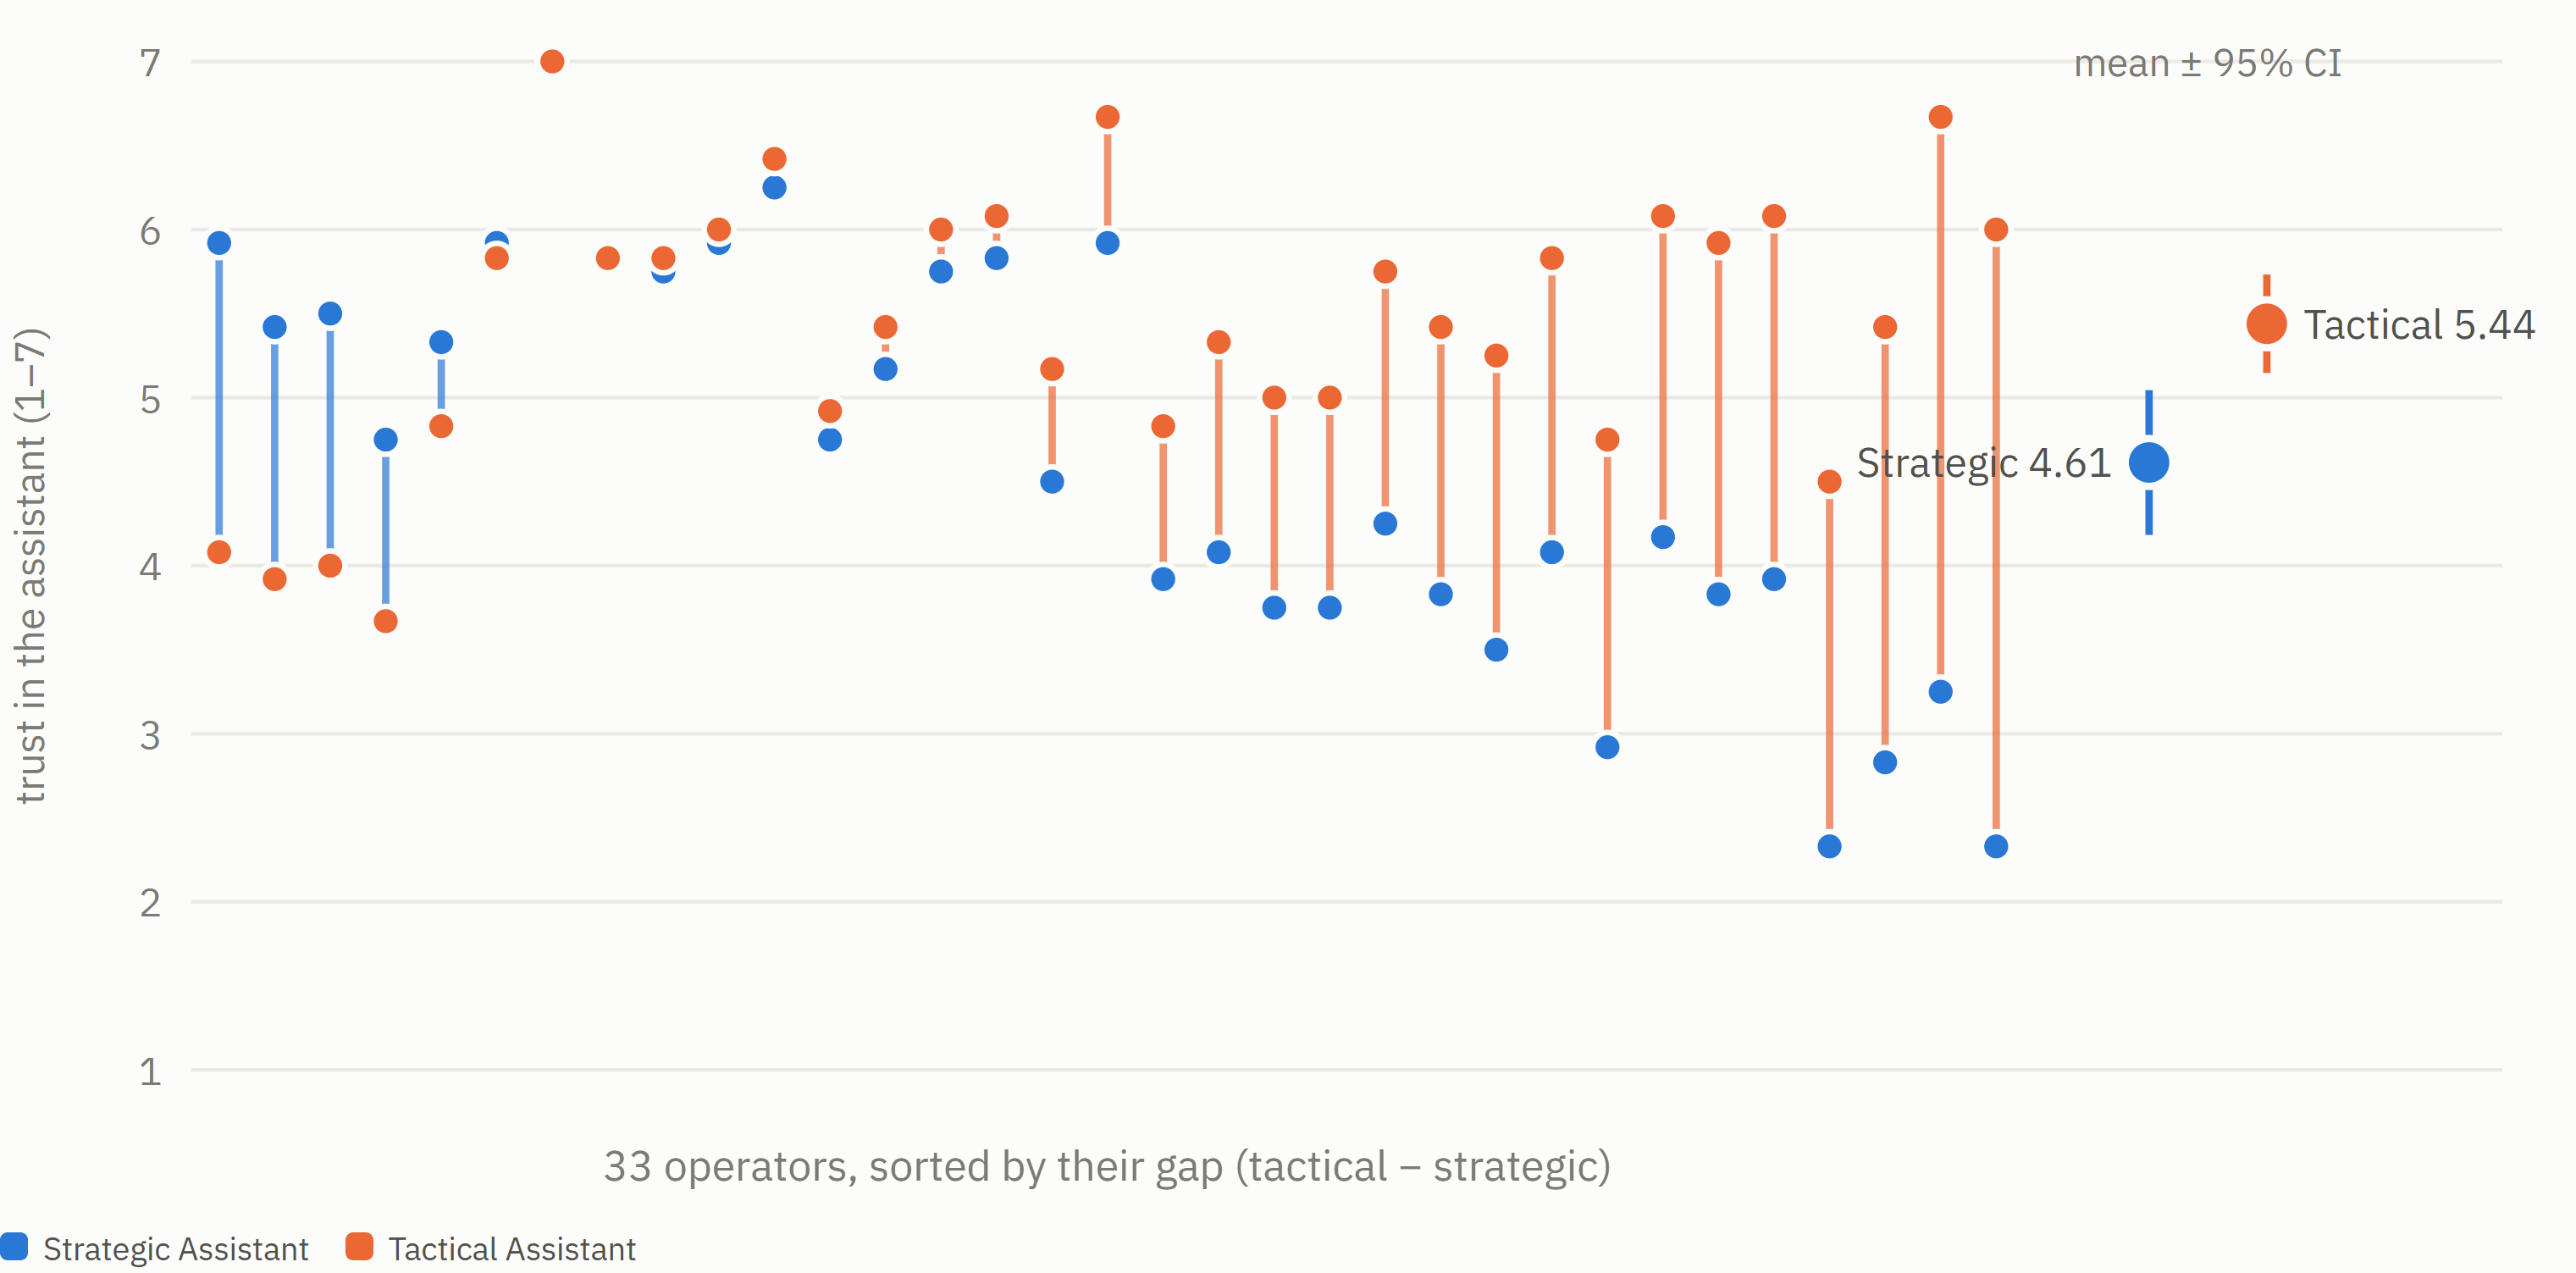
\includegraphics[width=\linewidth,height=0.55\textheight,keepaspectratio]{figs/results/f-tier-trust__gap__main.png}
\caption{\textbf{Trusted more: the basic result}}
\label{fig:res:tier-trust:gap}
\end{figure}

\paragraph*{Key numbers.}

\begin{itemize}[leftmargin=1.2em,itemsep=1pt]

\item Strategic 4.61 [4.18, 5.04], Tactical 5.44 [5.15, 5.73] (1--7, person means)

\item Gap +0.83 [+0.35, +1.30]; paired t p = .0012; Wilcoxon p = .0010; dz = .62; n = 33

\item 26 higher for tactical, 6 for strategic, 1 tied

\item Item gaps: follow its recommendations +1.11, I trust it +1.01, reliable +0.94, performs well +0.74, useful +0.67 (all p < .01); confident in it +0.48 (p = .13)

\end{itemize}

\paragraph*{Method.} {\small One value per person per assistant: the mean of the six items, averaged over that person's two sessions (33 people, P09 excluded). The test is a paired t-test on the difference tactical minus strategic, with a Wilcoxon signed-rank test as the distribution-free check. dz is the mean difference divided by the SD of the differences: .62 means the average person's gap is about six-tenths of the person-to-person spread in gaps. The 95\% CI says the true average gap is very probably between +0.35 and +1.30 points. Items are tested the same way, one at a time.}

\paragraph*{What participants said.} \regtext{In the round-2 preference coding, 17 of 33 favour the Tactical Assistant, 7 the Strategic, 3 both, 4 'it depends' and 2 no view. The usual reason is that the strategic cards visibly waste drones while the tactical plans 'seemed to be doing what I was doing'. Dissent comes from P10, P06 and P07 (trusted strategic more), P31 ('the tactical layer required a little bit more human intervention'), P12 (strategic is the 'more trivial calculation') and P21/P31, who saw tactical flaws (no backup drone, illogical task order).}

\paragraph*{Quotes selected for this section.}

\begin{quotelist}

\item ``But I think in the [tactical level], it works very well.''\,---\,P33 (debrief 0:28:24)

\item ``You can't blame the tactical for drone failures but you can blame the strategic for not having redundancy''\,---\,P03 (written interview)

\item ``So the tactical one seemed to be doing what I was doing. So quite reliably. And obviously the strategic one wasn't.''\,---\,P32 (debrief 0:23:52)

\end{quotelist}

\clearpage

\subsubsection{Where the gap comes from: the second session and the Strategic Heavy scenario}\label{sec:res:tier-trust:where}

\noindent \passtag{for the paper}

\noindent \regtext{The gap is larger in Strategic Heavy sessions (+1.13) than in Tactical Heavy ones (+0.52, CI just reaches zero). It is also small after the first session (+0.37, CI crosses zero) and large after the second (+1.28). Both matter when taken together: holding session order fixed, Strategic Heavy adds about +0.6 to the gap and being the second session about +0.9. Tactical trust hardly moves (5.36 $\rightarrow$ 5.51 across sessions, and only +0.15 between scenarios); it is \textbf{strategic} trust that falls, and it is lowest in Strategic Heavy sessions. So ``trusted more, especially in Strategic Heavy'' largely means ``the strategic one loses trust, especially in the scenario where its cards are used most''. Four people said their trust \emph{grew} with experience (C16). The chart opens on the six questionnaire items (every one favours tactical); \textbf{Scenario played} shows the two scenarios; \textbf{Also: first / second session} shows session order.} (Figure~\ref{fig:res:tier-trust:where})

\begin{figure}[H]
\centering
\begin{subfigure}[t]{0.495\linewidth}
\centering
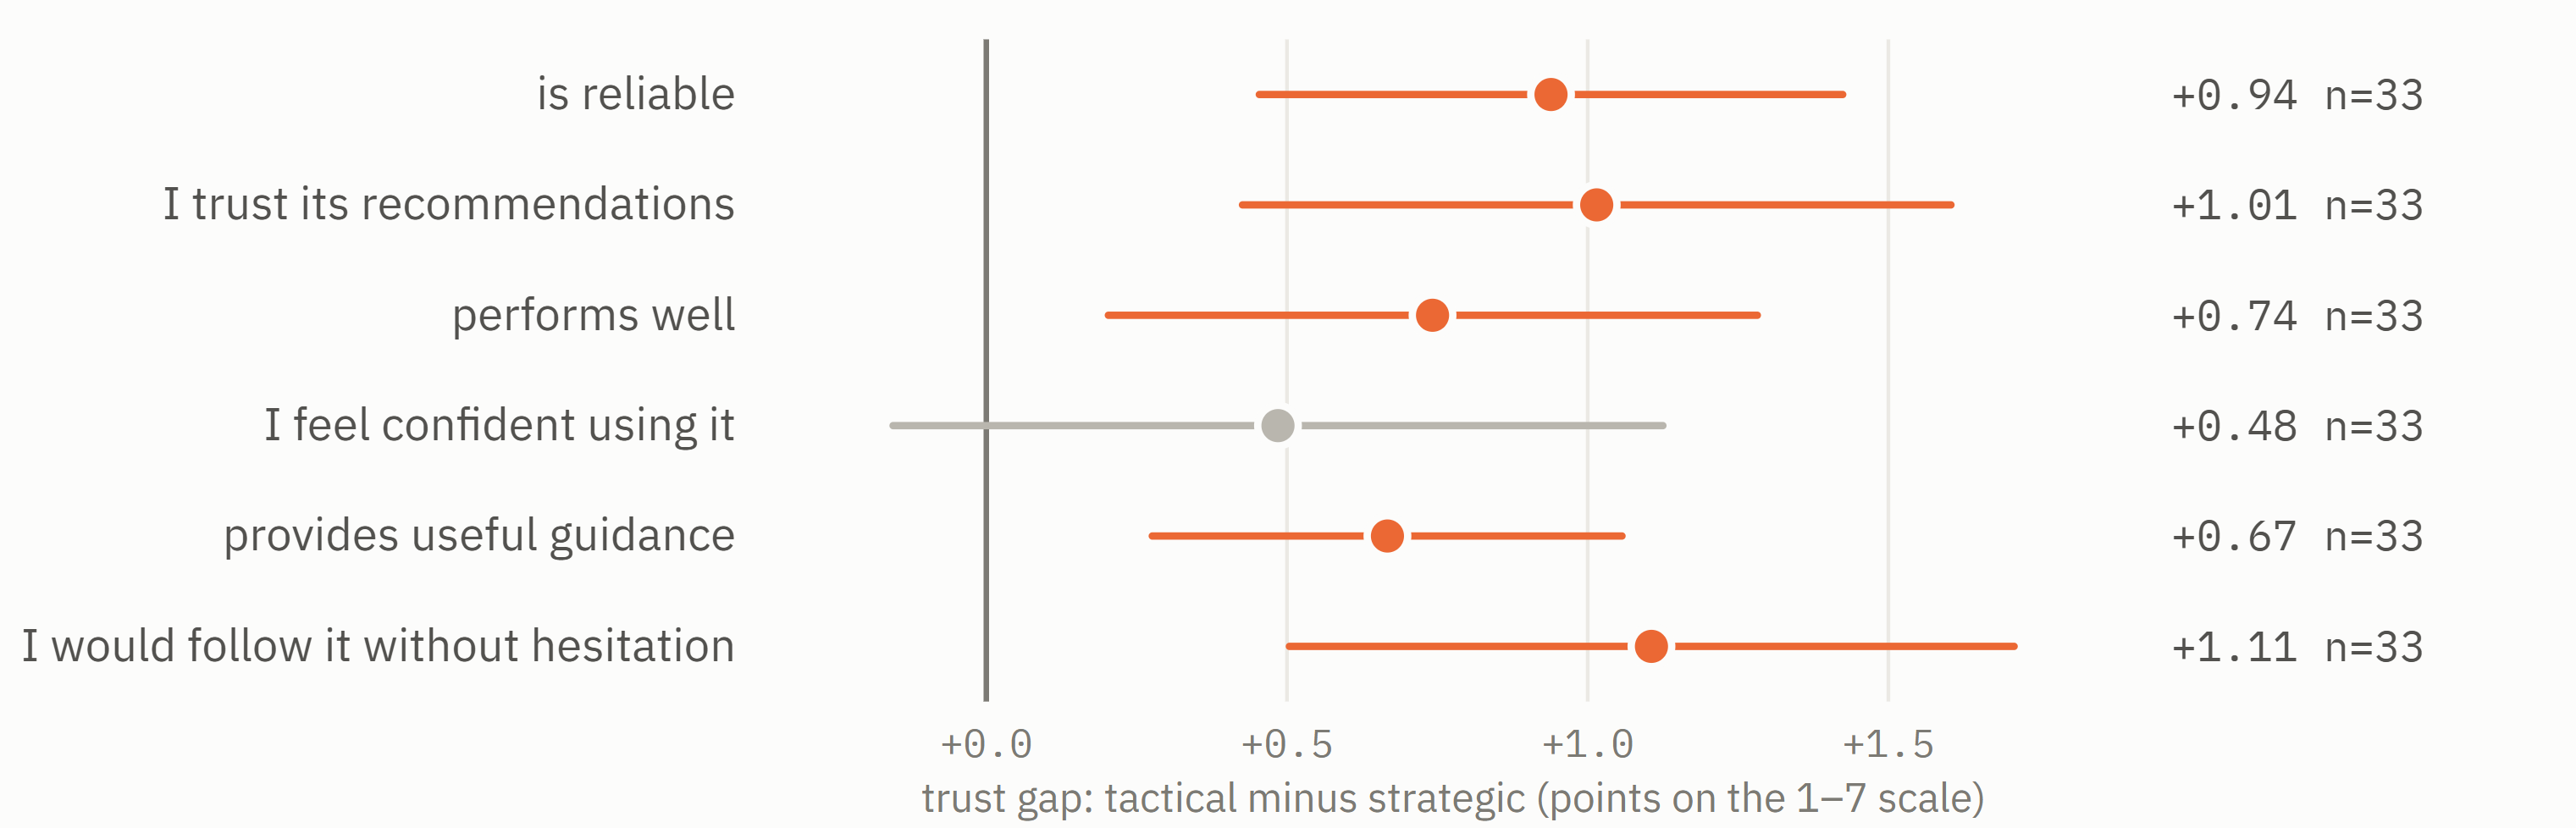
\includegraphics[width=\linewidth,height=0.23\textheight,keepaspectratio]{figs/results/f-tier-trust__where__items.png}
\caption{By questionnaire item.}
\label{fig:res:tier-trust:where:items}
\end{subfigure}
\hfill
\begin{subfigure}[t]{0.495\linewidth}
\centering
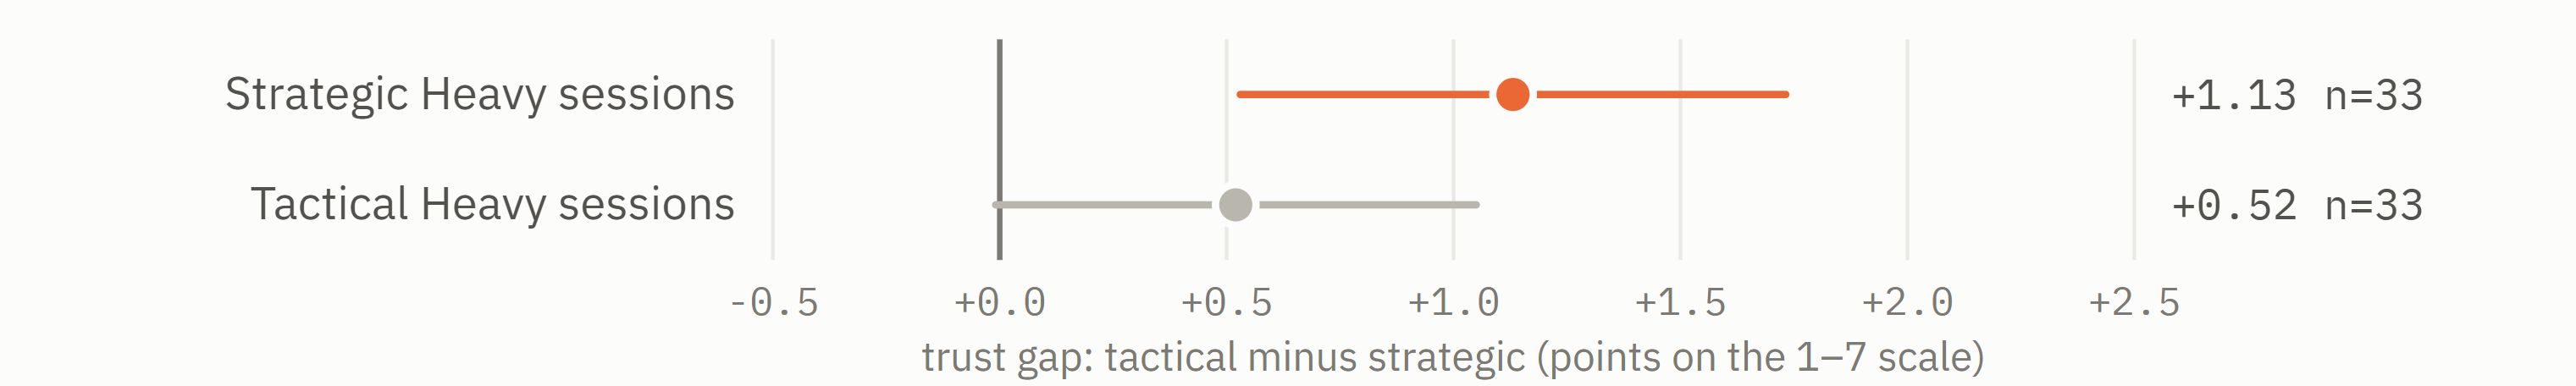
\includegraphics[width=\linewidth,height=0.23\textheight,keepaspectratio]{figs/results/f-tier-trust__where__scenario.png}
\caption{By scenario played.}
\label{fig:res:tier-trust:where:scenario}
\end{subfigure}
\par\smallskip
\begin{subfigure}[t]{0.495\linewidth}
\centering
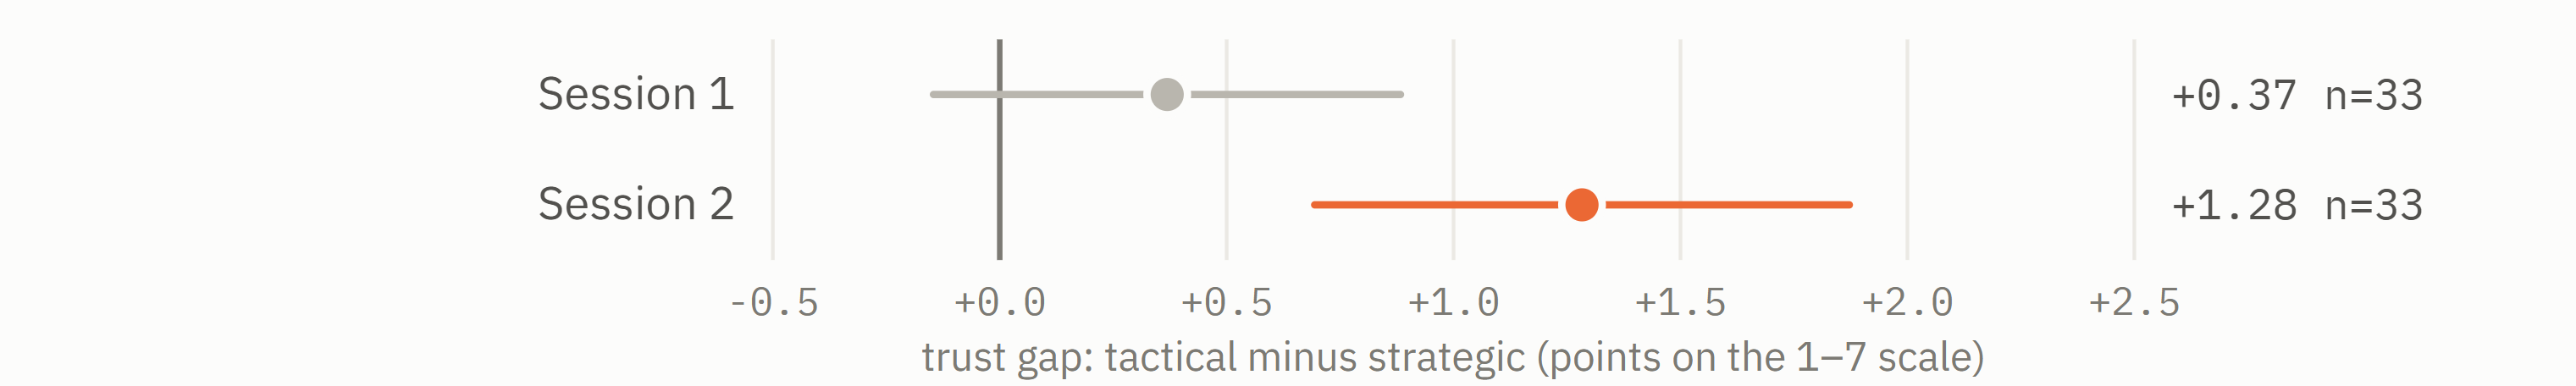
\includegraphics[width=\linewidth,height=0.23\textheight,keepaspectratio]{figs/results/f-tier-trust__where__session.png}
\caption{By session order as well.}
\label{fig:res:tier-trust:where:session}
\end{subfigure}
\hfill
\caption{\textbf{Where the gap comes from: the second session and the Strategic Heavy scenario}}
\label{fig:res:tier-trust:where}
\end{figure}

\paragraph*{Key numbers.}

\begin{itemize}[leftmargin=1.2em,itemsep=1pt]

\item Session 1 gap +0.37 [$-$0.15, +0.88]; session 2 +1.28 [+0.69, +1.87] (n = 33 each)

\item Strategic Heavy sessions +1.13 [+0.53, +1.73]; Tactical Heavy sessions +0.52 [$-$0.01, +1.05] (n = 33 each)

\item Same people, Strategic Heavy minus Tactical Heavy: +0.61 [$-$0.01, +1.23], paired t p = .054, Wilcoxon p = .038; strategic trust $-$0.46 (p = .087), tactical +0.15 (p = .25)

\item Both in one model: Strategic Heavy +0.64 [+0.11, +1.17], p = .019; second session +0.93 [+0.40, +1.47], p < .001

\item Strategic trust 5.00 $\rightarrow$ 4.23 from session 1 to 2; tactical 5.36 $\rightarrow$ 5.51

\end{itemize}

\paragraph*{Method.} {\small The tactical-minus-strategic difference for each session (66 sessions). By session: averaged over the 33 first and the 33 second sessions. By scenario: both games of each scenario pooled (33 sessions each). Every person played one session of each scenario, so the scenario comparison is also done within person (paired t and Wilcoxon on each person's two gaps). Session order and scenario are partly tangled (about half played Strategic Heavy first), so a model with both (GEE, gap \textasciitilde{} Strategic Heavy + second session, clustered by person) separates them. Means have t-based 95\% CIs.}

\paragraph*{What participants said.} \regtext{Those who name a session say it was the strategic tier that slipped in the second session: P19 ('you dropped the ball a little'), P33, P15 and P17. Tactical trust was steady or up (P19, P26). Against the pattern, P06 says strategic trust went up over time and P20 saw strategic issues only in the first run. Nobody tied the change to the Strategic Heavy scenario as such.}

\clearpage

\subsubsection{Why the tactical plan is kept: checking it is brief and does not grow with the plan}\label{sec:res:tier-trust:checking}

\noindent \passtag{for the paper}

\noindent \regtext{Bigger missions mean bigger tactical plans. As plans grow, operators press Suggest more often (63\% of plans with 3 or fewer drones $\rightarrow$ 93\% with 10 or more) and keep the plan unmodified more often (63\% $\rightarrow$ 86\%). Once Deploy unlocks, they spend a median of about \textbf{2--4 seconds} on the plan whatever its size. Per drone, checking therefore falls steeply as plans grow (0.7 s $\rightarrow$ 0.2 s). A strategy card gets about 9 s. Almost every consulted plan is deployed as it comes: 468 of 486. The more there is to check, the less of it is checked proportionally, and the plan is taken. Operators describe exactly this. Nine say they check when it is cheap and skip it under pressure (C17). Three say the plan was too complex or too fast to check (C14). Five say they checked nearly everything, and they do decide more slowly (C18). Only 3 of 33 ever mention noticing a tactical flaw (C13). \par \par \textbf{But} the pre-registered mechanism test (H2) is fragile. All three predicted parts point the right way (p = .019 uncorrected), but it does not survive correction for the round's several tests (.065). Among consulted plans, larger ones are actually modified a little \emph{more}. Keeping goes up with size mainly because people consult more on big plans, not because they check consulted plans more lightly. The logs also cannot tell ``too costly to check'' apart from ``nothing ever looked wrong''. The tactical plan's flaws are hard to see, while the cards' over-allocation is visible. That half of the explanation belongs to \emph{tier-flaw-visibility} in Section~\ref{sec:res:flaw-odd} and is not repeated here.} (Figure~\ref{fig:res:tier-trust:checking})

\begin{figure}[H]
\centering
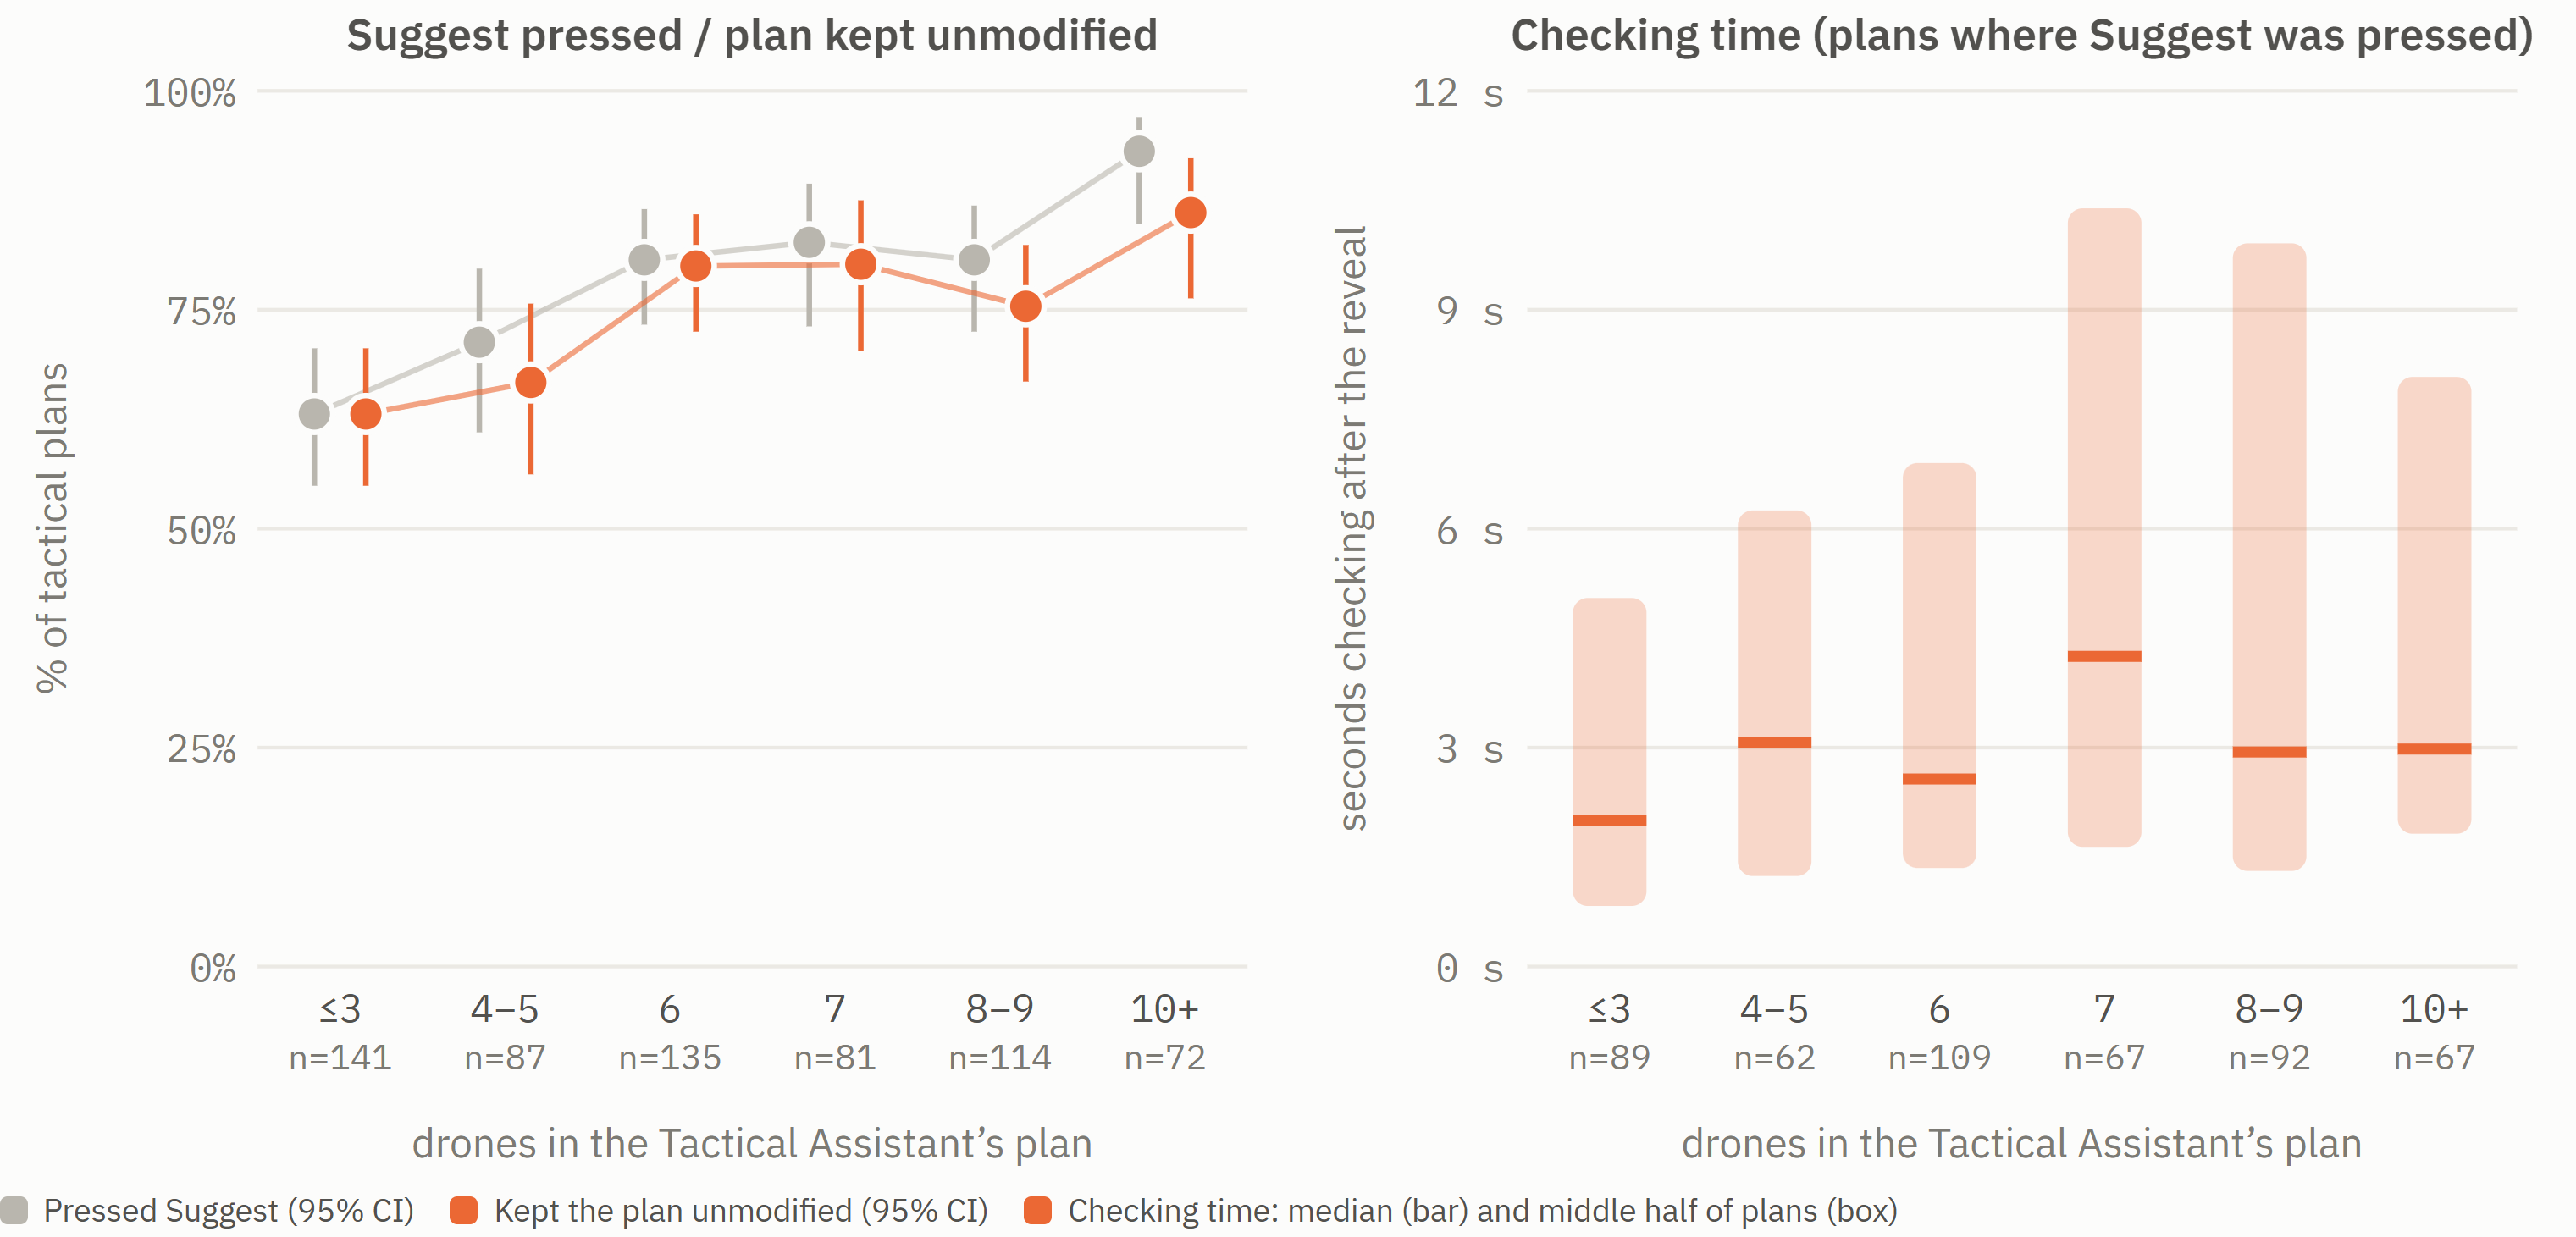
\includegraphics[width=\linewidth,height=0.55\textheight,keepaspectratio]{figs/results/f-tier-trust__checking__main.png}
\caption{\textbf{Why the tactical plan is kept: checking it is brief and does not grow with the plan}}
\label{fig:res:tier-trust:checking}
\end{figure}

\paragraph*{Key numbers.}

\begin{itemize}[leftmargin=1.2em,itemsep=1pt]

\item Kept unmodified rises with plan size: OR 1.76 per SD [1.25, 2.47], p = .001 (all 630 plans)

\item Consulted rises: OR 2.52 [1.87, 3.38]; kept once consulted FALLS: OR 0.68 [0.50, 0.94], p = .017

\item By bin ($\leq$3, 4--5, 6, 7, 8--9, 10+ drones; n = 141, 87, 135, 81, 114, 72 plans): Suggest pressed 63\%, 71\%, 81\%, 83\%, 81\%, 93\%; kept unmodified 63\%, 67\%, 80\%, 80\%, 75\%, 86\%

\item 10+ drones vs $\leq$3: Suggest pressed 93\% vs 63\%, OR 10.8 [3.2, 36.0]; kept 86\% vs 63\%, OR 5.2 [2.1, 12.7], both p < .001

\item Median checking time by bin: 2.0, 3.1, 2.6, 4.2, 2.9, 3.0 s; per SD +0.60 s [$-$0.15, +1.35], p = .12; per drone 0.68 s at $\leq$3 drones $\rightarrow$ 0.23 s at 10+

\item 468 of 486 consulted plans deployed unmodified (96\%)

\item Person-median check: tactical 2.85 s vs strategy card 8.80 s (n = 33, Wilcoxon p < .0001)

\item H2 primary p = .019 uncorrected, .065 after Holm correction across round 1

\end{itemize}

\paragraph*{Method.} {\small 630 confirmed tactical plans from 33 people (h2\_verification\_cost.load). They are grouped by the number of drones in the Tactical Assistant's plan into six bins with no gaps: $\leq$3, 4--5, 6, 7, 8--9 and 10+ drones. The bins were chosen so every bin has enough plans for a stable rate: at least 72 plans and at least 62 with a checking time in each (the smallest bins are 4--5 drones, 87 plans, and 10+, 72 plans). Every plan is used; none is dropped. ``Consulted'' means Suggest was pressed at least once. ``Kept unmodified'' means consulted and deployed with no change. ``Checking time'' runs from the last Suggest press to Deploy, minus the forced reveal: the planner adds one drone$\rightarrow$task pair per second and Deploy is locked until it finishes, so that wait is not checking. Effects per SD of plan size (drones $\times$ tasks) come from GEE models on all 630 plans, clustered by person, adjusted for scenario and session; they do not depend on the bins. An odds ratio of 1.76 means each step up in plan size multiplies the odds of keeping the plan by 1.76. The two ends (10+ vs $\leq$3 drones) are also compared directly. The card comparison takes each person's median net decision time on strategic decisions: strategic\_choice latency minus the card reveal, over all strategic decisions, manual ones included. The H2 numbers are from docs/analysis/round1/h2\_verification\_cost.md.}

\paragraph*{What participants said.} \regtext{Speaking to this point: 3 of 33 say the tactical plan was too complex or fast to check (C14), 9 that checking depended on time (C17), and 5 that they always checked (C18). The reasons match the finding: the plan is hard to check, so it is taken on trust ('I just took the AI's word for it'). Several say it is not more trust but the time to check (P04). P14 is the clear dissent: they checked tactical plans more, drone by drone, because cards can be read 'in one glance'.}

\paragraph*{Quotes selected for this section.}

\begin{quotelist}

\item ``as soon as it got to any sort of non-linear, difficult, high dimensional problem, I just took the AI's word for it, essentially, probably because I couldn't assess in the time''\,---\,P22 (debrief 0:30:06)

\item ``My reason is there are so many drones, so I don't have enough energy and attention to just the check them.''\,---\,P27 (think-aloud s1 0:56)

\end{quotelist}

\clearpage

\subsubsection{Stated vs revealed preference: they line up in rank, not in size or over time}\label{sec:res:tier-trust:stated-revealed}

\noindent \passtag{numbers only}

\noindent \regtext{Does the person who \emph{says} (rates) the Tactical Assistant higher also \emph{lean} on it more? Ranked against each other, yes, moderately. The person-level trust gap correlates $\rho$ = .47 with the usage gap (share of tactical plans kept unmodified minus share of strategic decisions where a card was taken). 16 people favour tactical on both measures and 3 favour strategic on both. Three things do \textbf{not} line up: \par (1) \textbf{Size.} Stated trust favours tactical strongly (26 of 33), but use barely does. Cards are taken on 64\% of strategic decisions and tactical plans kept on 72\%, a gap of +8 points whose CI includes zero. Nine people rate tactical higher yet use the strategic cards more. \par (2) \textbf{Change.} Within a person, a rise or fall in trust from session 1 to 2 does not go with a matching change in use ($\rho$ = .16 strategic, .13 tactical). \par (3) \textbf{Lead.} Session-1 trust does not predict how card use changes in session 2 ($\rho$ = .07). Trust ratings read like a stable opinion of the assistant, while use follows the moment: mission size, queue, time. The ratings describe the person; they do not forecast their next move.} (Figure~\ref{fig:res:tier-trust:stated-revealed})

\begin{figure}[H]
\centering
\begin{subfigure}[t]{\linewidth}
\centering
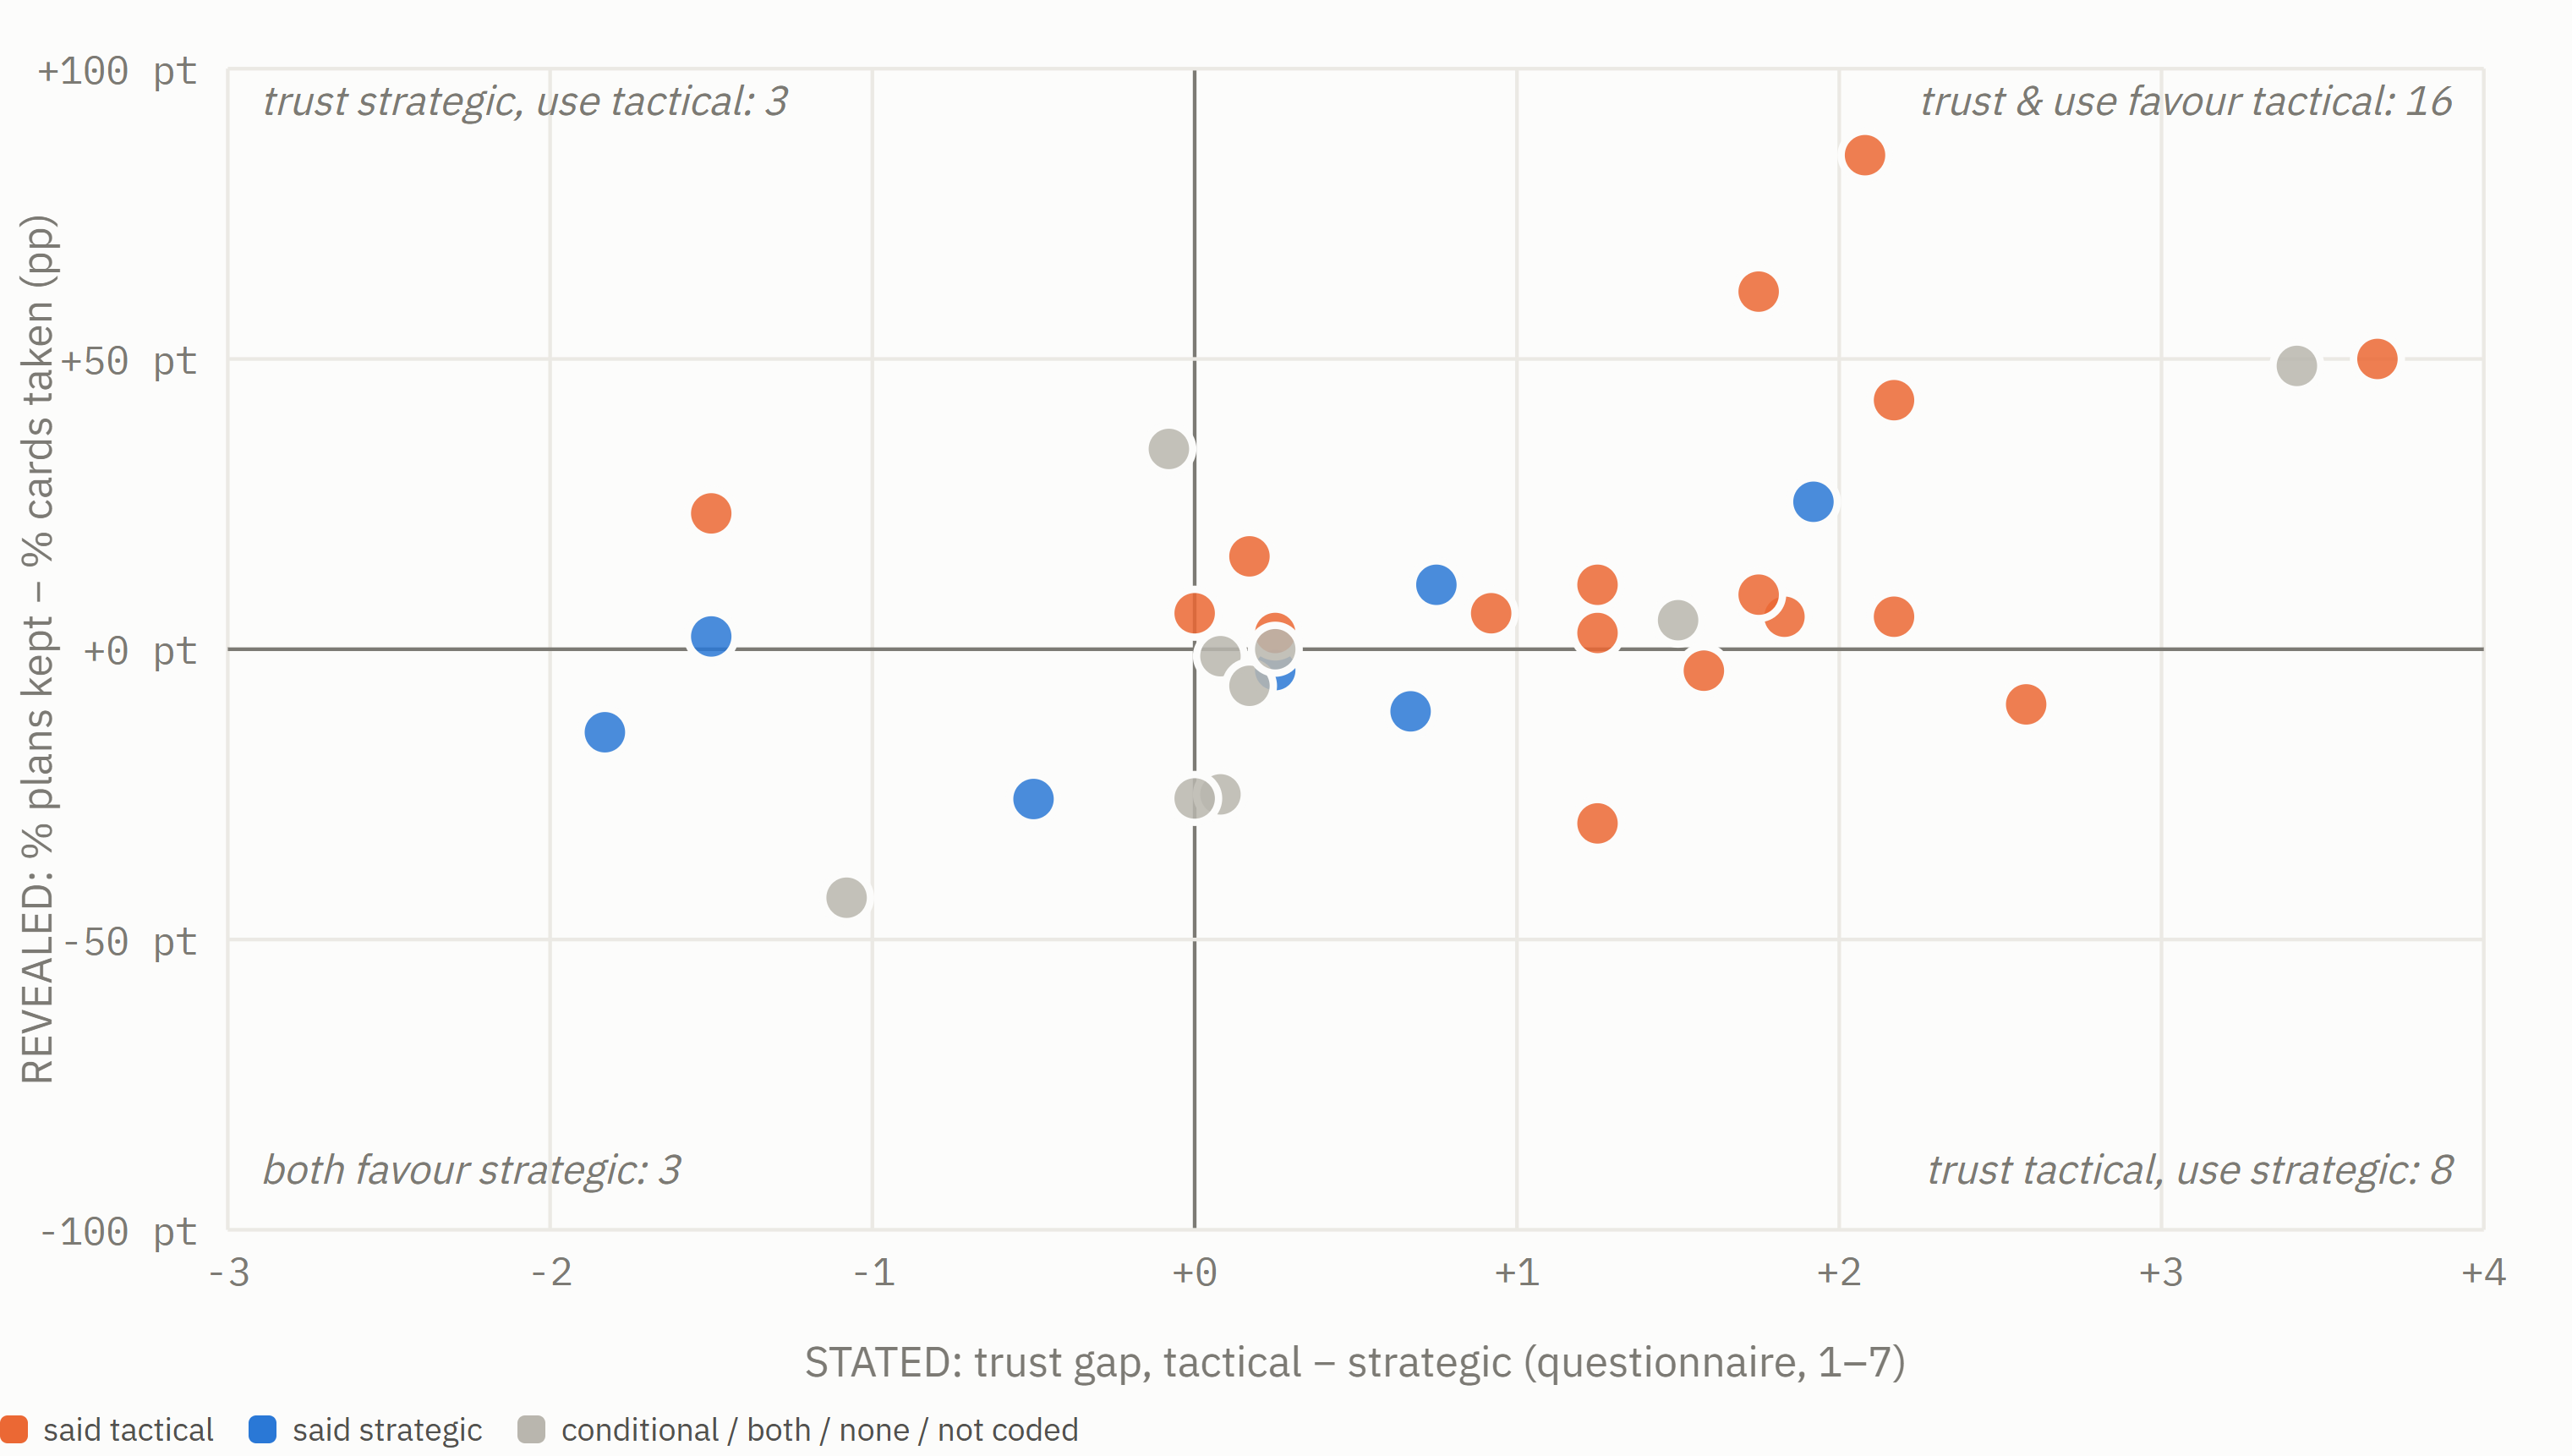
\includegraphics[width=\linewidth,height=0.23\textheight,keepaspectratio]{figs/results/f-tier-trust__stated-revealed__kept.png}
\caption{Use measured as keeping the plan unmodified.}
\label{fig:res:tier-trust:stated-revealed:kept}
\end{subfigure}
\par\smallskip
\begin{subfigure}[t]{\linewidth}
\centering
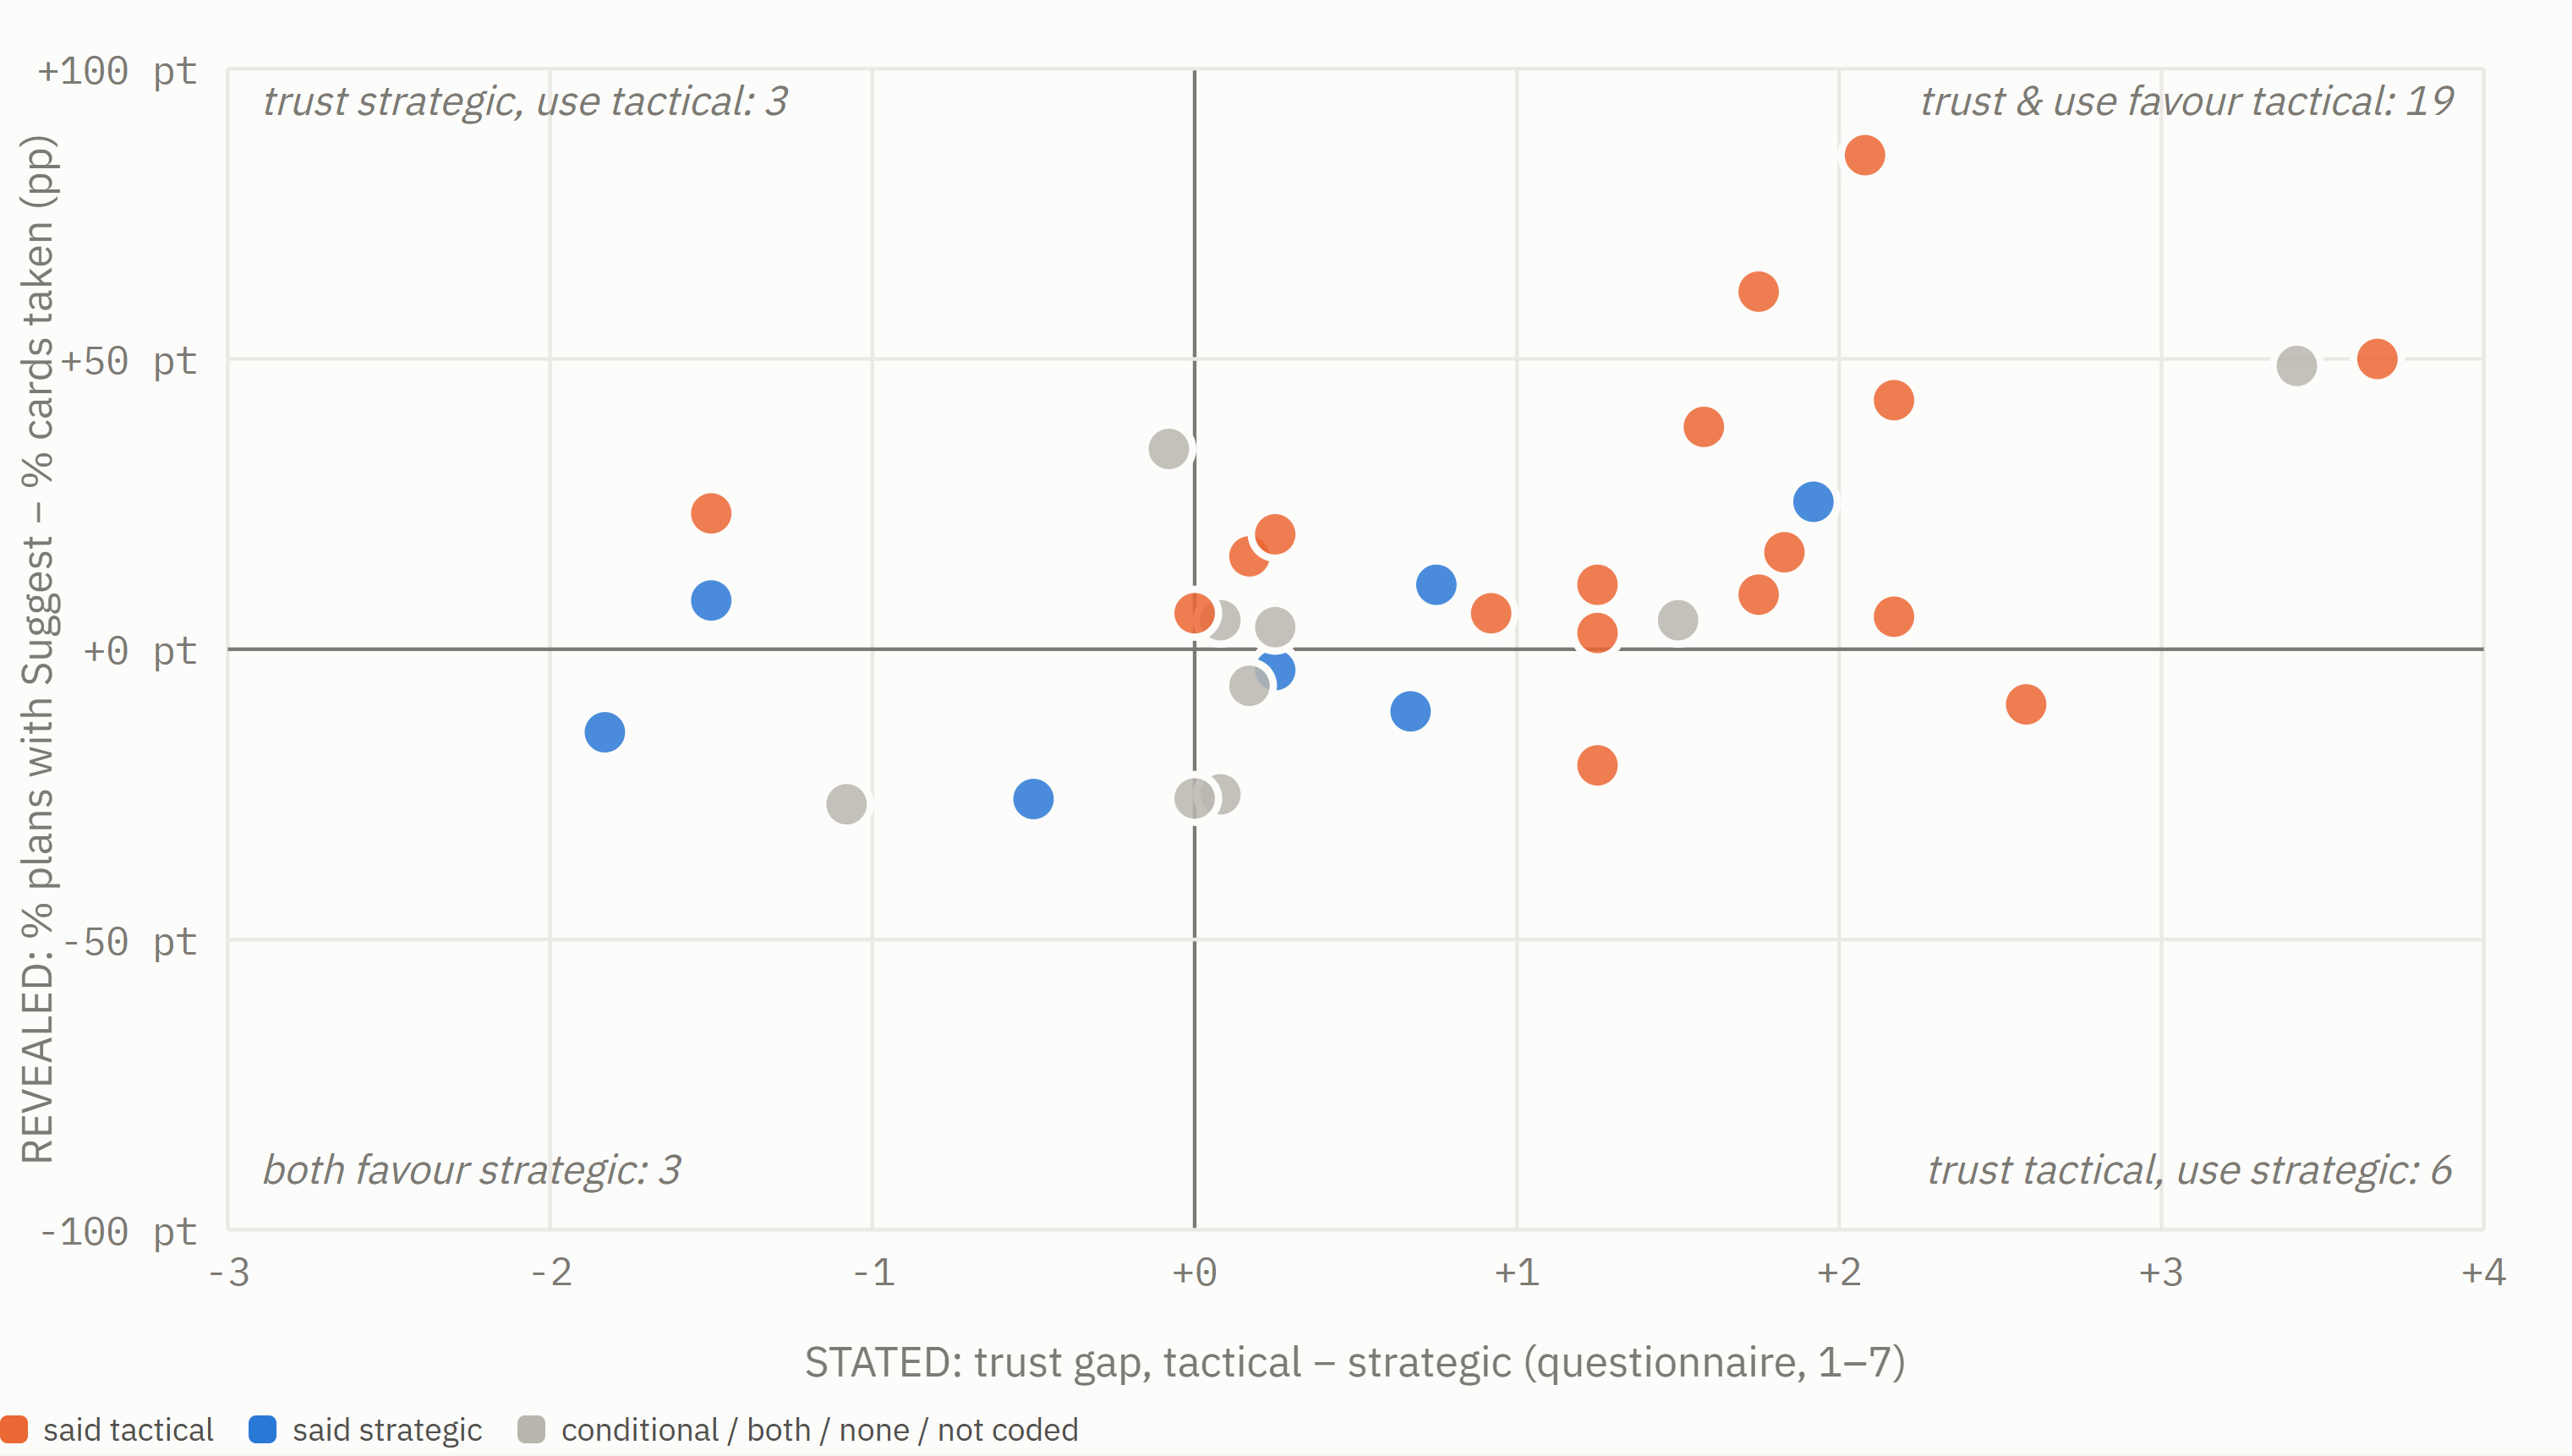
\includegraphics[width=\linewidth,height=0.23\textheight,keepaspectratio]{figs/results/f-tier-trust__stated-revealed__pressed.png}
\caption{Use measured as pressing Suggest at all.}
\label{fig:res:tier-trust:stated-revealed:pressed}
\end{subfigure}
\par\smallskip
\caption{\textbf{Stated vs revealed preference: they line up in rank, not in size or over time}}
\label{fig:res:tier-trust:stated-revealed}
\end{figure}

\paragraph*{Key numbers.}

\begin{itemize}[leftmargin=1.2em,itemsep=1pt]

\item Trust gap vs usage gap (kept $-$ took): $\rho$ = .47 [.10, .73], p = .006, n = 33

\item Quadrants: both favour tactical 16, both strategic 3, trust tactical/use strategic 9, trust strategic/use tactical 3 (2 on a zero line)

\item Group use: took a card 64\%, consulted the plan 76\%, kept it 72\%; usage gap +0.08 [$-$0.02, +0.17]

\item Within person, change in strategic trust vs change in card use: $\rho$ = .16 [$-$.27, .52], p = .38

\item Session-1 strategic trust vs change in card use s1$\rightarrow$s2: $\rho$ = .07 [$-$.27, .40], p = .71; tactical .01

\item Between people, strategic trust vs cards taken $\rho$ = .60 [.30, .78]; tactical trust vs plan kept $\rho$ = .31, p = .08

\end{itemize}

\paragraph*{Method.} {\small One dot per person, both sessions pooled. Stated = mean tactical trust minus mean strategic trust (1--7). Revealed = share of their confirmed tactical plans kept unmodified minus share of their strategic decisions where they took a card (the alternative ``pressed Suggest at all'' gives the same picture, $\rho$ = .49). Spearman $\rho$ uses 4000-draw seeded bootstrap CIs. A caveat on (1): taking a card and keeping a plan are different acts with different costs, so the \emph{level} of the usage gap is not a pure preference; the ranking is the cleaner comparison. ``Change'' correlates the session-2 minus session-1 differences within each person (33 people). ``Lead'' correlates session-1 trust with the later change in use. Session-level links are also shown (66 sessions): strategic trust \textasciitilde{} cards taken $\rho$ = .49, tactical trust \textasciitilde{} plan kept $\rho$ = .27. Note that the trust survey comes \emph{after} the session it follows, so a same-session link can be use shaping trust as easily as the reverse.}

\paragraph*{What participants said.} \regtext{Several people say outright that how much they used an assistant was not the same thing as how much they trusted it. They took cards they rated lower because cards save time ('less reliable\ldots{} but I still use its suggestion', P28). P20 lost trust in the strategic tier yet found it 'a bit more useful', and P11 would 'miss both equally' but use the strategic one more. This matches the gap between trust and use found in the data.}

\clearpage

\subsubsection{All the trust--use correlations in one view}\label{sec:res:tier-trust:trust-lead-strip}

\noindent \passtag{numbers only}

\noindent \regtext{Between people, trust and use move together, most clearly for the strategic tier. Within a person over time, and as a predictor of the next session, the correlations are near zero.} (Figure~\ref{fig:res:tier-trust:trust-lead-strip})

\begin{figure}[H]
\centering
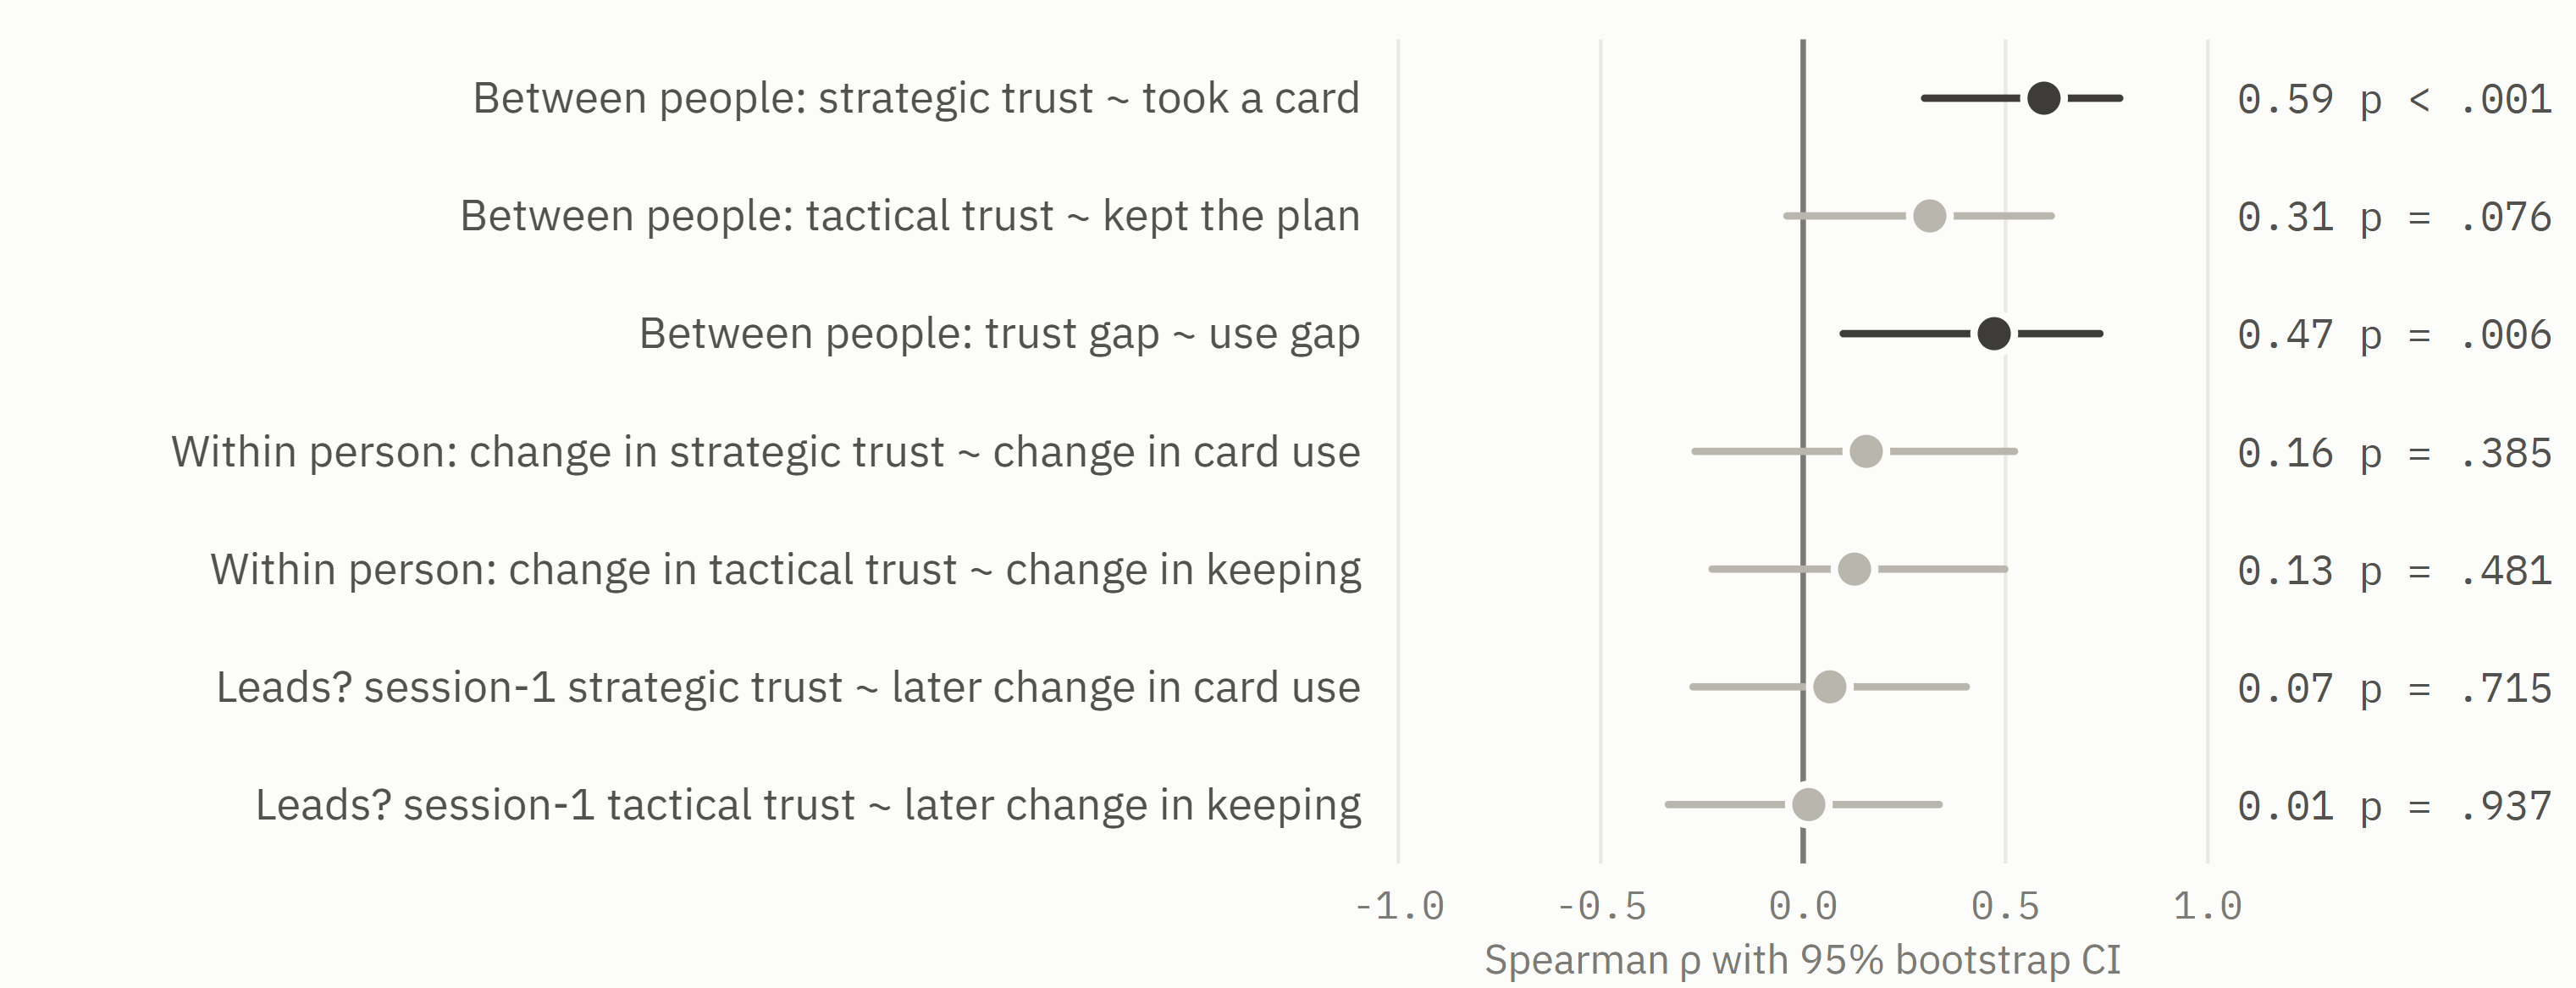
\includegraphics[width=\linewidth,height=0.55\textheight,keepaspectratio]{figs/results/f-tier-trust__trust-lead-strip__main.png}
\caption{\textbf{All the trust--use correlations in one view}}
\label{fig:res:tier-trust:trust-lead-strip}
\end{figure}

\paragraph*{Method.} {\small Each row is a Spearman $\rho$ with a 4000-draw seeded bootstrap 95\% CI, at the person level (n = 33). A dark dot means p < .05. These are the same numbers as the section above, in one picture.}

\paragraph*{What participants said.} \regtext{4 of 33 say their trust grew with experience or success (C16: P06, P10, P26, P32), and a few more describe a checking-then-trusting arc in play (P07, P06, P29). These accounts are all retrospective and smooth, while the data show no within-person link from trust to later use. Nobody describes trust falling and use following it within a session.}

\clearpage

\subsection{Beyond the findings: what operators said they want, believe and feel}\label{sec:res:operator-wants}

\regtext{\textbf{Summary.} Asked about real search and rescue, nobody rejected assistants like these, and 9 of 33 said a human must keep the final decision. What they asked for was mostly information: how the assistants decide (about 12) and failure risk or feedback on how they were doing (11). Some wanted help with a decision neither tier covers, choosing which mission to open next (P27, P32). How they pictured the assistants ranged from ``a dozen lines of code'' to something that learns or predicts, and several credited them with more than they had (learning from the operator, prediction, one shared plan across the tiers). Suggestive: one coder, and much of it unprompted talk during play.} \par\noindent{\small\textit{Strength of evidence (register rating): suggestive. Your verdict: keep.}}

\subsubsection{What they asked for}\label{sec:res:operator-wants:wants}

\noindent \passtag{numbers only}

\noindent \regtext{The common thread is control plus information: keep the human in the decision and give them more to decide with (why the assistant suggested it, how likely drones are to fail, options in between). Only four wanted the assistant to do more. These are design requirements more than findings --- and the ``reasoning'' request links to the tactical blind spot, where an explained refusal could have been checked.} (Figure~\ref{fig:res:operator-wants:wants})

\begin{figure}[H]
\centering
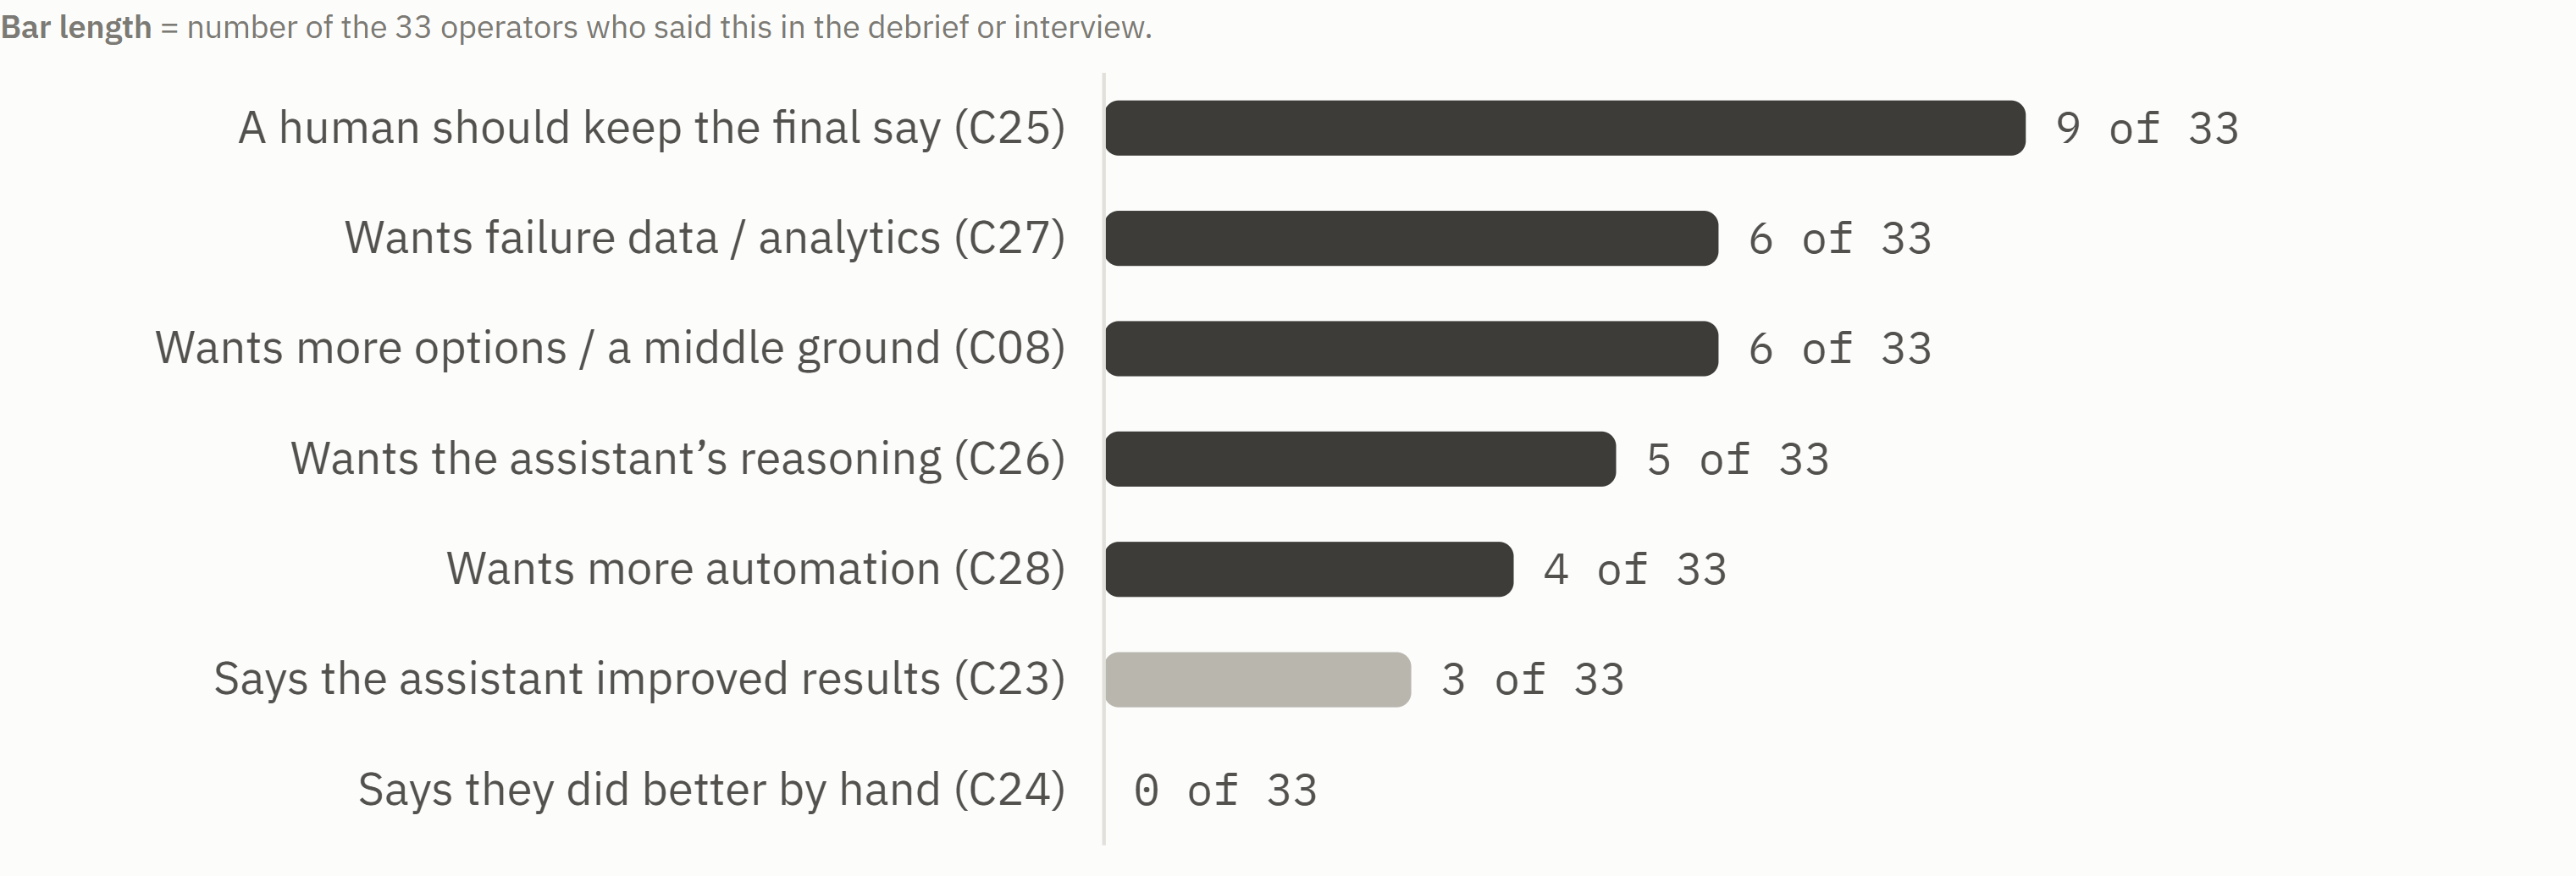
\includegraphics[width=\linewidth,height=0.55\textheight,keepaspectratio]{figs/results/f-operator-wants__wants__main.png}
\caption{\textbf{What they asked for}}
\label{fig:res:operator-wants:wants}
\end{figure}

\paragraph*{Key numbers.}

\begin{itemize}[leftmargin=1.2em,itemsep=1pt]

\item Human final say 9 of 33 (8 unprompted); failure data 6; more options 6; reasoning 5; more automation 4 (all unprompted)

\end{itemize}

\paragraph*{Method.} {\small Debrief transcripts and interview notes coded against the codebook (CODEBOOK.md): C25 human final say, C27 failure data, C08 middle ground / more options, C26 reasoning, C28 more automation. ``Unprompted'' = at least one piece of evidence not given as a bare yes to a leading question.}

\paragraph*{What participants said.} \regtext{Across the coded material, 9 of 33 said a human should keep the final say (8 unprompted), 6 wanted failure probabilities or performance data, 6 wanted options between the two cards, 5 wanted the assistant's reasoning and 4 wanted more automation. Reading everything (including the in-play talk) raises the information asks: about 11 asked or wondered how the assistants decided, and 8 asked for failure or performance numbers. The dissent is small but sharp: P11 does not want to be 'reduced to pressing allocate, suggest, deploy'. The mini sections below take each strand in turn.}

\clearpage

\subsubsection{Real search and rescue: welcome, with a human deciding}\label{sec:res:operator-wants:real-world}

\noindent \passtag{extra: may make it in}

\noindent \regtext{What people said when asked how they would feel about systems like this in real search and rescue. 16 of 33 are quoted here (25 answered the question); nobody rejected it, and the common condition was a human who keeps the final decision.}

\paragraph*{What participants said.} \regtext{Asked the closing 'five years from now' question, at least 14 welcomed the idea, nearly always for speed ('a bad approximation is better than no response at all'), and 9 said a human must keep the final decision (8 unprompted). Conditions came with it: well regulated (P20), only where the job is understood and stakes low (P03, P05), only if better than today's AI (P15). Others raised a deeper worry: who is accountable when an AI fails to save someone (P31, P22), and military use of the research (P31). When pressed on whether a busy human could really check, P24 conceded they could not and still wanted one there.}

\clearpage

\subsubsection{Wanting to know how the assistants decide}\label{sec:res:operator-wants:reasoning}

\noindent \passtag{extra: may make it in}

\noindent \regtext{Requests for the assistants' reasoning, and moments where people could not work out why a card or plan looked the way it did. 12 of 33 said something on this.}

\paragraph*{What participants said.} \regtext{5 of 33 asked outright for explanation, auditability or understandable tools (P02, P12, P16, P25, P36); 6 more asked mid-play why a card looked as it did or said they could not tell (P01, P05, P06, P13, P25 in play, P32). P01 named the bind: more information to handle means relying more and trusting less. The requests point both ways: P05 found the strategic cards the hard ones to understand, while P19 found the card simple enough that its error was visible, and P22 said they trusted the tactical plan partly because they could not see how far from optimal it was. Nobody asked for an explanation of a single plan step; the asks were about how the assistant works in general.}

\clearpage

\subsubsection{Failure risk and feedback: wanting the numbers}\label{sec:res:operator-wants:failure-data}

\noindent \passtag{extra: may make it in}

\noindent \regtext{Asks for drone-failure probabilities and for feedback on how well they (or the assistants) were doing, and misreadings of the random failures. 11 of 33 said something on this.}

\paragraph*{What participants said.} \regtext{8 of 33 asked for failure probabilities or performance data (P10, P11, P12, P13, P25, P31, P32, P36); P10, P11 and P13 independently wanted the risk tied to place, terrain or drone type and fed into the allocation. Without it, 2 read patterns into failures that were in fact flat and random (P19: some tasks fail more; P01: the rate was 'cranked up'). 4 could not tell from the score how well they were doing (P10, P29, P31, P32).}

\clearpage

\subsubsection{More automation, and new jobs for an assistant}\label{sec:res:operator-wants:more-automation}

\noindent \passtag{extra: may make it in}

\noindent \regtext{Wishes for the assistants to do more, or to do a job neither of them does now, and the few voices against. 8 of 33 said something on this.}

\paragraph*{What participants said.} \regtext{4 of 33 asked in general for more automation (P13, P27, P30, P31) and 4 more proposed a specific new job: choose which mission to open next (P32, and P27's feasibility-then-criticality ordering), check the operator's own plan for slips (P11), build back-up routes into the tactical plan (P21), re-route spares after a failure (P30) and look ahead to missions not yet arrived (P30). The common thread is help with what neither assistant touches: choosing what to work on, and failures. Against: P11 does not want to be reduced to clicking.}

\clearpage

\subsubsection{What they thought the assistants were}\label{sec:res:operator-wants:mental-models}

\noindent \passtag{extra: may make it in}

\noindent \regtext{How people pictured the assistants: simple rules or 'AI', whether they learn, predict or see beyond one mission. 13 of 33 said something on this.}

\paragraph*{What participants said.} \regtext{Two pictures sit side by side. 6 saw through to simple rules and judged them on that: 'a dozen lines of code' (P31), 'a matching algorithm' (P19), 'a little bit stupid', 'old computing' (P15), works but not optimal (P04); P32 and P04 said they would trust a provable optimiser over machine learning. Others credited the assistants with more than they had: P03 hoped it would learn from their choices, P27 thought it predicted, P13 wondered if it knew fast drones fail more, P21 assumed the two tiers share a plan. 2 noticed the cards look at one mission only (P24 had to ask, P30). 2 more took the illogical card for a bug or a planted error (P17, P27).}

\clearpage

\subsubsection{How the two tiers fit together}\label{sec:res:operator-wants:tiers-together}

\noindent \passtag{extra: may make it in}

\noindent \regtext{Remarks on the hierarchy itself: which level a human should hold, and how a strategic choice carries into the tactical one. 10 of 33 said something on this.}

\paragraph*{What participants said.} \regtext{The shared view is that the strategic choice sets up everything below it: a good allocation makes the tactical stage hard to fail, and drone failures can only be absorbed by drones sent at the start (P03, P19, P36). Several said the human belongs at the strategic level and the assistant at the tactical one, 'give it resources and allow it to optimise' (P05, P30, P32, P33 when asked, P12 reasoning that the strategic sum is the easier one), and P10 found an Aggressive card leaves only one sensible tactical plan. The cross-current: P21 builds the tactical plan themself because their strategic choice already carries a plan in their head.}

\clearpage

\subsubsection{Me or the assistant: who does it better?}\label{sec:res:operator-wants:me-vs-assistant}

\noindent \passtag{extra: may make it in}

\noindent \regtext{Brought back from the sidelined 'who does better' finding: what people said about whether the assistant or they themselves got better results. 13 of 33 said something on this.}

\paragraph*{What participants said.} \regtext{Coded strictly, 3 of 33 said the assistant improved their results and none said they did better by hand. Read more widely, about 7 rated the assistant as good as or better than themselves (P06, P11, P24, P29, P31, P33, P35), nearly always because it was faster rather than wiser. 4 said they could do better given time or care (P04, P12, P17, P35) and P22 judged them about equal; P31 and P21 said they simply could not tell. Self-doubt shows through (P01 'I don't trust myself anymore', P35). This fits the data: the gain sits between people, not in what the assistant did for any one of them.}

\clearpage

\subsubsection{Interface and display asks}\label{sec:res:operator-wants:interface}

\noindent \passtag{extra: may make it in}

\noindent \regtext{Concrete requests about the screens, plus the praise. 11 of 33 said something on this.}

\paragraph*{What participants said.} \regtext{8 of 33 asked for something on screen: a total drone requirement per mission (P10, P13), a cue on one screen when the other needs attention (P10), drones-in-hub and feasibility in the queue (P27; the criticality sort exists but they had not found it), filtering by penalty (P19), confirmation before cancelling a task (P13), and keeping a Suggest plan when clicked away (P01). P06 said the task needs two monitors and P31 that the central map went unwatched. Praise came from 4 (P10, P14, P25, P07: easy, intuitive). Two people (P13, P14) were confused by the reversed NASA-TLX performance slider, which matters for that item's data.}

\clearpage

\subsubsection{It's a game: what real stakes, pace and training would change}\label{sec:res:operator-wants:real-stakes}

\noindent \passtag{extra: may make it in}

\noindent \regtext{How people saw the realism of the task: no lives at stake, the pace, what the simulation leaves out, and the training a real operator would need. 12 of 33 said something on this.}

\paragraph*{What participants said.} \regtext{9 of 33 said real lives would change how they played: more stress (P01, P11, P15, P34), more care about efficiency (P07), while P01 expected to behave the same and saw that as the problem. Some rules read as unrealistic: abandoning a mission (P02, P13), partial rescue (P28: a drone that finds someone and leaves), task locations known in advance (P28, P36), the pace (P31, P36). 4 said real operators would need training or new skills (P29, P35, P36, P13).}

\clearpage

\subsubsection{Feelings: fun, stress, self-doubt, and talking to the assistant}\label{sec:res:operator-wants:feelings}

\noindent \passtag{extra: may make it in}

\noindent \regtext{The emotional side of the sessions: enjoyment, stress, doubts about their own ability, and treating the assistant like a person. 14 of 33 said something on this.}

\paragraph*{What participants said.} \regtext{7 said it was fun or wanted to win (P01, P10, P11, P18, P24, P31, P36). Stress and drama ran alongside it, mostly around failures and empty reserves (P01 'I'm losing my job', P22 'everyone is going to die'). 5 voiced doubts about themselves (P01, P29, P33, P35, P27 not liking to decide fast), and for P27 and P35 it was a stated reason to rely more on the assistant. 4 talked to or personified the assistants: P19 scolded and apologised to the Strategic Assistant, P22 and P32 urged it on, P11 felt the pull to 'personify the computer and feel some sort of grudge', alongside pride when doing it themself.}

\clearpage
